% !TeX TXS-program:compile = txs:///pdflatex/[--shell-escape]
%pdflatex -shell-escape root.tex
%%%%%%%%%%%%%%%%%%%%%%%%%%%%%%%%%%%%%%%%%%%%%%%%%%%%%%%%%%%%%%%%%%%%%%%%%%%%%%%%
%2345678901234567890123456789012345678901234567890123456789012345678901234567890
%        1         2         3         4         5         6         7         8

\documentclass[letterpaper, 10 pt, journal, twoside]{IEEEtran}  % Comment this line out if you need a4paper

%\documentclass[a4paper, 10pt, conference]{ieeeconf}      % Use this line for a4 paper

\IEEEoverridecommandlockouts % This command is only needed if you want to use the \thanks command
%% \overrideIEEEmargins                                      % Needed to meet printer requirements.

% See the \addtolength command later in the file to balance the column lengths
% on the last page of the document

% The following packages can be found on http:\\www.ctan.org
%\usepackage{graphics} % for pdf, bitmapped graphics files
%\usepackage{epsfig} % for postscript graphics files
%\usepackage{mathptmx} % assumes new font selection scheme installed
%\usepackage{times} % assumes new font selection scheme installed
%\usepackage{amsmath} % assumes amsmath package installed
%\usepackage{amssymb}  % assumes amsmath package installed
\usepackage [vscale=0.76,includehead]{geometry}
\usepackage{graphicx}
\usepackage{amsmath}
\usepackage{array}
\usepackage{fullpage}
\usepackage{mathptmx} % font = times
\usepackage{helvet} % font sf = helvetica
\usepackage[latin1]{inputenc}
\usepackage{relsize}
\usepackage{graphicx}
\usepackage{caption}
\usepackage{subcaption}
\usepackage{pgfplots}
\usepackage[backend=bibtex,bibstyle=ieee,citestyle=numeric-comp]{biblatex}
\bibliography{library}

%% \setlength{\belowdisplayskip}{1.5pt} \setlength{\belowdisplayshortskip}{1.5pt}
\setlength{\abovedisplayskip}{1.7pt} \setlength{\abovedisplayshortskip}{1.7pt}
\setlength{\textfloatsep}{8pt plus 1.0pt minus 2.0pt}
\setlength{\floatsep}{8pt plus 1.0pt minus 2.0pt}
\setlength{\intextsep}{8pt plus 1.0pt minus 2.0pt}

\usepgfplotslibrary{external}
\tikzexternalize[prefix=TikzPictures/]

\newenvironment{customlegend}[1][]{%
    \begingroup
    % inits/clears the lists (which might be populated from previous
    % axes):
    \csname pgfplots@init@cleared@structures\endcsname
    \pgfplotsset{#1}%
}{%
    % draws the legend:
    \csname pgfplots@createlegend\endcsname
    \endgroup
}%

% makes \addlegendimage available (typically only available within an
% axis environment):
\def\addlegendimage{\csname pgfplots@addlegendimage\endcsname}
\def\addlegendentry{\csname pgfplots@addlegendentry\endcsname}

\renewcommand*{\bibfont}{\fontsize{7.999}{9}\selectfont}

\newcommand{\rot}[2]{\ensuremath{C_{\,#1}^{\,#2}}}
\newcommand{\argmin}{\operatornamewithlimits{argmin}}
\definecolor{amethyst}{rgb}{0.5, 0.3, 0.7}

% and optionally (as of Pgfplots 1.3):
\pgfplotsset{compat=newest}
\pgfplotsset{plot coordinates/math parser=false}

\title{Simultaneous State Initialization and Gyroscope Bias Calibration in Visual Inertial aided Navigation} %Use for final RAL version




%% \author{Jacques Kaiser$^{1}$, Agostino Martinelli$^{1}$, Flavio Fontana$^{2}$ and Davide Scaramuzza$^{2}$% <-this % stops a space
%%  \thanks{*This work was supported by the French National Research
%% Agency ANR through the project VIMAD}% <-this % stops a space
%%  \thanks{$^{1}$ INRIA Rhone Alpes, Grenoble, France. Email: jacko.kaiser@gmail.com, agostino.martinelli@ieee.org}%
%%  \thanks{$^{2}$ Robotics and Perception Group, University of Zurich, Switzerland. Email: ffontana,sdavideg@ifi.uzh.ch}%
%% }

% Paper headers
\markboth{IEEE Robotics and Automation Letters. Preprint Version. Accepted January, 2016}{Kaiser \MakeLowercase{\textit{et al.}}: State Initialization and Gyro Bias Calibration}


% Make room for more info lines in the \author command
\author{Jacques Kaiser$^{1}$, Agostino Martinelli$^{1}$, Flavio Fontana$^{2}$ and Davide Scaramuzza$^{2}$%
\thanks{Manuscript received: August, 31, 2015; Revised September, 29, 2015; Accepted January, 8, 2016.}%Use only for final RAL version
\thanks{This paper was recommended for publication by Editor Antonio Bicchi upon evaluation of the Associate Editor and Reviewers' comments. *This work was supported by the French National Research
Agency ANR through the project VIMAD.}%Use only for final RAL version
\thanks{$^{1}$ INRIA Rhone Alpes, Grenoble, France. {\tt\small jacko.kaiser@gmail.com, agostino.martinelli@ieee.org}}%
\thanks{$^{2}$ Robotics and Perception Group, University of Zurich, Switzerland. {\tt\small ffontana,sdavideg@ifi.uzh.ch}}%
\thanks{Digital Object Identifier (DOI): see top of this page.}
}
% Use only for final RAL version


\begin{document}



\maketitle
%% \thispagestyle{empty}
%% \pagestyle{empty}




%%%%%%%%%%%%%%%%%%%%%%%%%%%%%%%%%%%%%%%%%%%%%%%%%%%%%%%%%%%%%%%%%%%%%%%%%%%%%%%%
\begin{abstract}
State of the art approaches for visual-inertial sensor fusion use filter-based or optimization-based algorithms. Due to the nonlinearity of the system, a poor initialization can have a dramatic impact on the performance of these estimation methods.
Recently, a closed-form solution providing such an initialization was derived in \cite{Martinelli2014}.
That solution determines the velocity (angular and linear) of a monocular camera in metric units by only using inertial measurements and image features acquired in a short time interval.
In this paper, we study the impact of noisy sensors on the performance of this closed-form solution. We show that the gyroscope bias, not accounted for in \cite{Martinelli2014}, significantly affects the performance of the method.
Therefore, we introduce a new method to automatically estimate this bias.
Compared to the original method, the new approach now models the gyroscope bias and is robust to it.
The performance of the proposed approach is successfully demonstrated on real data from a quadrotor MAV.
\end{abstract}

\begin{IEEEkeywords}
  Sensor Fusion, Localization, Visual-Based Navigation
\end{IEEEkeywords}

%%%%%%%%%%%%%%%%%%%%%%%%%%%%%%%%%%%%%%%%%%%%%%%%%%%%%%%%%%%%%%%%%%%%%%%%%%%%%%%%

\section{INTRODUCTION}

% Drop letter for first word of the Introduction
% Here we have the typical use of a "T" for an initial drop letter
% and "HIS" in caps to complete the first word.
\IEEEPARstart{A}{utonomous} mobile robots navigating in unknown environments have an intrinsic need to perform localization and mapping using only on-board sensors.
Concerning Micro Aerial Vehicles (MAV), a critical issue is to limit the number of on-board sensors to reduce weight and power consumption.
Therefore, a common setup is to combine a monocular camera with an inertial measurements unit (IMU).
On top of being cheap, these sensors have very interesting complementarities.
Additionally, they can operate in indoor environments, where Global Positioning System (GPS) signals are shadowed.
An open question is how to optimally fuse the information provided by these sensors.

Currently, most sensor-fusion algorithms are either filter-based or iterative. That is, given a current state and measurements, they return an updated state.
While working well in practice, these algorithms need to be provided with an initial state.
The initialization of these methods is critical.
Due to nonlinearities of the system, a poor initialization can result into converging towards local minima and  providing faulty states with high confidence.
%% Indeed, another shortcoming of filters is that they can silently fail.

In this paper, we demonstrate the efficiency of a recent closed-form solution introduced in \cite{Martinelli2012, Martinelli2014}, which fuses visual and inertial data to obtain the structure of the environment at the global scale along with the attitude and the speed of the robot.
By nature, a closed-form solution is deterministic and, thus, does not require any initialization.

%% It is assumed that the camera is calibrated and the transformation between the IMU and the camera is known.
%% This is a fair assumption for industrial drones to come pre-calibrated.

The method introduced in \cite{Martinelli2012, Martinelli2014} was only described in theory and demonstrated with simulations on generic Gaussian motions, not plausible for an MAV.
In this paper, we perform simulations with plausible MAV motions and synthetic noisy sensor data.
Our simulations are therefore closer to the real dynamics of an MAV.
This allows us to identify limitations of the method and bring modifications to overcome them.
Specifically, we investigate the impact of biased inertial measurements.
Although the case of biased accelerometer was originally studied in \cite{Martinelli2014}, here we show that a large bias on the accelerometer does not significantly worsen the performance.
One major limitation of \cite{Martinelli2014} is the impact of biased gyroscope measurements.
In other words, the performance becomes very poor in presence of a bias on the gyroscope and, in practice, the overall method can only be successfully used with a very precise - and expensive - gyroscope.
Here, we introduce a simple method that automatically estimates this bias. By adding this new method for the bias estimation to the original method \cite{Martinelli2014}, we obtain results that are equivalent to the ones in absence of bias.
This method is suitable for dynamic take off and on-the-fly re-initialisation since it does not require a calibration step with the MAV sitting stationary.
Compared to \cite{Martinelli2014}, the new method is now robust to the gyroscope bias and automatically calibrates the gyroscope.



%% Specifically, this method can accurately estimate the initial speed, the gravity, the distance to the features and the gyroscope bias for very short time of integration (around 2 seconds) and low amount of observed point features (around 5).


%% \begin{figure}[h!]
%%         \centering
%%    \resizebox{0.4\textwidth}{!}{\input{./graph}}
%%         \caption{Estimation error of the original formulation of the Closed-Form solution against the improved Closed-Form solution observing 7 features over 3 seconds.}
%% \end{figure}

\section{RELATED WORK}

The problem of fusing visual and inertial data has been extensively investigated in the past.
However, most of the proposed methods require a state initialization.
Because of the system nonlinearities, lack of precise initialization can irreparably damage the entire estimation process.
In literature, this initialization is often guessed or assumed to be known \cite{Armesto2007, Li2013, Huang2009, Bibuli2007, Forster2014}. Recently, this sensor fusion problem has been successfully addressed by enforcing observability constraints \cite{Hesch2014, Huang2015} and by using optimization-based approaches \cite{Leute2014, Forster2015, mourikis2008dual, lupton2012visual, huang2011observability, mourikis2007multi, Indelman2013}. These optimization methods outperform filter-based algorithms in terms of accuracy due to their capability of relinearizing past states. On the other hand, the optimization process can be affected by the presence of local minima.
We are therefore interested in a deterministic solution that analytically expresses the state in terms of the measurements provided by the sensors during a short time-interval.

In computer vision, several deterministic solutions have been introduced.
These techniques, known as {\it Structure from Motion}, can recover the relative rotation and translation up to an unknown scale factor between two camera poses \cite{Hartley2004}.
Such methods are currently used in state-of-the-art visual navigation methods for MAVs to initialize maps \cite{Weiss2012, Forster2014, FaesslerICRA15}.
However, the knowledge of the absolute scale, and, at least, of the absolute roll and pitch angles, is essential for many applications ranging from autonomous navigation in GPS-denied environments to 3D reconstruction and augmented reality.
For these applications, it is crucial to take the inertial measurements into consideration to compute these values deterministically.

%% Some visual inertial sensor fusion that works without initialization have been introduced.
%% In \cite{Lupton2012} the authors pre-integrate their IMU data in an arbitrary frame moving at the same velocity than the previous body frame of the MAV.
%% Since the reference frame is moving at the same instantaneous velocity as the vehicle was at the previous pose, the initial velocity with respect to this frame is zero, making integration without initial conditions possible.
%% The camera measurements are then used to match the initial reference frame with the defined reference frame.
%% Their method can recover the absolute scale, roll and pitch angles, in a linear manner.
%% However, their method is purely numerical and we can not analytically derive its properties.

%, therefore no assumptions can be made about its properties.

A procedure to quickly re-initialize an MAV after a failure was presented in \cite{Faessler2015}.
However, this method requires an altimeter to initialize the scale.

Recently, a closed-form solution has been introduced in \cite{Martinelli2012}.
From integrating inertial and visual measurements over a short time-interval, this solution provides the absolute scale, roll and pitch angles, initial velocity, and distance to 3D features.
Specifically, all the physical quantities are obtained by simply inverting a linear system.
The solution of the linear system can be refined with a quadratic equation assuming the knowledge of the gravity magnitude.
This closed-form was improved in \cite{DongSi2012} to work with unknown camera-IMU calibration;
however, since in this case the problem cannot be solved by simply inverting a linear system, a method to determine the six parameters that characterize the camera-IMU transformation was proposed.
As a result, this method is independent of external camera-IMU calibration, hence, suitable for power-on-and-go systems.

A more intuitive expression of this closed-form solution was derived in \cite{Martinelli2014}.
While being mathematically sound, this closed-form solution is not robust to noisy sensor data.
For this reason, to the best of our knowledge, it has never been used in an actual application.
In this paper, we perform an analysis to find out its limitations. We start by reminding the reader the basic equations that characterize this solution (section \ref{SectionCFS}).
In section \ref{SectionBottlenecks}, we show that this solution is resilient to the accelerometer bias but strongly affected by the gyroscope bias.
We then introduce a simple method that automatically estimates the gyroscope bias (section \ref{SectionCalibration}).
By adding this new method for the bias estimation to the original method, we obtain results that are equivalent to the ones obtained in absence of bias.
Compared to the original method, the new method is now robust to the gyroscope bias and also calibrates the gyroscope.
In section \ref{SectionPerformance}, we validate our new method against real world data from a flying quadrotor MAV to prove its robustness against noisy sensors during actual navigation.
Finally, we provide the conclusions in section \ref{SectionConclusion}.

\section{CLOSED-FORM SOLUTION}\label{SectionCFS}

In this section, we provide the basic equations that characterize the closed-form solution proposed in  \cite{Martinelli2014}. We also provide the main features of this solution\footnote{Note that in this paper we do not provide a new derivation of this solution for which the reader is addressed to \cite{Martinelli2014}, section 3.}.

Let us refer to a short interval of time (e.g., of the order of $3$ seconds). We assume that during this interval of time the camera observes simultaneously $N$ point-features and we denote by $t_1,~t_2,\cdots,t_{n_i}$ the times of this interval at which the camera provides an image of these points. Without loss of generality, we can assume that $t_1=0$.
The following equation holds (see \cite{Martinelli2014} for its derivation):


\begin{equation} \label{eq:final1}
S_j = \lambda_1^i\mu_1^i - V t_j - G \frac{t_j^2}{2} - \lambda^i_j \mu^i_j
\end{equation}
\noindent with:
\begin{itemize}
\item $\mu_j^i$ the normalized bearing of point feature $i$ at time $t_j$ in the local frame at time $t_1$;
\item $\lambda_j^i$ the distance to the point feature $i$ at time $t_j$;
\item $V$ the velocity in the local frame at time $t_1$;
\item $G$ the gravity in the local frame  at time $t_1$;
\item $S_j$ the integration in the interval $[t_1, ~t_j]$ of the rotated linear acceleration data (i.e., the integration of the inertial measurements).
\end{itemize}


The local frame refers to a frame of reference common to the IMU and the camera.
In a real application, we would work in the IMU frame and have some additional constant terms
accounting for the camera-IMU transformation.
We do not express these constant calibration terms explicitly here for clarity reasons.

The unknowns of Equation \ref{eq:final1} are the scalars $\lambda_j^i$ and the vectors $V$ and $G$.
Note that the knowledge of $G$ is equivalent to the knowledge of the roll and pitch angles.
The vectors $\mu_j^i$ are fully determined by visual and gyroscope measurements \footnote{The gyroscope measurements in the interval $[t_1, ~t_j]$ are needed to express the bearing at time $t_j$ in the frame at time $t_1$},
and the vectors $S_j$ are determined by accelerometer and gyroscope measurements.

\begin{figure}
  \centering
  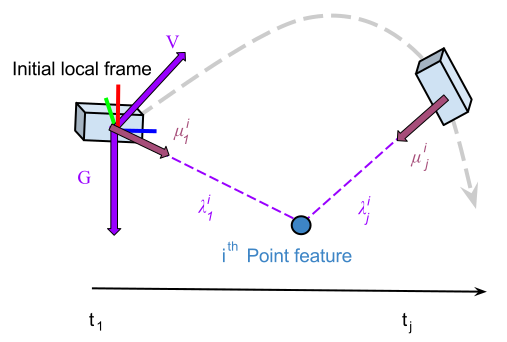
\includegraphics[width=0.7\columnwidth, trim={0 2cm 0 0}, clip]{images/closedFormExplained}
  \caption{Visual representation of Equation \ref{eq:final1}.
  The unknowns of the equation are colored in \textcolor{amethyst}{purple}.}
\end{figure}

Equation (\ref{eq:final1}) provides three scalar equations for each point feature $i=1,...,N$ and each frame starting from the second one $j=2,...n_i$.
We therefore have a linear system consisting of $3(n_i-1)N$ equations in $6 + Nn_i$ unknowns.
Indeed, note that, when the first frame is taken at $t_1 = 0$,
Equation (\ref{eq:final1}) is always satisfied; thus does not provide information.
We can write our system using matrix formulation.
Solving the system is equivalent to inverting a matrix of $3(n_i-1)N$ rows and $6+Nn_i$ columns.

In \cite{Martinelli2014}, the author proceeded to one more step before expressing the underlying linear system.
For a given frame $j$, the equation of the first point feature $i=1$ is subtracted from all other point feature equations $1<i \leq N$ (Equation (7)).
This additional step, very useful to detect system singularities, has the effect to corrupt all measurements with the first measurement,
hence worsening the performance of the closed-form solution. Therefore,
in this paper we discard this additional step.

The linear system in Equation (\ref{eq:final1}) can be written in the following compact form:

\begin{equation}
\label{eq:mat1}
\Xi X = S.
\end{equation}
\noindent Matrix $\Xi$ and vector $S$ are fully determined by the measurements, while $X$ is the unknown vector.
We have:

\begin{equation*}
  \begin{aligned}
S &\equiv [S_2^T, ...,S_2^T, S_3^T,...,S_3^T,...,S_{n_i}^T,...,S_{n_i}^T]^T \\
X &\equiv [ G^T, V^T, \lambda_1^1, ..., \lambda_1^N, ..., \lambda_{n_i}^1, ..., \lambda_{n_i}^N]^T
  \end{aligned}
\end{equation*}
\vspace{-1cm}

{
\arraycolsep=3pt % default: 5pt
\medmuskip = 1mu % default: 4mu plus 2mu minus 4mu
\begin{multline*}
  \Xi \equiv \\
      {
        \footnotesize
        \left[
          \begin{array}{l|l|l|l|l|l|l|l|l|l|l}
            T_2 & S_2 & \mu_1^1 & 0_3 & 0_3 & -\mu_2^1 & 0_3 & 0_3 & 0_3 & 0_3 & 0_3 \\
            T_2 & S_2 & 0_3 & \mu_1^2 & 0_3 & 0_3 & -\mu_2^2 & 0_3 & 0_3 & 0_3 & 0_3 \\
            ... & ... & ... & ... & ... & ... & ... & ... & ... & ... & ... \\
            T_2 & S_2 & 0_3 & 0_3 & \mu_1^N & 0_3 & 0_3 & -\mu_2^N & 0_3 & 0_3 & 0_3 \\
            ... & ... & ... & ... & ... & ... & ... & ... & ... & ... & ... \\
            ... & ... & ... & ... & ... & ... & ... & ... & ... & ... & ... \\
            T_{n_i} & S_{n_i} & \mu_1^1 & 0_3 & 0_3 & 0_3 & 0_3 & 0_3 & -\mu_{n_i}^1 & 0_3 & 0_3 \\
            T_{n_i} & S_{n_i} & 0_3 & \mu_1^2 & 0_3 & 0_3 & 0_3 & 0_3 & 0_3 & -\mu_{n_i}^2 & 0_3 \\
            ... & ... & ... & ... & ... & ... & ... & ... & ... & ... & ... \\
            T_{n_i} & S_{n_i} & 0_3 & 0_3 & \mu_1^N & 0_3 & 0_3 & 0_3 & 0_3 & 0_3 & -\mu_{n_i}^N
          \end{array}
          \right],
      }
\end{multline*}
}
\noindent where $T_j \equiv - \frac{t^2_j}{2} I_3$, $S_j \equiv -t_j I_3$ and $I_3$ is the identity $3\times 3$ matrix, $0_3$ is the $3\times 1$ zero matrix.
Note that matrix $\Xi$ and vector $S$ are slightly different from the ones proposed in \cite{Martinelli2014}.
This is due to the additional step that, as we explained in the previous paragraph, we discarded for numerical stability reasons (see \cite{Martinelli2014} section 3 for further details).

The sensor information is completely contained in the above linear system. Additionally, in \cite{Martinelli2014}, the author added a quadratic equation assuming the gravitational acceleration is a priori known.
Let us denote the gravitational magnitude by $g$.
We have the extra constraint $|G| = g$. We can express this constraint in matrix formulation:

\begin{equation}
\label{eq:mat2}
| \Pi X | ^2 = g^2,
\end{equation}

\noindent with $\Pi \equiv [I_3, 0_3, ..., 0_3]$. We can therefore recover the initial velocity, the roll and pitch angles, and the distances to the point features
by finding the vector $X$ that satisfies (\ref{eq:mat1}) and (\ref{eq:mat2}).

In the next sections, we will evaluate the performance of this method on simulated noisy sensor data.
This will allow us to identify its weaknesses and bring modifications to overcome them.

%% The system therefore becomes:

%% \begin{equation} \label{eq:final2}
%% \left[
%% \begin{array}{lcl}
%% S_j &=& \lambda_1^i\mu_1^i - V t_j - G \frac{t_j^2}{2} - \lambda^i_j \mu^i_j\\
%% 0_3 &=& \lambda_1^1\mu_1^1 - \lambda_j^1\mu_j^1 - \lambda_1^i\mu_1^i + \lambda^i_j \mu^i_j
%% \end{array}
%% \right.
%% \end{equation}



\section{LIMITATIONS OF \cite{Martinelli2014}}\label{SectionBottlenecks}

The goal of this section is to find out the limitations of the solution proposed in \cite{Martinelli2014} when it is adopted in a real scenario. In particular, special attention will be devoted to the case of an MAV equipped with low-cost camera and IMU sensors. For this reason, we perform simulations that significantly differ from the ones performed in \cite{Martinelli2014} (section $5.2$). Specifically, they differ because of the following two reasons:
\begin{itemize}
\item the simulated motion is the one of an MAV;
\item the values of the biases are significantly larger than the ones in \cite{Martinelli2014}.
\end{itemize}
This will allow us to evaluate the impact of the bias on the performance.

\subsection{Simulation setup}\label{SubsectionConsidered}

We simulate an MAV as a point particle executing a circular trajectory of about $1$m radius.

We measure our error on the absolute scale by computing the mean error over all estimated distances to point features $\lambda_j^i$.
We define the relative error as the euclidean distance between the estimation and the ground truth,
normalized by the ground truth.

Synthetic gyroscope and accelerometer data are affected by a statistical error of $0.5$ deg/s and $0.5$ cm/s\textsuperscript{2}, respectively and they are also corrupted by a constant bias.

We set $7$ simulated 3D point-features about $3$m away from the MAV, which flies at a speed of around $2~m~s^{-1}$.
We found that setting the frame rate of the simulated camera at 10Hz provides a sufficient pixel disparity with the following setup.
In practice, increasing the frame rate above 30Hz decreases the pixel disparity and introduces numerical instability for this setup.
The theoretical cases in which our system admits singularities are provided in \cite{Martinelli2012, Martinelli2014}.
Reducing the number of considered frames also reduces the size of the matrices and, thus, speeds up the computations.
As an example, over a time interval of 3 seconds, we obtain $31$ distinct frames.
When observing 7 features, solving the closed-form solution is equivalent to inverting a linear system of $3\times 30\times 7 = 630$ equations and $6+7\times 31=223$ unknowns (see section \ref{SectionCFS}).

The method we use to solve the overconstrained linear system $\Xi X = S$ is a Singular Value Decomposition (SVD) since it yields numerically robust solutions.

In the next section, we will present the results obtained with the original closed-form solution on the simulated data mentioned, with different sensor bias settings.
Our goal is to identify its performance limitations and introduce modifications to overcome them.


%% The case of a biased gyroscope is addressed in chapter \ref{ch:gyro}.
%% Indeed, the main contribution of this report is the simple method introduced in Section \ref{sec:computeBias} to compute the gyroscope bias with the closed-form solution, which happened to be a major performance bottleneck.

\subsection{Performance without bias}

The original closed-form solution described in Equation (\ref{eq:mat1}) will be used as a basis for our work.
Moreover, we can also use the knowledge of the gravity magnitude to refine our results (Equation (\ref{eq:mat2})).
In this case, we are minimizing a linear objective function with a quadratic constraint.
In Fig. \ref{fig:original}, we display the performance of the original Closed-Form (CF) solution in estimating speed, gravity in the local frame, and distances to the features with and without this additional constraint.

\begin{figure}
  \centering
    \resizebox{0.7\columnwidth}{!}{% This file was created by matlab2tikz.
% Minimal pgfplots version: 1.3
%
%The latest updates can be retrieved from
%  http://www.mathworks.com/matlabcentral/fileexchange/22022-matlab2tikz
%where you can also make suggestions and rate matlab2tikz.
%
%
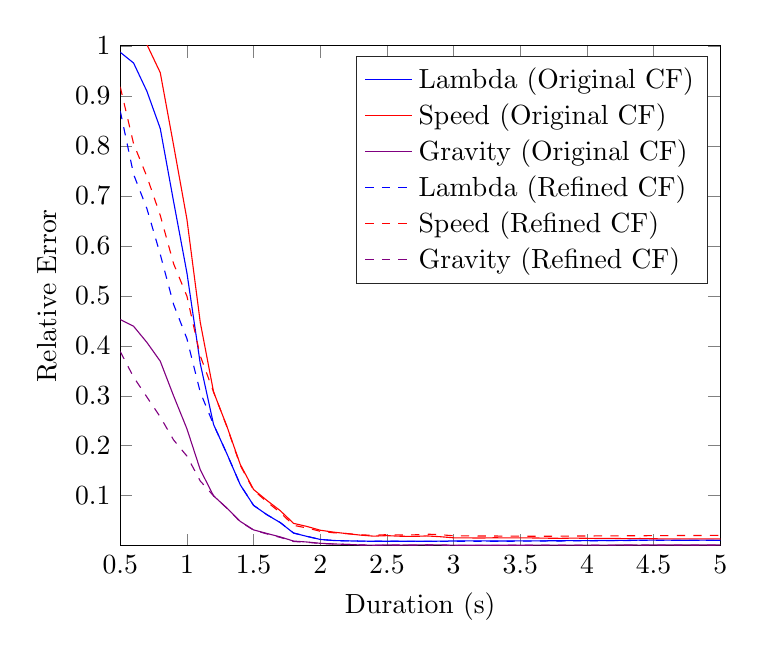
\begin{tikzpicture}

\begin{axis}[%
width= 3in,
height=2.5in,
at={(1.730625in,1.108021in)},
scale only axis,
xmin=0.5,
xmax=5,
xlabel={Duration (s)},
ymin=0,
ymax=1,
ylabel={Relative Error},
xtick={0.5,1,...,4.5,5},
ytick={0.1,0.2,...,1,1.1},
legend style={legend cell align=left,align=left,draw=white!15!black}
]
\addlegendimage{line legend,blue} % or mark=none?
\addlegendentry{Lambda (Original CF)}
\addlegendimage{line legend,red}
\addlegendentry{Speed (Original CF)}
\addlegendimage{line legend,color=violet}
\addlegendentry{Gravity (Original CF)}
\addlegendimage{line legend,blue, dashed} % or mark=none?
\addlegendentry{Lambda (Refined CF)}
\addlegendimage{line legend,red, dashed}
\addlegendentry{Speed (Refined CF)}
\addlegendimage{line legend,color=violet, dashed}
\addlegendentry{Gravity (Refined CF)}
\addplot [color=blue,solid]
  table[row sep=crcr]{%
0.5	0.986986753514567\\
0.6	0.965496175887839\\
0.7	0.908884988713299\\
0.8	0.834605900098789\\
0.9	0.688509687697423\\
1	0.545814308625612\\
1.1	0.364427179246033\\
1.2	0.242434411210129\\
1.3	0.183878592397401\\
1.4	0.121911048569874\\
1.5	0.0807353138595641\\
1.6	0.0620701781858337\\
1.7	0.0463123810228675\\
1.8	0.0253720031995344\\
1.9	0.0187770704730709\\
2	0.0126497125455335\\
2.1	0.010560679531817\\
2.2	0.00976540755882531\\
2.3	0.0093682520644791\\
2.4	0.00896475898455663\\
2.5	0.00904295045353062\\
2.6	0.0091019615864413\\
2.7	0.00917093321417799\\
2.8	0.00907743847898488\\
2.9	0.00918103828647361\\
3	0.00962574076068463\\
3.1	0.00966213914049497\\
3.2	0.00971702348607755\\
3.3	0.00958157226664205\\
3.4	0.00957300148692032\\
3.5	0.00975948413382532\\
3.6	0.0098284864131547\\
3.7	0.00994027840767147\\
3.8	0.0100230266098787\\
3.9	0.010335710280743\\
4	0.0103466285983591\\
4.1	0.0105213579285764\\
4.2	0.0105191124764209\\
4.3	0.0108984714686328\\
4.4	0.0112349258409643\\
4.5	0.0113237707239322\\
4.6	0.0111813738888987\\
4.7	0.0111055651935271\\
4.8	0.0111522184123338\\
4.9	0.0111634045711973\\
5	0.0110156371361694\\
};

\addplot [color=red,solid]
  table[row sep=crcr]{%
0.5	1.03985490942799\\
0.6	1.041598565655\\
0.7	1.00236650429721\\
0.8	0.946285206056902\\
0.9	0.801144005638605\\
1	0.653111424622228\\
1.1	0.446952652972\\
1.2	0.307545014749713\\
1.3	0.238764359391316\\
1.4	0.162775041374018\\
1.5	0.112552620250376\\
1.6	0.0906560408733978\\
1.7	0.0702325874714304\\
1.8	0.0448237845321961\\
1.9	0.0386534542271255\\
2	0.0311057395082368\\
2.1	0.027271305531551\\
2.2	0.0242870145505906\\
2.3	0.0213446569284375\\
2.4	0.019253423110833\\
2.5	0.0202639766987494\\
2.6	0.0190928884123492\\
2.7	0.0186673514534201\\
2.8	0.0196889505362513\\
2.9	0.0181422306527873\\
3	0.0159381584340546\\
3.1	0.0157920847297511\\
3.2	0.0154584974482486\\
3.3	0.015976038710748\\
3.4	0.0158808936479735\\
3.5	0.0157693091644158\\
3.6	0.0156439004935535\\
3.7	0.0151820539225519\\
3.8	0.0148957930996785\\
3.9	0.0153153750167038\\
4	0.014933953322141\\
4.1	0.0146764838709416\\
4.2	0.0147039369508963\\
4.3	0.0142241103735529\\
4.4	0.0144684009758614\\
4.5	0.0140030229426442\\
4.6	0.0138009121378266\\
4.7	0.0137979864770686\\
4.8	0.0138945374601937\\
4.9	0.0138179103318856\\
5	0.0136531794141864\\
};

\addplot [color=violet,solid]
  table[row sep=crcr]{%
0.5	0.45256728845443\\
0.6	0.438989841419345\\
0.7	0.406656156221457\\
0.8	0.369178138748777\\
0.9	0.29986163118787\\
1	0.23397552588102\\
1.1	0.152152611985808\\
1.2	0.0998104758119727\\
1.3	0.075363831899914\\
1.4	0.0487465324170283\\
1.5	0.0317722168426577\\
1.6	0.0246067693064432\\
1.7	0.0177358958515446\\
1.8	0.00939903099910719\\
1.9	0.00754012792012497\\
2	0.00496295120822077\\
2.1	0.00367655313659681\\
2.2	0.00272181300468793\\
2.3	0.00164880686826403\\
2.4	0.00110308489525322\\
2.5	0.00162151900958609\\
2.6	0.00143030127182418\\
2.7	0.00150270449784835\\
2.8	0.00195343381878727\\
2.9	0.00171570468150423\\
3	0.00116151685165242\\
3.1	0.00110349032753483\\
3.2	0.00113805096464642\\
3.3	0.00104326945703276\\
3.4	0.00104207400190048\\
3.5	0.00111948921944776\\
3.6	0.00117292771345839\\
3.7	0.00132349051181244\\
3.8	0.0013601718744057\\
3.9	0.00125277801498873\\
4	0.00131996805173955\\
4.1	0.00142381367611502\\
4.2	0.00143972237944171\\
4.3	0.00146394507122723\\
4.4	0.00143762761039746\\
4.5	0.00148630746570744\\
4.6	0.00151569200833691\\
4.7	0.00153601001684087\\
4.8	0.00153636716831822\\
4.9	0.00154925755573667\\
5	0.00156464565619423\\
};

\addplot [color=blue,dashed]
  table[row sep=crcr]{%
0.5	0.869558160556846\\
0.6	0.742870076857983\\
0.7	0.674183440707692\\
0.8	0.582912652968489\\
0.9	0.482789946367643\\
1	0.414182531262669\\
1.1	0.307145389889693\\
1.2	0.242445226349869\\
1.3	0.183885739484318\\
1.4	0.122001242924337\\
1.5	0.0808139804130309\\
1.6	0.0622084372713325\\
1.7	0.046458264083396\\
1.8	0.0255392106774605\\
1.9	0.0188945651124971\\
2	0.0126819776672027\\
2.1	0.0105582264010532\\
2.2	0.00977458541436067\\
2.3	0.00937162898341286\\
2.4	0.00893317495747788\\
2.5	0.00904602328223003\\
2.6	0.0089792615478916\\
2.7	0.00885631130482292\\
2.8	0.00890915689718858\\
2.9	0.00866700672171234\\
3	0.00898468634390109\\
3.1	0.00904265570992278\\
3.2	0.00907861279597341\\
3.3	0.00903566312187858\\
3.4	0.00904991007948833\\
3.5	0.00927462333580727\\
3.6	0.0093599983095238\\
3.7	0.00967464820082941\\
3.8	0.00961972571269459\\
3.9	0.00987299643701147\\
4	0.00987525810547274\\
4.1	0.0101668648074663\\
4.2	0.0102732311941265\\
4.3	0.010434550719291\\
4.4	0.0108283185325186\\
4.5	0.0109040767628152\\
4.6	0.0107776569270255\\
4.7	0.0107376717474263\\
4.8	0.0108177067637753\\
4.9	0.0107913870764718\\
5	0.0106083777057321\\
};
\addplot [color=red,dashed]
  table[row sep=crcr]{%
0.5	0.917809966701291\\
0.6	0.804024608842086\\
0.7	0.738280271673752\\
0.8	0.660809760146127\\
0.9	0.564146652502082\\
1	0.499236589213694\\
1.1	0.379960542953459\\
1.2	0.307533819150326\\
1.3	0.238070344260041\\
1.4	0.160881653106573\\
1.5	0.111129553747116\\
1.6	0.0877954468627039\\
1.7	0.0665295291853308\\
1.8	0.0409066831363829\\
1.9	0.0356222808569845\\
2	0.0289353511806837\\
2.1	0.025986230845492\\
2.2	0.0244057082778806\\
2.3	0.0219408049427895\\
2.4	0.0208600309177678\\
2.5	0.022258439253374\\
2.6	0.0216283224728915\\
2.7	0.0217711176749635\\
2.8	0.023233515944403\\
2.9	0.0222044737122673\\
3	0.0199415505442583\\
3.1	0.0198158447503515\\
3.2	0.0195215865774551\\
3.3	0.019481466324314\\
3.4	0.0193612567044837\\
3.5	0.0191425436198582\\
3.6	0.0191087403565778\\
3.7	0.019069067058095\\
3.8	0.0193198037130948\\
3.9	0.0194698786699845\\
4	0.0195999164865995\\
4.1	0.0197027401380329\\
4.2	0.0197452030020999\\
4.3	0.019969178829797\\
4.4	0.0200131394485748\\
4.5	0.0202971429206557\\
4.6	0.0204117363861295\\
4.7	0.0204607179083495\\
4.8	0.0205178656441319\\
4.9	0.0206288306616696\\
5	0.020756984562107\\
};
\addplot [color=violet,dashed]
  table[row sep=crcr]{%
0.5	0.38842359991127\\
0.6	0.337319237011632\\
0.7	0.297390660257021\\
0.8	0.257682276718495\\
0.9	0.211667138230797\\
1	0.179395868172561\\
1.1	0.129608223409189\\
1.2	0.0998229420683764\\
1.3	0.0750638135829617\\
1.4	0.0480063068352707\\
1.5	0.0313076781154105\\
1.6	0.0237456614340842\\
1.7	0.0167468628691132\\
1.8	0.00852855219340176\\
1.9	0.00698377853706011\\
2	0.00464365520024766\\
2.1	0.00352842730943088\\
2.2	0.00272964982301246\\
2.3	0.00166906391312137\\
2.4	0.00102145776312449\\
2.5	0.00153194748968682\\
2.6	0.001243769365914\\
2.7	0.00120849681016349\\
2.8	0.00160291053404673\\
2.9	0.00128269797201008\\
3	0.000747623899606023\\
3.1	0.000749819560237629\\
3.2	0.000915703070880042\\
3.3	0.000927235794556394\\
3.4	0.000947263644927916\\
3.5	0.00108303907498585\\
3.6	0.00114824878473496\\
3.7	0.00130823386965137\\
3.8	0.0013277442075085\\
3.9	0.00121481016265515\\
4	0.00126539634964563\\
4.1	0.00138104570693503\\
4.2	0.00140107982069819\\
4.3	0.00138045334053057\\
4.4	0.00136251610639204\\
4.5	0.00136694533363449\\
4.6	0.00138240513939476\\
4.7	0.00141193533192226\\
4.8	0.00142236013933898\\
4.9	0.00143435786486843\\
5	0.00144231219292143\\
};
\end{axis}
\end{tikzpicture}
}
    \caption{Original closed-form solution estimations with and without using the knowledge of the gravity (\ref{eq:mat2}). We are observing 7 features  over a variable duration of integration.\label{fig:original}}
\end{figure}

Note how the evaluations get better as we increase the integration time.
Indeed, our equations come from an extended triangulation \cite{Martinelli2012}.
Therefore, it requires a significant difference in the measurements over time to robustly estimate the state.


Without sensor bias, the original closed-form robustly estimates all the properties (below $0.1\%$ error) after $2$ seconds of integration.

Note that a robust estimation of the gravity requires a shorter duration of integration than the speed and the distance to the features.
In general, we found that the gravity is well estimated with the original closed-form solution due to its strong weight in the equations (see section \ref{sec:biasAcc}).
Therefore, constraining its magnitude does not improve the performance much.
In the following sections, we remove this constraint.



\subsection{Impact of accelerometer bias on the performance \label{sec:biasAcc}}
In order to visualize the impact of the accelerometer bias on the performance,
we corrupt the accelerometer measurements by a bias (Fig. \ref{fig:biasAccCF}).
Despite a high accelerometer bias, the closed-form solution still provides robust results.
As seen in Fig. \ref{fig:biasAccCF}, neither the estimation of the gravity, the velocity or the lambdas is impacted by the accelerometer bias.
To explain this behavior we ran many simulations by also considering trajectories that are not plausible for an MAV and by also changing the magnitude of the gravity. We found the following conclusions. When the rotations are small, the effect of a bias is negligible even if its value is larger than the inertial acceleration. This is easily explained by remarking that, in the case of negligible rotations, a bias on the accelerometer acts as the gravity. Hence, its impact depends on the ratio between its magnitude and the magnitude of the gravity.
If the rotations are important, the effect of a bias on the accelerometer is negligible when its magnitude is smaller than both the gravity and the inertial acceleration. Note that, for an MAV that accomplishes a loop of radius $1m$ and speed $2~m~s^{-1}$, the inertial acceleration is $4~m~s^{-2}$.

In \cite{Martinelli2014}, the author provides an alternative formulation of the closed-form solution including the accelerometer bias as an observable unknown of the system.
However, the estimation of the accelerometer bias with that method is not robust since our system is only slightly affected by it\footnote{Additionally, in \cite{Martinelli2014} property 12, we prove that rotations must occur around at least two independent axes to determine the bias. In general, for a motion of a few seconds, an MAV accomplishes rotations around a single axis.}.

\begin{figure}
  \centering
        \hspace{0.2\columnwidth}%
        \begin{subfigure}[b]{0.3\columnwidth}
                \resizebox{\columnwidth}{!}{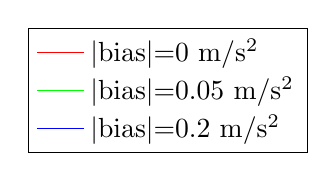
\begin{tikzpicture}
  \begin{customlegend}[legend entries={
        \textbar bias\textbar=0 m/s\textsuperscript{2},
        \textbar bias\textbar=0.05 m/s\textsuperscript{2},
        \textbar bias\textbar=0.2 m/s\textsuperscript{2}
      },
      legend cell align=left
    ]
    \addlegendimage{no markers,red}
    \addlegendimage{no markers,green}
    \addlegendimage{no markers,blue}
    \end{customlegend}
\end{tikzpicture}
}
                \caption{Legend}

        \end{subfigure}%
        \begin{subfigure}[b]{0.5\columnwidth}
                \resizebox{\columnwidth}{!}{% This file was created by matlab2tikz.
% Minimal pgfplots version: 1.3
%
%The latest updates can be retrieved from
%  http://www.mathworks.com/matlabcentral/fileexchange/22022-matlab2tikz
%where you can also make suggestions and rate matlab2tikz.
%
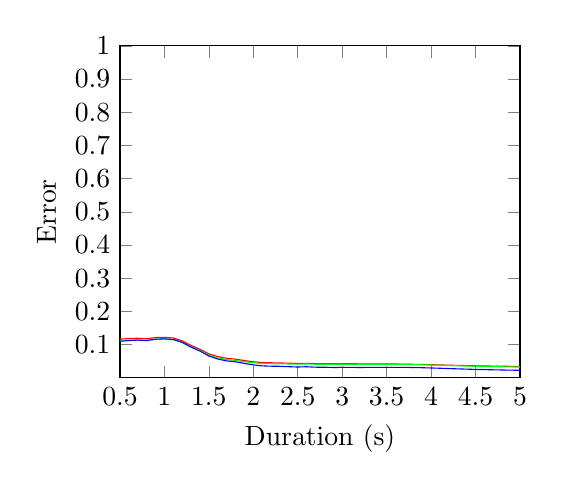
\begin{tikzpicture}

\begin{axis}[%
width= 2in,
height=1.66in,
at={(1.748842in,1.091895in)},
scale only axis,
xmin=0.5,
xmax=5,
xlabel={Duration (s)},
ytick={0.1,0.2,...,1,1.1},
xtick={0.5,1,...,4.5,5},
ymin=0,
ymax=1,
ylabel={Error},
title style={font=\bfseries},
legend style={legend cell align=left,align=left,draw=white!15!black}
]
\addplot [color=red,solid]
  table[row sep=crcr]{%
0.5	0.116606715060191\\
0.6	0.117997055105133\\
0.7	0.119102709903974\\
0.8	0.117525570741536\\
0.9	0.121125787159952\\
1	0.121848799026204\\
1.1	0.119844768728282\\
1.2	0.111293176404192\\
1.3	0.0972441692016664\\
1.4	0.0859201217596782\\
1.5	0.0719646971135904\\
1.6	0.0637925808506565\\
1.7	0.0587015571115359\\
1.8	0.056129189693083\\
1.9	0.0517798779009592\\
2	0.0482428904558047\\
2.1	0.0459797767399953\\
2.2	0.0451793517777765\\
2.3	0.0447058868379019\\
2.4	0.0438928826447229\\
2.5	0.0432485444401573\\
2.6	0.0435265998149818\\
2.7	0.0427019585418582\\
2.8	0.0426023542762414\\
2.9	0.0422630060176831\\
3	0.0422846181084555\\
3.1	0.0423041821959344\\
3.2	0.0420313721723238\\
3.3	0.0420868715251723\\
3.4	0.041845126835783\\
3.5	0.0417458915459075\\
3.6	0.0414308377400679\\
3.7	0.0411605921677774\\
3.8	0.0406069606036085\\
3.9	0.040013333767894\\
4	0.0393799772584942\\
4.1	0.0386907117981665\\
4.2	0.0379690145312799\\
4.3	0.0372910309735248\\
4.4	0.0366612662345494\\
4.5	0.036128938670861\\
4.6	0.035643285428503\\
4.7	0.0352075823255911\\
4.8	0.0347925486691523\\
4.9	0.0343939177741983\\
5	0.0341009792987977\\
};

%% \addlegendentry{\textbar bias\textbar=0};
\addplot [color=green,solid]
  table[row sep=crcr]{%
0.5	0.111629840333276\\
0.6	0.112941864217596\\
0.7	0.113999807359034\\
0.8	0.112401380716064\\
0.9	0.116039605389351\\
1	0.116821828487753\\
1.1	0.114901886148879\\
1.2	0.106446823821964\\
1.3	0.0925020301438534\\
1.4	0.081328558321378\\
1.5	0.0675516306037404\\
1.6	0.0595873966546359\\
1.7	0.0546893379224739\\
1.8	0.05233537519754\\
1.9	0.0482654296101405\\
2	0.0450379587938784\\
2.1	0.0430548359597281\\
2.2	0.0424590786680326\\
2.3	0.0421947777391173\\
2.4	0.0415724003923388\\
2.5	0.0411086546402141\\
2.6	0.0414965285365714\\
2.7	0.04085355568415\\
2.8	0.0408900976173342\\
2.9	0.0406790980406572\\
3	0.0408023651753037\\
3.1	0.040898540448454\\
3.2	0.0407386835119184\\
3.3	0.0408856900140973\\
3.4	0.0407055325787586\\
3.5	0.0406650688348556\\
3.6	0.0404025123480414\\
3.7	0.0401733262397001\\
3.8	0.0396314916571967\\
3.9	0.0390295938996\\
4	0.0383633615268031\\
4.1	0.0376379818458523\\
4.2	0.0368568157558358\\
4.3	0.0361050422745377\\
4.4	0.0354024030978923\\
4.5	0.0347817174123263\\
4.6	0.0342101140609905\\
4.7	0.033689405446034\\
4.8	0.0331949095418029\\
4.9	0.0327254959480877\\
5	0.0323533125743179\\
};
%% \addlegendentry{\textbar bias\textbar=0.05};

\addplot [color=blue,solid]
  table[row sep=crcr]{%
0.5	0.110205400460866\\
0.6	0.112059900874519\\
0.7	0.113445719597403\\
0.8	0.112196475852541\\
0.9	0.116185877950009\\
1	0.117178160150115\\
1.1	0.11540696886235\\
1.2	0.106864098599073\\
1.3	0.0923154592425234\\
1.4	0.0805508028389122\\
1.5	0.065674696763059\\
1.6	0.0565667683528162\\
1.7	0.0508590366634676\\
1.8	0.0481998958516259\\
1.9	0.0431166259404963\\
2	0.038744369905904\\
2.1	0.0358755619489716\\
2.2	0.0349167873159606\\
2.3	0.0345441744362363\\
2.4	0.0333996497756916\\
2.5	0.0324446398493226\\
2.6	0.0332340318487519\\
2.7	0.0319130081585281\\
2.8	0.0317762965859852\\
2.9	0.0310083577332042\\
3	0.0312478312313894\\
3.1	0.0313936412022642\\
3.2	0.030907768925086\\
3.3	0.0314917173744273\\
3.4	0.0311995738137807\\
3.5	0.031473719274027\\
3.6	0.031363804975408\\
3.7	0.0314509194095001\\
3.8	0.0309137299278705\\
3.9	0.0303162604615932\\
4	0.029549362213877\\
4.1	0.0287510007535127\\
4.2	0.027765935199653\\
4.3	0.0268347945146144\\
4.4	0.0260330332508285\\
4.5	0.0252621868822711\\
4.6	0.0246041161786416\\
4.7	0.0240225065899942\\
4.8	0.023483896835938\\
4.9	0.0229749792550578\\
5	0.0225526570431922\\
};
%% \addlegendentry{\textbar bias\textbar=0.2};

\end{axis}
\end{tikzpicture}%
}
                \caption{Gravity estimation error}

        \end{subfigure}
        ~
        \begin{subfigure}[b]{0.5\columnwidth}
                \resizebox{\columnwidth}{!}{% This file was created by matlab2tikz.
% Minimal pgfplots version: 1.3
%
%The latest updates can be retrieved from
%  http://www.mathworks.com/matlabcentral/fileexchange/22022-matlab2tikz
%where you can also make suggestions and rate matlab2tikz.
%
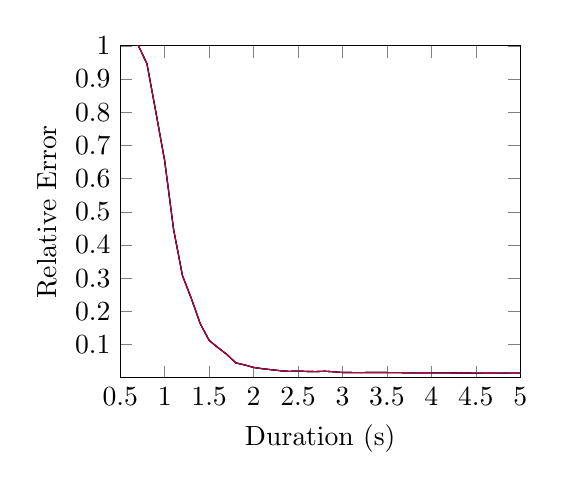
\begin{tikzpicture}

\begin{axis}[%
width= 2in,
height=1.66in,
at={(1.751579in,1.09421in)},
scale only axis,
xmin=0.5,
xmax=5,
xlabel={Duration (s)},
ytick={0.1,0.2,...,1,1.1},
xtick={0.5,1,...,4.5,5},
ymin=0,
ymax=1,
ylabel={Relative Error},
title style={font=\bfseries},
legend style={legend cell align=left,align=left,draw=white!15!black}
  ]
\addplot [color=red,solid]
  table[row sep=crcr]{%
0.5	1.03985490942799\\
0.6	1.041598565655\\
0.7	1.00236650429721\\
0.8	0.946285206056902\\
0.9	0.801144005638605\\
1	0.653111424622228\\
1.1	0.446952652972\\
1.2	0.307545014749713\\
1.3	0.238764359391316\\
1.4	0.162775041374018\\
1.5	0.112552620250376\\
1.6	0.0906560408733978\\
1.7	0.0702325874714304\\
1.8	0.0448237845321961\\
1.9	0.0386534542271255\\
2	0.0311057395082368\\
2.1	0.027271305531551\\
2.2	0.0242870145505906\\
2.3	0.0213446569284375\\
2.4	0.019253423110833\\
2.5	0.0202639766987494\\
2.6	0.0190928884123492\\
2.7	0.0186673514534201\\
2.8	0.0196889505362513\\
2.9	0.0181422306527873\\
3	0.0159381584340546\\
3.1	0.0157920847297511\\
3.2	0.0154584974482486\\
3.3	0.015976038710748\\
3.4	0.0158808936479735\\
3.5	0.0157693091644158\\
3.6	0.0156439004935535\\
3.7	0.0151820539225519\\
3.8	0.0148957930996785\\
3.9	0.0153153750167038\\
4	0.014933953322141\\
4.1	0.0146764838709416\\
4.2	0.0147039369508963\\
4.3	0.0142241103735529\\
4.4	0.0144684009758614\\
4.5	0.0140030229426442\\
4.6	0.0138009121378266\\
4.7	0.0137979864770686\\
4.8	0.0138945374601937\\
4.9	0.0138179103318856\\
5	0.0136531794141864\\
  };

\addplot [color=green,solid]
  table[row sep=crcr]{%
0.5	1.03985958098901\\
0.6	1.04160318355915\\
0.7	1.00237106009902\\
0.8	0.946289717389913\\
0.9	0.801148482808236\\
1	0.653115835094683\\
1.1	0.446956963215328\\
1.2	0.307549193614189\\
1.3	0.238768402671388\\
1.4	0.162778866000266\\
1.5	0.112556164989696\\
1.6	0.0906594511027657\\
1.7	0.0702357530206231\\
1.8	0.0448262850837141\\
1.9	0.0386556163799586\\
2	0.0311072877769502\\
2.1	0.0272723706785286\\
2.2	0.0242875971735912\\
2.3	0.0213446348227341\\
2.4	0.0192528393894945\\
2.5	0.0202634686746629\\
2.6	0.0190921269501307\\
2.7	0.0186664007188528\\
2.8	0.0196879239235448\\
2.9	0.0181410206611039\\
3	0.0159368124813167\\
3.1	0.0157906956206664\\
3.2	0.0154572915599915\\
3.3	0.015974943255289\\
3.4	0.0158797897599564\\
3.5	0.0157684278283326\\
3.6	0.0156430872283733\\
3.7	0.0151814885198358\\
3.8	0.014895146078053\\
3.9	0.0153144793914982\\
4	0.0149330818265368\\
4.1	0.0146758551046747\\
4.2	0.0147033461899024\\
4.3	0.0142233401735353\\
4.4	0.0144675984784877\\
4.5	0.0140021327931907\\
4.6	0.0138000012779865\\
4.7	0.0137971317684698\\
4.8	0.0138936794965301\\
4.9	0.0138170217044604\\
5	0.0136522219455462\\
  };

\addplot [color=blue,solid]
  table[row sep=crcr]{%
0.5	1.03986425207895\\
0.6	1.04160780091446\\
0.7	1.00237561027151\\
0.8	0.946294222676901\\
0.9	0.801152949003822\\
1	0.653120236997524\\
1.1	0.446961263559742\\
1.2	0.307553365956837\\
1.3	0.238772442420924\\
1.4	0.162782689585394\\
1.5	0.112559710919862\\
1.6	0.0906628620508701\\
1.7	0.0702389182838786\\
1.8	0.0448287832679672\\
1.9	0.0386577757661939\\
2	0.0311088319409189\\
2.1	0.0272734304054249\\
2.2	0.0242881740428105\\
2.3	0.0213446052217924\\
2.4	0.0192522476329966\\
2.5	0.0202629559685031\\
2.6	0.0190913614801648\\
2.7	0.0186654480077921\\
2.8	0.0196868997231422\\
2.9	0.0181398119199815\\
3	0.0159354608914177\\
3.1	0.0157892997710918\\
3.2	0.015456077806116\\
3.3	0.01597383905107\\
3.4	0.0158786758680475\\
3.5	0.0157675355582793\\
3.6	0.0156422624238909\\
3.7	0.0151809113268135\\
3.8	0.0148944876096839\\
3.9	0.0153135721746979\\
4	0.0149321986923262\\
4.1	0.0146752151128445\\
4.2	0.0147027437569585\\
4.3	0.0142225582675433\\
4.4	0.0144667839076757\\
4.5	0.014001231209046\\
4.6	0.0137990789502391\\
4.7	0.0137962654346151\\
4.8	0.0138928097441045\\
4.9	0.0138161214008475\\
5	0.0136512527044398\\
  };

\addplot [color=black,solid]
  table[row sep=crcr]{%
0.5	1.03990162657298\\
0.6	1.04164474499346\\
0.7	1.00241202605313\\
0.8	0.946330255505779\\
0.9	0.801188651450575\\
1	0.653155418577664\\
1.1	0.44699564265194\\
1.2	0.307586738342365\\
1.3	0.238804769430305\\
1.4	0.162813294486986\\
1.5	0.112588099592512\\
1.6	0.0906901780032391\\
1.7	0.0702642726824345\\
1.8	0.0448488150337778\\
1.9	0.0386750988110832\\
2	0.0311212462405861\\
2.1	0.0272819801300415\\
2.2	0.0242928691246088\\
2.3	0.0213444647144645\\
2.4	0.0192476184012775\\
2.5	0.0202589351236235\\
2.6	0.0190853167280258\\
2.7	0.0186578952976754\\
2.8	0.019678747951536\\
2.9	0.0181301988233346\\
3	0.0159247584460048\\
3.1	0.0157782557374192\\
3.2	0.0154465046811283\\
3.3	0.0159651499258818\\
3.4	0.0158699220172952\\
3.5	0.0157605641007467\\
3.6	0.0156358378887817\\
3.7	0.0151764725213243\\
3.8	0.0148894013626436\\
3.9	0.0153064978034355\\
4	0.0149253210350167\\
4.1	0.0146702818693963\\
4.2	0.0146981137461654\\
4.3	0.0142164986112002\\
4.4	0.0144604637985282\\
4.5	0.0139942166176036\\
4.6	0.0137919001856516\\
4.7	0.0137895344889111\\
4.8	0.0138860507471762\\
4.9	0.0138091176101833\\
5	0.0136436989435932\\
  };

\addplot [color=purple,solid]
  table[row sep=crcr]{%
0.5	1.0399483433515\\
0.6	1.04169092245013\\
0.7	1.00245754542336\\
0.8	0.946375306304471\\
0.9	0.801233300755678\\
1	0.65319942001106\\
1.1	0.447038642504946\\
1.2	0.307628474533131\\
1.3	0.238845193954841\\
1.4	0.162851572957107\\
1.5	0.112623619899911\\
1.6	0.0907243680947724\\
1.7	0.0702960220793722\\
1.8	0.0448739356682219\\
1.9	0.0386968432854359\\
2	0.031136873332547\\
2.1	0.0272927883706028\\
2.2	0.0242988703409776\\
2.3	0.021344435140119\\
2.4	0.0192419882631464\\
2.5	0.0202540553915376\\
2.6	0.019077913510439\\
2.7	0.018648608793286\\
2.8	0.01966870426995\\
2.9	0.0181183393990501\\
3	0.015911557573295\\
3.1	0.015764629585974\\
3.2	0.0154347246807435\\
3.3	0.0159544706566606\\
3.4	0.0158591630136393\\
3.5	0.0157520374104561\\
3.6	0.0156279970977605\\
3.7	0.0151711224971348\\
3.8	0.0148832452227136\\
3.9	0.0152978479177686\\
4	0.0149169231583479\\
4.1	0.0146643221623784\\
4.2	0.0146925342577677\\
4.3	0.014209138691543\\
4.4	0.014452775411792\\
4.5	0.0139856678843345\\
4.6	0.01378315079938\\
4.7	0.0137813471009242\\
4.8	0.013877827820372\\
4.9	0.0138005907812756\\
5	0.0136344876929685\\
  };

\end{axis}
\end{tikzpicture}%
}
                \caption{Velocity estimation error}

        \end{subfigure}%
        \begin{subfigure}[b]{0.5\columnwidth}
                \resizebox{\columnwidth}{!}{% This file was created by matlab2tikz.
% Minimal pgfplots version: 1.3
%
%The latest updates can be retrieved from
%  http://www.mathworks.com/matlabcentral/fileexchange/22022-matlab2tikz
%where you can also make suggestions and rate matlab2tikz.
%
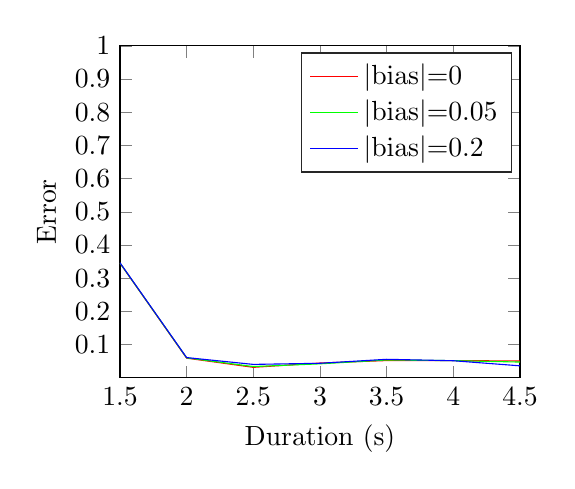
\begin{tikzpicture}

\begin{axis}[%
width= 2in,
height=1.66in,
at={(1.751579in,1.09421in)},
scale only axis,
xmin=1.5,
xmax=4.5,
xlabel={Duration (s)},
ytick={0.1,0.2,...,1,1.1},
xtick={1.5,2,...,4,4.5},
ymin=0,
ymax=1,
ylabel={Error},
title style={font=\bfseries},
legend style={legend cell align=left,align=left,draw=white!15!black}
]
\addplot [color=red,solid]
  table[row sep=crcr]{%
1.5	0.345420505285925\\
2	0.0591269666437189\\
2.5	0.0314634761572925\\
3	0.0443930698554671\\
3.5	0.0518808728966365\\
4	0.0517486442145949\\
4.5	0.0506422188840558\\
};
\addlegendentry{\textbar bias\textbar=0};

\addplot [color=green,solid]
  table[row sep=crcr]{%
1.5	0.345695555937959\\
2	0.060086124212135\\
2.5	0.0337940864201277\\
3	0.0419967425836958\\
3.5	0.0537493965525162\\
4	0.0516342878613844\\
4.5	0.0473833798683534\\
};
\addlegendentry{\textbar bias\textbar=0.05};

\addplot [color=blue,solid]
  table[row sep=crcr]{%
1.5	0.346564570148642\\
2	0.0608748726887488\\
2.5	0.0403201005186154\\
3	0.0436805564269853\\
3.5	0.0556848387804751\\
4	0.0513853623130932\\
4.5	0.0360060396972207\\
};
\addlegendentry{\textbar bias\textbar=0.2};

\end{axis}
\end{tikzpicture}%
}
                \caption{Lambda estimation error}

        \end{subfigure}
        \caption{Impact of the accelerometer bias on the performance of the closed-form solution. We are observing 7 features  over a variable duration of integration.\label{fig:biasAccCF}}
\end{figure}



\subsection{Impact of gyroscope bias on the performance}
To visualize the impact of the gyroscope bias on the performance,
we corrupt the gyroscope measurements by an artificial bias (Fig. \ref{fig:biasGyroCF}).

%Our experiments have shown that the presence of gyroscope bias significantly damages the results of the closed-form solution.

\begin{figure}
  \centering
        \hspace{0.2\columnwidth}%
        \begin{subfigure}[b]{0.3\columnwidth}
                \resizebox{\columnwidth}{!}{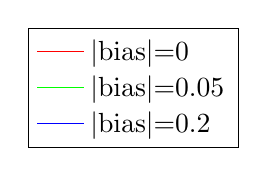
\begin{tikzpicture}
  \begin{customlegend}[legend entries={
        \textbar bias\textbar=0,
        \textbar bias\textbar=0.05,
        \textbar bias\textbar=0.2
      },
      legend cell align=left
    ]
    \addlegendimage{no markers,red}
    \addlegendimage{no markers,green}
    \addlegendimage{no markers,blue}
    \end{customlegend}
\end{tikzpicture}
}
                \caption{Legend}

        \end{subfigure}%
        \begin{subfigure}[b]{0.5\columnwidth}
                \resizebox{\columnwidth}{!}{% This file was created by matlab2tikz.
% Minimal pgfplots version: 1.3
%
%The latest updates can be retrieved from
%  http://www.mathworks.com/matlabcentral/fileexchange/22022-matlab2tikz
%where you can also make suggestions and rate matlab2tikz.
%
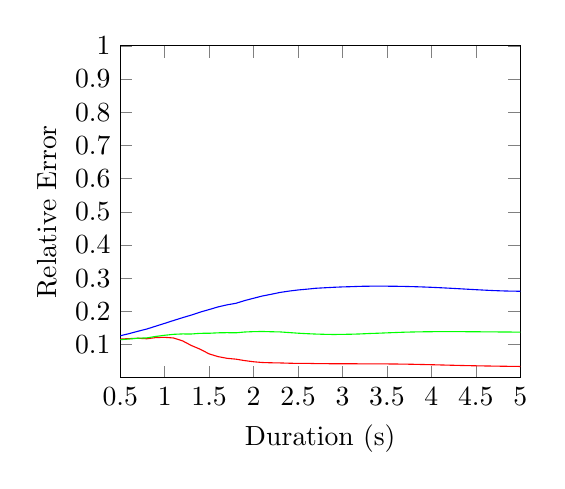
\begin{tikzpicture}

\begin{axis}[%
width= 2in,
height=1.66in,
at={(0.873053in,1.091895in)},
scale only axis,
xmin=0.5,
xmax=5,
xlabel={Duration (s)},
ytick={0.1,0.2,...,1,1.1},
xtick={0.5,1,...,4.5,5},
ymin=0,
ymax=1,
ylabel={Relative Error},
title style={font=\bfseries},
legend style={legend cell align=left,align=left,draw=white!15!black}
]
\addplot [color=red,solid]
  table[row sep=crcr]{%
0.5	0.116606715060191\\
0.6	0.117997055105133\\
0.7	0.119102709903974\\
0.8	0.117525570741536\\
0.9	0.121125787159952\\
1	0.121848799026204\\
1.1	0.119844768728282\\
1.2	0.111293176404192\\
1.3	0.0972441692016664\\
1.4	0.0859201217596782\\
1.5	0.0719646971135904\\
1.6	0.0637925808506565\\
1.7	0.0587015571115359\\
1.8	0.056129189693083\\
1.9	0.0517798779009592\\
2	0.0482428904558047\\
2.1	0.0459797767399953\\
2.2	0.0451793517777765\\
2.3	0.0447058868379019\\
2.4	0.0438928826447229\\
2.5	0.0432485444401573\\
2.6	0.0435265998149818\\
2.7	0.0427019585418582\\
2.8	0.0426023542762414\\
2.9	0.0422630060176831\\
3	0.0422846181084555\\
3.1	0.0423041821959344\\
3.2	0.0420313721723238\\
3.3	0.0420868715251723\\
3.4	0.041845126835783\\
3.5	0.0417458915459075\\
3.6	0.0414308377400679\\
3.7	0.0411605921677774\\
3.8	0.0406069606036085\\
3.9	0.040013333767894\\
4	0.0393799772584942\\
4.1	0.0386907117981665\\
4.2	0.0379690145312799\\
4.3	0.0372910309735248\\
4.4	0.0366612662345494\\
4.5	0.036128938670861\\
4.6	0.035643285428503\\
4.7	0.0352075823255911\\
4.8	0.0347925486691523\\
4.9	0.0343939177741983\\
5	0.0341009792987977\\
};

%% \addlegendentry{\textbar bias\textbar =0};

\addplot [color=green,solid]
  table[row sep=crcr]{%
0.5	0.114794687547566\\
0.6	0.116779562670337\\
0.7	0.119185926413267\\
0.8	0.120120531727668\\
0.9	0.124610537501479\\
1	0.128052587957767\\
1.1	0.130926249443556\\
1.2	0.132078989798618\\
1.3	0.13192738084419\\
1.4	0.133950631948478\\
1.5	0.13407339510689\\
1.6	0.135451152760844\\
1.7	0.135876030068171\\
1.8	0.135476169238146\\
1.9	0.137907159471493\\
2	0.139008951294816\\
2.1	0.139465057704968\\
2.2	0.138679837236883\\
2.3	0.138093777901368\\
2.4	0.136212293045122\\
2.5	0.134306983207276\\
2.6	0.132848519704814\\
2.7	0.131699711866214\\
2.8	0.130920639935682\\
2.9	0.130421144778009\\
3	0.13078357013329\\
3.1	0.131253433397877\\
3.2	0.132089254038683\\
3.3	0.133355246577893\\
3.4	0.134215771247405\\
3.5	0.135345848264681\\
3.6	0.136359990672705\\
3.7	0.13735842784796\\
3.8	0.138002328772655\\
3.9	0.138489998145827\\
4	0.138794692629325\\
4.1	0.139006466534816\\
4.2	0.139021487405358\\
4.3	0.138926226194958\\
4.4	0.138800619376313\\
4.5	0.138616410667534\\
4.6	0.138405101734246\\
4.7	0.138178913135068\\
4.8	0.137949251009142\\
4.9	0.137750866645688\\
5	0.137634226533832\\
};
%% \addlegendentry{\textbar bias\textbar =0.05};

\addplot [color=blue,solid]
  table[row sep=crcr]{%
0.5	0.126540731489485\\
0.6	0.133059738131836\\
0.7	0.140191754416727\\
0.8	0.146993315210864\\
0.9	0.155514639755021\\
1	0.163943481621357\\
1.1	0.172603931314876\\
1.2	0.180994199517491\\
1.3	0.188952369328098\\
1.4	0.197870605066536\\
1.5	0.205499151242719\\
1.6	0.213456391224108\\
1.7	0.219618286221541\\
1.8	0.224293131663155\\
1.9	0.232533006914849\\
2	0.239594926602202\\
2.1	0.246385580596315\\
2.2	0.251619874636628\\
2.3	0.257204117125385\\
2.4	0.26116409581935\\
2.5	0.264500898715111\\
2.6	0.266903237389395\\
2.7	0.26963606191249\\
2.8	0.271118335838816\\
2.9	0.272560083765427\\
3	0.27373393339939\\
3.1	0.27445990331874\\
3.2	0.275477563174396\\
3.3	0.275863566646588\\
3.4	0.276042083151684\\
3.5	0.275903152314242\\
3.6	0.27565649154562\\
3.7	0.275145916729527\\
3.8	0.274474577722157\\
3.9	0.273601323214602\\
4	0.272523860177769\\
4.1	0.271275440688065\\
4.2	0.269875684720536\\
4.3	0.268394660815776\\
4.4	0.26687737570394\\
4.5	0.265365118898912\\
4.6	0.263948120121799\\
4.7	0.262694142312051\\
4.8	0.261675381813738\\
4.9	0.260977458906844\\
5	0.260686548115178\\
};
%% \addlegendentry{\textbar bias\textbar =0.2};


\end{axis}
\end{tikzpicture}%
}
                \caption{Gravity estimation error}

        \end{subfigure}
        ~
        \begin{subfigure}[b]{0.5\columnwidth}
                \resizebox{\columnwidth}{!}{% This file was created by matlab2tikz.
% Minimal pgfplots version: 1.3
%
%The latest updates can be retrieved from
%  http://www.mathworks.com/matlabcentral/fileexchange/22022-matlab2tikz
%where you can also make suggestions and rate matlab2tikz.
%
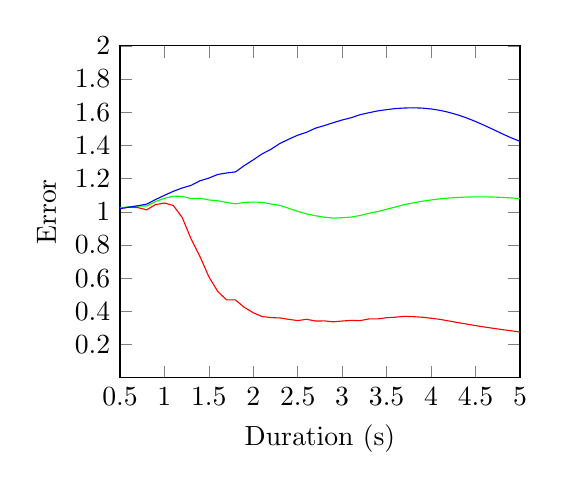
\begin{tikzpicture}

\begin{axis}[%
width= 2in,
height=1.66in,
at={(1.751579in,1.09421in)},
scale only axis,
unbounded coords=jump,
xmin=0.5,
xmax=5,
xlabel={Duration (s)},
ytick={0.2,0.4,...,1.8,2},
xtick={0.5,1,...,4.5,5},
ymin=0,
ymax=2,
ylabel={Error },
title style={font=\bfseries},
legend style={legend cell align=left,align=left,draw=white!15!black, at={(0.02,0.98)},anchor=north west}
]
\addplot [color=red,solid]
  table[row sep=crcr]{%
0.5	1.02175935565935\\
0.6	1.02791398584138\\
0.7	1.0256631041239\\
0.8	1.0119346333155\\
0.9	1.04321328865705\\
1	1.05305292291286\\
1.1	1.03815288783518\\
1.2	0.966235430882726\\
1.3	0.837047486448539\\
1.4	0.731229109725668\\
1.5	0.609284597782465\\
1.6	0.520318182824509\\
1.7	0.469135917702167\\
1.8	0.469085329131466\\
1.9	0.42429147636652\\
2	0.391855665299047\\
2.1	0.36905483808771\\
2.2	0.362779296792721\\
2.3	0.360542053306133\\
2.4	0.352030822201322\\
2.5	0.34487514314054\\
2.6	0.352486455310822\\
2.7	0.341992321163803\\
2.8	0.342831852614327\\
2.9	0.337300894873511\\
3	0.342135595088423\\
3.1	0.346018229140361\\
3.2	0.344320001070864\\
3.3	0.35468093595922\\
3.4	0.35488052155194\\
3.5	0.362036618911888\\
3.6	0.365160051746595\\
3.7	0.370578427179208\\
3.8	0.368363808036823\\
3.9	0.364986989708309\\
4	0.358867362407108\\
4.1	0.35230509491568\\
4.2	0.342589674214479\\
4.3	0.332678414221663\\
4.4	0.324003459162384\\
4.5	0.31454121832915\\
4.6	0.306091641043392\\
4.7	0.298130318170641\\
4.8	0.290540234885821\\
4.9	0.283328674546198\\
5	0.276133555094666\\
};
%% \addlegendentry{\textbar bias\textbar =0};

\addplot [color=green,solid]
  table[row sep=crcr]{%
0.5	1.02355207120059\\
0.6	1.03026860460552\\
0.7	1.03498841697354\\
0.8	1.03509865794458\\
0.9	1.06188179612969\\
1	1.08137067759546\\
1.1	1.09434528062304\\
1.2	1.09308614745031\\
1.3	1.07957133707453\\
1.4	1.08198629413277\\
1.5	1.07139175284461\\
1.6	1.06668737595967\\
1.7	1.0563822441038\\
1.8	1.04773112707274\\
1.9	1.05666989948084\\
2	1.05891389555878\\
2.1	1.05704076871567\\
2.2	1.04677684684384\\
2.3	1.0385257163595\\
2.4	1.02101065429131\\
2.5	1.00320585632867\\
2.6	0.987609688193366\\
2.7	0.976083363282641\\
2.8	0.967448011136072\\
2.9	0.961970778979797\\
3	0.964296165161102\\
3.1	0.968356703561008\\
3.2	0.977512329694832\\
3.3	0.991113113208863\\
3.4	1.00176372953356\\
3.5	1.0156246142103\\
3.6	1.02929430368843\\
3.7	1.04323363677726\\
3.8	1.05415319757685\\
3.9	1.06366706258245\\
4	1.07138552207739\\
4.1	1.07840513670921\\
4.2	1.08322640543848\\
4.3	1.0864422067885\\
4.4	1.08893879589077\\
4.5	1.0900916141486\\
4.6	1.0901160099761\\
4.7	1.08897843891426\\
4.8	1.08669231465207\\
4.9	1.08357561529757\\
5	1.07995032930589\\
};
%% \addlegendentry{\textbar bias\textbar =0.05};

\addplot [color=blue,solid]
  table[row sep=crcr]{%
0.5	1.01877763456232\\
0.6	1.0278748430534\\
0.7	1.03647684104063\\
0.8	1.04607509094039\\
0.9	1.07373182381123\\
1	1.0992378890232\\
1.1	1.12343639507097\\
1.2	1.14342836985361\\
1.3	1.15939843048576\\
1.4	1.18666195550943\\
1.5	1.20323355742176\\
1.6	1.22500916552771\\
1.7	1.23403164608103\\
1.8	1.24038676187243\\
1.9	1.27889382750531\\
2	1.31306054720695\\
2.1	1.34914949398501\\
2.2	1.37695229929848\\
2.3	1.41185295747137\\
2.4	1.43756656712845\\
2.5	1.46153871693893\\
2.6	1.47940128627451\\
2.7	1.50401782236624\\
2.8	1.5194677618903\\
2.9	1.5370086354038\\
3	1.55311037909986\\
3.1	1.56657245737693\\
3.2	1.58481513240264\\
3.3	1.59680156574203\\
3.4	1.6079711404209\\
3.5	1.61549676163322\\
3.6	1.62211616486494\\
3.7	1.62523473960433\\
3.8	1.62657662735924\\
3.9	1.62480370752791\\
4	1.61971926464314\\
4.1	1.61118324728822\\
4.2	1.59924533292031\\
4.3	1.584037537904\\
4.4	1.56559303673026\\
4.5	1.54422341843541\\
4.6	1.52064171983436\\
4.7	1.49566043709397\\
4.8	1.47029525716865\\
4.9	1.44602524985353\\
5	1.4247661626196\\
};
%% \addlegendentry{\textbar bias\textbar=0.2};

%% \node at (axis cs:3.2,0.3) {\color{blue}\textbar bias\textbar=0.2 off chart};

\end{axis}
\end{tikzpicture}%
}
                \caption{Velocity estimation error}

        \end{subfigure}%
        \begin{subfigure}[b]{0.5\columnwidth}
                \resizebox{\columnwidth}{!}{% This file was created by matlab2tikz.
% Minimal pgfplots version: 1.3
%
%The latest updates can be retrieved from
%  http://www.mathworks.com/matlabcentral/fileexchange/22022-matlab2tikz
%where you can also make suggestions and rate matlab2tikz.
%
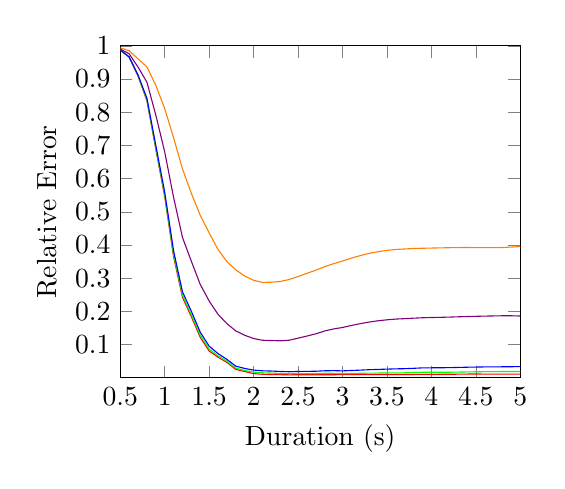
\begin{tikzpicture}

\begin{axis}[%
width= 2in,
height=1.66in,
at={(0.873053in,1.091895in)},
scale only axis,
xmin=0.5,
xmax=5,
xlabel={Duration (s)},
ytick={0.1,0.2,...,1,1.1},
xtick={0.5,1,...,4.5,5},
ymin=0,
ymax=1,
ylabel={Relative Error},
title style={font=\bfseries},
legend style={legend cell align=left,align=left,draw=white!15!black, at={(0.02,0.02)},anchor=south west}
]
\addplot [color=red,solid]
  table[row sep=crcr]{%
0.5	0.986986753514567\\
0.6	0.965496175887839\\
0.7	0.908884988713299\\
0.8	0.834605900098789\\
0.9	0.688509687697423\\
1	0.545814308625612\\
1.1	0.364427179246033\\
1.2	0.242434411210129\\
1.3	0.183878592397401\\
1.4	0.121911048569874\\
1.5	0.0807353138595641\\
1.6	0.0620701781858337\\
1.7	0.0463123810228675\\
1.8	0.0253720031995344\\
1.9	0.0187770704730709\\
2	0.0126497125455335\\
2.1	0.010560679531817\\
2.2	0.00976540755882531\\
2.3	0.0093682520644791\\
2.4	0.00896475898455663\\
2.5	0.00904295045353062\\
2.6	0.0091019615864413\\
2.7	0.00917093321417799\\
2.8	0.00907743847898488\\
2.9	0.00918103828647361\\
3	0.00962574076068463\\
3.1	0.00966213914049497\\
3.2	0.00971702348607755\\
3.3	0.00958157226664205\\
3.4	0.00957300148692032\\
3.5	0.00975948413382532\\
3.6	0.0098284864131547\\
3.7	0.00994027840767147\\
3.8	0.0100230266098787\\
3.9	0.010335710280743\\
4	0.0103466285983591\\
4.1	0.0105213579285764\\
4.2	0.0105191124764209\\
4.3	0.0108984714686328\\
4.4	0.0112349258409643\\
4.5	0.0113237707239322\\
4.6	0.0111813738888987\\
4.7	0.0111055651935271\\
4.8	0.0111522184123338\\
4.9	0.0111634045711973\\
5	0.0110156371361694\\
  };

\addplot [color=green,solid]
  table[row sep=crcr]{%
0.5	0.987168445589691\\
0.6	0.965987560004704\\
0.7	0.910218960845663\\
0.8	0.83771941259976\\
0.9	0.693156184478395\\
1	0.551086976046058\\
1.1	0.371453025263766\\
1.2	0.248694624948498\\
1.3	0.190477552720909\\
1.4	0.128028041877314\\
1.5	0.0866222123646826\\
1.6	0.066239750868131\\
1.7	0.0497163750651909\\
1.8	0.0290522145895504\\
1.9	0.0221743369385447\\
2	0.0172153302156148\\
2.1	0.015111319447638\\
2.2	0.0142152013075929\\
2.3	0.0128870803677317\\
2.4	0.0123505426882958\\
2.5	0.0125152717425116\\
2.6	0.0125376850328986\\
2.7	0.012738127768233\\
2.8	0.0136462854116502\\
2.9	0.0135242616488196\\
3	0.0127880429066442\\
3.1	0.0131449305999173\\
3.2	0.0135376664423303\\
3.3	0.013967463122205\\
3.4	0.0142448328238484\\
3.5	0.0145586343117956\\
3.6	0.0148626456750677\\
3.7	0.0150087623050489\\
3.8	0.0156923179216248\\
3.9	0.0165308469820568\\
4	0.0165961526220606\\
4.1	0.0167105064463839\\
4.2	0.0167104728815943\\
4.3	0.0171674189422317\\
4.4	0.0176677198498707\\
4.5	0.0180900002838548\\
4.6	0.0184349640959582\\
4.7	0.0185706072230209\\
4.8	0.0188500293548471\\
4.9	0.0190502840963627\\
5	0.0190516781593427\\
  };

\addplot [color=blue,solid]
  table[row sep=crcr]{%
0.5	0.987403188867365\\
0.6	0.96668716023057\\
0.7	0.912077478301272\\
0.8	0.841867173008327\\
0.9	0.700034180469443\\
1	0.559367865556858\\
1.1	0.382367936535203\\
1.2	0.258854194570171\\
1.3	0.20028651162406\\
1.4	0.137145778524467\\
1.5	0.0952549131788247\\
1.6	0.07291358239619\\
1.7	0.0554384801604053\\
1.8	0.0349445335292515\\
1.9	0.0281922207626447\\
2	0.0232084090831498\\
2.1	0.0210502244233069\\
2.2	0.0202847416878353\\
2.3	0.0190877974301822\\
2.4	0.0182702779568432\\
2.5	0.0190193810491698\\
2.6	0.0193020087734884\\
2.7	0.0197434702320369\\
2.8	0.0210889573952983\\
2.9	0.0215144120856476\\
3	0.0208101350953176\\
3.1	0.0219429157694341\\
3.2	0.0230413138156101\\
3.3	0.0243410080143651\\
3.4	0.0251867645820422\\
3.5	0.0261180917925352\\
3.6	0.0269320405977538\\
3.7	0.0274062591381185\\
3.8	0.0285368153666848\\
3.9	0.0298541927453192\\
4	0.0300579909602191\\
4.1	0.0302807078338561\\
4.2	0.0304915770650709\\
4.3	0.0311871380434929\\
4.4	0.0318357319677733\\
4.5	0.032306043822196\\
4.6	0.0327304437915119\\
4.7	0.0328948097986212\\
4.8	0.0331112319187502\\
4.9	0.0333744434791298\\
5	0.0335135926070894\\
  };

\addplot [color=violet,solid]
  table[row sep=crcr]{%
0.5	0.990311302252428\\
0.6	0.975789250716398\\
0.7	0.935857662216522\\
0.8	0.890346255560911\\
0.9	0.79129031067657\\
1	0.680566956564001\\
1.1	0.543197633710216\\
1.2	0.422750976648666\\
1.3	0.350849058666198\\
1.4	0.280967555250168\\
1.5	0.231336051201883\\
1.6	0.191153856342885\\
1.7	0.163051862530103\\
1.8	0.141141787389416\\
1.9	0.128096999072339\\
2	0.118253796957237\\
2.1	0.113038907439525\\
2.2	0.112282854982898\\
2.3	0.111299528377745\\
2.4	0.113165267887004\\
2.5	0.119365909298849\\
2.6	0.125695686340311\\
2.7	0.132400195515962\\
2.8	0.141003619764064\\
2.9	0.147129219838759\\
3	0.151457643142096\\
3.1	0.157667877990507\\
3.2	0.162980783086919\\
3.3	0.167906526652001\\
3.4	0.171676538603769\\
3.5	0.174598483865972\\
3.6	0.176842373805516\\
3.7	0.178120481048646\\
3.8	0.179546918349451\\
3.9	0.180817921127425\\
4	0.181518794158247\\
4.1	0.182084229163901\\
4.2	0.182793574332375\\
4.3	0.183666569532514\\
4.4	0.184528895512504\\
4.5	0.185133797935603\\
4.6	0.185797360795196\\
4.7	0.186268661168939\\
4.8	0.186767227992833\\
4.9	0.186775080893154\\
5	0.186063074739085\\
  };

\addplot [color=orange,solid]
  table[row sep=crcr]{%
0.5	0.99371906173253\\
0.6	0.985251101817877\\
0.7	0.960806751988498\\
0.8	0.93638627089115\\
0.9	0.880814181123566\\
1	0.811015185408848\\
1.1	0.722935576950199\\
1.2	0.629225716093395\\
1.3	0.555412130945688\\
1.4	0.489022945366956\\
1.5	0.436677225706541\\
1.6	0.386231245198513\\
1.7	0.349770223930921\\
1.8	0.325078813449004\\
1.9	0.306290153695918\\
2	0.293706530973757\\
2.1	0.287361062637994\\
2.2	0.28789518618104\\
2.3	0.290144152381483\\
2.4	0.295968092893518\\
2.5	0.304972021666851\\
2.6	0.314663426172125\\
2.7	0.324023142633058\\
2.8	0.33473104912532\\
2.9	0.343780099328811\\
3	0.351658741629865\\
3.1	0.360433785795695\\
3.2	0.367992484918315\\
3.3	0.374726609869175\\
3.4	0.379941791725042\\
3.5	0.383745072771192\\
3.6	0.386486962896031\\
3.7	0.387994145063159\\
3.8	0.389348965492954\\
3.9	0.390143442393961\\
4	0.390698776190382\\
4.1	0.391277558015928\\
4.2	0.391794578299103\\
4.3	0.392246020579184\\
4.4	0.392367362417074\\
4.5	0.392109083148094\\
4.6	0.391874810969528\\
4.7	0.391840782094432\\
4.8	0.392488106603907\\
4.9	0.393711203929894\\
5	0.395426043852186\\
  };

\end{axis}
\end{tikzpicture}%
}
                \caption{Lambda estimation error}

        \end{subfigure}
        \caption{Impact of the gyroscope bias on the performance of the closed-form solution. We are observing 7 features over a variable duration of integration. \label{fig:biasGyroCF}}
\end{figure}


As seen in Fig. \ref{fig:biasGyroCF}, the performance becomes very poor in presence of a bias on the gyroscope and, in practice, the overall method could only be successfully used with a very precise---and expensive---gyroscope.

Note that, in \cite{Martinelli2014}, the author evaluates the performance of the closed-form solution with a simulated gyroscope bias of magnitude $0.5deg/s \approx 0.0087 rad/s$.
In Fig. \ref{fig:biasGyroCF}, this bias would yield a curve between the green and the blue ones, with relative error below $10\%$.


\section{ESTIMATING THE GYROSCOPE BIAS}\label{SectionCalibration}

Previous work has shown that the gyroscope bias is an observable mode when using an IMU and a camera, which means that it can be estimated \cite{Martinelli2012}.
In this section, we propose an optimization approach to estimate the gyroscope bias using the closed-form solution.

%
%Optimally, we would add the gyroscope bias in our unknown vector $X$ and determine $X$ by simply inverting the system $\Xi X = S$ as in the standard closed-form solution.
%However, we cannot express the gyroscope bias linearly with this system.


\subsection{Nonlinear minimization of the residual}

Since our system of equations (\ref{eq:final1}) is overconstrained,
inverting it is equivalent to finding the vector $X$ that minimizes the residual $||\Xi X - S||^2$.
We define the following cost function:

\begin{equation}
  \label{eq:cost}
  cost(B) = ||\Xi X - S||^2,
\end{equation}

\noindent with:
\begin{itemize}
\item $B$ the gyroscope bias;
\item $\Xi$ and $S$ computed by replacing the angular velocity provided by the gyroscope $\omega$ by $\omega - B$.
\end{itemize}

By minimizing this cost function, we recover the gyroscope bias $B$ and the unknown vector $X$.
%which has accounted for the gyroscope bias $B$.
Since our cost function requires an initialization and is non-convex (see Fig. \ref{fig:cost}),
the optimization process can be stuck in local minima.
However, by running extensive simulations we found that the cost function is convex around the true value of the bias. Hence, we can initialize the optimization process with $B = 0_3$ since the bias is usually rather small.



\begin{figure}
  \centering
        \hspace{0.2\columnwidth}%
        \begin{subfigure}[b]{0.3\columnwidth}
                \resizebox{\columnwidth}{!}{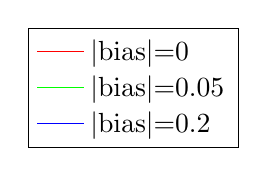
\begin{tikzpicture}
  \begin{customlegend}[legend entries={
        \textbar bias\textbar=0,
        \textbar bias\textbar=0.05,
        \textbar bias\textbar=0.2
      },
      legend cell align=left
    ]
    \addlegendimage{no markers,red}
    \addlegendimage{no markers,green}
    \addlegendimage{no markers,blue}
    \end{customlegend}
\end{tikzpicture}
}
                \caption{Legend}

        \end{subfigure}%
        \begin{subfigure}[b]{0.5\columnwidth}
                \resizebox{\columnwidth}{!}{% This file was created by matlab2tikz.
% Minimal pgfplots version: 1.3
%
%The latest updates can be retrieved from
%  http://www.mathworks.com/matlabcentral/fileexchange/22022-matlab2tikz
%where you can also make suggestions and rate matlab2tikz.
%
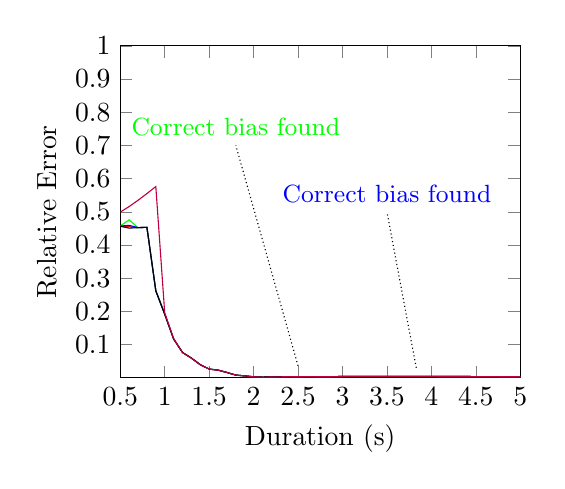
\begin{tikzpicture}

\begin{axis}[%
width= 2in,
height=1.66in,
at={(1.748842in,1.091895in)},
scale only axis,
xmin=0.5,
xmax=5,
xlabel={Duration (s)},
ytick={0.1,0.2,...,1,1.1},
xtick={0.5,1,...,4.5,5},
ymin=0,
ymax=1,
ylabel={Relative Error},
legend style={legend cell align=left,align=left,draw=white!15!black}
]
\addplot [color=red]
  table[row sep=crcr]{%
0.5	0.457213302127421\\
0.6	0.455192341479604\\
0.7	0.452216037796734\\
0.8	0.453190103081673\\
0.9	0.261969141828324\\
1	0.191825188870578\\
1.1	0.117095165791044\\
1.2	0.0762768380845627\\
1.3	0.0594633596512918\\
1.4	0.039516578981944\\
1.5	0.0262860927366302\\
1.6	0.0231175232086304\\
1.7	0.0160171848222492\\
1.8	0.00806571971450486\\
1.9	0.00570566212280324\\
2	0.00308870167452464\\
2.1	0.00211821097852379\\
2.2	0.00256398237455305\\
2.3	0.00302351761662976\\
2.4	0.00350985453723566\\
2.5	0.00314065425000658\\
2.6	0.00351257288379752\\
2.7	0.00332479648971595\\
2.8	0.00305225382986762\\
2.9	0.00340745854763594\\
3	0.00404089700549786\\
3.1	0.0042407211270089\\
3.2	0.00417814064758956\\
3.3	0.00415926826096143\\
3.4	0.00419653337493834\\
3.5	0.00420249592927426\\
3.6	0.0043182710908231\\
3.7	0.00428540620480067\\
3.8	0.0044069241030255\\
3.9	0.00428007958863001\\
4	0.00414948546341961\\
4.1	0.00401503224617003\\
4.2	0.00389550043709871\\
4.3	0.00377267435550791\\
4.4	0.00376475729829568\\
4.5	0.00364761408625085\\
4.6	0.00357675042647449\\
4.7	0.00337183649599589\\
4.8	0.0032520645794267\\
4.9	0.00310724581166637\\
5	0.00301680980763474\\
  };

  \addplot [color=green]
  table[row sep=crcr]{%
0.5	0.457156144374328\\
0.6	0.475568507249425\\
0.7	0.452216526751907\\
0.8	0.453184216720428\\
0.9	0.261970927264874\\
1	0.191824149736225\\
1.1	0.117094877791212\\
1.2	0.0762766834804991\\
1.3	0.0594632845267134\\
1.4	0.0395165388185115\\
1.5	0.0262860684107174\\
1.6	0.0231175211446198\\
1.7	0.01601777515452\\
1.8	0.00806620230597057\\
1.9	0.00570585002306924\\
2	0.00308878993518567\\
2.1	0.00211826133527056\\
2.2	0.00256407572117813\\
2.3	0.00302353310334371\\
2.4	0.00350986535474506\\
2.5	0.00314066271579074\\
2.6	0.00351257656781648\\
2.7	0.00332479212486378\\
2.8	0.00305224906749911\\
2.9	0.00340746234454352\\
3	0.00404090552310241\\
3.1	0.00424073652149371\\
3.2	0.00417816095801413\\
3.3	0.00415929728394695\\
3.4	0.00419652664123642\\
3.5	0.00420249041481522\\
3.6	0.00431826604113076\\
3.7	0.00428540188160041\\
3.8	0.00440692004851839\\
3.9	0.00428007686253398\\
4	0.00414948305784513\\
4.1	0.00401502795135146\\
4.2	0.00389549763257924\\
4.3	0.00377270572221868\\
4.4	0.00376478652037804\\
4.5	0.00364763560171335\\
4.6	0.00357676733533996\\
4.7	0.00337184737487797\\
4.8	0.00325207527835561\\
4.9	0.00310725663112416\\
5	0.00301681702941922\\
  };

  \addplot [color=blue]
  table[row sep=crcr]{%
0.5	0.457075629147129\\
0.6	0.459090047905311\\
0.7	0.452217510595409\\
0.8	0.453285771870529\\
0.9	0.261979808590916\\
1	0.191823826022661\\
1.1	0.117094774096814\\
1.2	0.0762766418196225\\
1.3	0.0594632493852891\\
1.4	0.0395164711160309\\
1.5	0.0262860031082735\\
1.6	0.0231174747227512\\
1.7	0.0160177423686259\\
1.8	0.00806618238060448\\
1.9	0.00570583868247728\\
2	0.00308878046798837\\
2.1	0.00211825777140346\\
2.2	0.00256407955301464\\
2.3	0.00302354466859032\\
2.4	0.00350987945044755\\
2.5	0.00314067604182949\\
2.6	0.00351258938406874\\
2.7	0.00332480197595684\\
2.8	0.00305225604421829\\
2.9	0.00340746684019399\\
3	0.00404090878142968\\
3.1	0.00424073727160898\\
3.2	0.00417816074077772\\
3.3	0.00415929523007111\\
3.4	0.00419652354515818\\
3.5	0.0042024863319461\\
3.6	0.00431826101006045\\
3.7	0.00428539653764112\\
3.8	0.00440691344735517\\
3.9	0.0042800706957711\\
4	0.00414947667179806\\
4.1	0.00401502231692606\\
4.2	0.00389549120801378\\
4.3	0.00377269895695827\\
4.4	0.00376478057935468\\
4.5	0.00364762892783341\\
4.6	0.00357676023236904\\
4.7	0.00337183894820681\\
4.8	0.00325206823888659\\
4.9	0.00310724913012118\\
5	0.00301680919544336\\
  };

  \addplot [color=black]
  table[row sep=crcr]{%
0.5	0.456389016891691\\
0.6	0.450813616771932\\
0.7	0.452216282826301\\
0.8	0.453275696548976\\
0.9	0.261915465666417\\
1	0.191823000225505\\
1.1	0.117097207037816\\
1.2	0.0762772496901397\\
1.3	0.0594633109536488\\
1.4	0.0395164091005799\\
1.5	0.026285827668707\\
1.6	0.0231173216282823\\
1.7	0.0160175969352111\\
1.8	0.00806600990655503\\
1.9	0.00570567459847116\\
2	0.00308856820691083\\
2.1	0.00211804996139152\\
2.2	0.00256388047700766\\
2.3	0.00302345079693929\\
2.4	0.00350981717362306\\
2.5	0.00314062234513454\\
2.6	0.00351255913155156\\
2.7	0.00332478122272159\\
2.8	0.00305223939546943\\
2.9	0.00340746273618067\\
3	0.00404091698988087\\
3.1	0.00424071665805606\\
3.2	0.00417814127253803\\
3.3	0.00415927642175141\\
3.4	0.00419650568413711\\
3.5	0.00420246881349827\\
3.6	0.00431824414113396\\
3.7	0.0042853801840044\\
3.8	0.00440689913756316\\
3.9	0.00428005441756171\\
4	0.00414945956304029\\
4.1	0.00401500622106869\\
4.2	0.0038954732662318\\
4.3	0.00377268135515568\\
4.4	0.00376476119133187\\
4.5	0.00364760922742163\\
4.6	0.00357673945042915\\
4.7	0.00337181811409821\\
4.8	0.00325204490236603\\
4.9	0.00310722504952145\\
5	0.00301678429841179\\
  };

  \addplot [color=purple]
  table[row sep=crcr]{%
0.5	0.498937913290902\\
0.6	0.515806914699162\\
0.7	0.534604096568107\\
0.8	0.554841088919843\\
0.9	0.575996329819569\\
1	0.196136294912996\\
1.1	0.118158003685231\\
1.2	0.0760968925741495\\
1.3	0.0588983950730206\\
1.4	0.0390879885857865\\
1.5	0.02612190252608\\
1.6	0.0230033286211537\\
1.7	0.0160000046691293\\
1.8	0.00807552424272596\\
1.9	0.00568304066315242\\
2	0.00301648092492872\\
2.1	0.00198246699936726\\
2.2	0.00236734269949844\\
2.3	0.00286857079015789\\
2.4	0.00337456976760228\\
2.5	0.00301590078457125\\
2.6	0.00339807554012536\\
2.7	0.00321960523676702\\
2.8	0.00294994604944067\\
2.9	0.00331651777287667\\
3	0.00395863533844159\\
3.1	0.00416509907024152\\
3.2	0.00410757843001639\\
3.3	0.00409528823099574\\
3.4	0.004136737207005\\
3.5	0.00414792686718712\\
3.6	0.00426775398151668\\
3.7	0.00423846273323052\\
3.8	0.00436207103792608\\
3.9	0.00424007616111341\\
4	0.0041141284578057\\
4.1	0.00398200278291087\\
4.2	0.00386583326889654\\
4.3	0.0037452157159102\\
4.4	0.00373849057682891\\
4.5	0.00362285993112944\\
4.6	0.0035536327550714\\
4.7	0.00334976952192879\\
4.8	0.00323087770921777\\
4.9	0.00308748602337737\\
5	0.00299952588920156\\
  };

  \draw[densely dotted] (axis cs:2.5,0.036) -- (axis cs:1.8,0.7) node [above] {\color{green}\small Correct bias found};

%% \addlegendentry{\textbar bias\textbar =0.2};
\draw[densely dotted] (axis cs:3.83,0.03) -- (axis cs:3.5,0.5) node [above] {\color{blue}\small Correct bias found};


\end{axis}
\end{tikzpicture}%
}
                \caption{Gravity estimation error}

        \end{subfigure}
        ~
        \begin{subfigure}[b]{0.5\columnwidth}
                \resizebox{\columnwidth}{!}{% This file was created by matlab2tikz.
% Minimal pgfplots version: 1.3
%
%The latest updates can be retrieved from
%  http://www.mathworks.com/matlabcentral/fileexchange/22022-matlab2tikz
%where you can also make suggestions and rate matlab2tikz.
%
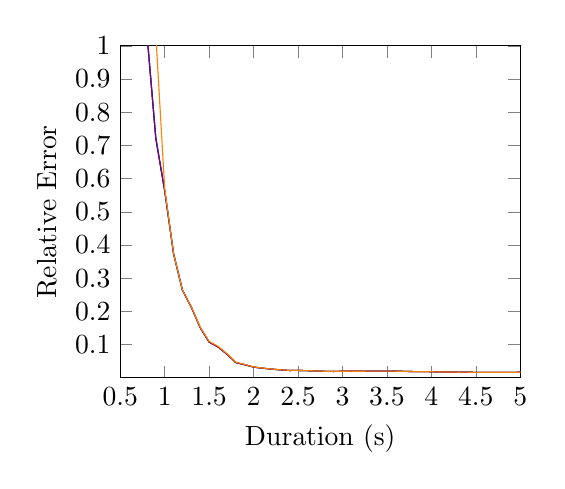
\begin{tikzpicture}

\begin{axis}[%
width= 2in,
height=1.66in,
at={(1.751579in,1.09421in)},
scale only axis,
xmin=0.5,
xmax=5,
xlabel={Duration (s)},
ytick={0.1,0.2,...,1,1.1},
xtick={0.5,1,...,4.5,5},
ymin=0,
ymax=1,
ylabel={Relative Error},
legend style={legend cell align=left,align=left,draw=white!15!black}
]
\addplot [color=red]
  table[row sep=crcr]{%
0.5	1.03428842951012\\
0.6	1.03638271644628\\
0.7	1.03705622686708\\
0.8	1.0370242651449\\
0.9	0.721460329228353\\
1	0.563322442418376\\
1.1	0.373266033741862\\
1.2	0.263598510570558\\
1.3	0.212244884847796\\
1.4	0.150642868840018\\
1.5	0.107477474988098\\
1.6	0.0928771698398517\\
1.7	0.0711655323548572\\
1.8	0.0459349012433474\\
1.9	0.0393061778689527\\
2	0.0322091669303359\\
2.1	0.0288520802594844\\
2.2	0.0261319200649033\\
2.3	0.0238985726343984\\
2.4	0.0220916756573955\\
2.5	0.0221686815876314\\
2.6	0.0214786648755916\\
2.7	0.0206480989006068\\
2.8	0.0194911656100721\\
2.9	0.0190559168108787\\
3	0.0197565637669144\\
3.1	0.019910593262248\\
3.2	0.0195863285299865\\
3.3	0.0201131659325989\\
3.4	0.0199213813257751\\
3.5	0.0200115735490841\\
3.6	0.0199431908448099\\
3.7	0.0193642927180046\\
3.8	0.0186935972613029\\
3.9	0.0187148921256151\\
4	0.0182275142784112\\
4.1	0.0175588126898573\\
4.2	0.0175492113139643\\
4.3	0.0168146469704028\\
4.4	0.0169632511859468\\
4.5	0.0162567546355651\\
4.6	0.0162939068936979\\
4.7	0.016272652084721\\
4.8	0.0163987585563958\\
4.9	0.0163557587533478\\
5	0.0165962225460581\\
  };

\addplot [color=green]
  table[row sep=crcr]{%
0.5	1.03431921033724\\
0.6	1.02847462118116\\
0.7	1.03705584840796\\
0.8	1.03705155448565\\
0.9	0.721464220160781\\
1	0.563320096490998\\
1.1	0.373265378852485\\
1.2	0.263598184706692\\
1.3	0.212244780744222\\
1.4	0.15064287224147\\
1.5	0.107477539984016\\
1.6	0.0928772902687234\\
1.7	0.071166819391878\\
1.8	0.045935439101605\\
1.9	0.0393063876899866\\
2	0.0322092686665937\\
2.1	0.0288521760366202\\
2.2	0.026132011155991\\
2.3	0.0238986219471569\\
2.4	0.0220916972767572\\
2.5	0.0221687175328368\\
2.6	0.0214786940028647\\
2.7	0.0206481365038836\\
2.8	0.0194911948143448\\
2.9	0.0190559411727344\\
3	0.0197565846493807\\
3.1	0.019910611166176\\
3.2	0.0195863502588877\\
3.3	0.020113195546417\\
3.4	0.0199213715520477\\
3.5	0.0200115627751808\\
3.6	0.0199431772984777\\
3.7	0.0193642780438425\\
3.8	0.0186935824405396\\
3.9	0.0187148797358102\\
4	0.0182275008965334\\
4.1	0.01755879821913\\
4.2	0.0175491977265304\\
4.3	0.0168146752743008\\
4.4	0.0169632782409571\\
4.5	0.0162567731309442\\
4.6	0.0162939183302371\\
4.7	0.0162726570221423\\
4.8	0.0163987621843931\\
4.9	0.0163557588632198\\
5	0.0165962186341798\\
  };

  \addplot [color=blue]
  table[row sep=crcr]{%
0.5	1.03436202097109\\
0.6	1.03469660142723\\
0.7	1.03705537516161\\
0.8	1.03700877545863\\
0.9	0.72148359632809\\
1	0.563319273172429\\
1.1	0.373265010803895\\
1.2	0.26359794053019\\
1.3	0.212244561084914\\
1.4	0.150642592542543\\
1.5	0.107477284125723\\
1.6	0.0928770955685183\\
1.7	0.0711666754697577\\
1.8	0.0459353517993857\\
1.9	0.039306324597766\\
2	0.0322092152921413\\
2.1	0.0288521277430945\\
2.2	0.0261319675588511\\
2.3	0.0238985930024124\\
2.4	0.0220916831090088\\
2.5	0.0221687044219438\\
2.6	0.0214786865704747\\
2.7	0.0206481329107525\\
2.8	0.0194911886500881\\
2.9	0.0190559329502011\\
3	0.0197565705117338\\
3.1	0.0199105913476138\\
3.2	0.019586328463443\\
3.3	0.0201131748653326\\
3.4	0.0199213481719146\\
3.5	0.0200115386973725\\
3.6	0.019943151784345\\
3.7	0.0193642504723163\\
3.8	0.0186935481977495\\
3.9	0.0187148492432098\\
4	0.0182274738504595\\
4.1	0.0175587695077671\\
4.2	0.0175491701653304\\
4.3	0.0168146497356487\\
4.4	0.0169632533668464\\
4.5	0.0162567519540275\\
4.6	0.0162939012826876\\
4.7	0.0162726419573455\\
4.8	0.0163987504591162\\
4.9	0.0163557515661635\\
5	0.0165962187476694\\
  };

  \addplot [color=violet]
  table[row sep=crcr]{%
0.5	1.03476192547132\\
0.6	1.03758197407633\\
0.7	1.0370557226161\\
0.8	1.03701241601538\\
0.9	0.72134367164526\\
1	0.563317797927101\\
1.1	0.373269855806708\\
1.2	0.263598035273144\\
1.3	0.212244418687358\\
1.4	0.150642192051305\\
1.5	0.107476813573889\\
1.6	0.0928767783735264\\
1.7	0.0711664413039552\\
1.8	0.045935270152318\\
1.9	0.0393063171453859\\
2	0.0322093163753734\\
2.1	0.0288523015628475\\
2.2	0.0261321479631278\\
2.3	0.0238988077466903\\
2.4	0.0220918885376059\\
2.5	0.022168849078177\\
2.6	0.0214787742939537\\
2.7	0.020648207588432\\
2.8	0.0194912456057143\\
2.9	0.0190559767252324\\
3	0.0197566286318099\\
3.1	0.0199105491991258\\
3.2	0.019586284228284\\
3.3	0.0201131291780162\\
3.4	0.0199213055198734\\
3.5	0.0200114959166887\\
3.6	0.0199431118712093\\
3.7	0.0193642114290031\\
3.8	0.0186935146038441\\
3.9	0.0187148147516913\\
4	0.0182274390995322\\
4.1	0.0175587377602335\\
4.2	0.0175491383313107\\
4.3	0.016814616980133\\
4.4	0.0169632201575355\\
4.5	0.0162567164756863\\
4.6	0.0162938645039988\\
4.7	0.0162726042988577\\
4.8	0.0163987111137495\\
4.9	0.0163557101648641\\
5	0.016596174700194\\
  };

\addplot [color=orange]
  table[row sep=crcr]{%
0.5	1.01036339910637\\
0.6	1.01264609243497\\
0.7	1.01712479824903\\
0.8	1.02432857529485\\
0.9	1.03489886439788\\
1	0.569748764074271\\
1.1	0.374125042592347\\
1.2	0.263657517534064\\
1.3	0.212885819503723\\
1.4	0.152284959714533\\
1.5	0.10960916091804\\
1.6	0.09492070177218\\
1.7	0.0728050791912558\\
1.8	0.0471436644973108\\
1.9	0.0401256275926041\\
2	0.0328210601640846\\
2.1	0.0293152906350284\\
2.2	0.0264773390946265\\
2.3	0.0241800284470093\\
2.4	0.0223021071421193\\
2.5	0.0223235972550982\\
2.6	0.0215741868518377\\
2.7	0.0207099655511168\\
2.8	0.0195531091032568\\
2.9	0.0190798137289304\\
3	0.0197270218698771\\
3.1	0.0198704322232954\\
3.2	0.0195448470808233\\
3.3	0.0200757068195603\\
3.4	0.0198831591779835\\
3.5	0.0199747807834981\\
3.6	0.0199060205001915\\
3.7	0.0193281809984972\\
3.8	0.0186561503150706\\
3.9	0.0186879895121145\\
4	0.0182079673309161\\
4.1	0.0175411271077639\\
4.2	0.0175361546561091\\
4.3	0.0168049010547206\\
4.4	0.0169532300968722\\
4.5	0.0162489358167096\\
4.6	0.0162878716035583\\
4.7	0.0162687939533226\\
4.8	0.0163958472551503\\
4.9	0.01635462748761\\
5	0.0165968366730399\\
  };

  %% \draw[densely dotted] (axis cs:2.5,0.09) -- (axis cs:1.5,0.6) node [above, text width=2cm,align=center] {\color{green}\small Correct bias found};

  %% \draw[densely dotted] (axis cs:3.83,0.105) -- (axis cs:3.1,0.5) node [above, text width=2cm,align=center] {\color{blue}\small Correct bias found};



\end{axis}
\end{tikzpicture}%
}
                \caption{Velocity estimation error}

        \end{subfigure}%
        \begin{subfigure}[b]{0.5\columnwidth}
                \resizebox{\columnwidth}{!}{% This file was created by matlab2tikz.
% Minimal pgfplots version: 1.3
%
%The latest updates can be retrieved from
%  http://www.mathworks.com/matlabcentral/fileexchange/22022-matlab2tikz
%where you can also make suggestions and rate matlab2tikz.
%
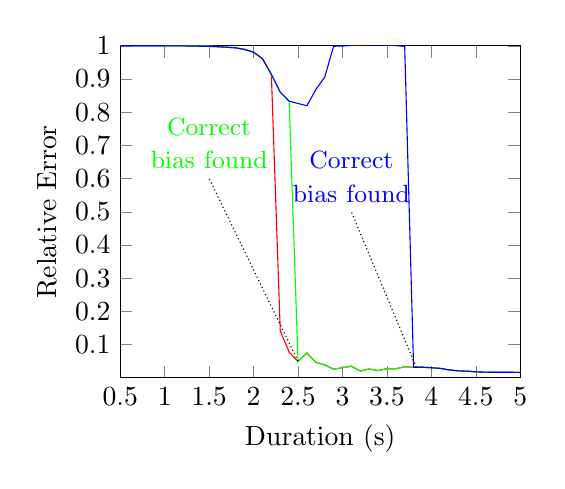
\begin{tikzpicture}

\begin{axis}[%
width= 2in,
height=1.66in,
at={(1.751579in,1.09421in)},
scale only axis,
xmin=0.5,
xmax=5,
xlabel={Duration (s)},
ytick={0.1,0.2,...,1,1.1},
xtick={0.5,1,...,4.5,5},
ymin=0,
ymax=1,
ylabel={Relative Error},
legend style={legend cell align=left,align=left,draw=white!15!black}
  ]
  \addplot [color=red,solid]
  table[row sep=crcr]{%
0.5	1.00066447949451\\
0.6	1.0000171574083\\
0.7	1.00019992642903\\
0.8	1.00004747070073\\
0.9	0.999990701475109\\
1	0.999951817654236\\
1.1	0.999892763917228\\
1.2	0.999812856315744\\
1.3	0.999218198592552\\
1.4	0.998873832391133\\
1.5	0.998408657943417\\
1.6	0.997199887802298\\
1.7	0.99559817356649\\
1.8	0.993824576708259\\
1.9	0.988863534885469\\
2	0.980741806020155\\
2.1	0.961096823210096\\
2.2	0.913582611330772\\
2.3	0.14165838947277\\
2.4	0.077319529238396\\
2.5	0.0491173169352688\\
2.6	0.0748693564361423\\
2.7	0.0465915300523226\\
2.8	0.0387705637335366\\
2.9	0.0258643583533819\\
3	0.0303941591921433\\
3.1	0.0349664749284648\\
3.2	0.0202805690730165\\
3.3	0.0265636795136452\\
3.4	0.0215510398530458\\
3.5	0.0273062350214222\\
3.6	0.0272218054025453\\
3.7	0.0331354880624203\\
3.8	0.0315417398987069\\
3.9	0.0318444092048247\\
4	0.0302012330036885\\
4.1	0.02837093980372\\
4.2	0.0237425212726591\\
4.3	0.0209382612828654\\
4.4	0.019956686849123\\
4.5	0.0178642105653145\\
4.6	0.0170389988338836\\
4.7	0.0165804975572116\\
4.8	0.0165186409622677\\
4.9	0.0166359748752942\\
5	0.0159729227243361\\
};
%% \addlegendentry{\textbar bias\textbar =0};

\addplot [color=green,solid]
  table[row sep=crcr]{%
0.5	1.00044900448995\\
0.6	1.00002183673998\\
0.7	1.00013755704372\\
0.8	1.00005327640927\\
0.9	0.99996880953275\\
1	0.999904893086687\\
1.1	0.999776871222249\\
1.2	0.999809912820316\\
1.3	0.999655325831441\\
1.4	0.999524380520714\\
1.5	0.99926056513569\\
1.6	0.997369846269512\\
1.7	0.995623493639254\\
1.8	0.993826487702919\\
1.9	0.988872496376655\\
2	0.980745491897591\\
2.1	0.961072056402476\\
2.2	0.913618087829766\\
2.3	0.85993902980691\\
2.4	0.832542568716734\\
2.5	0.0491245780239571\\
2.6	0.0748625739833272\\
2.7	0.0465435229598398\\
2.8	0.0387705769336132\\
2.9	0.025859356022133\\
3	0.030390194572122\\
3.1	0.0349691928653105\\
3.2	0.0202819014894071\\
3.3	0.0265669147665207\\
3.4	0.0215521246469244\\
3.5	0.0273070924255307\\
3.6	0.0272226364858804\\
3.7	0.0331361610578156\\
3.8	0.0315421975818471\\
3.9	0.0318447329758112\\
4	0.0302013872766145\\
4.1	0.0283710435884954\\
4.2	0.0237424853348519\\
4.3	0.0209381315115916\\
4.4	0.019956449864681\\
4.5	0.0178638925462151\\
4.6	0.0170384537509053\\
4.7	0.0165798671335275\\
4.8	0.0165179805639359\\
4.9	0.0166353863605497\\
5	0.0159724545914235\\
};
%% \addlegendentry{\textbar bias\textbar =0.05};
\addplot [color=blue,solid]
  table[row sep=crcr]{%
0.5	1.00005587186573\\
0.6	0.999994927395622\\
0.7	1.00019014775547\\
0.8	1.00000397951626\\
0.9	0.9999897444568\\
1	0.999937598975941\\
1.1	0.999740738719758\\
1.2	0.999816328191023\\
1.3	0.999042986366212\\
1.4	0.998702441136465\\
1.5	0.998252386497607\\
1.6	0.997094396229848\\
1.7	0.995571374932069\\
1.8	0.993794704995225\\
1.9	0.988871396346665\\
2	0.980760795391842\\
2.1	0.96117613864454\\
2.2	0.914342082246868\\
2.3	0.860571829647345\\
2.4	0.83309501298875\\
2.5	0.826159267466917\\
2.6	0.819616033495059\\
2.7	0.867983017844418\\
2.8	0.90528456633506\\
2.9	0.998594108003211\\
3	0.999253777359576\\
3.1	1.00090793996248\\
3.2	1.00189038650018\\
3.3	1.00253837305961\\
3.4	1.00273552089462\\
3.5	1.00217202066438\\
3.6	1.00064555110224\\
3.7	0.998081945874475\\
3.8	0.0315430127407853\\
3.9	0.0318452625794558\\
4	0.0302019648488514\\
4.1	0.028370825133817\\
4.2	0.0237424324349308\\
4.3	0.0209387269335419\\
4.4	0.0199566901640943\\
4.5	0.0178641675756711\\
4.6	0.017038210941125\\
4.7	0.0165801771915695\\
4.8	0.0165185092595819\\
4.9	0.0166359091919561\\
5	0.015972851633287\\
};
%% \addlegendentry{\textbar bias\textbar =0.5};

%% \draw (axis cs:3,0.0752277087348034) -- (axis cs:3,0.365) node [right] {Correct bias found};
  \draw[densely dotted] (axis cs:2.5,0.05) -- (axis cs:1.5,0.6) node [above, text width=2cm,align=center] {\color{green}\small Correct bias found};

  \draw[densely dotted] (axis cs:3.83,0.0315) -- (axis cs:3.1,0.5) node [above, text width=2cm, align=center] {\color{blue}\small Correct bias found};


\end{axis}
\end{tikzpicture}%
}
                \caption{Lambda estimation error}

        \end{subfigure}
        \caption{Impact of the gyroscope bias on the performance of the optimized closed-form solution. We are observing 7 features  over a variable duration of integration. \label{fig:biasGyroOpt}}
\end{figure}

\begin{figure}
  \centering
  \resizebox{0.7\columnwidth}{!}{% This file was created by matlab2tikz.
% Minimal pgfplots version: 1.3
%
%The latest updates can be retrieved from
%  http://www.mathworks.com/matlabcentral/fileexchange/22022-matlab2tikz
%where you can also make suggestions and rate matlab2tikz.
%
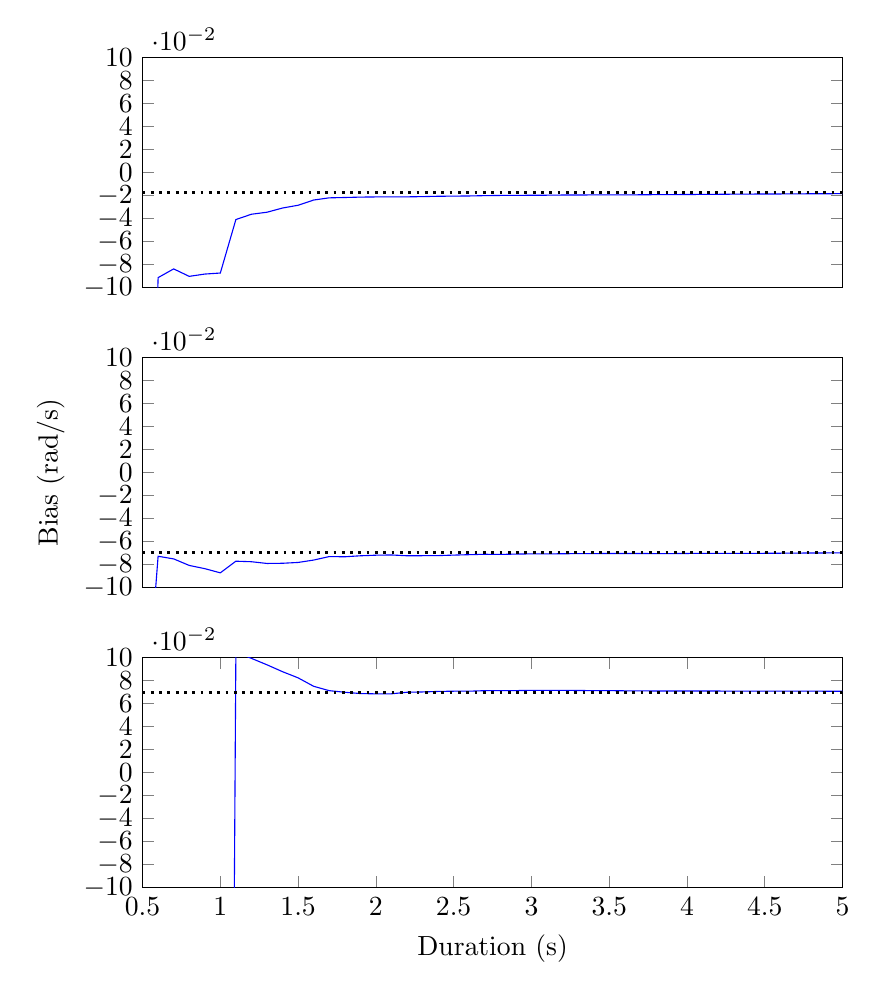
\begin{tikzpicture}

\begin{axis}[%
width=3.5in,
height=1.15in,
at={(0in,3in)},
scale only axis,
xmin=0.5,
xmax=5,
scaled y ticks={base 10:2},
ytick={-0.1, -0.08, -0.06, -0.04,-0.02,0,0.02,0.04,0.06,0.08,0.1},
ymin=-0.1,
ymax=0.1,
xmajorticks=false
]
\addplot [color=blue,solid,forget plot]
  table[row sep=crcr]{%
0.5	-0.613719530125534\\
0.6	-0.0912928634245716\\
0.7	-0.0836974439106333\\
0.8	-0.0901824533724056\\
0.9	-0.0881937603605537\\
1	-0.0872925176140616\\
1.1	-0.0407906270864024\\
1.2	-0.0361672813730119\\
1.3	-0.0344206231212715\\
1.4	-0.0307633937803476\\
1.5	-0.0283536037134608\\
1.6	-0.0238128480391266\\
1.7	-0.0219100166095823\\
1.8	-0.0216152331488808\\
1.9	-0.0212697052395253\\
2	-0.0211189299014744\\
2.1	-0.0210481529500256\\
2.2	-0.021046779870389\\
2.3	-0.020845749809941\\
2.4	-0.0205395433078229\\
2.5	-0.0204173609527179\\
2.6	-0.0202818719417482\\
2.7	-0.0199945027235829\\
2.8	-0.0198239152596968\\
2.9	-0.0197970583446156\\
3	-0.0196430113620259\\
3.1	-0.0196101346524373\\
3.2	-0.0194721192783091\\
3.3	-0.0194745679539277\\
3.4	-0.0193375774834139\\
3.5	-0.0193451092133124\\
3.6	-0.019327911377094\\
3.7	-0.0192582557689741\\
3.8	-0.0191436748398716\\
3.9	-0.0190836100504351\\
4	-0.0190233026232585\\
4.1	-0.0189116627347921\\
4.2	-0.018842430071302\\
4.3	-0.0187056680462616\\
4.4	-0.0186479140535241\\
4.5	-0.0185547484869255\\
4.6	-0.018529463993065\\
4.7	-0.0184401786869746\\
4.8	-0.0183765940813847\\
4.9	-0.0183124596306187\\
5	-0.0182965427990539\\
};
\draw[line width=1pt, dotted]  (axis cs: 0.5, -0.0170 ) -- (axis cs:5., -0.0170);

\end{axis}





\begin{axis}[%
width=3.5in,
height=1.15in,
at={(0in,1.5in)},
scale only axis,
xmin=0.5,
xmax=5,
scaled y ticks={base 10:2},
ytick={-0.1, -0.08, -0.06, -0.04,-0.02,0,0.02,0.04,0.06,0.08,0.1},
ymin=-0.1,
ymax=0.1,
xmajorticks=false,
ylabel={Bias (rad/s)}
]
\addplot [color=blue,solid,forget plot]
  table[row sep=crcr]{%
0.5	-0.249123077995011\\
0.6	-0.0727233477080182\\
0.7	-0.0749915623266901\\
0.8	-0.0806778888517085\\
0.9	-0.0834831824853637\\
1	-0.0871177671571807\\
1.1	-0.077001932989438\\
1.2	-0.0774572301216456\\
1.3	-0.0789722506826707\\
1.4	-0.0788088184158987\\
1.5	-0.0780867520452622\\
1.6	-0.0760166452772171\\
1.7	-0.0729750701668396\\
1.8	-0.073155533427756\\
1.9	-0.0722971229579253\\
2	-0.0717838953310039\\
2.1	-0.0715817417914045\\
2.2	-0.0722732710221088\\
2.3	-0.0722152426367215\\
2.4	-0.0721347556212073\\
2.5	-0.0717050622555761\\
2.6	-0.0713332143308226\\
2.7	-0.0709806152583301\\
2.8	-0.0711175039432865\\
2.9	-0.0708234282057126\\
3	-0.0706279743404952\\
3.1	-0.0706363827827937\\
3.2	-0.0705334996652266\\
3.3	-0.0704047509045599\\
3.4	-0.0704253388704617\\
3.5	-0.0702950810601142\\
3.6	-0.0703034644071306\\
3.7	-0.0702617202834492\\
3.8	-0.0704513457281704\\
3.9	-0.0703844379039927\\
4	-0.0702621859289546\\
4.1	-0.070249562021298\\
4.2	-0.070160769597811\\
4.3	-0.0701424495796041\\
4.4	-0.0701689299930106\\
4.5	-0.0701343810370672\\
4.6	-0.0700465930666792\\
4.7	-0.0699427976687786\\
4.8	-0.0698883658184649\\
4.9	-0.0698188738421954\\
5	-0.0697149604199584\\
};
\draw[line width=1pt, dotted]  (axis cs: 0.5, -0.0695 ) -- (axis cs:5., -0.0695);
\end{axis}

\begin{axis}[%
width=3.5in,
height=1.15in,
at={(0in,0in)},
scale only axis,
xmin=0.5,
xmax=5,
xlabel={Duration (s)},
scaled y ticks={base 10:2},
ytick={-0.1, -0.08, -0.06, -0.04,-0.02,0,0.02,0.04,0.06,0.08,0.1},
ymin=-0.1,
ymax=0.1,
xtick={0.5, 1,..., 4.5, 5}
]
\addplot [color=blue,solid,forget plot]
  table[row sep=crcr]{%
0.5	-0.732634365292344\\
0.6	-1.98557179128582\\
0.7	-2.00095264239806\\
0.8	-1.98927527437268\\
0.9	-1.99396078800386\\
1	-1.99467556489905\\
1.1	0.104780731231241\\
1.2	0.0993526416647996\\
1.3	0.0937538690884356\\
1.4	0.0877633815158083\\
1.5	0.082407961499653\\
1.6	0.0750629498593657\\
1.7	0.0712684342923801\\
1.8	0.0698905861520058\\
1.9	0.0687623270994058\\
2	0.0684877397930655\\
2.1	0.0685304599950853\\
2.2	0.069880381940671\\
2.3	0.0701486197811293\\
2.4	0.0706025158524518\\
2.5	0.070804524879665\\
2.6	0.0708072124495772\\
2.7	0.0712670246415531\\
2.8	0.0712460640915076\\
2.9	0.0713274127376781\\
3	0.0715291343329739\\
3.1	0.0715729050955214\\
3.2	0.071524879408994\\
3.3	0.0714223768597761\\
3.4	0.0712945402149279\\
3.5	0.0712984512382853\\
3.6	0.0711335005885556\\
3.7	0.071066397282806\\
3.8	0.070996852064375\\
3.9	0.0710134062572396\\
4	0.0709422589555251\\
4.1	0.0709665823959415\\
4.2	0.0709335172220389\\
4.3	0.0708903967299732\\
4.4	0.0708360570734978\\
4.5	0.0708078121438934\\
4.6	0.0708088576642803\\
4.7	0.0708156486405341\\
4.8	0.0708474229075585\\
4.9	0.0707861364383358\\
5	0.0707519442192118\\
};
  \draw[line width=1pt, dotted]  (axis cs: 0.5, 0.0698 ) -- (axis cs:5., 0.0698);
\end{axis}

\end{tikzpicture}%
}
  \caption{Gyroscope bias estimation from nonlinear minimization of the residual.
    We are observing 7 features over a variable duration of integration.
    The true bias is $B=[-0.0170, -0.0695, 0.0698]$ with magnitude $||B||=0.1$ and the final bias estimate is $[-0.0183, -0.0697, 0.0708]$.\label{fig:gBiasEstimate}}
\end{figure}

%% This technique is similar to the one used in \cite{Abbeel2005}, where the author minimizes the residual of a Kalman filter in order to recover the noise matrix for the sensors.

%% Moreover, the optimized closed-form solution requires a shorter integration duration to provide good quality results.
%% Specifically, after 2 seconds of integration (around 7 frames) the provided estimations are already robust.
%% The non-optimized closed-form solution requires 3 seconds of integration before converging to acceptable estimations.


As seen in Fig. \ref{fig:gBiasEstimate}, this method can robustly estimate high values of the gyroscope bias (relative error of final bias estimate is below $2\%$).
Fig. \ref{fig:biasGyroOpt} displays the performance of the proposed method in estimating speed, gravity in the local frame, and distances to the features in presence of the same artificial gyroscope bias from Fig. \ref{fig:biasGyroCF}.
As seen in Fig. \ref{fig:biasGyroOpt}, after $1s$ of integration duration, the estimations agree no matter how high the bias is.
In other words, given that the integration duration is long enough, this method is unaffected by the gyroscope bias.
Using Levenberg-Marquardt algorithm, the optimization process reaches its optimal value after around $4$ iterations and $20$ evaluations of the cost function.
Evaluating the cost function is equivalent to solving the linear system described in Equation (\ref{eq:mat1}).

\noindent For very short time of integration ($<1$ second), the cost function loses its local convexity and the proposed method can fail by providing a gyroscope bias much larger than the correct one.
To understand this misestimation, in Fig. \ref{fig:cost} we plot the residual with respect to the bias, which is the cost function we are minimizing.
We highlight a misestimation of the gyroscope bias by setting the duration of integration to 1 second while observing 7 features.
We refer to the components of the gyroscope bias by $B = [B_x, B_y, B_z]$.
As we can see in Fig. \ref{fig:cost}, the cost function admits a symmetry with respect to $B_z$ (and consequently it is not convex).
This symmetry replicates the minima of the true gyroscope bias along $B_z$.
The optimization process can therefore diverge from the true gyroscope bias.
In the next section, we present a method to use a priori knowledge to guide the optimization process.

\begin{figure}
        \centering
        \begin{subfigure}[b]{0.489\columnwidth}
                \resizebox{\columnwidth}{!}{% This file was created by matlab2tikz.
% Minimal pgfplots version: 1.3
%
%The latest updates can be retrieved from
%  http://www.mathworks.com/matlabcentral/fileexchange/22022-matlab2tikz
%where you can also make suggestions and rate matlab2tikz.
%
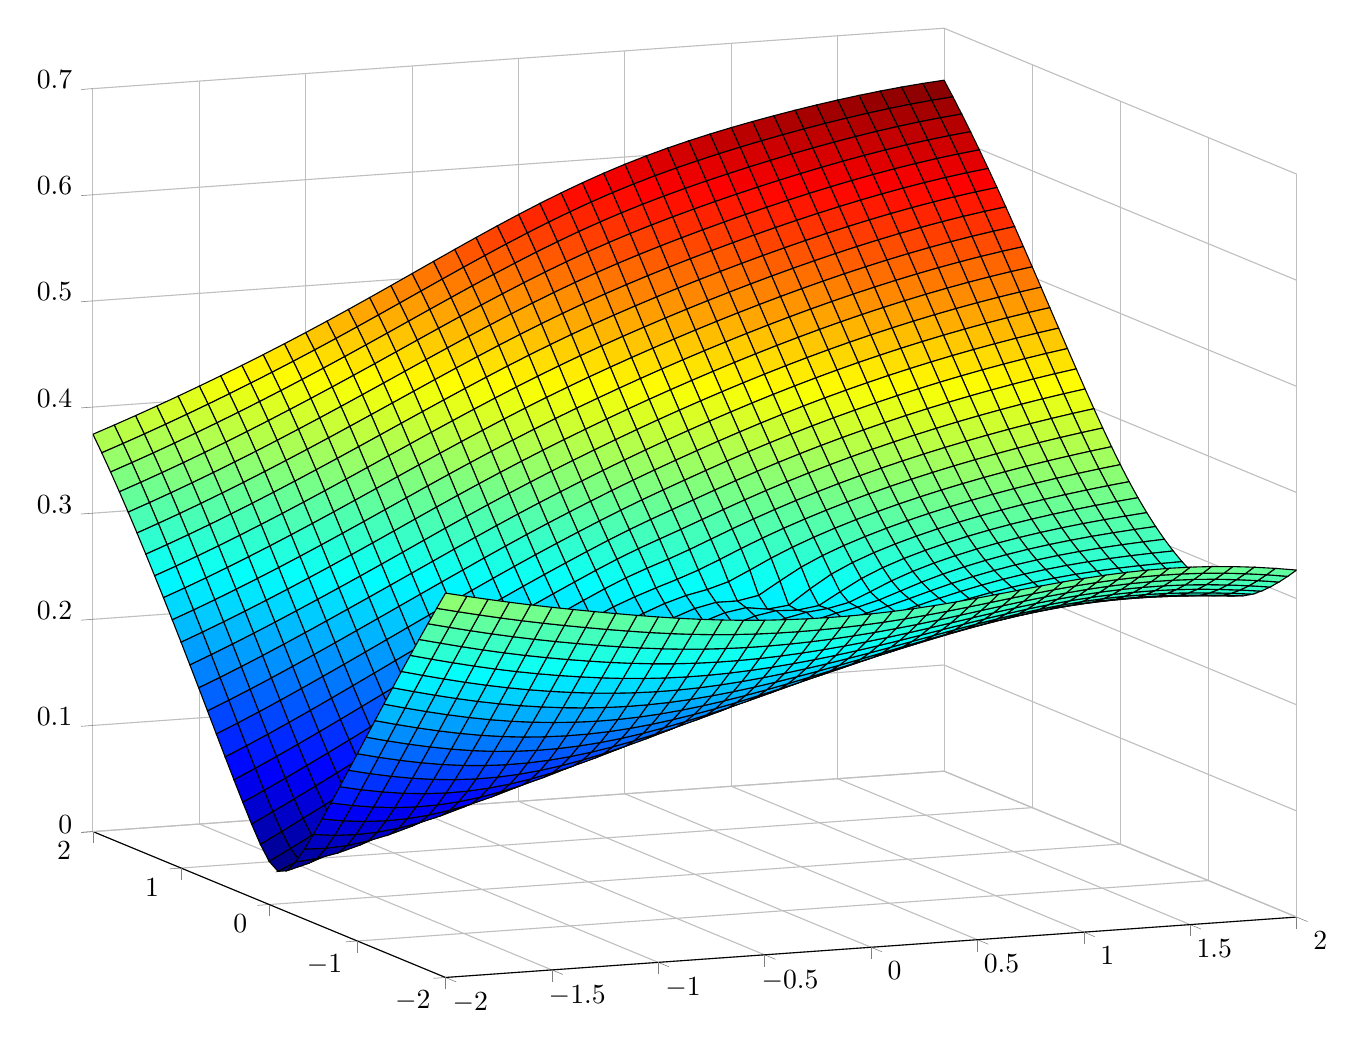
\begin{tikzpicture}

\begin{axis}[%
width=6.018285in,
height=4.74668in,
at={(1.009519in,0.640656in)},
scale only axis,
every outer x axis line/.append style={black},
every x tick label/.append style={font=\color{black}},
xmin=-2,
xmax=2,
tick align=outside,
xmajorgrids,
every outer y axis line/.append style={black},
every y tick label/.append style={font=\color{black}},
ymin=-2,
ymax=2,
ymajorgrids,
every outer z axis line/.append style={black},
every z tick label/.append style={font=\color{black}},
zmin=0,
zmax=0.7,
zmajorgrids,
view={-22.5}{12},
axis x line*=bottom,
axis y line*=left,
axis z line*=left
]

\addplot3[%
surf,
faceted color=black,
shader=faceted,
colormap/jet,
mesh/rows=41]
table[row sep=crcr,header=false] {%
%
-2	-2	0.362137849417625\\
-2	-1.9	0.34440919579571\\
-2	-1.8	0.326412846659392\\
-2	-1.7	0.30818135039005\\
-2	-1.6	0.289744193317732\\
-2	-1.5	0.271129210532984\\
-2	-1.4	0.252364171270979\\
-2	-1.3	0.233478204617797\\
-2	-1.2	0.214502888431444\\
-2	-1.1	0.19547308754338\\
-2	-1	0.176427941151522\\
-2	-0.9	0.157412756170652\\
-2	-0.8	0.138483100621946\\
-2	-0.7	0.119713553088834\\
-2	-0.6	0.101216559254465\\
-2	-0.5	0.0831852071520539\\
-2	-0.4	0.0659986700957116\\
-2	-0.3	0.0505043335555534\\
-2	-0.2	0.0387403710019821\\
-2	-0.0999999999999999	0.0346656262543176\\
-2	0	0.0405973782351522\\
-2	0.0999999999999999	0.0532388202195248\\
-2	0.2	0.0689499784777845\\
-2	0.3	0.0860261727453892\\
-2	0.4	0.103759756612721\\
-2	0.5	0.121829484571202\\
-2	0.6	0.140069342290885\\
-2	0.7	0.158376747308748\\
-2	0.8	0.176665069692588\\
-2	0.9	0.194833730282685\\
-2	1	0.212777472443026\\
-2	1.1	0.230448544047687\\
-2	1.2	0.247867616237057\\
-2	1.3	0.265047237582898\\
-2	1.4	0.281955687426331\\
-2	1.5	0.298535727480169\\
-2	1.6	0.314723866547976\\
-2	1.7	0.330457907140242\\
-2	1.8	0.345679098497999\\
-2	1.9	0.36033309055207\\
-2	2	0.374370957799394\\
-1.9	-2	0.357692610281526\\
-1.9	-1.9	0.339788224840598\\
-1.9	-1.8	0.321641069034997\\
-1.9	-1.7	0.303288093124495\\
-1.9	-1.6	0.284761773354661\\
-1.9	-1.5	0.266091662325706\\
-1.9	-1.4	0.247306538040257\\
-1.9	-1.3	0.228436747282433\\
-1.9	-1.2	0.209516408685634\\
-1.9	-1.1	0.190585446714316\\
-1.9	-1	0.171691934262883\\
-1.9	-0.9	0.152895892670991\\
-1.9	-0.8	0.134276692528206\\
-1.9	-0.7	0.115948168950263\\
-1.9	-0.6	0.0980902736385757\\
-1.9	-0.5	0.0810179885167342\\
-1.9	-0.4	0.0653370535293679\\
-1.9	-0.3	0.0522822491482419\\
-1.9	-0.2	0.0441922877492335\\
-1.9	-0.0999999999999999	0.0438435938004704\\
-1.9	0	0.0513377822409621\\
-1.9	0.0999999999999999	0.0639274031056576\\
-1.9	0.2	0.0791780669888081\\
-1.9	0.3	0.0957913118887135\\
-1.9	0.4	0.113135332856502\\
-1.9	0.5	0.13088766499727\\
-1.9	0.6	0.148867690994196\\
-1.9	0.7	0.166957423671212\\
-1.9	0.8	0.185053809362078\\
-1.9	0.9	0.203037988792015\\
-1.9	1	0.220798648641072\\
-1.9	1.1	0.238311550132648\\
-1.9	1.2	0.25561807803854\\
-1.9	1.3	0.272720799661195\\
-1.9	1.4	0.289569073049149\\
-1.9	1.5	0.306093761641701\\
-1.9	1.6	0.32222586690468\\
-1.9	1.7	0.337900793196784\\
-1.9	1.8	0.353058766822148\\
-1.9	1.9	0.367645168761767\\
-1.9	2	0.381611373518299\\
-1.8	-2	0.353382388082231\\
-1.8	-1.9	0.33531100587629\\
-1.8	-1.8	0.317021366667263\\
-1.8	-1.7	0.298556878162414\\
-1.8	-1.6	0.27995545766491\\
-1.8	-1.5	0.261250775738317\\
-1.8	-1.4	0.24247460479447\\
-1.8	-1.3	0.223660013159371\\
-1.8	-1.2	0.20484500033504\\
-1.8	-1.1	0.186076348293096\\
-1.8	-1	0.167414097053496\\
-1.8	-0.9	0.148938134615653\\
-1.8	-0.8	0.130760018961581\\
-1.8	-0.7	0.11304599378099\\
-1.8	-0.6	0.0960630218067609\\
-1.8	-0.5	0.0802715340633892\\
-1.8	-0.4	0.0665039942628314\\
-1.8	-0.3	0.0562276343109541\\
-1.8	-0.2	0.0515217726281049\\
-1.8	-0.0999999999999999	0.0538116843839784\\
-1.8	0	0.0622807042254477\\
-1.8	0.0999999999999999	0.0748168297114696\\
-1.8	0.2	0.089693904751019\\
-1.8	0.3	0.105897034601697\\
-1.8	0.4	0.122872251251348\\
-1.8	0.5	0.140309544164898\\
-1.8	0.6	0.158022841783396\\
-1.8	0.7	0.175883698171352\\
-1.8	0.8	0.193774399977933\\
-1.8	0.9	0.211557704120667\\
-1.8	1	0.22912162520455\\
-1.8	1.1	0.246475088488092\\
-1.8	1.2	0.263673788089479\\
-1.8	1.3	0.280699154717654\\
-1.8	1.4	0.297479939535519\\
-1.8	1.5	0.313937508419385\\
-1.8	1.6	0.329999358756524\\
-1.8	1.7	0.345599552627181\\
-1.8	1.8	0.360677810831769\\
-1.8	1.9	0.375179564171385\\
-1.8	2	0.389056786769167\\
-1.7	-2	0.349260378962054\\
-1.7	-1.9	0.331040592304122\\
-1.7	-1.8	0.312624613177439\\
-1.7	-1.7	0.294063688262069\\
-1.7	-1.6	0.275403664300962\\
-1.7	-1.5	0.256685574236957\\
-1.7	-1.4	0.237947566354424\\
-1.7	-1.3	0.219228385441675\\
-1.7	-1.2	0.200572317752427\\
-1.7	-1.1	0.182035344467002\\
-1.7	-1	0.163692676557367\\
-1.7	-0.9	0.145649182969162\\
-1.7	-0.8	0.128056534970234\\
-1.7	-0.7	0.111144395748074\\
-1.7	-0.6	0.0952782894259449\\
-1.7	-0.5	0.0810619767608935\\
-1.7	-0.4	0.0694864013024184\\
-1.7	-0.3	0.0620047211567604\\
-1.7	-0.2	0.0601132654565447\\
-1.7	-0.0999999999999999	0.0642564227427114\\
-1.7	0	0.073373935725798\\
-1.7	0.0999999999999999	0.0858567533363013\\
-1.7	0.2	0.100424086269916\\
-1.7	0.3	0.116265032620163\\
-1.7	0.4	0.132897007151269\\
-1.7	0.5	0.150029306112597\\
-1.7	0.6	0.167476771394569\\
-1.7	0.7	0.185104537742839\\
-1.7	0.8	0.202781573528765\\
-1.7	0.9	0.220352179129241\\
-1.7	1	0.237712619802884\\
-1.7	1.1	0.254914750467236\\
-1.7	1.2	0.272015083571378\\
-1.7	1.3	0.288963495084405\\
-1.7	1.4	0.305669976925711\\
-1.7	1.5	0.322049973789984\\
-1.7	1.6	0.33802941875644\\
-1.7	1.7	0.35354181945133\\
-1.7	1.8	0.368526701698603\\
-1.7	1.9	0.382929729750968\\
-1.7	2	0.396703681451483\\
-1.6	-2	0.345353907252555\\
-1.6	-1.9	0.327017822372578\\
-1.6	-1.8	0.308505120073981\\
-1.6	-1.7	0.289874660036091\\
-1.6	-1.6	0.271181337889115\\
-1.6	-1.5	0.252476281055027\\
-1.6	-1.4	0.233808096314525\\
-1.6	-1.3	0.215225834595661\\
-1.6	-1.2	0.196784348116851\\
-1.6	-1.1	0.178552426509938\\
-1.6	-1	0.160623945680629\\
-1.6	-0.9	0.143133128573249\\
-1.6	-0.8	0.126277458840114\\
-1.6	-0.7	0.110355315561403\\
-1.6	-0.6	0.0958277945141044\\
-1.6	-0.5	0.0834067582890431\\
-1.6	-0.4	0.0741240933995569\\
-1.6	-0.3	0.0692085594697876\\
-1.6	-0.2	0.0695426732938669\\
-1.6	-0.0999999999999999	0.0750093442903546\\
-1.6	0	0.0845779897723354\\
-1.6	0.0999999999999999	0.0970069384736958\\
-1.6	0.2	0.1113115322371\\
-1.6	0.3	0.12683144912143\\
-1.6	0.4	0.143146473762069\\
-1.6	0.5	0.159987851846337\\
-1.6	0.6	0.177175391081784\\
-1.6	0.7	0.194570785093773\\
-1.6	0.8	0.212030282471609\\
-1.6	0.9	0.229379926618252\\
-1.6	1	0.246538636491842\\
-1.6	1.1	0.263607344933732\\
-1.6	1.2	0.28062131306177\\
-1.6	1.3	0.297492789914123\\
-1.6	1.4	0.314118643672496\\
-1.6	1.5	0.330412382623143\\
-1.6	1.6	0.346299890099871\\
-1.6	1.7	0.361714549107626\\
-1.6	1.8	0.376595789744013\\
-1.6	1.9	0.390889568305553\\
-1.6	2	0.404549579875563\\
-1.5	-2	0.341655225947014\\
-1.5	-1.9	0.323247185774985\\
-1.5	-1.8	0.30468258022192\\
-1.5	-1.7	0.286026376543539\\
-1.5	-1.6	0.267341576388204\\
-1.5	-1.5	0.248689824428042\\
-1.5	-1.4	0.230132687630162\\
-1.5	-1.3	0.21173417728775\\
-1.5	-1.2	0.193565609486731\\
-1.5	-1.1	0.175714265963802\\
-1.5	-1	0.158297195117888\\
-1.5	-0.9	0.141481261446281\\
-1.5	-0.8	0.125511421312133\\
-1.5	-0.7	0.110751053504143\\
-1.5	-0.6	0.0977360099852859\\
-1.5	-0.5	0.0872245023427888\\
-1.5	-0.4	0.0801687712912531\\
-1.5	-0.3	0.0774726998484685\\
-1.5	-0.2	0.079533688529358\\
-1.5	-0.0999999999999999	0.0859669036892634\\
-1.5	0	0.0958583868301137\\
-1.5	0.0999999999999999	0.108231897872231\\
-1.5	0.2	0.122308700420935\\
-1.5	0.3	0.137542150267171\\
-1.5	0.4	0.15356533035295\\
-1.5	0.5	0.170131672095426\\
-1.5	0.6	0.18706828085941\\
-1.5	0.7	0.204235389115404\\
-1.5	0.8	0.22147621245796\\
-1.5	0.9	0.238600044293062\\
-1.5	1	0.255570598146472\\
-1.5	1.1	0.27253253337953\\
-1.5	1.2	0.289471376347398\\
-1.5	1.3	0.306264526563167\\
-1.5	1.4	0.322804159799729\\
-1.5	1.5	0.339005260182878\\
-1.5	1.6	0.354794471898391\\
-1.5	1.7	0.370105091862955\\
-1.5	1.8	0.384876355536187\\
-1.5	1.9	0.399054454041931\\
-1.5	2	0.412594020280141\\
-1.4	-2	0.338128905741597\\
-1.4	-1.9	0.319698725432507\\
-1.4	-1.8	0.301136641506603\\
-1.4	-1.7	0.28251257699143\\
-1.4	-1.6	0.263896093495239\\
-1.4	-1.5	0.245357827492212\\
-1.4	-1.4	0.226971701542536\\
-1.4	-1.3	0.208818192482163\\
-1.4	-1.2	0.190989389014469\\
-1.4	-1.1	0.173597364833097\\
-1.4	-1	0.156788233623063\\
-1.4	-0.9	0.140764241569168\\
-1.4	-0.8	0.125814768816374\\
-1.4	-0.7	0.112354263756032\\
-1.4	-0.6	0.100957466701163\\
-1.4	-0.5	0.0923591345733483\\
-1.4	-0.4	0.0873484280073462\\
-1.4	-0.3	0.0865054884359242\\
-1.4	-0.2	0.0899030592995907\\
-1.4	-0.0999999999999999	0.0970567549446971\\
-1.4	0	0.107182673559229\\
-1.4	0.0999999999999999	0.119498439300583\\
-1.4	0.2	0.133373797787848\\
-1.4	0.3	0.148349630925811\\
-1.4	0.4	0.164104128035464\\
-1.4	0.5	0.180411859892177\\
-1.4	0.6	0.197108356790262\\
-1.4	0.7	0.214053515379072\\
-1.4	0.8	0.231076309375999\\
-1.4	0.9	0.247974791563764\\
-1.4	1	0.264787400865724\\
-1.4	1.1	0.281673199964436\\
-1.4	1.2	0.298543427463148\\
-1.4	1.3	0.315255036801293\\
-1.4	1.4	0.331704181740468\\
-1.4	1.5	0.347809222153241\\
-1.4	1.6	0.363497539535086\\
-1.4	1.7	0.378702017483135\\
-1.4	1.8	0.39336142565306\\
-1.4	1.9	0.407422022807262\\
-1.4	2	0.420839297337949\\
-1.3	-2	0.334737200137611\\
-1.3	-1.9	0.316333470155506\\
-1.3	-1.8	0.297829302694794\\
-1.3	-1.7	0.279299627264419\\
-1.3	-1.6	0.26082022133388\\
-1.3	-1.5	0.242469790387827\\
-1.3	-1.4	0.224333135259189\\
-1.3	-1.3	0.206505710726054\\
-1.3	-1.2	0.189100089374483\\
-1.3	-1.1	0.172255233864777\\
-1.3	-1	0.156150165219452\\
-1.3	-0.9	0.141024215556031\\
-1.3	-0.8	0.127204603023895\\
-1.3	-0.7	0.115135304493116\\
-1.3	-0.6	0.105387611622015\\
-1.3	-0.5	0.0986148188179718\\
-1.3	-0.4	0.095409827800441\\
-1.3	-0.3	0.0960859610276599\\
-1.3	-0.2	0.100523060038398\\
-1.3	-0.0999999999999999	0.108222608640911\\
-1.3	0	0.118519163150787\\
-1.3	0.0999999999999999	0.130774468947258\\
-1.3	0.2	0.144468582881619\\
-1.3	0.3	0.159210959702253\\
-1.3	0.4	0.174717839318504\\
-1.3	0.5	0.19078326667611\\
-1.3	0.6	0.207251514273838\\
-1.3	0.7	0.223982606055124\\
-1.3	0.8	0.240789711485944\\
-1.3	0.9	0.257474900571142\\
-1.3	1	0.274178998628211\\
-1.3	1.1	0.291013007494013\\
-1.3	1.2	0.307813408857901\\
-1.3	1.3	0.324439189596779\\
-1.3	1.4	0.340795932507509\\
-1.3	1.5	0.356805246337349\\
-1.3	1.6	0.37239446499469\\
-1.3	1.7	0.387495449683398\\
-1.3	1.8	0.402046097305298\\
-1.3	1.9	0.415992460121833\\
-1.3	2	0.429290681833276\\
-1.2	-2	0.331467308538583\\
-1.2	-1.9	0.313136434549438\\
-1.2	-1.8	0.294743112450489\\
-1.2	-1.7	0.276367814757307\\
-1.2	-1.6	0.258093103950314\\
-1.2	-1.5	0.24000617338393\\
-1.2	-1.4	0.222202658498343\\
-1.2	-1.3	0.204792093402619\\
-1.2	-1.2	0.187905546945702\\
-1.2	-1.1	0.171706095200945\\
-1.2	-1	0.156402741313198\\
-1.2	-0.9	0.142267859901286\\
-1.2	-0.8	0.129656249076517\\
-1.2	-0.7	0.11901770843665\\
-1.2	-0.6	0.110882243194959\\
-1.2	-0.5	0.10578712841839\\
-1.2	-0.4	0.10413617284262\\
-1.2	-0.3	0.106047662124881\\
-1.2	-0.2	0.11129911904206\\
-1.2	-0.0999999999999999	0.119416941638168\\
-1.2	0	0.129836358265033\\
-1.2	0.0999999999999999	0.14202834417101\\
-1.2	0.2	0.155557000519561\\
-1.2	0.3	0.170086348332318\\
-1.2	0.4	0.185364734584397\\
-1.2	0.5	0.201203772001916\\
-1.2	0.6	0.217456277689663\\
-1.2	0.7	0.233982532262756\\
-1.2	0.8	0.250580203851102\\
-1.2	0.9	0.267088635342951\\
-1.2	1	0.283742665835419\\
-1.2	1.1	0.300530139956669\\
-1.2	1.2	0.317252501678536\\
-1.2	1.3	0.333789350522078\\
-1.2	1.4	0.350055593020305\\
-1.2	1.5	0.365974191152898\\
-1.2	1.6	0.381471172308666\\
-1.2	1.7	0.396476618296272\\
-1.2	1.8	0.410927056022665\\
-1.2	1.9	0.424767953154704\\
-1.2	2	0.437955775531623\\
-1.1	-2	0.328341487008313\\
-1.1	-1.9	0.310130965209053\\
-1.1	-1.8	0.291901350886682\\
-1.1	-1.7	0.273738933864566\\
-1.1	-1.6	0.255733499120989\\
-1.1	-1.5	0.237981272265047\\
-1.1	-1.4	0.220589208243876\\
-1.1	-1.3	0.203680972710478\\
-1.1	-1.2	0.187405048296827\\
-1.1	-1.1	0.171945336239152\\
-1.1	-1	0.15753413784649\\
-1.1	-0.9	0.14446591760913\\
-1.1	-0.8	0.133106915011573\\
-1.1	-0.7	0.123890027814533\\
-1.1	-0.6	0.117278390149303\\
-1.1	-0.5	0.113683277596153\\
-1.1	-0.4	0.11334893599369\\
-1.1	-0.3	0.116262949394957\\
-1.1	-0.2	0.122156879665444\\
-1.1	-0.0999999999999999	0.130597205721872\\
-1.1	0	0.141102562297278\\
-1.1	0.0999999999999999	0.153228353776082\\
-1.1	0.2	0.166604149592376\\
-1.1	0.3	0.180938007494329\\
-1.1	0.4	0.196005415011876\\
-1.1	0.5	0.211633609739578\\
-1.1	0.6	0.227683490904906\\
-1.1	0.7	0.2440161584138\\
-1.1	0.8	0.260422385788326\\
-1.1	0.9	0.276826519099325\\
-1.1	1	0.293465139044877\\
-1.1	1.1	0.310189057837671\\
-1.1	1.2	0.326824325647469\\
-1.1	1.3	0.343273765407394\\
-1.1	1.4	0.359456894605941\\
-1.1	1.5	0.375295401354898\\
-1.1	1.6	0.390712703910091\\
-1.1	1.7	0.405636357992791\\
-1.1	1.8	0.420000982547203\\
-1.1	1.9	0.433750984187674\\
-1.1	2	0.446842674654914\\
-1	-2	0.325407480002768\\
-1	-1.9	0.307368123532919\\
-1	-1.8	0.289357222035814\\
-1	-1.7	0.27146677293954\\
-1	-1.6	0.25379378903523\\
-1	-1.5	0.236443584406046\\
-1	-1.4	0.219534388921643\\
-1	-1.3	0.203203544803743\\
-1	-1.2	0.187615494764115\\
-1	-1.1	0.172971475682831\\
-1	-1	0.159519973394797\\
-1	-0.9	0.14756507345646\\
-1	-0.8	0.137466416944174\\
-1	-0.7	0.129620275735609\\
-1	-0.6	0.124410684662336\\
-1	-0.5	0.122131166121644\\
-1	-0.4	0.122902583105519\\
-1	-0.3	0.126630981555522\\
-1	-0.2	0.133034581077905\\
-1	-0.0999999999999999	0.141723479184695\\
-1	0	0.152285156062598\\
-1	0.0999999999999999	0.164341795751435\\
-1	0.2	0.177575045023054\\
-1	0.3	0.191728895961291\\
-1	0.4	0.206601774950913\\
-1	0.5	0.222034665739744\\
-1	0.6	0.237896121263909\\
-1	0.7	0.254050841889091\\
-1	0.8	0.270309983259845\\
-1	0.9	0.286692400196292\\
-1	1	0.303297791921154\\
-1	1.1	0.319936071769023\\
-1	1.2	0.33648346544126\\
-1	1.3	0.352854933973645\\
-1	1.4	0.368969163498921\\
-1	1.5	0.384744491920465\\
-1	1.6	0.400100786236241\\
-1	1.7	0.41496247288384\\
-1	1.8	0.429261724797104\\
-1	1.9	0.442941319842853\\
-1	2	0.455956793856361\\
-0.9	-2	0.322721176144922\\
-0.9	-1.9	0.304906191217712\\
-0.9	-1.8	0.287170136120824\\
-0.9	-1.7	0.269610312805998\\
-0.9	-1.6	0.25233061681137\\
-0.9	-1.5	0.235445051334786\\
-0.9	-1.4	0.219082454759544\\
-0.9	-1.3	0.203392547573491\\
-0.9	-1.2	0.188553216927796\\
-0.9	-1.1	0.17477843888836\\
-0.9	-1	0.162325124622146\\
-0.9	-0.9	0.151495217969871\\
-0.9	-0.8	0.142626804717906\\
-0.9	-0.7	0.136066529098449\\
-0.9	-0.6	0.132118853894908\\
-0.9	-0.5	0.130978927454083\\
-0.9	-0.4	0.132676798316495\\
-0.9	-0.3	0.137069213756112\\
-0.9	-0.2	0.143878417119485\\
-0.9	-0.0999999999999999	0.152756200249458\\
-0.9	0	0.163348212769309\\
-0.9	0.0999999999999999	0.175332265105596\\
-0.9	0.2	0.188432109311438\\
-0.9	0.3	0.20242069625456\\
-0.9	0.4	0.217115545423005\\
-0.9	0.5	0.232369650781256\\
-0.9	0.6	0.248059312355081\\
-0.9	0.7	0.264060289826992\\
-0.9	0.8	0.280240233044704\\
-0.9	0.9	0.296621558308339\\
-0.9	1	0.313155013937539\\
-0.9	1.1	0.329704358969339\\
-0.9	1.2	0.346176882332676\\
-0.9	1.3	0.362488926213912\\
-0.9	1.4	0.378555526196671\\
-0.9	1.5	0.39429085632561\\
-0.9	1.6	0.409610824620312\\
-0.9	1.7	0.424436315547284\\
-0.9	1.8	0.43869652959401\\
-0.9	1.9	0.452331959242829\\
-0.9	2	0.465296599769183\\
-0.8	-2	0.320332680702073\\
-0.8	-1.9	0.302794992301612\\
-0.8	-1.8	0.285388280767382\\
-0.8	-1.7	0.268214536071117\\
-0.8	-1.6	0.251383922827543\\
-0.8	-1.5	0.235018367520688\\
-0.8	-1.4	0.219256138275102\\
-0.8	-1.3	0.204257344118488\\
-0.8	-1.2	0.190209961923617\\
-0.8	-1.1	0.177335325010626\\
-0.8	-1	0.1658908251949\\
-0.8	-0.9	0.156165947025497\\
-0.8	-0.8	0.148466463528025\\
-0.8	-0.7	0.143082973681321\\
-0.8	-0.6	0.140247307121093\\
-0.8	-0.5	0.140086348695751\\
-0.8	-0.4	0.1425680744165\\
-0.8	-0.3	0.147508193352973\\
-0.8	-0.2	0.15464170941767\\
-0.8	-0.0999999999999999	0.163657336004661\\
-0.8	0	0.174246758943676\\
-0.8	0.0999999999999999	0.186150893519665\\
-0.8	0.2	0.199128898883502\\
-0.8	0.3	0.212969935699088\\
-0.8	0.4	0.227506037817545\\
-0.8	0.5	0.242601151656647\\
-0.8	0.6	0.258140598115836\\
-0.8	0.7	0.274020158611404\\
-0.8	0.8	0.290155065947322\\
-0.8	0.9	0.306493339539834\\
-0.8	1	0.322947060791671\\
-0.8	1.1	0.33942664996032\\
-0.8	1.2	0.355848432335649\\
-0.8	1.3	0.372126557587605\\
-0.8	1.4	0.388172322268983\\
-0.8	1.5	0.403895930007848\\
-0.8	1.6	0.419209309829291\\
-0.8	1.7	0.434029512248874\\
-0.8	1.8	0.448282220598718\\
-0.8	1.9	0.461904887632072\\
-0.8	2	0.47484906368586\\
-0.7	-2	0.318279316638462\\
-0.7	-1.9	0.301068913576384\\
-0.7	-1.8	0.284041853976541\\
-0.7	-1.7	0.267304032705148\\
-0.7	-1.6	0.250971039871921\\
-0.7	-1.5	0.235171641743446\\
-0.7	-1.4	0.220051937797663\\
-0.7	-1.3	0.205779937676151\\
-0.7	-1.2	0.192549889865531\\
-0.7	-1.1	0.180584961262063\\
-0.7	-1	0.170135802283578\\
-0.7	-0.9	0.161471435092956\\
-0.7	-0.8	0.154858728815195\\
-0.7	-0.7	0.150529388233006\\
-0.7	-0.6	0.148644141605429\\
-0.7	-0.5	0.149300916994426\\
-0.7	-0.4	0.152479687329258\\
-0.7	-0.3	0.157888787285715\\
-0.7	-0.2	0.165285859340401\\
-0.7	-0.0999999999999999	0.174412408339628\\
-0.7	0	0.184973797071019\\
-0.7	0.0999999999999999	0.196739142562514\\
-0.7	0.2	0.209604176007915\\
-0.7	0.3	0.223324549699835\\
-0.7	0.4	0.237728305899975\\
-0.7	0.5	0.252691020807365\\
-0.7	0.6	0.268108576116458\\
-0.7	0.7	0.28389100357429\\
-0.7	0.8	0.299955021821341\\
-0.7	0.9	0.316220434796907\\
-0.7	1	0.332610710248238\\
-0.7	1.1	0.349046680029355\\
-0.7	1.2	0.365444670954529\\
-0.7	1.3	0.381716534553565\\
-0.7	1.4	0.397770534772408\\
-0.7	1.5	0.413513325546638\\
-0.7	1.6	0.42885289959089\\
-0.7	1.7	0.443702165056985\\
-0.7	1.8	0.457982672701452\\
-0.7	1.9	0.471627971063036\\
-0.7	2	0.484586126685006\\
-0.6	-2	0.316584110581702\\
-0.6	-1.9	0.299746128242565\\
-0.6	-1.8	0.283143167339007\\
-0.6	-1.7	0.266884091006733\\
-0.6	-1.6	0.251088851053289\\
-0.6	-1.5	0.235891685424562\\
-0.6	-1.4	0.221444602920183\\
-0.6	-1.3	0.207920740532891\\
-0.6	-1.2	0.195516728554919\\
-0.6	-1.1	0.184452510236929\\
-0.6	-1	0.17496625570282\\
-0.6	-0.9	0.167301504898454\\
-0.6	-0.8	0.161684234567839\\
-0.6	-0.7	0.158289816665389\\
-0.6	-0.6	0.157207285657123\\
-0.6	-0.5	0.158506729569078\\
-0.6	-0.4	0.162335573724135\\
-0.6	-0.3	0.168160218968852\\
-0.6	-0.2	0.175769299836242\\
-0.6	-0.0999999999999999	0.184978675357117\\
-0.6	0	0.195558025121192\\
-0.6	0.0999999999999999	0.207254319932671\\
-0.6	0.2	0.219897131532251\\
-0.6	0.3	0.233459100548868\\
-0.6	0.4	0.247743663411555\\
-0.6	0.5	0.262601966398669\\
-0.6	0.6	0.277926216620859\\
-0.6	0.7	0.293614973311428\\
-0.6	0.8	0.309580754917505\\
-0.6	0.9	0.32576893545134\\
-0.6	1	0.342110339430057\\
-0.6	1.1	0.358522530793629\\
-0.6	1.2	0.374919057956936\\
-0.6	1.3	0.39120938852826\\
-0.6	1.4	0.40729903452748\\
-0.6	1.5	0.423091252967327\\
-0.6	1.6	0.438489992570003\\
-0.6	1.7	0.453403611226246\\
-0.6	1.8	0.467748823165993\\
-0.6	1.9	0.481454311746597\\
-0.6	2	0.494463510824232\\
-0.5	-2	0.315257416746965\\
-0.5	-1.9	0.298830917014819\\
-0.5	-1.8	0.282689690481765\\
-0.5	-1.7	0.266944475444906\\
-0.5	-1.6	0.251718306881239\\
-0.5	-1.5	0.237149285741384\\
-0.5	-1.4	0.223393203894313\\
-0.5	-1.3	0.210625501066717\\
-0.5	-1.2	0.199041603101303\\
-0.5	-1.1	0.188854136188438\\
-0.5	-1	0.1802850513056\\
-0.5	-0.9	0.173550807083173\\
-0.5	-0.8	0.168840153926769\\
-0.5	-0.7	0.166287885402877\\
-0.5	-0.6	0.165962034328652\\
-0.5	-0.5	0.167928483034972\\
-0.5	-0.4	0.172163783118498\\
-0.5	-0.3	0.178280410701475\\
-0.5	-0.2	0.186049294376779\\
-0.5	-0.0999999999999999	0.195288592881445\\
-0.5	0	0.205785673656807\\
-0.5	0.0999999999999999	0.217426634058747\\
-0.5	0.2	0.230083028259135\\
-0.5	0.3	0.243460595198217\\
-0.5	0.4	0.257568738486492\\
-0.5	0.5	0.272308522725625\\
-0.5	0.6	0.287543597153385\\
-0.5	0.7	0.303135738063\\
-0.5	0.8	0.319004660674266\\
-0.5	0.9	0.335121868379638\\
-0.5	1	0.351422657301081\\
-0.5	1.1	0.367822509967506\\
-0.5	1.2	0.384232630789774\\
-0.5	1.3	0.400560240552133\\
-0.5	1.4	0.416708192395772\\
-0.5	1.5	0.432576344645863\\
-0.5	1.6	0.448064412954149\\
-0.5	1.7	0.46307576281041\\
-0.5	1.8	0.477521551381819\\
-0.5	1.9	0.491324614597655\\
-0.5	2	0.504422564469152\\
-0.4	-2	0.314300129768071\\
-0.4	-1.9	0.29831732614542\\
-0.4	-1.8	0.282668115764775\\
-0.4	-1.7	0.267463870982645\\
-0.4	-1.6	0.252829242306702\\
-0.4	-1.5	0.238904413905739\\
-0.4	-1.4	0.225846770273672\\
-0.4	-1.3	0.213831404812266\\
-0.4	-1.2	0.203049554926376\\
-0.4	-1.1	0.193703688642047\\
-0.4	-1	0.185997883673222\\
-0.4	-0.9	0.180122831142692\\
-0.4	-0.8	0.17623694303177\\
-0.4	-0.7	0.174449480382569\\
-0.4	-0.6	0.174816575403802\\
-0.4	-0.5	0.177336245814114\\
-0.4	-0.4	0.181878942548453\\
-0.4	-0.3	0.188205173631842\\
-0.4	-0.2	0.196077330535814\\
-0.4	-0.0999999999999999	0.205268632688123\\
-0.4	0	0.21544170324887\\
-0.4	0.0999999999999999	0.226449320537548\\
-0.4	0.2	0.239841543841215\\
-0.4	0.3	0.253300764659338\\
-0.4	0.4	0.26726612200261\\
-0.4	0.5	0.281826081668303\\
-0.4	0.6	0.296920576889549\\
-0.4	0.7	0.312409268002463\\
-0.4	0.8	0.328198732259692\\
-0.4	0.9	0.3442571750302\\
-0.4	1	0.360524316370829\\
-0.4	1.1	0.376918592873666\\
-0.4	1.2	0.393351471960834\\
-0.4	1.3	0.409729043082183\\
-0.4	1.4	0.425952010846786\\
-0.4	1.5	0.441917043908675\\
-0.4	1.6	0.457519586638454\\
-0.4	1.7	0.472657708771618\\
-0.4	1.8	0.487236422366743\\
-0.4	1.9	0.501171849085945\\
-0.4	2	0.51439467300996\\
-0.3	-2	0.313707747002873\\
-0.3	-1.9	0.298193477448667\\
-0.3	-1.8	0.283058846214444\\
-0.3	-1.7	0.268414509249368\\
-0.3	-1.6	0.25438513147357\\
-0.3	-1.5	0.24111111903123\\
-0.3	-1.4	0.2287493286217\\
-0.3	-1.3	0.21747220037893\\
-0.3	-1.2	0.207464538046838\\
-0.3	-1.1	0.198917010557575\\
-0.3	-1	0.192015665051302\\
-0.3	-0.9	0.186927697737158\\
-0.3	-0.8	0.183785591167876\\
-0.3	-0.7	0.182673462543052\\
-0.3	-0.6	0.183616566744199\\
-0.3	-0.5	0.186565926077883\\
-0.3	-0.4	0.191387627302004\\
-0.3	-0.3	0.197887578813946\\
-0.3	-0.2	0.205806175785449\\
-0.3	-0.0999999999999999	0.214674278377728\\
-0.3	0	0.225163356831529\\
-0.3	0.0999999999999999	0.236319768970429\\
-0.3	0.2	0.249292980585061\\
-0.3	0.3	0.26286545731212\\
-0.3	0.4	0.276778962710474\\
-0.3	0.5	0.291179575088845\\
-0.3	0.6	0.306084549885438\\
-0.3	0.7	0.3214351482165\\
-0.3	0.8	0.337145195753942\\
-0.3	0.9	0.35315184921152\\
-0.3	1	0.369390177354911\\
-0.3	1.1	0.385782768441541\\
-0.3	1.2	0.402243504618464\\
-0.3	1.3	0.418678763874756\\
-0.3	1.4	0.434987941600873\\
-0.3	1.5	0.45106499531736\\
-0.3	1.6	0.466801304051968\\
-0.3	1.7	0.482089584992965\\
-0.3	1.8	0.496828371054742\\
-0.3	1.9	0.510926451799046\\
-0.3	2	0.524306699625215\\
-0.2	-2	0.313474830045781\\
-0.2	-1.9	0.298446183323413\\
-0.2	-1.8	0.283840651300612\\
-0.2	-1.7	0.26976678536045\\
-0.2	-1.6	0.256347612642013\\
-0.2	-1.5	0.243721914154674\\
-0.2	-1.4	0.23204406902946\\
-0.2	-1.3	0.221481967776977\\
-0.2	-1.2	0.212212419872235\\
-0.2	-1.1	0.204413509542848\\
-0.2	-1	0.198253718002588\\
-0.2	-0.9	0.19387850189037\\
-0.2	-0.8	0.191396170919447\\
-0.2	-0.7	0.190865341288745\\
-0.2	-0.6	0.192285078175884\\
-0.2	-0.5	0.195589203940881\\
-0.2	-0.4	0.200650562226095\\
-0.2	-0.3	0.207291637657652\\
-0.2	-0.2	0.215272152706983\\
-0.2	-0.0999999999999999	0.224336506468244\\
-0.2	0	0.234510443087047\\
-0.2	0.0999999999999999	0.245268437382929\\
-0.2	0.2	0.257268349726677\\
-0.2	0.3	0.271747022581745\\
-0.2	0.4	0.28590669023865\\
-0.2	0.5	0.300280772312613\\
-0.2	0.6	0.315063474957036\\
-0.2	0.7	0.330271166210957\\
-0.2	0.8	0.34587131125868\\
-0.2	0.9	0.361806081298362\\
-0.2	1	0.37800527478986\\
-0.2	1.1	0.394391253887547\\
-0.2	1.2	0.410878743119989\\
-0.2	1.3	0.427374112298241\\
-0.2	1.4	0.443775529921183\\
-0.2	1.5	0.45997440703469\\
-0.2	1.6	0.475858189974959\\
-0.2	1.7	0.491314270915286\\
-0.2	1.8	0.50623456466928\\
-0.2	1.9	0.520520176002951\\
-0.2	2	0.534085574916024\\
-0.0999999999999999	-2	0.313599155588409\\
-0.0999999999999999	-1.9	0.299065221022089\\
-0.0999999999999999	-1.8	0.284994882559033\\
-0.0999999999999999	-1.7	0.271493257251629\\
-0.0999999999999999	-1.6	0.258680138173192\\
-0.0999999999999999	-1.5	0.246690953525623\\
-0.0999999999999999	-1.4	0.235675908249094\\
-0.0999999999999999	-1.3	0.225796877082281\\
-0.0999999999999999	-1.2	0.217221696777221\\
-0.0999999999999999	-1.1	0.210115676079833\\
-0.0999999999999999	-1	0.204630556412584\\
-0.0999999999999999	-0.9	0.200891871999155\\
-0.0999999999999999	-0.8	0.198986447917862\\
-0.0999999999999999	-0.7	0.198952151503527\\
-0.0999999999999999	-0.6	0.200771803437716\\
-0.0999999999999999	-0.5	0.204372748009137\\
-0.0999999999999999	-0.4	0.209631725297673\\
-0.0999999999999999	-0.3	0.216378372572808\\
-0.0999999999999999	-0.2	0.224387121515595\\
-0.0999999999999999	-0.0999999999999999	0.233389323542891\\
-0.0999999999999999	0	0.243110861705996\\
-0.0999999999999999	0.0999999999999999	0.253120816243979\\
-0.0999999999999999	0.2	0.264350643331617\\
-0.0999999999999999	0.3	0.279441221623574\\
-0.0999999999999999	0.4	0.29436314384155\\
-0.0999999999999999	0.5	0.308959748012708\\
-0.0999999999999999	0.6	0.323769709529077\\
-0.0999999999999999	0.7	0.338920557888855\\
-0.0999999999999999	0.8	0.354421090685354\\
-0.0999999999999999	0.9	0.370255209516046\\
-0.0999999999999999	1	0.386382890080438\\
-0.0999999999999999	1.1	0.402737918894746\\
-0.0999999999999999	1.2	0.419236866687981\\
-0.0999999999999999	1.3	0.435784690277165\\
-0.0999999999999999	1.4	0.452276895235428\\
-0.0999999999999999	1.5	0.46860131252085\\
-0.0999999999999999	1.6	0.484640790247389\\
-0.0999999999999999	1.7	0.500276974476966\\
-0.0999999999999999	1.8	0.515394855998752\\
-0.0999999999999999	1.9	0.529887548548625\\
-0.0999999999999999	2	0.543660720594109\\
0	-2	0.314084192627599\\
0	-1.9	0.30004590357112\\
0	-1.8	0.286507901323054\\
0	-1.7	0.273570712423513\\
0	-1.6	0.261349507863606\\
0	-1.5	0.249974921133713\\
0	-1.4	0.239591693155507\\
0	-1.3	0.230354761164516\\
0	-1.2	0.222422660599083\\
0	-1.1	0.215948415404242\\
0	-1	0.211068529412511\\
0	-0.9	0.207891268917026\\
0	-0.8	0.2064859625916\\
0	-0.7	0.206875196131802\\
0	-0.6	0.209031255073691\\
0	-0.5	0.212876763111583\\
0	-0.4	0.218286568188453\\
0	-0.3	0.225082330259155\\
0	-0.2	0.233003072344037\\
0	-0.0999999999999999	0.241636735448483\\
0	0	0.250386677454208\\
0	0.0999999999999999	0.259217369796047\\
0	0.2	0.271018197579795\\
0	0.3	0.286568014441753\\
0	0.4	0.302104645662864\\
0	0.5	0.31711174757487\\
0	0.6	0.332102031571664\\
0	0.7	0.347306171162023\\
0	0.8	0.362776123245167\\
0	0.9	0.3785255171075\\
0	1	0.394557679407307\\
0	1.1	0.410843864171207\\
0	1.2	0.427319491382831\\
0	1.3	0.443894452286855\\
0	1.4	0.460462282285147\\
0	1.5	0.476905880242749\\
0	1.6	0.493101782289388\\
0	1.7	0.508924425580272\\
0	1.8	0.524250798414764\\
0	1.9	0.53896526853971\\
0	2	0.55296414440224\\
0.0999999999999999	-2	0.314937934504931\\
0.0999999999999999	-1.9	0.301387933095161\\
0.0999999999999999	-1.8	0.28836978071935\\
0.0999999999999999	-1.7	0.275978584223694\\
0.0999999999999999	-1.6	0.264323959408314\\
0.0999999999999999	-1.5	0.253530890191399\\
0.0999999999999999	-1.4	0.243738075192203\\
0.0999999999999999	-1.3	0.235093393403868\\
0.0999999999999999	-1.2	0.227746572218432\\
0.0999999999999999	-1.1	0.221839593185159\\
0.0999999999999999	-1	0.217495809302017\\
0.0999999999999999	-0.9	0.214809143531439\\
0.0999999999999999	-0.8	0.213834948845687\\
0.0999999999999999	-0.7	0.21458387636605\\
0.0999999999999999	-0.6	0.217019138429488\\
0.0999999999999999	-0.5	0.221055481491624\\
0.0999999999999999	-0.4	0.22655372694259\\
0.0999999999999999	-0.3	0.233293146852277\\
0.0999999999999999	-0.2	0.240870384581734\\
0.0999999999999999	-0.0999999999999999	0.24841994572008\\
0.0999999999999999	0	0.254773111864834\\
0.0999999999999999	0.0999999999999999	0.263436206553521\\
0.0999999999999999	0.2	0.278314821848514\\
0.0999999999999999	0.3	0.294284918934337\\
0.0999999999999999	0.4	0.30973925212029\\
0.0999999999999999	0.5	0.324914997816243\\
0.0999999999999999	0.6	0.340080628087479\\
0.0999999999999999	0.7	0.355385452600851\\
0.0999999999999999	0.8	0.370883377226679\\
0.0999999999999999	0.9	0.3865963485263\\
0.0999999999999999	1	0.402546703910623\\
0.0999999999999999	1.1	0.418741642463199\\
0.0999999999999999	1.2	0.435152494029834\\
0.0999999999999999	1.3	0.451711508110422\\
0.0999999999999999	1.4	0.468320213201751\\
0.0999999999999999	1.5	0.48485984683907\\
0.0999999999999999	1.6	0.501200140786158\\
0.0999999999999999	1.7	0.517206378232498\\
0.0999999999999999	1.8	0.532745428822509\\
0.0999999999999999	1.9	0.547691163581899\\
0.0999999999999999	2	0.561929259334215\\
0.2	-2	0.316166422875505\\
0.2	-1.9	0.303088884088619\\
0.2	-1.8	0.290567870384871\\
0.2	-1.7	0.278692795260779\\
0.2	-1.6	0.267567593593856\\
0.2	-1.5	0.257311726882797\\
0.2	-1.4	0.248058309239588\\
0.2	-1.3	0.239948985205974\\
0.2	-1.2	0.233125875507445\\
0.2	-1.1	0.227721508510195\\
0.2	-1	0.223848047222493\\
0.2	-0.9	0.221587258547004\\
0.2	-0.8	0.22098248679222\\
0.2	-0.7	0.222033213048298\\
0.2	-0.6	0.224691223142323\\
0.2	-0.5	0.228853832011379\\
0.2	-0.4	0.234339614293642\\
0.2	-0.3	0.240797269724081\\
0.2	-0.2	0.247367525877606\\
0.2	-0.0999999999999999	0.251774903144864\\
0.2	0	0.254674119807536\\
0.2	0.0999999999999999	0.269388258690872\\
0.2	0.2	0.28684657361714\\
0.2	0.3	0.302569229229717\\
0.2	0.4	0.317657043951048\\
0.2	0.5	0.332691407835625\\
0.2	0.6	0.347857803961684\\
0.2	0.7	0.363202182870941\\
0.2	0.8	0.378727718152609\\
0.2	0.9	0.394434408579396\\
0.2	1	0.410334800701369\\
0.2	1.1	0.426445883231944\\
0.2	1.2	0.442767635105334\\
0.2	1.3	0.459265330040998\\
0.2	1.4	0.475864435268791\\
0.2	1.5	0.492456459177368\\
0.2	1.6	0.508909881630879\\
0.2	1.7	0.52508152367515\\
0.2	1.8	0.540826305514439\\
0.2	1.9	0.556005020283744\\
0.2	2	0.570490345897714\\
0.3	-2	0.317762419457098\\
0.3	-1.9	0.305132974545607\\
0.3	-1.8	0.29307626253794\\
0.3	-1.7	0.28167656477621\\
0.3	-1.6	0.271033124774045\\
0.3	-1.5	0.261261200207918\\
0.3	-1.4	0.252489799608204\\
0.3	-1.3	0.244855803446961\\
0.3	-1.2	0.238495099054799\\
0.3	-1.1	0.233532051035703\\
0.3	-1	0.230068864548104\\
0.3	-0.9	0.228176175601222\\
0.3	-0.8	0.227885555345553\\
0.3	-0.7	0.22918333803732\\
0.3	-0.6	0.23200233622581\\
0.3	-0.5	0.236200078871021\\
0.3	-0.4	0.241484635039325\\
0.3	-0.3	0.247135722024175\\
0.3	-0.2	0.250943080603788\\
0.3	-0.0999999999999999	0.248944793097335\\
0.3	0	0.258503622780046\\
0.3	0.0999999999999999	0.278872945050336\\
0.3	0.2	0.295688152557659\\
0.3	0.3	0.31081831102723\\
0.3	0.4	0.325591810801671\\
0.3	0.5	0.340452374341669\\
0.3	0.6	0.355526938639296\\
0.3	0.7	0.370829871516611\\
0.3	0.8	0.386339765995322\\
0.3	0.9	0.402033573040918\\
0.3	1	0.417901660880353\\
0.3	1.1	0.433948561889641\\
0.3	1.2	0.450180952871436\\
0.3	1.3	0.466588624974217\\
0.3	1.4	0.483127869528272\\
0.3	1.5	0.49971470216727\\
0.3	1.6	0.516229186279566\\
0.3	1.7	0.532526973654434\\
0.3	1.8	0.548452923213121\\
0.3	1.9	0.563853246428313\\
0.3	2	0.578584766836068\\
0.4	-2	0.319693205462527\\
0.4	-1.9	0.30747946329787\\
0.4	-1.8	0.295845678735351\\
0.4	-1.7	0.284872551981512\\
0.4	-1.6	0.274656701931959\\
0.4	-1.5	0.265311390605021\\
0.4	-1.4	0.256963480550454\\
0.4	-1.3	0.249746565042403\\
0.4	-1.2	0.24379129868279\\
0.4	-1.1	0.239214574369021\\
0.4	-1	0.236109126549522\\
0.4	-0.9	0.234534487392469\\
0.4	-0.8	0.234509029182825\\
0.4	-0.7	0.236000506985795\\
0.4	-0.6	0.238906520254797\\
0.4	-0.5	0.242996748538254\\
0.4	-0.4	0.247713856294776\\
0.4	-0.3	0.251441213966625\\
0.4	-0.2	0.25005317668563\\
0.4	-0.0999999999999999	0.251268180318084\\
0.4	0	0.270663694855401\\
0.4	0.0999999999999999	0.288716362407019\\
0.4	0.2	0.304114534973887\\
0.4	0.3	0.318725543454449\\
0.4	0.4	0.33328551304374\\
0.4	0.5	0.34803689973205\\
0.4	0.6	0.363039235697208\\
0.4	0.7	0.378285791142654\\
0.4	0.8	0.393751806225116\\
0.4	0.9	0.409411565998265\\
0.4	1	0.425244160610205\\
0.4	1.1	0.441238179468683\\
0.4	1.2	0.457391420759847\\
0.4	1.3	0.473700852703121\\
0.4	1.4	0.490145645418407\\
0.4	1.5	0.506671270497438\\
0.4	1.6	0.523182243700954\\
0.4	1.7	0.539546192175633\\
0.4	1.8	0.555606404149657\\
0.4	1.9	0.571197433531341\\
0.4	2	0.586159172466845\\
0.5	-2	0.321893768930514\\
0.5	-1.9	0.31005705393371\\
0.5	-1.8	0.29879967027525\\
0.5	-1.7	0.288201072852138\\
0.5	-1.6	0.278357858310467\\
0.5	-1.5	0.269383630413079\\
0.5	-1.4	0.261404801163591\\
0.5	-1.3	0.254552673349952\\
0.5	-1.2	0.248953195809535\\
0.5	-1.1	0.244716133954135\\
0.5	-1	0.241924947570729\\
0.5	-0.9	0.240627561504486\\
0.5	-0.8	0.240826257442138\\
0.5	-0.7	0.242460521145287\\
0.5	-0.6	0.245363848438034\\
0.5	-0.5	0.24913250235429\\
0.5	-0.4	0.252708380910908\\
0.5	-0.3	0.253558383138719\\
0.5	-0.2	0.252922132728803\\
0.5	-0.0999999999999999	0.265189190724424\\
0.5	0	0.282262537950053\\
0.5	0.0999999999999999	0.297576060127882\\
0.5	0.2	0.311969432477812\\
0.5	0.3	0.326221358264234\\
0.5	0.4	0.340647489826564\\
0.5	0.5	0.355345010315367\\
0.5	0.6	0.370317382059674\\
0.5	0.7	0.385534441362552\\
0.5	0.8	0.400964310282198\\
0.5	0.9	0.416583345891151\\
0.5	1	0.432372110829833\\
0.5	1.1	0.448313133963622\\
0.5	1.2	0.46439406397097\\
0.5	1.3	0.480607486924004\\
0.5	1.4	0.496941683796164\\
0.5	1.5	0.513364816388332\\
0.5	1.6	0.529810010256844\\
0.5	1.7	0.546168790796846\\
0.5	1.8	0.56229600589158\\
0.5	1.9	0.578023771614264\\
0.5	2	0.593178775761803\\
0.6	-2	0.324269697272009\\
0.6	-1.9	0.312768106354248\\
0.6	-1.8	0.301839872290645\\
0.6	-1.7	0.291565738604601\\
0.6	-1.6	0.282044622862716\\
0.6	-1.5	0.273392197835726\\
0.6	-1.4	0.265735425269292\\
0.6	-1.3	0.259203819977713\\
0.6	-1.2	0.253919017321436\\
0.6	-1.1	0.249984200781891\\
0.6	-1	0.247474121207869\\
0.6	-0.9	0.246424834249392\\
0.6	-0.8	0.246819130960764\\
0.6	-0.7	0.248555734087659\\
0.6	-0.6	0.251367921993851\\
0.6	-0.5	0.254604420652094\\
0.6	-0.4	0.25688015226927\\
0.6	-0.3	0.257868550196467\\
0.6	-0.2	0.264432101327765\\
0.6	-0.0999999999999999	0.277631789793516\\
0.6	0	0.291713608259847\\
0.6	0.0999999999999999	0.305501993441561\\
0.6	0.2	0.319289570631963\\
0.6	0.3	0.333312838896606\\
0.6	0.4	0.347662512759858\\
0.6	0.5	0.362343484981998\\
0.6	0.6	0.377318368781695\\
0.6	0.7	0.392536591742743\\
0.6	0.8	0.407954978960108\\
0.6	0.9	0.423546045522654\\
0.6	1	0.439292529665868\\
0.6	1.1	0.455178665721775\\
0.6	1.2	0.471188513106668\\
0.6	1.3	0.487308774092792\\
0.6	1.4	0.503527447402393\\
0.6	1.5	0.51982422061967\\
0.6	1.6	0.536155408452377\\
0.6	1.7	0.5524404713367\\
0.6	1.8	0.568557124809289\\
0.6	1.9	0.584347965786661\\
0.6	2	0.599636040809575\\
0.7	-2	0.326708567718286\\
0.7	-1.9	0.315500576716269\\
0.7	-1.8	0.304857490488366\\
0.7	-1.7	0.294863399270279\\
0.7	-1.6	0.285621039346099\\
0.7	-1.5	0.277248972394963\\
0.7	-1.4	0.269875069664038\\
0.7	-1.3	0.263627384049776\\
0.7	-1.2	0.258623935695601\\
0.7	-1.1	0.254962574792309\\
0.7	-1	0.252710938864209\\
0.7	-0.9	0.251894334211188\\
0.7	-0.8	0.25247466789545\\
0.7	-0.7	0.254302325210609\\
0.7	-0.6	0.257003074641793\\
0.7	-0.5	0.25981898264021\\
0.7	-0.4	0.262192333127616\\
0.7	-0.3	0.26650729671649\\
0.7	-0.2	0.275513846332234\\
0.7	-0.0999999999999999	0.287192260819845\\
0.7	0	0.29971914739562\\
0.7	0.0999999999999999	0.31270367733208\\
0.7	0.2	0.326135699476166\\
0.7	0.3	0.340022528041009\\
0.7	0.4	0.354337682372097\\
0.7	0.5	0.369028098844533\\
0.7	0.6	0.384027498994455\\
0.7	0.7	0.399269664680967\\
0.7	0.8	0.414700503442752\\
0.7	0.9	0.430284516139449\\
0.7	1	0.44600155420426\\
0.7	1.1	0.461837411558963\\
0.7	1.2	0.477777246885525\\
0.7	1.3	0.493805512433288\\
0.7	1.4	0.50990757227616\\
0.7	1.5	0.526066444092625\\
0.7	1.6	0.542252427922889\\
0.7	1.7	0.558408853537382\\
0.7	1.8	0.574440586815619\\
0.7	1.9	0.590211600461111\\
0.7	2	0.605553856338695\\
0.8	-2	0.329094107186788\\
0.8	-1.9	0.318141550620508\\
0.8	-1.8	0.307745184382228\\
0.8	-1.7	0.297993618559407\\
0.8	-1.6	0.288993928067503\\
0.8	-1.5	0.280867627600911\\
0.8	-1.4	0.273743529462716\\
0.8	-1.3	0.267748687122745\\
0.8	-1.2	0.262998736968356\\
0.8	-1.1	0.259588333024783\\
0.8	-1	0.257580956812143\\
0.8	-0.9	0.25699459009113\\
0.8	-0.8	0.257773858311224\\
0.8	-0.7	0.259729952438494\\
0.8	-0.6	0.262449468423138\\
0.8	-0.5	0.265429413585385\\
0.8	-0.4	0.269148478927751\\
0.8	-0.3	0.275357364837973\\
0.8	-0.2	0.28432665513399\\
0.8	-0.0999999999999999	0.2950233701649\\
0.8	0	0.306777250611711\\
0.8	0.0999999999999999	0.319328468334841\\
0.8	0.2	0.332557347311447\\
0.8	0.3	0.346372832412154\\
0.8	0.4	0.360685269095588\\
0.8	0.5	0.375404446616335\\
0.8	0.6	0.390443621300058\\
0.8	0.7	0.40572506708373\\
0.8	0.8	0.421185986400165\\
0.8	0.9	0.436782347262554\\
0.8	1	0.452487374070003\\
0.8	1.1	0.468284563984662\\
0.8	1.2	0.484159921628638\\
0.8	1.3	0.500098337266368\\
0.8	1.4	0.516083950207078\\
0.8	1.5	0.532099893590665\\
0.8	1.6	0.548123020016423\\
0.8	1.7	0.564112912619774\\
0.8	1.8	0.579998833811334\\
0.8	1.9	0.595670828241992\\
0.8	2	0.610980337152762\\
0.9	-2	0.331317363554778\\
0.9	-1.9	0.320587029804928\\
0.9	-1.8	0.31040500771239\\
0.9	-1.7	0.300864692507618\\
0.9	-1.6	0.292077267412224\\
0.9	-1.5	0.284166854748938\\
0.9	-1.4	0.277263207079804\\
0.9	-1.3	0.271493108939462\\
0.9	-1.2	0.266971521451994\\
0.9	-1.1	0.263792716129016\\
0.9	-1	0.262019988247818\\
0.9	-0.9	0.261669199035625\\
0.9	-0.8	0.262675597516483\\
0.9	-0.7	0.264834675438098\\
0.9	-0.6	0.26778510004984\\
0.9	-0.5	0.271346598135325\\
0.9	-0.4	0.276125699404473\\
0.9	-0.3	0.282891034893628\\
0.9	-0.2	0.291588428393748\\
0.9	-0.0999999999999999	0.30178479272365\\
0.9	0	0.313147632008539\\
0.9	0.0999999999999999	0.325467929217819\\
0.9	0.2	0.338591582946398\\
0.9	0.3	0.352383430268053\\
0.9	0.4	0.36671810546016\\
0.9	0.5	0.381481039595204\\
0.9	0.6	0.396570975093803\\
0.9	0.7	0.411901853391924\\
0.9	0.8	0.427404447257263\\
0.9	0.9	0.443027461151016\\
0.9	1	0.458736455114898\\
0.9	1.1	0.474509419964015\\
0.9	1.2	0.490330407646389\\
0.9	1.3	0.506184478957296\\
0.9	1.4	0.522055816792173\\
0.9	1.5	0.537927429061744\\
0.9	1.6	0.553778823785403\\
0.9	1.7	0.569579024014257\\
0.9	1.8	0.585275462875702\\
0.9	1.9	0.600782745638111\\
0.9	2	0.615976934294114\\
1	-2	0.333282452511631\\
1	-1.9	0.322746309889123\\
1	-1.8	0.312751564819802\\
1	-1.7	0.30339600293879\\
1	-1.6	0.294794298916974\\
1	-1.5	0.287072762323669\\
1	-1.4	0.280362250992743\\
1	-1.3	0.274790305126252\\
1	-1.2	0.270473252688825\\
1	-1.1	0.267508110254605\\
1	-1	0.265962126589471\\
1	-0.9	0.265853908773063\\
1	-0.8	0.267115738010054\\
1	-0.7	0.269543414123754\\
1	-0.6	0.272844189720441\\
1	-0.5	0.27696734413353\\
1	-0.4	0.282318804139933\\
1	-0.3	0.289273916722208\\
1	-0.2	0.297829291501443\\
1	-0.0999999999999999	0.30779404170645\\
1	0	0.318969314446898\\
1	0.0999999999999999	0.33118084769262\\
1	0.2	0.344266887644261\\
1	0.3	0.358071582883645\\
1	0.4	0.372448516586747\\
1	0.5	0.387267010186479\\
1	0.6	0.40241567041265\\
1	0.7	0.417802539802256\\
1	0.8	0.433353810133042\\
1	0.9	0.449012565084234\\
1	1	0.464737309334231\\
1	1.1	0.480499197120466\\
1	1.2	0.496277709636761\\
1	1.3	0.512056082193569\\
1	1.4	0.527818183972396\\
1	1.5	0.543547083902382\\
1	1.6	0.559223492322499\\
1	1.7	0.574821532023783\\
1	1.8	0.590300621063525\\
1	1.9	0.605594987881928\\
1	2	0.620604950552414\\
1.1	-2	0.334907726678806\\
1.1	-1.9	0.324542306711762\\
1.1	-1.8	0.314711950028674\\
1.1	-1.7	0.305518115695361\\
1.1	-1.6	0.297078308103307\\
1.1	-1.5	0.289520790877785\\
1.1	-1.4	0.282978016502302\\
1.1	-1.3	0.277579675201095\\
1.1	-1.2	0.273445836199703\\
1.1	-1.1	0.270679514285984\\
1.1	-1	0.26935546440854\\
1.1	-0.9	0.26949743925692\\
1.1	-0.8	0.271034856657093\\
1.1	-0.7	0.273762610562466\\
1.1	-0.6	0.277425268494895\\
1.1	-0.5	0.281984829361869\\
1.1	-0.4	0.287693666872467\\
1.1	-0.3	0.294792179875867\\
1.1	-0.2	0.303326663781345\\
1.1	-0.0999999999999999	0.31321383343386\\
1.1	0	0.324323656984029\\
1.1	0.0999999999999999	0.336508043873409\\
1.1	0.2	0.349606396747351\\
1.1	0.3	0.36345276981106\\
1.1	0.4	0.377888102717074\\
1.1	0.5	0.39277129186703\\
1.1	0.6	0.40798419534761\\
1.1	0.7	0.423430888448777\\
1.1	0.8	0.43903440475923\\
1.1	0.9	0.454733663486894\\
1.1	1	0.470481309056191\\
1.1	1.1	0.486241743076037\\
1.1	1.2	0.501988493074778\\
1.1	1.3	0.51770092525604\\
1.1	1.4	0.533361139413837\\
1.1	1.5	0.548951726629861\\
1.1	1.6	0.564453933915349\\
1.1	1.7	0.579844671040561\\
1.1	1.8	0.595090812884907\\
1.1	1.9	0.610140731133099\\
1.1	2	0.624915286293957\\
1.2	-2	0.336124590051559\\
1.2	-1.9	0.325910126749488\\
1.2	-1.8	0.316224536574222\\
1.2	-1.7	0.307172217377438\\
1.2	-1.6	0.298873057244002\\
1.2	-1.5	0.291457424038737\\
1.2	-1.4	0.285060330885342\\
1.2	-1.3	0.279815513343074\\
1.2	-1.2	0.275849557122538\\
1.2	-1.1	0.273274668386456\\
1.2	-1	0.272175294942345\\
1.2	-0.9	0.272578967194088\\
1.2	-0.8	0.274406390833093\\
1.2	-0.7	0.277443408200332\\
1.2	-0.6	0.281447819765616\\
1.2	-0.5	0.286367010698081\\
1.2	-0.4	0.292366475785118\\
1.2	-0.3	0.299629729866286\\
1.2	-0.2	0.308229327218168\\
1.2	-0.0999999999999999	0.318137078572383\\
1.2	0	0.3292638047871\\
1.2	0.0999999999999999	0.341480521575731\\
1.2	0.2	0.354629931401819\\
1.2	0.3	0.368541104685993\\
1.2	0.4	0.383047642101575\\
1.2	0.5	0.398002222120537\\
1.2	0.6	0.413282690789132\\
1.2	0.7	0.428790744457651\\
1.2	0.8	0.444447359421925\\
1.2	0.9	0.460188440653876\\
1.2	1	0.475961996010362\\
1.2	1.1	0.491726449544592\\
1.2	1.2	0.507449122418285\\
1.2	1.3	0.523104250570787\\
1.2	1.4	0.538670606072341\\
1.2	1.5	0.554129163264992\\
1.2	1.6	0.569460924976869\\
1.2	1.7	0.584644258997888\\
1.2	1.8	0.599650628663953\\
1.2	1.9	0.614438082106844\\
1.2	2	0.628943342446046\\
1.3	-2	0.336875953349643\\
1.3	-1.9	0.326795691810023\\
1.3	-1.8	0.317238093360221\\
1.3	-1.7	0.308309963940474\\
1.3	-1.6	0.300133513368348\\
1.3	-1.5	0.292841867582245\\
1.3	-1.4	0.286574123578545\\
1.3	-1.3	0.281470460903196\\
1.3	-1.2	0.277666934960682\\
1.3	-1.1	0.275287371146748\\
1.3	-1	0.274425522160213\\
1.3	-0.9	0.275107184299385\\
1.3	-0.8	0.277236198515761\\
1.3	-0.7	0.280584319278319\\
1.3	-0.6	0.284914427101587\\
1.3	-0.5	0.290160299151166\\
1.3	-0.4	0.296437286732957\\
1.3	-0.3	0.303897488283156\\
1.3	-0.2	0.312625605355624\\
1.3	-0.0999999999999999	0.322623978494014\\
1.3	0	0.333828687430781\\
1.3	0.0999999999999999	0.346123797907148\\
1.3	0.2	0.359355106853389\\
1.3	0.3	0.373349486220724\\
1.3	0.4	0.387936940127008\\
1.3	0.5	0.40296724107223\\
1.3	0.6	0.418316495739001\\
1.3	0.7	0.433885354597494\\
1.3	0.8	0.449593606882232\\
1.3	0.9	0.465375019870348\\
1.3	1	0.481174013851009\\
1.3	1.1	0.496944013330063\\
1.3	1.2	0.51264656721942\\
1.3	1.3	0.528250376090579\\
1.3	1.4	0.543729824622535\\
1.3	1.5	0.55906307663078\\
1.3	1.6	0.574229900325985\\
1.3	1.7	0.589209080244342\\
1.3	1.8	0.603974852688938\\
1.3	1.9	0.618491790853147\\
1.3	2	0.632708300070739\\
1.4	-2	0.337115515377333\\
1.4	-1.9	0.327155376092652\\
1.4	-1.8	0.317711940704364\\
1.4	-1.7	0.308894226503351\\
1.4	-1.6	0.300827158165324\\
1.4	-1.5	0.293647782621661\\
1.4	-1.4	0.287501261730527\\
1.4	-1.3	0.282536802959565\\
1.4	-1.2	0.278902338287725\\
1.4	-1.1	0.276733786803718\\
1.4	-1	0.276130334300778\\
1.4	-0.9	0.277107805867651\\
1.4	-0.8	0.279547073775851\\
1.4	-0.7	0.283206709156923\\
1.4	-0.6	0.287855015156633\\
1.4	-0.5	0.293417621030683\\
1.4	-0.4	0.299978494880266\\
1.4	-0.3	0.307668255415618\\
1.4	-0.2	0.316575462989261\\
1.4	-0.0999999999999999	0.326719010235073\\
1.4	0	0.338049874806463\\
1.4	0.0999999999999999	0.350460117180733\\
1.4	0.2	0.36379782345669\\
1.4	0.3	0.377889540075429\\
1.4	0.4	0.39256460366193\\
1.4	0.5	0.407672595019003\\
1.4	0.6	0.423089784209374\\
1.4	0.7	0.438716896834615\\
1.4	0.8	0.454473234575215\\
1.4	0.9	0.47029109283036\\
1.4	1	0.486112143332635\\
1.4	1.1	0.501885751849705\\
1.4	1.2	0.517568434555631\\
1.4	1.3	0.53312356459771\\
1.4	1.4	0.548520712294925\\
1.4	1.5	0.563734380760066\\
1.4	1.6	0.578742155624019\\
1.4	1.7	0.593522283713047\\
1.4	1.8	0.608050494374231\\
1.4	1.9	0.62229575886981\\
1.4	2	0.636214972983602\\
1.5	-2	0.336808326703784\\
1.5	-1.9	0.326956945958259\\
1.5	-1.8	0.317617300780775\\
1.5	-1.7	0.308900799007997\\
1.5	-1.6	0.300935893591115\\
1.5	-1.5	0.293865079652245\\
1.5	-1.4	0.287841690715816\\
1.5	-1.3	0.283026095554563\\
1.5	-1.2	0.279578989905324\\
1.5	-1.1	0.277646028784755\\
1.5	-1	0.277325011079506\\
1.5	-0.9	0.278613787596503\\
1.5	-0.8	0.281368817519239\\
1.5	-0.7	0.285340704010486\\
1.5	-0.6	0.290306142751182\\
1.5	-0.5	0.29618714068249\\
1.5	-0.4	0.303046237665836\\
1.5	-0.3	0.310996847327441\\
1.5	-0.2	0.320125746453863\\
1.5	-0.0999999999999999	0.33045901404625\\
1.5	0	0.341954910755816\\
1.5	0.0999999999999999	0.354509455855761\\
1.5	0.2	0.367972355790285\\
1.5	0.3	0.382171414989453\\
1.5	0.4	0.396937758510402\\
1.5	0.5	0.412123029527752\\
1.5	0.6	0.427605236318217\\
1.5	0.7	0.443286107303848\\
1.5	0.8	0.459085020660966\\
1.5	0.9	0.474933310299182\\
1.5	1	0.490770554293546\\
1.5	1.1	0.50654287598828\\
1.5	1.2	0.522202571296341\\
1.5	1.3	0.537708234759611\\
1.5	1.4	0.553024710291753\\
1.5	1.5	0.56812246278787\\
1.5	1.6	0.582976223669719\\
1.5	1.7	0.597562901218063\\
1.5	1.8	0.611858736661911\\
1.5	1.9	0.62583563544636\\
1.5	2	0.639456715748704\\
1.6	-2	0.335932620192098\\
1.6	-1.9	0.326181690892491\\
1.6	-1.8	0.316939669294182\\
1.6	-1.7	0.308320867322314\\
1.6	-1.6	0.300458356459979\\
1.6	-1.5	0.293501678020631\\
1.6	-1.4	0.28761406102357\\
1.6	-1.3	0.282967984138115\\
1.6	-1.2	0.279735570781945\\
1.6	-1.1	0.278067146997315\\
1.6	-1	0.278051248522879\\
1.6	-0.9	0.279662618813676\\
1.6	-0.8	0.282736449154792\\
1.6	-0.7	0.287022205308518\\
1.6	-0.6	0.292307913030245\\
1.6	-0.5	0.29851494016958\\
1.6	-0.4	0.305689848855111\\
1.6	-0.3	0.313930510186763\\
1.6	-0.2	0.323317462420479\\
1.6	-0.0999999999999999	0.333876972358134\\
1.6	0	0.345568763312859\\
1.6	0.0999999999999999	0.358289806914667\\
1.6	0.2	0.371891184948532\\
1.6	0.3	0.386203487573766\\
1.6	0.4	0.401061735669968\\
1.6	0.5	0.416321480435006\\
1.6	0.6	0.431863731821854\\
1.6	0.7	0.447591963363751\\
1.6	0.8	0.463426078611298\\
1.6	0.9	0.479296845602132\\
1.6	1	0.49514225954654\\
1.6	1.1	0.510905880587483\\
1.6	1.2	0.526536556732523\\
1.6	1.3	0.541988795768352\\
1.6	1.4	0.557223136274713\\
1.6	1.5	0.572206049818953\\
1.6	1.6	0.586909112343506\\
1.6	1.7	0.601307355104866\\
1.6	1.8	0.615376805200131\\
1.6	1.9	0.629091272103658\\
1.6	2	0.64241852413524\\
1.7	-2	0.334482611422902\\
1.7	-1.9	0.324827397386785\\
1.7	-1.8	0.315681830744448\\
1.7	-1.7	0.30716385660962\\
1.7	-1.6	0.299412293968109\\
1.7	-1.5	0.292585007093812\\
1.7	-1.4	0.286855917966868\\
1.7	-1.3	0.282408838955961\\
1.7	-1.2	0.279423695527734\\
1.7	-1.1	0.278048803585459\\
1.7	-1	0.278356627791591\\
1.7	-0.9	0.280297573981052\\
1.7	-0.8	0.283691645791499\\
1.7	-0.7	0.288293684913887\\
1.7	-0.6	0.293905139414773\\
1.7	-0.5	0.300448471382002\\
1.7	-0.4	0.307957193329412\\
1.7	-0.3	0.316513870960385\\
1.7	-0.2	0.326188979926031\\
1.7	-0.0999999999999999	0.337003490146587\\
1.7	0	0.348914197309948\\
1.7	0.0999999999999999	0.361817029425972\\
1.7	0.2	0.375564677710276\\
1.7	0.3	0.389992021709057\\
1.7	0.4	0.404939752402664\\
1.7	0.5	0.42026877849772\\
1.7	0.6	0.43586407188048\\
1.7	0.7	0.451631413716446\\
1.7	0.8	0.467491579475329\\
1.7	0.9	0.483375080613152\\
1.7	1	0.499218733431328\\
1.7	1.1	0.514964094496028\\
1.7	1.2	0.530557255318617\\
1.7	1.3	0.545949356259894\\
1.7	1.4	0.561097229951455\\
1.7	1.5	0.575963704858987\\
1.7	1.6	0.590517249005726\\
1.7	1.7	0.604730790212162\\
1.7	1.8	0.618579689794096\\
1.7	1.9	0.632038962514645\\
1.7	2	0.645079952744779\\
1.8	-2	0.332471777094932\\
1.8	-1.9	0.32291164465606\\
1.8	-1.8	0.313866980673306\\
1.8	-1.7	0.305460125901188\\
1.8	-1.6	0.297836518196321\\
1.8	-1.5	0.291162897498703\\
1.8	-1.4	0.285623337398641\\
1.8	-1.3	0.28141034093333\\
1.8	-1.2	0.278706303377713\\
1.8	-1.1	0.277650721110882\\
1.8	-1	0.278295654024428\\
1.8	-0.9	0.280569414023563\\
1.8	-0.8	0.28428400200964\\
1.8	-0.7	0.289204926512869\\
1.8	-0.6	0.2951482213957\\
1.8	-0.5	0.302038244674933\\
1.8	-0.4	0.309896849366156\\
1.8	-0.3	0.318790718649573\\
1.8	-0.2	0.3287769491935\\
1.8	-0.0999999999999999	0.339866961436477\\
1.8	0	0.352011520385456\\
1.8	0.0999999999999999	0.36510445261854\\
1.8	0.2	0.379000693471941\\
1.8	0.3	0.393540822929828\\
1.8	0.4	0.408572613490954\\
1.8	0.5	0.423963386320607\\
1.8	0.6	0.43960274255678\\
1.8	0.7	0.455399161940201\\
1.8	0.8	0.471274546353333\\
1.8	0.9	0.487159393930986\\
1.8	1	0.502989669567455\\
1.8	1.1	0.518705392513968\\
1.8	1.2	0.534250504670806\\
1.8	1.3	0.549573470451027\\
1.8	1.4	0.564628090294099\\
1.8	1.5	0.579374089744796\\
1.8	1.6	0.593777148903825\\
1.8	1.7	0.607808161243621\\
1.8	1.8	0.621441651805389\\
1.8	1.9	0.634653432408089\\
1.8	2	0.647417720850615\\
1.9	-2	0.329935954244162\\
1.9	-1.9	0.320474749472159\\
1.9	-1.8	0.311541281745587\\
1.9	-1.7	0.303262863710562\\
1.9	-1.6	0.295791868194272\\
1.9	-1.5	0.289303426878654\\
1.9	-1.4	0.283989729331072\\
1.9	-1.3	0.280047755748666\\
1.9	-1.2	0.27765630773854\\
1.9	-1.1	0.276940424022787\\
1.9	-1	0.277930334604148\\
1.9	-0.9	0.280536843469124\\
1.9	-0.8	0.284570907428151\\
1.9	-0.7	0.289812524742745\\
1.9	-0.6	0.29609265681563\\
1.9	-0.5	0.303337648144655\\
1.9	-0.4	0.311558104211757\\
1.9	-0.3	0.320803853826007\\
1.9	-0.2	0.331115884915379\\
1.9	-0.0999999999999999	0.34249299058171\\
1.9	0	0.354877997816849\\
1.9	0.0999999999999999	0.368162375519116\\
1.9	0.2	0.382204186462373\\
1.9	0.3	0.396850924906031\\
1.9	0.4	0.411958458217161\\
1.9	0.5	0.427401188488466\\
1.9	0.6	0.443073738378759\\
1.9	0.7	0.458887518621241\\
1.9	0.8	0.47476573048728\\
1.9	0.9	0.490639051595147\\
1.9	1	0.506442870363794\\
1.9	1.1	0.522116067757043\\
1.9	1.2	0.537600971320194\\
1.9	1.3	0.55284401446226\\
1.9	1.4	0.567796654554621\\
1.9	1.5	0.582416156931692\\
1.9	1.6	0.596665920668103\\
1.9	1.7	0.610515114084679\\
1.9	1.8	0.623937511384231\\
1.9	1.9	0.636909573424779\\
1.9	2	0.649407981711888\\
2	-2	0.326935471380978\\
2	-1.9	0.317581573189427\\
2	-1.8	0.308775094039489\\
2	-1.7	0.300648490795185\\
2	-1.6	0.293360600418768\\
2	-1.5	0.287093289612098\\
2	-1.4	0.282043484941825\\
2	-1.3	0.278407491261323\\
2	-1.2	0.276354758710218\\
2	-1.1	0.275992195036009\\
2	-1	0.277329373620687\\
2	-0.9	0.280265308271761\\
2	-0.8	0.284615882093421\\
2	-0.7	0.29017799135477\\
2	-0.6	0.296797166132518\\
2	-0.5	0.30440127724757\\
2	-0.4	0.312989500149229\\
2	-0.3	0.322593787111121\\
2	-0.2	0.333237021589985\\
2	-0.0999999999999999	0.344903459019661\\
2	0	0.357527155056508\\
2	0.0999999999999999	0.370997574494957\\
2	0.2	0.385176861653083\\
2	0.3	0.399920343570881\\
2	0.4	0.415092580101716\\
2	0.5	0.430575358991113\\
2	0.6	0.446268468984752\\
2	0.7	0.462086344134144\\
2	0.8	0.477953588675178\\
2	0.9	0.493801215248189\\
2	1	0.509564277078898\\
2	1.1	0.525180871637619\\
2	1.2	0.54059219413977\\
2	1.3	0.555743246103174\\
2	1.4	0.570583818391454\\
2	1.5	0.58506940423048\\
2	1.6	0.599161742694586\\
2	1.7	0.612828758865931\\
2	1.8	0.626043767949128\\
2	1.9	0.638783950899383\\
2	2	0.651028275843915\\
};
\end{axis}
\end{tikzpicture}%}
                \caption{Residual with respect to $B_x$ and $B_z$}
        \end{subfigure}~
        \begin{subfigure}[b]{0.489\columnwidth}
                \resizebox{\columnwidth}{!}{% This file was created by matlab2tikz.
% Minimal pgfplots version: 1.3
%
%The latest updates can be retrieved from
%  http://www.mathworks.com/matlabcentral/fileexchange/22022-matlab2tikz
%where you can also make suggestions and rate matlab2tikz.
%
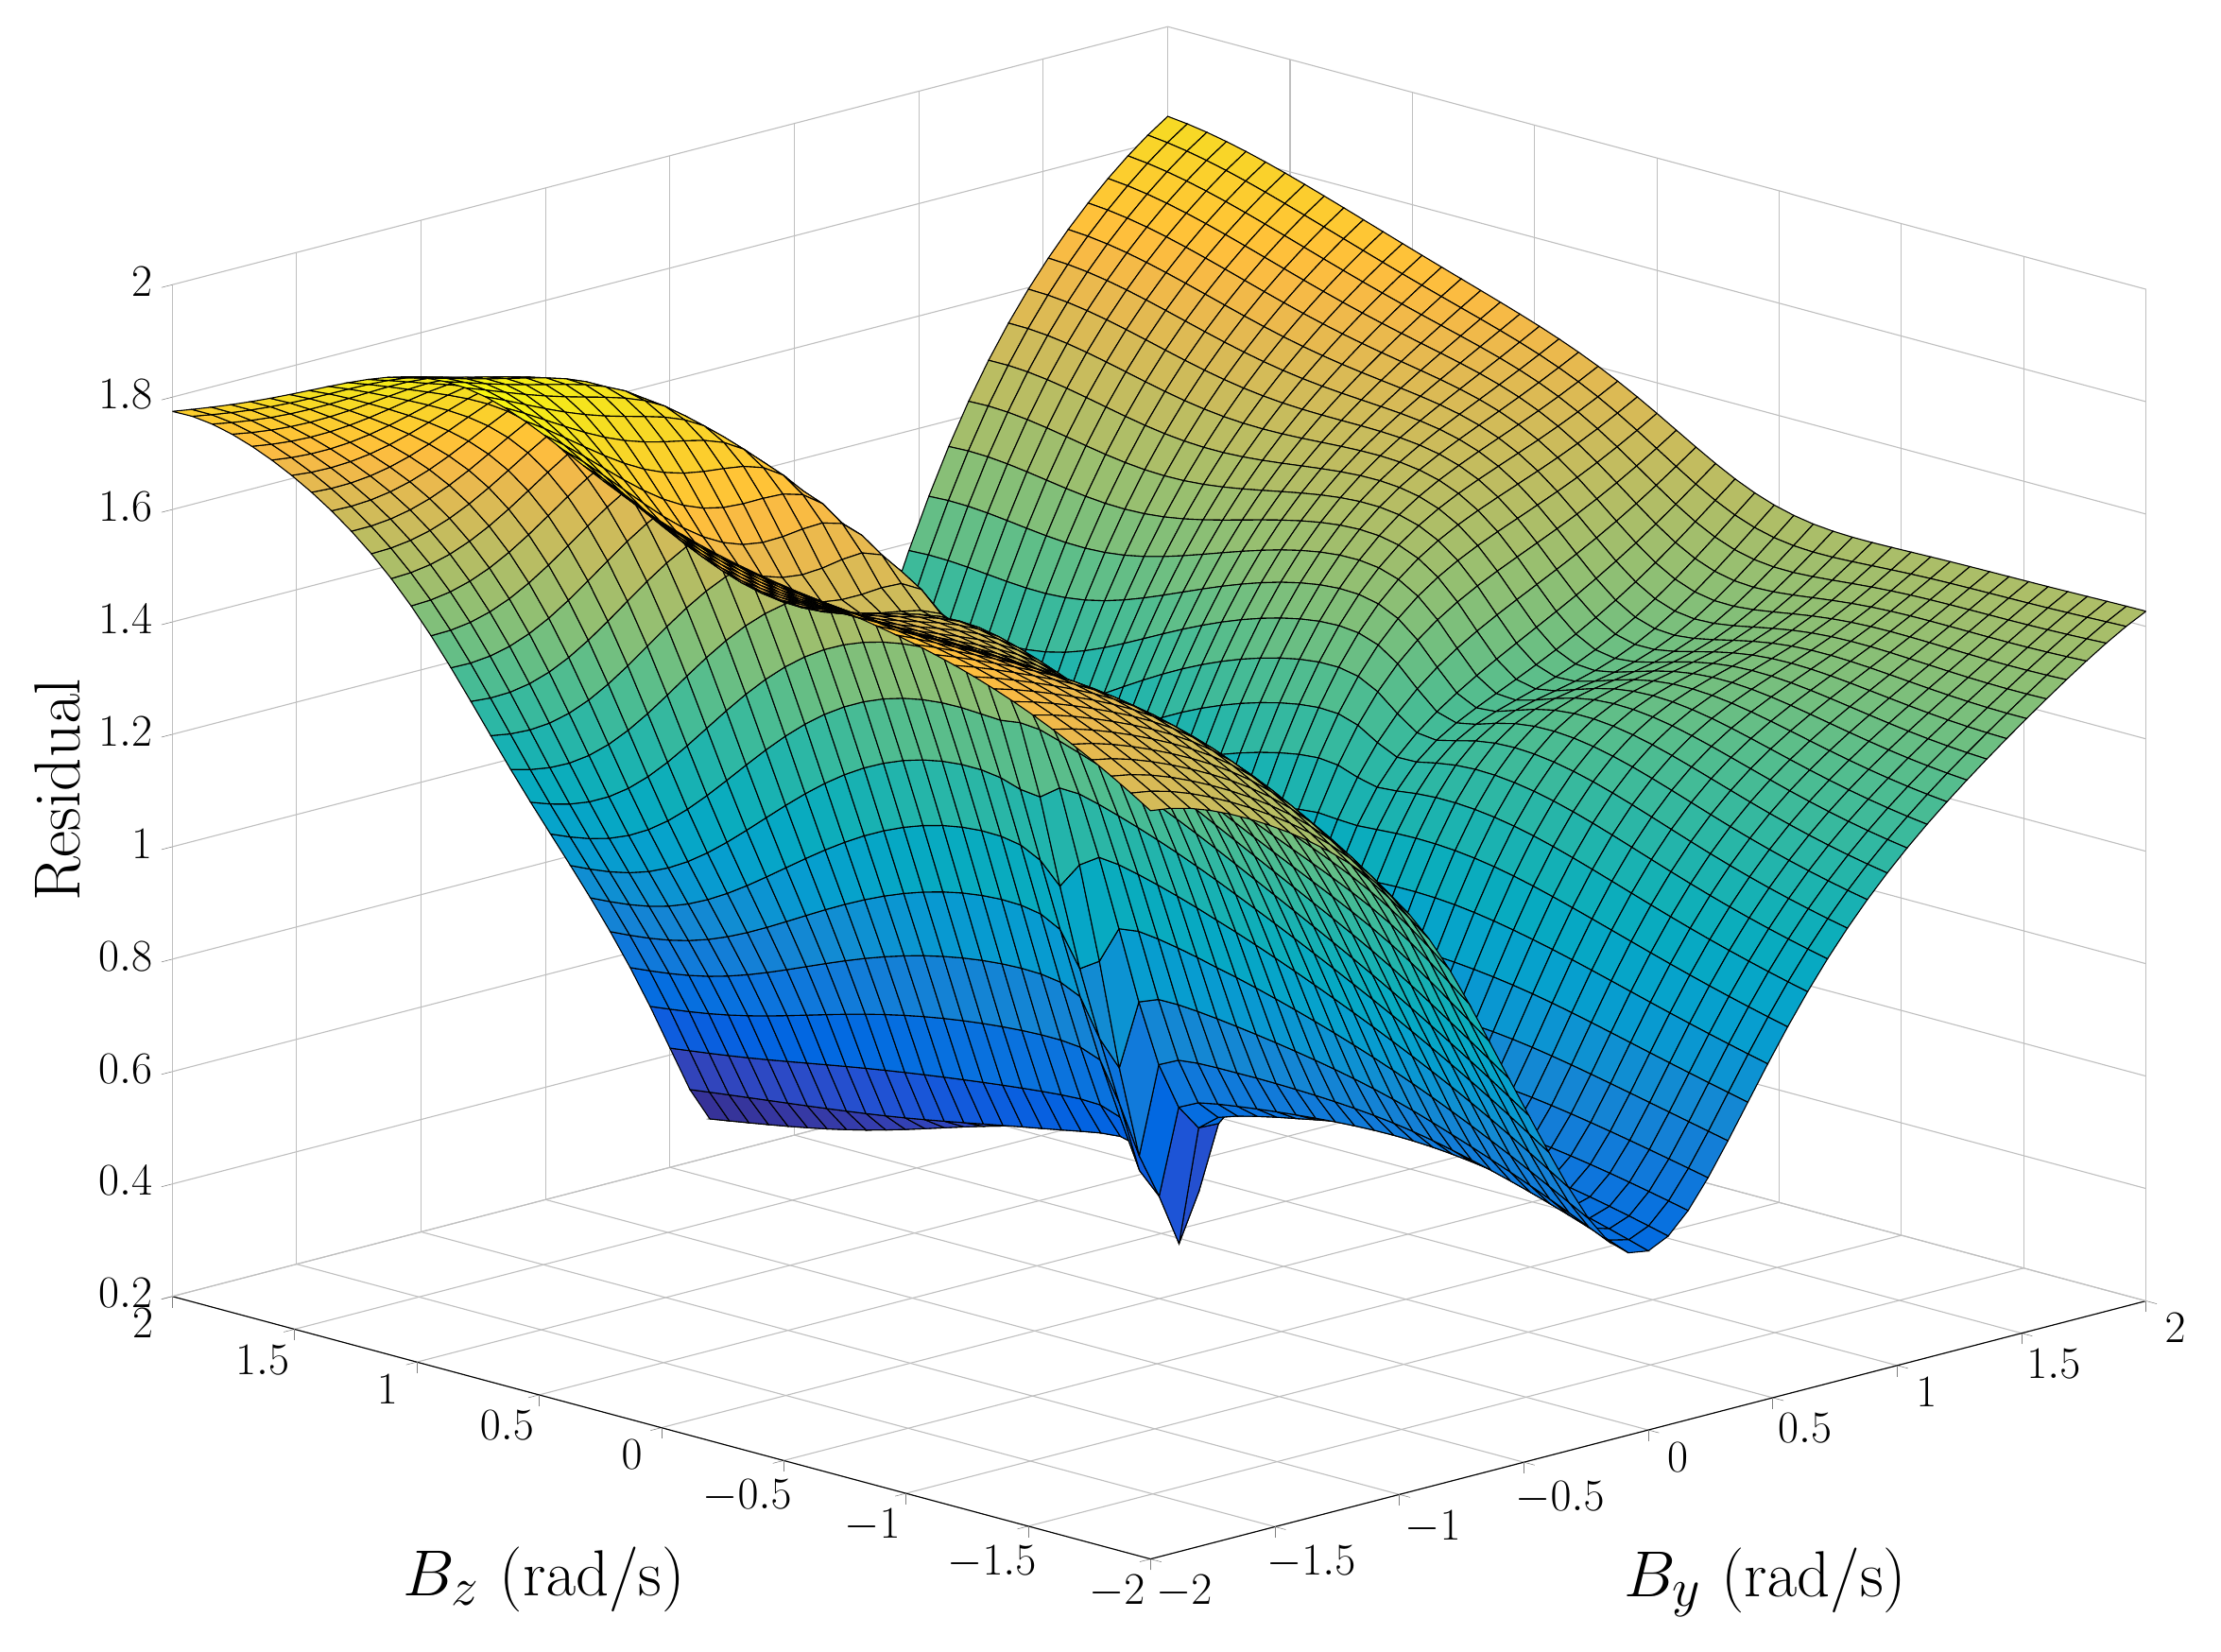
\begin{tikzpicture}

\begin{axis}[%
width=10.442105in,
height=8.107105in,
at={(1.751579in,1.09421in)},
scale only axis,
xmin=-2,
xmax=2,
tick align=outside,
xlabel={\Huge $B_y$ (rad/s)},
xmajorgrids,
ymin=-2,
ymax=2,
ticklabel style = {font=\LARGE},
ylabel={\Huge $B_z$ (rad/s)},
zlabel={\Huge Residual},
ymajorgrids,
zmin=0.2,
zmax=2,
zmajorgrids,
%view={-121.5}{26},
view={-44.5}{20},
axis x line*=bottom,
axis y line*=left,
axis z line*=left
]


\addplot3[%
surf,
faceted color=black,
shader=faceted,
colormap={mymap}{[1pt] rgb(0pt)=(0.2081,0.1663,0.5292); rgb(1pt)=(0.211624,0.189781,0.577676); rgb(2pt)=(0.212252,0.213771,0.626971); rgb(3pt)=(0.2081,0.2386,0.677086); rgb(4pt)=(0.195905,0.264457,0.7279); rgb(5pt)=(0.170729,0.291938,0.779248); rgb(6pt)=(0.125271,0.324243,0.830271); rgb(7pt)=(0.0591333,0.359833,0.868333); rgb(8pt)=(0.0116952,0.38751,0.881957); rgb(9pt)=(0.00595714,0.408614,0.882843); rgb(10pt)=(0.0165143,0.4266,0.878633); rgb(11pt)=(0.0328524,0.443043,0.871957); rgb(12pt)=(0.0498143,0.458571,0.864057); rgb(13pt)=(0.0629333,0.47369,0.855438); rgb(14pt)=(0.0722667,0.488667,0.8467); rgb(15pt)=(0.0779429,0.503986,0.838371); rgb(16pt)=(0.0793476,0.520024,0.831181); rgb(17pt)=(0.0749429,0.537543,0.826271); rgb(18pt)=(0.0640571,0.556986,0.823957); rgb(19pt)=(0.0487714,0.577224,0.822829); rgb(20pt)=(0.0343429,0.596581,0.819852); rgb(21pt)=(0.0265,0.6137,0.8135); rgb(22pt)=(0.0238905,0.628662,0.803762); rgb(23pt)=(0.0230905,0.641786,0.791267); rgb(24pt)=(0.0227714,0.653486,0.776757); rgb(25pt)=(0.0266619,0.664195,0.760719); rgb(26pt)=(0.0383714,0.674271,0.743552); rgb(27pt)=(0.0589714,0.683757,0.725386); rgb(28pt)=(0.0843,0.692833,0.706167); rgb(29pt)=(0.113295,0.7015,0.685857); rgb(30pt)=(0.145271,0.709757,0.664629); rgb(31pt)=(0.180133,0.717657,0.642433); rgb(32pt)=(0.217829,0.725043,0.619262); rgb(33pt)=(0.258643,0.731714,0.595429); rgb(34pt)=(0.302171,0.737605,0.571186); rgb(35pt)=(0.348167,0.742433,0.547267); rgb(36pt)=(0.395257,0.7459,0.524443); rgb(37pt)=(0.44201,0.748081,0.503314); rgb(38pt)=(0.487124,0.749062,0.483976); rgb(39pt)=(0.530029,0.749114,0.466114); rgb(40pt)=(0.570857,0.748519,0.44939); rgb(41pt)=(0.609852,0.747314,0.433686); rgb(42pt)=(0.6473,0.7456,0.4188); rgb(43pt)=(0.683419,0.743476,0.404433); rgb(44pt)=(0.71841,0.741133,0.390476); rgb(45pt)=(0.752486,0.7384,0.376814); rgb(46pt)=(0.785843,0.735567,0.363271); rgb(47pt)=(0.818505,0.732733,0.34979); rgb(48pt)=(0.850657,0.7299,0.336029); rgb(49pt)=(0.882433,0.727433,0.3217); rgb(50pt)=(0.913933,0.725786,0.306276); rgb(51pt)=(0.944957,0.726114,0.288643); rgb(52pt)=(0.973895,0.731395,0.266648); rgb(53pt)=(0.993771,0.745457,0.240348); rgb(54pt)=(0.999043,0.765314,0.216414); rgb(55pt)=(0.995533,0.786057,0.196652); rgb(56pt)=(0.988,0.8066,0.179367); rgb(57pt)=(0.978857,0.827143,0.163314); rgb(58pt)=(0.9697,0.848138,0.147452); rgb(59pt)=(0.962586,0.870514,0.1309); rgb(60pt)=(0.958871,0.8949,0.113243); rgb(61pt)=(0.959824,0.921833,0.0948381); rgb(62pt)=(0.9661,0.951443,0.0755333); rgb(63pt)=(0.9763,0.9831,0.0538)},
mesh/rows=51]
table[row sep=crcr,header=false] {%
%
-2	-2	1.53145545517768\\
-2	-1.92	1.55339432113182\\
-2	-1.84	1.57419507329692\\
-2	-1.76	1.59382356113513\\
-2	-1.68	1.61224504207207\\
-2	-1.6	1.62942849978079\\
-2	-1.52	1.64535085545782\\
-2	-1.44	1.66000053646187\\
-2	-1.36	1.67338021941317\\
-2	-1.28	1.68550887530433\\
-2	-1.2	1.6964234743961\\
-2	-1.12	1.70618082520133\\
-2	-1.04	1.71485997984707\\
-2	-0.96	1.72256538773249\\
-2	-0.88	1.729430503137\\
-2	-0.8	1.73562092812379\\
-2	-0.72	1.7413356253212\\
-2	-0.64	1.74680460952283\\
-2	-0.56	1.75228211376834\\
-2	-0.48	1.75803550296994\\
-2	-0.4	1.76433169113081\\
-2	-0.32	1.77142372566765\\
-2	-0.24	1.77953990238915\\
-2	-0.16	1.78887617495039\\
-2	-0.0800000000000001	1.79959020874615\\
-2	0	1.81179302903385\\
-2	0.0800000000000001	1.82553282079448\\
-2	0.16	1.84076621570844\\
-2	0.24	1.8573165018041\\
-2	0.32	1.87482590453481\\
-2	0.4	1.89271846265956\\
-2	0.48	1.91019621832269\\
-2	0.56	1.92628847017077\\
-2	0.64	1.93995883325904\\
-2	0.72	1.95025215021917\\
-2	0.8	1.95644405160563\\
-2	0.88	1.95815146050906\\
-2	0.96	1.95537559730779\\
-2	1.04	1.94847251708327\\
-2	1.12	1.93806786957263\\
-2	1.2	1.92494402150744\\
-2	1.28	1.90992752411935\\
-2	1.36	1.89379684533984\\
-2	1.44	1.87721956352144\\
-2	1.52	1.86071901538252\\
-2	1.6	1.84466474320825\\
-2	1.68	1.82927906467604\\
-2	1.76	1.81465263124372\\
-2	1.84	1.80076363871893\\
-2	1.92	1.78749739409734\\
-2	2	1.77466466548659\\
-1.92	-2	1.52644024725937\\
-1.92	-1.92	1.54760618723856\\
-1.92	-1.84	1.56769839159649\\
-1.92	-1.76	1.58666494576969\\
-1.92	-1.68	1.6044504385928\\
-1.92	-1.6	1.62100148026256\\
-1.92	-1.52	1.63627181817782\\
-1.92	-1.44	1.65022667515482\\
-1.92	-1.36	1.66284634116721\\
-1.92	-1.28	1.67412934472979\\
-1.92	-1.2	1.68409567236124\\
-1.92	-1.12	1.69279045502597\\
-1.92	-1.04	1.70028826145012\\
-1.92	-0.96	1.70669762903739\\
-1.92	-0.88	1.71216482212205\\
-1.92	-0.8	1.71687528109705\\
-1.92	-0.72	1.72105117483019\\
-1.92	-0.64	1.72494419287864\\
-1.92	-0.56	1.72882419102352\\
-1.92	-0.48	1.7329660337418\\
-1.92	-0.4	1.73763814003155\\
-1.92	-0.32	1.74309612602674\\
-1.92	-0.24	1.7495833255805\\
-1.92	-0.16	1.75733712031624\\
-1.92	-0.0800000000000001	1.76659639070239\\
-1.92	0	1.77760158450565\\
-1.92	0.0800000000000001	1.7905760124368\\
-1.92	0.16	1.80567739425459\\
-1.92	0.24	1.82291582914128\\
-1.92	0.32	1.84205027563081\\
-1.92	0.4	1.86249642808422\\
-1.92	0.48	1.88329252677158\\
-1.92	0.56	1.90316174772088\\
-1.92	0.64	1.92067664841605\\
-1.92	0.72	1.93448764993662\\
-1.92	0.8	1.94354891902119\\
-1.92	0.88	1.94727735372444\\
-1.92	0.96	1.94560913591287\\
-1.92	1.04	1.93895492949051\\
-1.92	1.12	1.92808211017019\\
-1.92	1.2	1.91396359363722\\
-1.92	1.28	1.89762991466958\\
-1.92	1.36	1.88004984427181\\
-1.92	1.44	1.8620508786869\\
-1.92	1.52	1.84427900022976\\
-1.92	1.6	1.82718970876602\\
-1.92	1.68	1.81105969803089\\
-1.92	1.76	1.79600938945147\\
-1.92	1.84	1.78202907166743\\
-1.92	1.92	1.76900422026553\\
-1.92	2	1.75673791736324\\
-1.84	-2	1.51718862747816\\
-1.84	-1.92	1.53787155603612\\
-1.84	-1.84	1.55756184671597\\
-1.84	-1.76	1.57618297776852\\
-1.84	-1.68	1.59365254559981\\
-1.84	-1.6	1.60988872842139\\
-1.84	-1.52	1.6248161162411\\
-1.84	-1.44	1.63837083619051\\
-1.84	-1.36	1.65050532251439\\
-1.84	-1.28	1.6611932851059\\
-1.84	-1.2	1.67043536757623\\
-1.84	-1.12	1.67826561771019\\
-1.84	-1.04	1.68475823147583\\
-1.84	-0.96	1.69003320947629\\
-1.84	-0.88	1.69425889378859\\
-1.84	-0.8	1.69764928229953\\
-1.84	-0.72	1.70045492571023\\
-1.84	-0.64	1.7029480978781\\
-1.84	-0.56	1.70540522812489\\
-1.84	-0.48	1.70809135011194\\
-1.84	-0.4	1.71125174127501\\
-1.84	-0.32	1.71511474807102\\
-1.84	-0.24	1.71990727488401\\
-1.84	-0.16	1.72588082409942\\
-1.84	-0.0800000000000001	1.73334114177774\\
-1.84	0	1.74266811190893\\
-1.84	0.0800000000000001	1.7543054383483\\
-1.84	0.16	1.76869613893341\\
-1.84	0.24	1.7861485018099\\
-1.84	0.32	1.80664608701672\\
-1.84	0.4	1.82966013514918\\
-1.84	0.48	1.85405620810039\\
-1.84	0.56	1.87817217086833\\
-1.84	0.64	1.90007340352574\\
-1.84	0.72	1.91790559472482\\
-1.84	0.8	1.93022498984961\\
-1.84	0.88	1.93621104728495\\
-1.84	0.96	1.93572707127282\\
-1.84	1.04	1.92924814684515\\
-1.84	1.12	1.91770285940816\\
-1.84	1.2	1.90227965473405\\
-1.84	1.28	1.88424069011144\\
-1.84	1.36	1.86477237970092\\
-1.84	1.44	1.84488625591988\\
-1.84	1.52	1.82536973474236\\
-1.84	1.6	1.80677692940669\\
-1.84	1.68	1.78944588348067\\
-1.84	1.76	1.77352938277051\\
-1.84	1.84	1.75902971707145\\
-1.84	1.92	1.74583148211584\\
-1.84	2	1.73372962331688\\
-1.76	-2	1.50439899070418\\
-1.76	-1.92	1.5249164406528\\
-1.76	-1.84	1.54452864764049\\
-1.76	-1.76	1.5631283226072\\
-1.76	-1.68	1.58060022583523\\
-1.76	-1.6	1.59682826074026\\
-1.76	-1.52	1.61170193465027\\
-1.76	-1.44	1.62512257576212\\
-1.76	-1.36	1.63701005264904\\
-1.76	-1.28	1.64731072483388\\
-1.76	-1.2	1.65600689176867\\
-1.76	-1.12	1.66312710607806\\
-1.76	-1.04	1.66875554303287\\
-1.76	-0.96	1.67303758468261\\
-1.76	-0.88	1.67617849221165\\
-1.76	-0.8	1.67843304107066\\
-1.76	-0.72	1.68008633893758\\
-1.76	-0.64	1.68142906850557\\
-1.76	-0.56	1.68273293024016\\
-1.76	-0.48	1.68423310837058\\
-1.76	-0.4	1.6861239144443\\
-1.76	-0.32	1.68857189055647\\
-1.76	-0.24	1.69174816657611\\
-1.76	-0.16	1.69587857045888\\
-1.76	-0.0800000000000001	1.7013044567564\\
-1.76	0	1.70853726835571\\
-1.76	0.0800000000000001	1.71827486659541\\
-1.76	0.16	1.73133350175526\\
-1.76	0.24	1.74845335437028\\
-1.76	0.32	1.76998178230624\\
-1.76	0.4	1.79552907793241\\
-1.76	0.48	1.82377155970885\\
-1.76	0.56	1.85255411355562\\
-1.76	0.64	1.87929449319352\\
-1.76	0.72	1.90152367623051\\
-1.76	0.8	1.91734802922003\\
-1.76	0.88	1.92570419899871\\
-1.76	0.96	1.92639738028795\\
-1.76	1.04	1.91998294947123\\
-1.76	1.12	1.90756247319822\\
-1.76	1.2	1.89055077689722\\
-1.76	1.28	1.87045551678585\\
-1.76	1.36	1.84869842266614\\
-1.76	1.44	1.82649425585957\\
-1.76	1.52	1.80478927079589\\
-1.76	1.6	1.78424927690001\\
-1.76	1.68	1.76528142962033\\
-1.76	1.76	1.74807373091961\\
-1.76	1.84	1.73263971379968\\
-1.76	1.92	1.71886039316407\\
-1.76	2	1.70651960595112\\
-1.68	-2	1.48868705810077\\
-1.68	-1.92	1.50934839511618\\
-1.68	-1.84	1.52918727448515\\
-1.68	-1.76	1.54806055679329\\
-1.68	-1.68	1.56581505457056\\
-1.68	-1.6	1.58229498424194\\
-1.68	-1.52	1.59734925224904\\
-1.68	-1.44	1.6108395627055\\
-1.68	-1.36	1.62265047607551\\
-1.68	-1.28	1.63270208235798\\
-1.68	-1.2	1.64096481351976\\
-1.68	-1.12	1.64747426300051\\
-1.68	-1.04	1.65234222727026\\
-1.68	-0.96	1.65575939323592\\
-1.68	-0.88	1.6579859983261\\
-1.68	-0.8	1.65932960077576\\
-1.68	-0.72	1.66011301074153\\
-1.68	-0.64	1.66063889753262\\
-1.68	-0.56	1.6611592333496\\
-1.68	-0.48	1.66185725672848\\
-1.68	-0.4	1.66284789940048\\
-1.68	-0.32	1.66420086916306\\
-1.68	-0.24	1.66598939867358\\
-1.68	-0.16	1.66836611772915\\
-1.68	-0.0800000000000001	1.6716625562492\\
-1.68	0	1.6764953118892\\
-1.68	0.0800000000000001	1.68383516666328\\
-1.68	0.16	1.69495993154671\\
-1.68	0.24	1.71119716987024\\
-1.68	0.32	1.73342703173264\\
-1.68	0.4	1.76148925201042\\
-1.68	0.48	1.79381944478805\\
-1.68	0.56	1.82760710809784\\
-1.68	0.64	1.8594541788289\\
-1.68	0.72	1.88619135641097\\
-1.68	0.8	1.90548360651703\\
-1.68	0.88	1.91608082503966\\
-1.68	0.96	1.91778224895018\\
-1.68	1.04	1.91124710219501\\
-1.68	1.12	1.89774739593096\\
-1.68	1.2	1.87891088368634\\
-1.68	1.28	1.85648052080453\\
-1.68	1.36	1.83211304824898\\
-1.68	1.44	1.80723531988653\\
-1.68	1.52	1.78296582764801\\
-1.68	1.6	1.76009503470798\\
-1.68	1.68	1.739108437858\\
-1.68	1.76	1.72023359791713\\
-1.68	1.84	1.70349522736797\\
-1.68	1.92	1.68876767239543\\
-1.68	2	1.67581923230383\\
-1.6	-2	1.47052166645262\\
-1.6	-1.92	1.49159443968263\\
-1.6	-1.84	1.51191204550056\\
-1.6	-1.76	1.53129214017272\\
-1.6	-1.68	1.54953988459765\\
-1.6	-1.6	1.56645559485521\\
-1.6	-1.52	1.5818434641774\\
-1.6	-1.44	1.59552301210157\\
-1.6	-1.36	1.60734454644318\\
-1.6	-1.28	1.61720865485938\\
-1.6	-1.2	1.62508761391182\\
-1.6	-1.12	1.63104413619526\\
-1.6	-1.04	1.63524119151477\\
-1.6	-0.96	1.63793705596493\\
-1.6	-0.88	1.6394628843246\\
-1.6	-0.8	1.64018512244746\\
-1.6	-0.72	1.64045986527112\\
-1.6	-0.64	1.64058873253206\\
-1.6	-0.56	1.64078532289629\\
-1.6	-0.48	1.64115893754111\\
-1.6	-0.4	1.64172001545343\\
-1.6	-0.32	1.64241114867808\\
-1.6	-0.24	1.6431689336301\\
-1.6	-0.16	1.6440237413229\\
-1.6	-0.0800000000000001	1.64524235070671\\
-1.6	0	1.64750321897354\\
-1.6	0.0800000000000001	1.65205278517727\\
-1.6	0.16	1.66071916734339\\
-1.6	0.24	1.67559850328926\\
-1.6	0.32	1.69830203072189\\
-1.6	0.4	1.72897295674409\\
-1.6	0.48	1.76567292193836\\
-1.6	0.56	1.80468234388614\\
-1.6	0.64	1.84159891142099\\
-1.6	0.72	1.87253555676131\\
-1.6	0.8	1.89483015858292\\
-1.6	0.88	1.90718854119573\\
-1.6	0.96	1.90949926757377\\
-1.6	1.04	1.90255256465618\\
-1.6	1.12	1.88776685834679\\
-1.6	1.2	1.86693710868261\\
-1.6	1.28	1.8419992144718\\
-1.6	1.36	1.81481930207349\\
-1.6	1.44	1.7870292319971\\
-1.6	1.52	1.759925751642\\
-1.6	1.6	1.73443551868177\\
-1.6	1.68	1.71113326436009\\
-1.6	1.76	1.69029296227886\\
-1.6	1.84	1.67195247881379\\
-1.6	1.92	1.65597739947434\\
-1.6	2	1.64211589642745\\
-1.52	-2	1.45018271786931\\
-1.52	-1.92	1.4718645609199\\
-1.52	-1.84	1.49283235645371\\
-1.52	-1.76	1.51286417165717\\
-1.52	-1.68	1.53172271861929\\
-1.52	-1.6	1.54916307328504\\
-1.52	-1.52	1.5649438257295\\
-1.52	-1.44	1.57884393835398\\
-1.52	-1.36	1.59068616454227\\
-1.52	-1.28	1.60036531211366\\
-1.52	-1.2	1.60787633159441\\
-1.52	-1.12	1.61333434883917\\
-1.52	-1.04	1.61697815191996\\
-1.52	-0.96	1.61915164957285\\
-1.52	-0.88	1.62026396724275\\
-1.52	-0.8	1.62073551744752\\
-1.52	-0.72	1.62094136093743\\
-1.52	-0.64	1.62116292517664\\
-1.52	-0.56	1.62155576047102\\
-1.52	-0.48	1.62213717844446\\
-1.52	-0.4	1.62279581786331\\
-1.52	-0.32	1.623326684927\\
-1.52	-0.24	1.62350004227125\\
-1.52	-0.16	1.62317928746998\\
-1.52	-0.0800000000000001	1.62250687141002\\
-1.52	0	1.62216504524557\\
-1.52	0.0800000000000001	1.62366248828635\\
-1.52	0.16	1.62946975405055\\
-1.52	0.24	1.64266839452534\\
-1.52	0.32	1.66582927573812\\
-1.52	0.4	1.69941735094396\\
-1.52	0.48	1.74083519628824\\
-1.52	0.56	1.78507711125395\\
-1.52	0.64	1.8265707147725\\
-1.52	0.72	1.86083311137317\\
-1.52	0.8	1.88513617084851\\
-1.52	0.88	1.89837169215398\\
-1.52	0.96	1.90063949845215\\
-1.52	1.04	1.8928779042171\\
-1.52	1.12	1.87660073588165\\
-1.52	1.2	1.85369132215521\\
-1.52	1.28	1.82620325062695\\
-1.52	1.36	1.79615858078666\\
-1.52	1.44	1.76536749750189\\
-1.52	1.52	1.73530027391646\\
-1.52	1.6	1.70702774209115\\
-1.52	1.68	1.68122565376886\\
-1.52	1.76	1.65822401865829\\
-1.52	1.84	1.63807870593693\\
-1.52	1.92	1.62064652441191\\
-1.52	2	1.60565191857865\\
-1.44	-2	1.42774261934808\\
-1.44	-1.92	1.45014238726787\\
-1.44	-1.84	1.4718323697837\\
-1.44	-1.76	1.49255564578264\\
-1.44	-1.68	1.51203717057616\\
-1.44	-1.6	1.52999106250382\\
-1.44	-1.52	1.54613513424732\\
-1.44	-1.44	1.56021543075048\\
-1.44	-1.36	1.57204017395491\\
-1.44	-1.28	1.58151800638187\\
-1.44	-1.2	1.58869110328561\\
-1.44	-1.12	1.59375166982083\\
-1.44	-1.04	1.59703260413974\\
-1.44	-0.96	1.59897000539361\\
-1.44	-0.88	1.60004411462393\\
-1.44	-0.8	1.60071177552809\\
-1.44	-0.72	1.60134448492136\\
-1.44	-0.64	1.60218200257117\\
-1.44	-0.56	1.60330556566422\\
-1.44	-0.48	1.60463055102658\\
-1.44	-0.4	1.60591799039026\\
-1.44	-0.32	1.60680827279191\\
-1.44	-0.24	1.60688883656691\\
-1.44	-0.16	1.60582057953159\\
-1.44	-0.0800000000000001	1.60356180431307\\
-1.44	0	1.60072753530133\\
-1.44	0.0800000000000001	1.5990586015586\\
-1.44	0.16	1.60176840507466\\
-1.44	0.24	1.61319240087577\\
-1.44	0.32	1.63711716597696\\
-1.44	0.4	1.67422120450406\\
-1.44	0.48	1.72071779695491\\
-1.44	0.56	1.76982432108066\\
-1.44	0.64	1.81476896231809\\
-1.44	0.72	1.85082684808268\\
-1.44	0.8	1.87561731702724\\
-1.44	0.88	1.8884896612837\\
-1.44	0.96	1.88985880509079\\
-1.44	1.04	1.88079701354864\\
-1.44	1.12	1.86283534081365\\
-1.44	1.2	1.83784325157794\\
-1.44	1.28	1.80789387563129\\
-1.44	1.36	1.77508946229429\\
-1.44	1.44	1.7413729928486\\
-1.44	1.52	1.70837074642449\\
-1.44	1.6	1.67729948624511\\
-1.44	1.68	1.64894665796609\\
-1.44	1.76	1.62370968839726\\
-1.44	1.84	1.60166997535911\\
-1.44	1.92	1.58267792867308\\
-1.44	2	1.56643226546036\\
-1.36	-2	1.40306819327677\\
-1.36	-1.92	1.42620102782304\\
-1.36	-1.84	1.44857991827563\\
-1.36	-1.76	1.4699250886418\\
-1.36	-1.68	1.48993745681206\\
-1.36	-1.6	1.50830375491892\\
-1.36	-1.52	1.52471432531627\\
-1.36	-1.44	1.53889684633689\\
-1.36	-1.36	1.55066271805349\\
-1.36	-1.28	1.55995552372625\\
-1.36	-1.2	1.56688615031561\\
-1.36	-1.12	1.571739936996\\
-1.36	-1.04	1.57494859923953\\
-1.36	-0.96	1.57703108378126\\
-1.36	-0.88	1.57851753934985\\
-1.36	-0.8	1.57987424318505\\
-1.36	-0.72	1.58144355194322\\
-1.36	-0.64	1.58340507619392\\
-1.36	-0.56	1.58575710423637\\
-1.36	-0.48	1.58831398025777\\
-1.36	-0.4	1.59071650285104\\
-1.36	-0.32	1.59245840675585\\
-1.36	-0.24	1.59294355048561\\
-1.36	-0.16	1.59160809704317\\
-1.36	-0.0800000000000001	1.58817080635765\\
-1.36	0	1.58309770693841\\
-1.36	0.0800000000000001	1.57831403569707\\
-1.36	0.16	1.57789118600164\\
-1.36	0.24	1.58775955128533\\
-1.36	0.32	1.61318382875069\\
-1.36	0.4	1.65469107769319\\
-1.36	0.48	1.70643302622806\\
-1.36	0.56	1.75937060426053\\
-1.36	0.64	1.80584700077356\\
-1.36	0.72	1.84154527030709\\
-1.36	0.8	1.86492339569585\\
-1.36	0.88	1.87600242080694\\
-1.36	0.96	1.87553854515291\\
-1.36	1.04	1.86467551129927\\
-1.36	1.12	1.84486514174128\\
-1.36	1.2	1.81785679717632\\
-1.36	1.28	1.78564151860212\\
-1.36	1.36	1.75031739325286\\
-1.36	1.44	1.71390228773723\\
-1.36	1.52	1.67814896714809\\
-1.36	1.6	1.64441347352898\\
-1.36	1.68	1.61360160793295\\
-1.36	1.76	1.58618895325657\\
-1.36	1.84	1.56229107959937\\
-1.36	1.92	1.54175595731323\\
-1.36	2	1.52425591817061\\
-1.28	-2	1.37583428946518\\
-1.28	-1.92	1.39963693667841\\
-1.28	-1.84	1.42257897996783\\
-1.28	-1.76	1.44437947387893\\
-1.28	-1.68	1.46474171685923\\
-1.28	-1.6	1.48335191064776\\
-1.28	-1.52	1.49989736351798\\
-1.28	-1.44	1.51410855118511\\
-1.28	-1.36	1.52581843037068\\
-1.28	-1.28	1.53502098356052\\
-1.28	-1.2	1.54190584163831\\
-1.28	-1.12	1.54685176758759\\
-1.28	-1.04	1.55037670098065\\
-1.28	-0.96	1.55305792203559\\
-1.28	-0.88	1.55544445688294\\
-1.28	-0.8	1.55798197762253\\
-1.28	-0.72	1.56096122952743\\
-1.28	-0.64	1.56449058524725\\
-1.28	-0.56	1.56848655167888\\
-1.28	-0.48	1.57267449984787\\
-1.28	-0.4	1.57659487698709\\
-1.28	-0.32	1.57961728299701\\
-1.28	-0.24	1.58097820545696\\
-1.28	-0.16	1.57988417497012\\
-1.28	-0.0800000000000001	1.57576969177645\\
-1.28	0	1.56886375202162\\
-1.28	0.0800000000000001	1.56121056480383\\
-1.28	0.16	1.55787810017489\\
-1.28	0.24	1.56682732967241\\
-1.28	0.32	1.59499622518268\\
-1.28	0.4	1.64191295287661\\
-1.28	0.48	1.69843883601879\\
-1.28	0.56	1.75315786282672\\
-1.28	0.64	1.79843044946445\\
-1.28	0.72	1.83121942580681\\
-1.28	0.8	1.85120832167398\\
-1.28	0.88	1.85912823554069\\
-1.28	0.96	1.85598529767684\\
-1.28	1.04	1.84288666223187\\
-1.28	1.12	1.82110892441834\\
-1.28	1.2	1.79219424013376\\
-1.28	1.28	1.75796875285063\\
-1.28	1.36	1.72045126443156\\
-1.28	1.44	1.68167538067173\\
-1.28	1.52	1.64348329718382\\
-1.28	1.6	1.60735492441295\\
-1.28	1.68	1.57431432774025\\
-1.28	1.76	1.54492207969571\\
-1.28	1.84	1.51933487665557\\
-1.28	1.92	1.49740174539574\\
-1.28	2	1.47876800989769\\
-1.2	-2	1.34553203577457\\
-1.2	-1.92	1.36990620712269\\
-1.2	-1.84	1.39323233822771\\
-1.2	-1.76	1.41525865673938\\
-1.2	-1.68	1.43573191082655\\
-1.2	-1.6	1.45438104506076\\
-1.2	-1.52	1.47092827844331\\
-1.2	-1.44	1.48513423404312\\
-1.2	-1.36	1.49686812501498\\
-1.2	-1.28	1.50617695248031\\
-1.2	-1.2	1.51332068497503\\
-1.2	-1.12	1.51875245005786\\
-1.2	-1.04	1.52304781985844\\
-1.2	-0.96	1.5268081528838\\
-1.2	-0.88	1.53056780986952\\
-1.2	-0.8	1.53472552034277\\
-1.2	-0.72	1.53950559999043\\
-1.2	-0.64	1.54494334836267\\
-1.2	-0.56	1.55088399808079\\
-1.2	-0.48	1.5569851549838\\
-1.2	-0.4	1.56271670019232\\
-1.2	-0.32	1.5673591530746\\
-1.2	-0.24	1.57001499237964\\
-1.2	-0.16	1.56967788036959\\
-1.2	-0.0800000000000001	1.56547300725506\\
-1.2	0	1.55730737179818\\
-1.2	0.0800000000000001	1.54726482787693\\
-1.2	0.16	1.54158460713647\\
-1.2	0.24	1.55079907511085\\
-1.2	0.32	1.58345069487674\\
-1.2	0.4	1.63641715374951\\
-1.2	0.48	1.69598118970044\\
-1.2	0.56	1.74920386930299\\
-1.2	0.64	1.79000375135208\\
-1.2	0.72	1.81739278636413\\
-1.2	0.8	1.83232868643572\\
-1.2	0.88	1.83605109031717\\
-1.2	0.96	1.82962264359707\\
-1.2	1.04	1.81398965116912\\
-1.2	1.12	1.79018165934937\\
-1.2	1.2	1.75948423747036\\
-1.2	1.28	1.72351152115984\\
-1.2	1.36	1.68415276791665\\
-1.2	1.44	1.64340938818931\\
-1.2	1.52	1.60317586312084\\
-1.2	1.6	1.56503415913547\\
-1.2	1.68	1.53011845719567\\
-1.2	1.76	1.49907414018827\\
-1.2	1.84	1.47210083005076\\
-1.2	1.92	1.44904861732939\\
-1.2	2	1.42953294787297\\
-1.12	-2	1.31144465236158\\
-1.12	-1.92	1.33633456173414\\
-1.12	-1.84	1.35988772471727\\
-1.12	-1.76	1.38191193464829\\
-1.12	-1.68	1.40224999502704\\
-1.12	-1.6	1.42073343443624\\
-1.12	-1.52	1.43717259592484\\
-1.12	-1.44	1.4513934239567\\
-1.12	-1.36	1.4633119779139\\
-1.12	-1.28	1.47301528031367\\
-1.12	-1.2	1.48080417707717\\
-1.12	-1.12	1.48716848561668\\
-1.12	-1.04	1.49270178782309\\
-1.12	-0.96	1.4979928669871\\
-1.12	-0.88	1.50353230396689\\
-1.12	-0.8	1.50965384742339\\
-1.12	-0.72	1.51650990210759\\
-1.12	-0.64	1.52406929545738\\
-1.12	-0.56	1.53212329413428\\
-1.12	-0.48	1.54028858059776\\
-1.12	-0.4	1.54800032886875\\
-1.12	-0.32	1.55449429876802\\
-1.12	-0.24	1.55878843886671\\
-1.12	-0.16	1.55970606473224\\
-1.12	-0.0800000000000001	1.55606967130312\\
-1.12	0	1.54739933641697\\
-1.12	0.0800000000000001	1.53573762786159\\
-1.12	0.16	1.52872381132889\\
-1.12	0.24	1.54006717880295\\
-1.12	0.32	1.57913660888112\\
-1.12	0.4	1.63747032009233\\
-1.12	0.48	1.69641753014758\\
-1.12	0.56	1.74392264981585\\
-1.12	0.64	1.77713091681248\\
-1.12	0.72	1.79726270614689\\
-1.12	0.8	1.80613996387441\\
-1.12	0.88	1.80512982884705\\
-1.12	0.96	1.79513035111658\\
-1.12	1.04	1.77683054522337\\
-1.12	1.12	1.75098424578094\\
-1.12	1.2	1.71861639348777\\
-1.12	1.28	1.68112372167301\\
-1.12	1.36	1.64024878018488\\
-1.12	1.44	1.59793363952566\\
-1.12	1.52	1.55609596121313\\
-1.12	1.6	1.51639613366\\
-1.12	1.68	1.48006297963603\\
-1.12	1.76	1.44781745660413\\
-1.12	1.84	1.41989540366324\\
-1.12	1.92	1.39614101144902\\
-1.12	2	1.37613180311409\\
-1.04	-2	1.27256209639071\\
-1.04	-1.92	1.29805748878543\\
-1.04	-1.84	1.32182095238716\\
-1.04	-1.76	1.34372408501184\\
-1.04	-1.68	1.36375508899567\\
-1.04	-1.6	1.38191797649542\\
-1.04	-1.52	1.39817896928891\\
-1.04	-1.44	1.41247697061749\\
-1.04	-1.36	1.42478929633909\\
-1.04	-1.28	1.43522151642482\\
-1.04	-1.2	1.44406939843994\\
-1.04	-1.12	1.45180712821194\\
-1.04	-1.04	1.45900094939117\\
-1.04	-0.96	1.46619382370138\\
-1.04	-0.88	1.47381209484217\\
-1.04	-0.8	1.48211632890105\\
-1.04	-0.72	1.49118993758894\\
-1.04	-0.64	1.50094771059648\\
-1.04	-0.56	1.51114752191849\\
-1.04	-0.48	1.52139354247489\\
-1.04	-0.4	1.53112376449209\\
-1.04	-0.32	1.53957840284612\\
-1.04	-0.24	1.54575356104241\\
-1.04	-0.16	1.5483727993893\\
-1.04	-0.0800000000000001	1.54600783916341\\
-1.04	0	1.53777358731758\\
-1.04	0.0800000000000001	1.5256158601071\\
-1.04	0.16	1.51887615198656\\
-1.04	0.24	1.5349095835334\\
-1.04	0.32	1.58160316596833\\
-1.04	0.4	1.64198103638458\\
-1.04	0.48	1.69482716008452\\
-1.04	0.56	1.73251357415863\\
-1.04	0.64	1.75607009875735\\
-1.04	0.72	1.76817550855278\\
-1.04	0.8	1.77080121256969\\
-1.04	0.88	1.76505256827358\\
-1.04	0.96	1.7515061304398\\
-1.04	1.04	1.73055906219533\\
-1.04	1.12	1.70270957386855\\
-1.04	1.2	1.6687586876903\\
-1.04	1.28	1.62991724252966\\
-1.04	1.36	1.58779644565231\\
-1.04	1.44	1.54427659148842\\
-1.04	1.52	1.50128336191276\\
-1.04	1.6	1.46053495947515\\
-1.04	1.68	1.42333404573465\\
-1.04	1.76	1.39045793644258\\
-1.04	1.84	1.3621606740808\\
-1.04	1.92	1.33826323129929\\
-1.04	2	1.31828898836919\\
-0.96	-2	1.22745404241705\\
-0.96	-1.92	1.25385418198294\\
-0.96	-1.84	1.27809201660122\\
-0.96	-1.76	1.30002204826444\\
-0.96	-1.68	1.31978098432526\\
-0.96	-1.6	1.33760351778539\\
-0.96	-1.52	1.35368599006551\\
-0.96	-1.44	1.36814378985868\\
-0.96	-1.36	1.38104912171719\\
-0.96	-1.28	1.39251731958251\\
-0.96	-1.2	1.40279294687586\\
-0.96	-1.12	1.41227514073736\\
-0.96	-1.04	1.42145447157208\\
-0.96	-0.96	1.43079979205861\\
-0.96	-0.88	1.4406619369556\\
-0.96	-0.8	1.45122881930677\\
-0.96	-0.72	1.46252368936852\\
-0.96	-0.64	1.47442236428898\\
-0.96	-0.56	1.48666965990084\\
-0.96	-0.48	1.4988833972233\\
-0.96	-0.4	1.51053911469669\\
-0.96	-0.32	1.52093020347407\\
-0.96	-0.24	1.52910120533242\\
-0.96	-0.16	1.53377261215813\\
-0.96	-0.0800000000000001	1.53337401200442\\
-0.96	0	1.52667904268168\\
-0.96	0.0800000000000001	1.5155543985778\\
-0.96	0.16	1.5114125825266\\
-0.96	0.24	1.53496709165036\\
-0.96	0.32	1.58785164001635\\
-0.96	0.4	1.64359101436594\\
-0.96	0.48	1.68460016292437\\
-0.96	0.56	1.71004351645376\\
-0.96	0.64	1.72359916720809\\
-0.96	0.72	1.72808748528329\\
-0.96	0.8	1.72498153089744\\
-0.96	0.88	1.71489848349202\\
-0.96	0.96	1.69805357127287\\
-0.96	1.04	1.67458540805737\\
-0.96	1.12	1.64479607083419\\
-0.96	1.2	1.60932729135168\\
-0.96	1.28	1.56926116046117\\
-0.96	1.36	1.52611839922319\\
-0.96	1.44	1.48173767476295\\
-0.96	1.52	1.43805287178607\\
-0.96	1.6	1.39682477378206\\
-0.96	1.68	1.35940485557128\\
-0.96	1.76	1.32659666705116\\
-0.96	1.84	1.29864071690438\\
-0.96	1.92	1.27530430747951\\
-0.96	2	1.25603011406877\\
-0.88	-2	1.17432330457918\\
-0.88	-1.92	1.20196671383972\\
-0.88	-1.84	1.22725311001733\\
-0.88	-1.76	1.24978525394877\\
-0.88	-1.68	1.26970442968577\\
-0.88	-1.6	1.28745703621822\\
-0.88	-1.52	1.30352135662854\\
-0.88	-1.44	1.31826011382113\\
-0.88	-1.36	1.33190288489411\\
-0.88	-1.28	1.34460746436943\\
-0.88	-1.2	1.35655438886828\\
-0.88	-1.12	1.36802005685374\\
-0.88	-1.04	1.37937033733759\\
-0.88	-0.96	1.39097295332421\\
-0.88	-0.88	1.40309767811498\\
-0.88	-0.8	1.41586609525001\\
-0.88	-0.72	1.42925311964669\\
-0.88	-0.64	1.44311045540176\\
-0.88	-0.56	1.45718722236407\\
-0.88	-0.48	1.47113580692907\\
-0.88	-0.4	1.48449720167066\\
-0.88	-0.32	1.49666011612534\\
-0.88	-0.24	1.50678661914669\\
-0.88	-0.16	1.51370775473655\\
-0.88	-0.0800000000000001	1.51587841432184\\
-0.88	0	1.51191350964031\\
-0.88	0.0800000000000001	1.50375583233721\\
-0.88	0.16	1.50518495553518\\
-0.88	0.24	1.53779044221022\\
-0.88	0.32	1.59048195627245\\
-0.88	0.4	1.63335123278368\\
-0.88	0.48	1.65932532408454\\
-0.88	0.56	1.6728072235829\\
-0.88	0.64	1.67766596430908\\
-0.88	0.72	1.67580019975762\\
-0.88	0.8	1.66790692456981\\
-0.88	0.88	1.65410892741704\\
-0.88	0.96	1.63432673315678\\
-0.88	1.04	1.60852107159383\\
-0.88	1.12	1.5768788915103\\
-0.88	1.2	1.53996049841843\\
-0.88	1.28	1.4987897222898\\
-0.88	1.36	1.45485325367992\\
-0.88	1.44	1.40998377229887\\
-0.88	1.52	1.36613437867351\\
-0.88	1.6	1.32509560390559\\
-0.88	1.68	1.28823589246614\\
-0.88	1.76	1.25634134344976\\
-0.88	1.84	1.22959119721753\\
-0.88	1.92	1.20765437942129\\
-0.88	2	1.18985646476419\\
-0.8	-2	1.11183405749684\\
-0.8	-1.92	1.14046131370121\\
-0.8	-1.84	1.16722645261127\\
-0.8	-1.76	1.19124515773911\\
-0.8	-1.68	1.21227992902931\\
-0.8	-1.6	1.23073330925837\\
-0.8	-1.52	1.24729412668447\\
-0.8	-1.44	1.26260559739698\\
-0.8	-1.36	1.27712647189667\\
-0.8	-1.28	1.29113727234788\\
-0.8	-1.2	1.30481235926491\\
-0.8	-1.12	1.31831231605159\\
-0.8	-1.04	1.33184632422591\\
-0.8	-0.96	1.34565147713289\\
-0.8	-0.88	1.35990931917342\\
-0.8	-0.8	1.37468260407177\\
-0.8	-0.72	1.38990991642784\\
-0.8	-0.64	1.40543154431205\\
-0.8	-0.56	1.42101376123753\\
-0.8	-0.48	1.43635744878255\\
-0.8	-0.4	1.45108714542051\\
-0.8	-0.32	1.46471644402754\\
-0.8	-0.24	1.4765813379805\\
-0.8	-0.16	1.48573550591952\\
-0.8	-0.0800000000000001	1.49086797097527\\
-0.8	0	1.49075186464216\\
-0.8	0.0800000000000001	1.48774025229502\\
-0.8	0.16	1.49762147553193\\
-0.8	0.24	1.53618175091432\\
-0.8	0.32	1.57783251968747\\
-0.8	0.4	1.602948338631\\
-0.8	0.48	1.61505420255714\\
-0.8	0.56	1.61916531457801\\
-0.8	0.64	1.61754827455358\\
-0.8	0.72	1.61090709543632\\
-0.8	0.8	1.59927008030227\\
-0.8	0.88	1.58241225948957\\
-0.8	0.96	1.56008086091536\\
-0.8	1.04	1.53215666072531\\
-0.8	1.12	1.49879696735287\\
-0.8	1.2	1.46056040405018\\
-0.8	1.28	1.41848618084808\\
-0.8	1.36	1.37408800888665\\
-0.8	1.44	1.3292317559606\\
-0.8	1.52	1.28589958435664\\
-0.8	1.6	1.24589056789839\\
-0.8	1.68	1.21054320287389\\
-0.8	1.76	1.18056429247222\\
-0.8	1.84	1.15600781776057\\
-0.8	1.92	1.13638928487037\\
-0.8	2	1.12087793167302\\
-0.72	-2	1.04095642387479\\
-0.72	-1.92	1.06916007003082\\
-0.72	-1.84	1.09661097042786\\
-0.72	-1.76	1.12230613063954\\
-0.72	-1.68	1.14541919961879\\
-0.72	-1.6	1.16577794300599\\
-0.72	-1.52	1.18386784384054\\
-0.72	-1.44	1.20044677321872\\
-0.72	-1.36	1.21619645642883\\
-0.72	-1.28	1.23158991331345\\
-0.72	-1.2	1.24690303807664\\
-0.72	-1.12	1.26227972805565\\
-0.72	-1.04	1.27781240889992\\
-0.72	-0.96	1.29359698920037\\
-0.72	-0.88	1.30971387172583\\
-0.72	-0.8	1.32616915291231\\
-0.72	-0.72	1.34287396000493\\
-0.72	-0.64	1.35966645101332\\
-0.72	-0.56	1.37633814552787\\
-0.72	-0.48	1.39264521047208\\
-0.72	-0.4	1.40830273093365\\
-0.72	-0.32	1.42296159406039\\
-0.72	-0.24	1.43616318944426\\
-0.72	-0.16	1.44726701976877\\
-0.72	-0.0800000000000001	1.4553986568028\\
-0.72	0	1.459890925769\\
-0.72	0.0800000000000001	1.46389637395027\\
-0.72	0.16	1.48261848371128\\
-0.72	0.24	1.51657082546971\\
-0.72	0.32	1.53900649821597\\
-0.72	0.4	1.54858902243018\\
-0.72	0.48	1.55125196965844\\
-0.72	0.56	1.54939280052875\\
-0.72	0.64	1.54353816275389\\
-0.72	0.72	1.53355575263411\\
-0.72	0.8	1.5190959475916\\
-0.72	0.88	1.49977450066243\\
-0.72	0.96	1.4752898545744\\
-0.72	1.04	1.44553557917654\\
-0.72	1.12	1.4107192179073\\
-0.72	1.2	1.37147220638057\\
-0.72	1.28	1.32891623633305\\
-0.72	1.36	1.28464273630015\\
-0.72	1.44	1.24057351804455\\
-0.72	1.52	1.19870661281247\\
-0.72	1.6	1.1608011534978\\
-0.72	1.68	1.12809254538266\\
-0.72	1.76	1.10112764152411\\
-0.72	1.84	1.07976436233796\\
-0.72	1.92	1.06331571130179\\
-0.72	2	1.05077110221777\\
-0.64	-2	0.965623565518185\\
-0.64	-1.92	0.991947477269978\\
-0.64	-1.84	1.01814454181198\\
-0.64	-1.76	1.04383334171551\\
-0.64	-1.68	1.06832820135391\\
-0.64	-1.6	1.09095493546456\\
-0.64	-1.52	1.11149657528623\\
-0.64	-1.44	1.1302902775276\\
-0.64	-1.36	1.14794474896629\\
-0.64	-1.28	1.16503420970769\\
-0.64	-1.2	1.18196383839193\\
-0.64	-1.12	1.19896447421338\\
-0.64	-1.04	1.21613627606765\\
-0.64	-0.96	1.23350597954463\\
-0.64	-0.88	1.25106598481578\\
-0.64	-0.8	1.26876371682348\\
-0.64	-0.72	1.28648415230663\\
-0.64	-0.64	1.30406726717592\\
-0.64	-0.56	1.32133368967426\\
-0.64	-0.48	1.33809604340539\\
-0.64	-0.4	1.35415697310065\\
-0.64	-0.32	1.36929842608312\\
-0.64	-0.24	1.38326426285754\\
-0.64	-0.16	1.39574262010627\\
-0.64	-0.0800000000000001	1.40640688028174\\
-0.64	0	1.41544220407276\\
-0.64	0.0800000000000001	1.42659432101047\\
-0.64	0.16	1.44766052792555\\
-0.64	0.24	1.46476952911964\\
-0.64	0.32	1.47082399896417\\
-0.64	0.4	1.47186889285325\\
-0.64	0.48	1.46986177832652\\
-0.64	0.56	1.46484958399936\\
-0.64	0.64	1.4564553807904\\
-0.64	0.72	1.44421731199899\\
-0.64	0.8	1.42768054776549\\
-0.64	0.88	1.40645659617615\\
-0.64	0.96	1.38029645469766\\
-0.64	1.04	1.34918545663999\\
-0.64	1.12	1.3134507670691\\
-0.64	1.2	1.27385696546673\\
-0.64	1.28	1.23165131896279\\
-0.64	1.36	1.1885164557043\\
-0.64	1.44	1.14640414968924\\
-0.64	1.52	1.10726255715492\\
-0.64	1.6	1.07271798816091\\
-0.64	1.68	1.04380504750761\\
-0.64	1.76	1.02083142127566\\
-0.64	1.84	1.00341350598771\\
-0.64	1.92	0.990653024701587\\
-0.64	2	0.981380097595388\\
-0.56	-2	0.889787916597337\\
-0.56	-1.92	0.914370012664734\\
-0.56	-1.84	0.938609147503905\\
-0.56	-1.76	0.962579085388017\\
-0.56	-1.68	0.986224928425647\\
-0.56	-1.6	1.00924944005078\\
-0.56	-1.52	1.03124918088641\\
-0.56	-1.44	1.05201686248061\\
-0.56	-1.36	1.07168211667762\\
-0.56	-1.28	1.0905864888147\\
-0.56	-1.2	1.10908718028801\\
-0.56	-1.12	1.1274458809597\\
-0.56	-1.04	1.14580692179985\\
-0.56	-0.96	1.16421917157336\\
-0.56	-0.88	1.18266320763605\\
-0.56	-0.8	1.20105153040115\\
-0.56	-0.72	1.21923602136008\\
-0.56	-0.64	1.23705313423769\\
-0.56	-0.56	1.25435228612028\\
-0.56	-0.48	1.27100032751183\\
-0.56	-0.4	1.28687795219364\\
-0.56	-0.32	1.30187625759861\\
-0.56	-0.24	1.31590176239664\\
-0.56	-0.16	1.32890757862755\\
-0.56	-0.0800000000000001	1.34101793100414\\
-0.56	0	1.35299791326847\\
-0.56	0.0800000000000001	1.36666479822976\\
-0.56	0.16	1.37646286816258\\
-0.56	0.24	1.37826239155265\\
-0.56	0.32	1.37843882208997\\
-0.56	0.4	1.37717038622045\\
-0.56	0.48	1.37362288463349\\
-0.56	0.56	1.36717609899707\\
-0.56	0.64	1.35732789804232\\
-0.56	0.72	1.34363276186001\\
-0.56	0.8	1.32570264215557\\
-0.56	0.88	1.30324771060197\\
-0.56	0.96	1.27614688740148\\
-0.56	1.04	1.24453892406588\\
-0.56	1.12	1.20891729142471\\
-0.56	1.2	1.17020098078512\\
-0.56	1.28	1.12974509792575\\
-0.56	1.36	1.08925818789975\\
-0.56	1.44	1.0506138531989\\
-0.56	1.52	1.01558058348047\\
-0.56	1.6	0.985532601187067\\
-0.56	1.68	0.961225373788506\\
-0.56	1.76	0.942705800349739\\
-0.56	1.84	0.929380053535183\\
-0.56	1.92	0.92020457367846\\
-0.56	2	0.913928722396219\\
-0.48	-2	0.814670568287115\\
-0.48	-1.92	0.83851140356358\\
-0.48	-1.84	0.861739897103438\\
-0.48	-1.76	0.884375931811501\\
-0.48	-1.68	0.906543117649048\\
-0.48	-1.6	0.928339400631662\\
-0.48	-1.52	0.949724053002236\\
-0.48	-1.44	0.970553219651552\\
-0.48	-1.36	0.990732689188013\\
-0.48	-1.28	1.01031005687462\\
-0.48	-1.2	1.02943375582876\\
-0.48	-1.12	1.04826276088968\\
-0.48	-1.04	1.06690709464771\\
-0.48	-0.96	1.08541539724256\\
-0.48	-0.88	1.10381311578814\\
-0.48	-0.8	1.12212168013929\\
-0.48	-0.72	1.14012880718939\\
-0.48	-0.64	1.15754549083373\\
-0.48	-0.56	1.17425160905144\\
-0.48	-0.48	1.1901654402904\\
-0.48	-0.4	1.20523029001342\\
-0.48	-0.32	1.21941545508409\\
-0.48	-0.24	1.23272101250509\\
-0.48	-0.16	1.24520610595672\\
-0.48	-0.0800000000000001	1.25701076492958\\
-0.48	0	1.2677527008836\\
-0.48	0.0800000000000001	1.27067008773957\\
-0.48	0.16	1.26561262231659\\
-0.48	0.24	1.26764766774829\\
-0.48	0.32	1.2694832062804\\
-0.48	0.4	1.26874767170341\\
-0.48	0.48	1.26500452754484\\
-0.48	0.56	1.25798895512723\\
-0.48	0.64	1.24742162307924\\
-0.48	0.72	1.23302098276702\\
-0.48	0.8	1.21454957677569\\
-0.48	0.88	1.19187703981373\\
-0.48	0.96	1.16505585613232\\
-0.48	1.04	1.13440125331366\\
-0.48	1.12	1.10055863852384\\
-0.48	1.2	1.06453541294856\\
-0.48	1.28	1.02767316550586\\
-0.48	1.36	0.991544515326656\\
-0.48	1.44	0.957776536222199\\
-0.48	1.52	0.927826043834863\\
-0.48	1.6	0.9027540344914\\
-0.48	1.68	0.883057998215358\\
-0.48	1.76	0.868612458556087\\
-0.48	1.84	0.858737019050904\\
-0.48	1.92	0.85236829389347\\
-0.48	2	0.848279208460639\\
-0.4	-2	0.740190018739785\\
-0.4	-1.92	0.763518723852007\\
-0.4	-1.84	0.786326625317818\\
-0.4	-1.76	0.80843883377133\\
-0.4	-1.68	0.829798869596202\\
-0.4	-1.6	0.850470213092075\\
-0.4	-1.52	0.870569537256024\\
-0.4	-1.44	0.890180956457625\\
-0.4	-1.36	0.909332990614989\\
-0.4	-1.28	0.928042301351578\\
-0.4	-1.2	0.946348945974496\\
-0.4	-1.12	0.964307459793696\\
-0.4	-1.04	0.981961089334561\\
-0.4	-0.96	0.999322429516027\\
-0.4	-0.88	1.01635801447313\\
-0.4	-0.8	1.03298692111795\\
-0.4	-0.72	1.0493381651035\\
-0.4	-0.64	1.06557678948035\\
-0.4	-0.56	1.08092194775366\\
-0.4	-0.48	1.0954206723698\\
-0.4	-0.4	1.10901204549515\\
-0.4	-0.32	1.12169495408537\\
-0.4	-0.24	1.13348223946535\\
-0.4	-0.16	1.14430250171199\\
-0.4	-0.0800000000000001	1.1534274218753\\
-0.4	0	1.15460528338151\\
-0.4	0.0800000000000001	1.12934160658966\\
-0.4	0.16	1.1333506664844\\
-0.4	0.24	1.14473195986991\\
-0.4	0.32	1.14955536545133\\
-0.4	0.4	1.14972727082958\\
-0.4	0.48	1.14617216587349\\
-0.4	0.56	1.13913591363704\\
-0.4	0.64	1.12860483808095\\
-0.4	0.72	1.11448984219378\\
-0.4	0.8	1.09672850141415\\
-0.4	0.88	1.07536101776639\\
-0.4	0.96	1.05059480716514\\
-0.4	1.04	1.0228563729693\\
-0.4	1.12	0.992822365700295\\
-0.4	1.2	0.961419981591805\\
-0.4	1.28	0.929788526374023\\
-0.4	1.36	0.899197864465732\\
-0.4	1.44	0.870925138586055\\
-0.4	1.52	0.846099680349369\\
-0.4	1.6	0.825538766065286\\
-0.4	1.68	0.809611155789003\\
-0.4	1.76	0.798171548974913\\
-0.4	1.84	0.790595730759734\\
-0.4	1.92	0.785912846202725\\
-0.4	2	0.782994884337931\\
-0.32	-2	0.668161374961298\\
-0.32	-1.92	0.690045311784276\\
-0.32	-1.84	0.711652052993323\\
-0.32	-1.76	0.732776775447529\\
-0.32	-1.68	0.75324266332012\\
-0.32	-1.6	0.772935588665817\\
-0.32	-1.52	0.791825751146868\\
-0.32	-1.44	0.809961877728524\\
-0.32	-1.36	0.82743854113291\\
-0.32	-1.28	0.844355040576789\\
-0.32	-1.2	0.860787944473305\\
-0.32	-1.12	0.876783362430601\\
-0.32	-1.04	0.892361059628844\\
-0.32	-0.96	0.907522809792173\\
-0.32	-0.88	0.922259884280343\\
-0.32	-0.8	0.936552391768544\\
-0.32	-0.72	0.950353669979925\\
-0.32	-0.64	0.963565784463703\\
-0.32	-0.56	0.975887141060775\\
-0.32	-0.48	0.988292124950305\\
-0.32	-0.4	0.999763910870124\\
-0.32	-0.32	1.01024329110829\\
-0.32	-0.24	1.01972372573134\\
-0.32	-0.16	1.02774304424313\\
-0.32	-0.0800000000000001	1.03133485496807\\
-0.32	0	1.00850615990833\\
-0.32	0.0800000000000001	0.961381328369265\\
-0.32	0.16	0.998107740021605\\
-0.32	0.24	1.01582562854028\\
-0.32	0.32	1.02209102073056\\
-0.32	0.4	1.02277841031193\\
-0.32	0.48	1.0196445836542\\
-0.32	0.56	1.01324972979355\\
-0.32	0.64	1.00377045793546\\
-0.32	0.72	0.991270052276135\\
-0.32	0.8	0.975815581310534\\
-0.32	0.88	0.957542843691323\\
-0.32	0.96	0.936698476752249\\
-0.32	1.04	0.913667943754513\\
-0.32	1.12	0.888991265351924\\
-0.32	1.2	0.863365206921391\\
-0.32	1.28	0.837627993937318\\
-0.32	1.36	0.812720042809474\\
-0.32	1.44	0.789613288656006\\
-0.32	1.52	0.769205762569226\\
-0.32	1.6	0.752190133338956\\
-0.32	1.68	0.738923494047961\\
-0.32	1.76	0.729340962618388\\
-0.32	1.84	0.7229528974069\\
-0.32	1.92	0.718938057656752\\
-0.32	2	0.716305693235713\\
-0.24	-2	0.60374163253934\\
-0.24	-1.92	0.62300996226216\\
-0.24	-1.84	0.642033867650268\\
-0.24	-1.76	0.66066894998138\\
-0.24	-1.68	0.678788974508853\\
-0.24	-1.6	0.6963073625951\\
-0.24	-1.52	0.713194156395045\\
-0.24	-1.44	0.729467196906061\\
-0.24	-1.36	0.745135680692525\\
-0.24	-1.28	0.760134436058642\\
-0.24	-1.2	0.774363455937756\\
-0.24	-1.12	0.787801039587018\\
-0.24	-1.04	0.800514064394184\\
-0.24	-0.96	0.812586389881649\\
-0.24	-0.88	0.824076720750075\\
-0.24	-0.8	0.835017167431824\\
-0.24	-0.72	0.845423749465615\\
-0.24	-0.64	0.855296059610816\\
-0.24	-0.56	0.864563287328389\\
-0.24	-0.48	0.872688971830618\\
-0.24	-0.4	0.88156753159748\\
-0.24	-0.32	0.889262886372731\\
-0.24	-0.24	0.895651252642147\\
-0.24	-0.16	0.899855619337017\\
-0.24	-0.0800000000000001	0.895093045811452\\
-0.24	0	0.827934813306171\\
-0.24	0.0800000000000001	0.805382104575967\\
-0.24	0.16	0.865601210333892\\
-0.24	0.24	0.884103166363298\\
-0.24	0.32	0.890307781625491\\
-0.24	0.4	0.891273049149369\\
-0.24	0.48	0.888938635049488\\
-0.24	0.56	0.883958222026553\\
-0.24	0.64	0.876581443073629\\
-0.24	0.72	0.866923175637515\\
-0.24	0.8	0.855068598138227\\
-0.24	0.88	0.841125266315721\\
-0.24	0.96	0.825256031222318\\
-0.24	1.04	0.807704218337532\\
-0.24	1.12	0.78881413744722\\
-0.24	1.2	0.769045583179956\\
-0.24	1.28	0.748977605029086\\
-0.24	1.36	0.729293891203972\\
-0.24	1.44	0.710740603957832\\
-0.24	1.52	0.694049952175997\\
-0.24	1.6	0.67983224444221\\
-0.24	1.68	0.668455935385214\\
-0.24	1.76	0.659952469985876\\
-0.24	1.84	0.653986898678965\\
-0.24	1.92	0.649915936703967\\
-0.24	2	0.646918865910609\\
-0.16	-2	0.553825934156165\\
-0.16	-1.92	0.569986690258262\\
-0.16	-1.84	0.585809803408516\\
-0.16	-1.76	0.601175568124008\\
-0.16	-1.68	0.615984716057405\\
-0.16	-1.6	0.630176748801954\\
-0.16	-1.52	0.643752892020306\\
-0.16	-1.44	0.656792299283706\\
-0.16	-1.36	0.669422566310614\\
-0.16	-1.28	0.681680897484671\\
-0.16	-1.2	0.693333825666034\\
-0.16	-1.12	0.703987152453541\\
-0.16	-1.04	0.713462883243789\\
-0.16	-0.96	0.721883039740054\\
-0.16	-0.88	0.729462340090422\\
-0.16	-0.8	0.736368716346191\\
-0.16	-0.72	0.742705078544024\\
-0.16	-0.64	0.748529954639813\\
-0.16	-0.56	0.753876719125166\\
-0.16	-0.48	0.758775267810578\\
-0.16	-0.4	0.763242851132462\\
-0.16	-0.32	0.766928597841354\\
-0.16	-0.24	0.769527901554177\\
-0.16	-0.16	0.769390125778977\\
-0.16	-0.0800000000000001	0.755696894877343\\
-0.16	0	0.62895181741316\\
-0.16	0.0800000000000001	0.671327809283781\\
-0.16	0.16	0.737093263486085\\
-0.16	0.24	0.753369584982488\\
-0.16	0.32	0.758615069540632\\
-0.16	0.4	0.759605541265136\\
-0.16	0.48	0.758129527830011\\
-0.16	0.56	0.754786711113302\\
-0.16	0.64	0.749798949097417\\
-0.16	0.72	0.743249367631028\\
-0.16	0.8	0.735173492722639\\
-0.16	0.88	0.725604482545089\\
-0.16	0.96	0.714602750590996\\
-0.16	1.04	0.702279871170999\\
-0.16	1.12	0.688819397577163\\
-0.16	1.2	0.674493751676351\\
-0.16	1.28	0.659673863626838\\
-0.16	1.36	0.644825933420583\\
-0.16	1.44	0.630487938119467\\
-0.16	1.52	0.61721903586499\\
-0.16	1.6	0.605520531920588\\
-0.16	1.68	0.595739207127697\\
-0.16	1.76	0.587979298106397\\
-0.16	1.84	0.582058120975081\\
-0.16	1.92	0.577530927258367\\
-0.16	2	0.573782862310212\\
-0.0800000000000001	-2	0.524361378965627\\
-0.0800000000000001	-1.92	0.537500000219875\\
-0.0800000000000001	-1.84	0.550246376414633\\
-0.0800000000000001	-1.76	0.562500804380454\\
-0.0800000000000001	-1.68	0.574181638922565\\
-0.0800000000000001	-1.6	0.585233836542842\\
-0.0800000000000001	-1.52	0.595636515385441\\
-0.0800000000000001	-1.44	0.605402075262406\\
-0.0800000000000001	-1.36	0.614553246982971\\
-0.0800000000000001	-1.28	0.623065782839003\\
-0.0800000000000001	-1.2	0.630801001951379\\
-0.0800000000000001	-1.12	0.637521265716033\\
-0.0800000000000001	-1.04	0.643042392622877\\
-0.0800000000000001	-0.96	0.647373807342311\\
-0.0800000000000001	-0.88	0.650686267584627\\
-0.0800000000000001	-0.8	0.653188460534814\\
-0.0800000000000001	-0.72	0.655050093100163\\
-0.0800000000000001	-0.64	0.656388693488106\\
-0.0800000000000001	-0.56	0.657279921847397\\
-0.0800000000000001	-0.48	0.657747374877563\\
-0.0800000000000001	-0.4	0.65747550831519\\
-0.0800000000000001	-0.32	0.657244408811586\\
-0.0800000000000001	-0.24	0.656069348011751\\
-0.0800000000000001	-0.16	0.652111283576356\\
-0.0800000000000001	-0.0800000000000001	0.634844982258461\\
-0.0800000000000001	0	0.463451456642209\\
-0.0800000000000001	0.0800000000000001	0.546241870866112\\
-0.0800000000000001	0.16	0.615334730951633\\
-0.0800000000000001	0.24	0.628535629155382\\
-0.0800000000000001	0.32	0.631892001986065\\
-0.0800000000000001	0.4	0.631964251217989\\
-0.0800000000000001	0.48	0.630393037479749\\
-0.0800000000000001	0.56	0.627716049883563\\
-0.0800000000000001	0.64	0.624124921505838\\
-0.0800000000000001	0.72	0.619678396627291\\
-0.0800000000000001	0.8	0.614379488147065\\
-0.0800000000000001	0.88	0.608211660164723\\
-0.0800000000000001	0.96	0.601161997165633\\
-0.0800000000000001	1.04	0.593240569267018\\
-0.0800000000000001	1.12	0.584498585222101\\
-0.0800000000000001	1.2	0.57504490747033\\
-0.0800000000000001	1.28	0.565058624279537\\
-0.0800000000000001	1.36	0.554793797872931\\
-0.0800000000000001	1.44	0.544571148193443\\
-0.0800000000000001	1.52	0.534751081890063\\
-0.0800000000000001	1.6	0.525684937116829\\
-0.0800000000000001	1.68	0.517648477190927\\
-0.0800000000000001	1.76	0.510772908007792\\
-0.0800000000000001	1.84	0.504998213073019\\
-0.0800000000000001	1.92	0.500072143385448\\
-0.0800000000000001	2	0.495601447159496\\
0	-2	0.518551605426487\\
0	-1.92	0.529095244923023\\
0	-1.84	0.539235930855874\\
0	-1.76	0.54888616845889\\
0	-1.68	0.557968382160231\\
0	-1.6	0.566415777851553\\
0	-1.52	0.57417121710701\\
0	-1.44	0.581181459864125\\
0	-1.36	0.587384911005267\\
0	-1.28	0.592695593351222\\
0	-1.2	0.596995323137988\\
0	-1.12	0.600152760459097\\
0	-1.04	0.602074756031303\\
0	-0.96	0.602760214555537\\
0	-0.88	0.60231132132123\\
0	-0.8	0.60089404202376\\
0	-0.72	0.598683877831825\\
0	-0.64	0.595830768894403\\
0	-0.56	0.592447363474379\\
0	-0.48	0.588604052986193\\
0	-0.4	0.584313511970955\\
0	-0.32	0.579577511671778\\
0	-0.24	0.57427537380545\\
0	-0.16	0.567202619886395\\
0	-0.0800000000000001	0.550007526692422\\
0	0	0.382324634732918\\
0	0.0800000000000001	0.418549030403229\\
0	0.16	0.504422429052786\\
0	0.24	0.516672170368853\\
0	0.32	0.517909664640311\\
0	0.4	0.516021086846451\\
0	0.48	0.51291342965076\\
0	0.56	0.509197334354035\\
0	0.64	0.505102795921886\\
0	0.72	0.500731598080581\\
0	0.8	0.496132944755361\\
0	0.88	0.491324795640562\\
0	0.96	0.486301241976193\\
0	1.04	0.481039878561543\\
0	1.12	0.475513293550453\\
0	1.2	0.469704485148068\\
0	1.28	0.46362354608302\\
0	1.36	0.45732145414314\\
0	1.44	0.450896187327659\\
0	1.52	0.444486688322576\\
0	1.6	0.438251825348201\\
0	1.68	0.432335293925918\\
0	1.76	0.426823680995417\\
0	1.84	0.421711479356214\\
0	1.92	0.416888604024943\\
0	2	0.412158705619253\\
0.0800000000000001	-2	0.535803490799263\\
0.0800000000000001	-1.92	0.544498734421547\\
0.0800000000000001	-1.84	0.552832075133371\\
0.0800000000000001	-1.76	0.560729105446956\\
0.0800000000000001	-1.68	0.568117933748442\\
0.0800000000000001	-1.6	0.574926287210309\\
0.0800000000000001	-1.52	0.581077922882037\\
0.0800000000000001	-1.44	0.586488088951458\\
0.0800000000000001	-1.36	0.591058711336198\\
0.0800000000000001	-1.28	0.594675968772959\\
0.0800000000000001	-1.2	0.597215053668685\\
0.0800000000000001	-1.12	0.598556658657082\\
0.0800000000000001	-1.04	0.598614322197285\\
0.0800000000000001	-0.96	0.597362513312575\\
0.0800000000000001	-0.88	0.594850150368262\\
0.0800000000000001	-0.8	0.591190695793143\\
0.0800000000000001	-0.72	0.58653356587243\\
0.0800000000000001	-0.64	0.581021785489194\\
0.0800000000000001	-0.56	0.574462848925105\\
0.0800000000000001	-0.48	0.567313866113321\\
0.0800000000000001	-0.4	0.560357071524267\\
0.0800000000000001	-0.32	0.552503331739717\\
0.0800000000000001	-0.24	0.543682289074167\\
0.0800000000000001	-0.16	0.532043309129382\\
0.0800000000000001	-0.0800000000000001	0.504154815092943\\
0.0800000000000001	0	0.288848203140072\\
0.0800000000000001	0.0800000000000001	0.37180459923499\\
0.0800000000000001	0.16	0.44288749585243\\
0.0800000000000001	0.24	0.451509478157011\\
0.0800000000000001	0.32	0.448253300476497\\
0.0800000000000001	0.4	0.441841136441002\\
0.0800000000000001	0.48	0.434916406747369\\
0.0800000000000001	0.56	0.428214483080163\\
0.0800000000000001	0.64	0.42164686414769\\
0.0800000000000001	0.72	0.414980485959326\\
0.0800000000000001	0.8	0.408144051876638\\
0.0800000000000001	0.88	0.401232952775031\\
0.0800000000000001	0.96	0.394418803342207\\
0.0800000000000001	1.04	0.387870214038674\\
0.0800000000000001	1.12	0.381704487813163\\
0.0800000000000001	1.2	0.375967290183371\\
0.0800000000000001	1.28	0.370636122946484\\
0.0800000000000001	1.36	0.365641166340975\\
0.0800000000000001	1.44	0.360893309309348\\
0.0800000000000001	1.52	0.356308494169981\\
0.0800000000000001	1.6	0.351820970261964\\
0.0800000000000001	1.68	0.347383464276216\\
0.0800000000000001	1.76	0.342957257716351\\
0.0800000000000001	1.84	0.338498538169853\\
0.0800000000000001	1.92	0.333948379470938\\
0.0800000000000001	2	0.329231569667415\\
0.16	-2	0.571978566515329\\
0.16	-1.92	0.579700940894774\\
0.16	-1.84	0.58716162107278\\
0.16	-1.76	0.594305938360611\\
0.16	-1.68	0.601077263500848\\
0.16	-1.6	0.607411994887692\\
0.16	-1.52	0.61323462448932\\
0.16	-1.44	0.618453379357159\\
0.16	-1.36	0.622957376383476\\
0.16	-1.28	0.626616980287722\\
0.16	-1.2	0.629289622293522\\
0.16	-1.12	0.630832797907847\\
0.16	-1.04	0.631123576290906\\
0.16	-0.96	0.630080210808611\\
0.16	-0.88	0.627678581209654\\
0.16	-0.8	0.623956945190409\\
0.16	-0.72	0.619007287332363\\
0.16	-0.64	0.612954791668226\\
0.16	-0.56	0.605898857581369\\
0.16	-0.48	0.598041998901113\\
0.16	-0.4	0.589560627020187\\
0.16	-0.32	0.580183720677686\\
0.16	-0.24	0.569084110850436\\
0.16	-0.16	0.552255439856069\\
0.16	-0.0800000000000001	0.502522626782454\\
0.16	0	0.372638725485008\\
0.16	0.0800000000000001	0.451683451368981\\
0.16	0.16	0.47566521360002\\
0.16	0.24	0.475224182784746\\
0.16	0.32	0.466930012664011\\
0.16	0.4	0.454916066833446\\
0.16	0.48	0.441103571747973\\
0.16	0.56	0.427403111643877\\
0.16	0.64	0.415370732776437\\
0.16	0.72	0.405071000548556\\
0.16	0.8	0.395446106746961\\
0.16	0.88	0.385574215676672\\
0.16	0.96	0.375139362489335\\
0.16	1.04	0.364262226012672\\
0.16	1.12	0.353261907198974\\
0.16	1.2	0.342498146894547\\
0.16	1.28	0.332273305411043\\
0.16	1.36	0.322777789722594\\
0.16	1.44	0.314077291281341\\
0.16	1.52	0.306134187394226\\
0.16	1.6	0.298845642692215\\
0.16	1.68	0.292080767180191\\
0.16	1.76	0.285707078000486\\
0.16	1.84	0.279604869360388\\
0.16	1.92	0.27367258601159\\
0.16	2	0.267827106063983\\
0.24	-2	0.621194693946802\\
0.24	-1.92	0.628662300150859\\
0.24	-1.84	0.636007165240259\\
0.24	-1.76	0.643197067245665\\
0.24	-1.68	0.650195337584441\\
0.24	-1.6	0.656954230289491\\
0.24	-1.52	0.663408525584429\\
0.24	-1.44	0.669470175890542\\
0.24	-1.36	0.675024997554905\\
0.24	-1.28	0.679932696397882\\
0.24	-1.2	0.684031670324079\\
0.24	-1.12	0.687149717144217\\
0.24	-1.04	0.689120795154781\\
0.24	-0.96	0.689806575380994\\
0.24	-0.88	0.689120262715117\\
0.24	-0.8	0.687048874680106\\
0.24	-0.72	0.683660581354335\\
0.24	-0.64	0.678873289091856\\
0.24	-0.56	0.671976734624307\\
0.24	-0.48	0.665524661253735\\
0.24	-0.4	0.658059999277992\\
0.24	-0.32	0.649303363804557\\
0.24	-0.24	0.638123902289168\\
0.24	-0.16	0.618622277102327\\
0.24	-0.0800000000000001	0.564776472596174\\
0.24	0	0.541013636329637\\
0.24	0.0800000000000001	0.561547615434536\\
0.24	0.16	0.563086908455885\\
0.24	0.24	0.556659048810863\\
0.24	0.32	0.546917941476232\\
0.24	0.4	0.535329644583564\\
0.24	0.48	0.52230582187462\\
0.24	0.56	0.507885695892347\\
0.24	0.64	0.492277936484003\\
0.24	0.72	0.476361030454451\\
0.24	0.8	0.461271430080186\\
0.24	0.88	0.447284077543625\\
0.24	0.96	0.433815388230246\\
0.24	1.04	0.420226131806014\\
0.24	1.12	0.406184199710211\\
0.24	1.2	0.391636151997654\\
0.24	1.28	0.376714339264403\\
0.24	1.36	0.361663479200474\\
0.24	1.44	0.346779566502115\\
0.24	1.52	0.332358387086345\\
0.24	1.6	0.318658550193233\\
0.24	1.68	0.305878609926152\\
0.24	1.76	0.294142061140363\\
0.24	1.84	0.283486597325933\\
0.24	1.92	0.273861299667532\\
0.24	2	0.265138330049282\\
0.32	-2	0.677758917031581\\
0.32	-1.92	0.685392334993888\\
0.32	-1.84	0.693050673452036\\
0.32	-1.76	0.700721622590454\\
0.32	-1.68	0.708386696501173\\
0.32	-1.6	0.716012942063411\\
0.32	-1.52	0.723544607259597\\
0.32	-1.44	0.730895881176896\\
0.32	-1.36	0.737946083971227\\
0.32	-1.28	0.744538995308287\\
0.32	-1.2	0.750488247784398\\
0.32	-1.12	0.755590685817788\\
0.32	-1.04	0.759649212405022\\
0.32	-0.96	0.762506437834259\\
0.32	-0.88	0.764092346446069\\
0.32	-0.8	0.764488039274679\\
0.32	-0.72	0.763896549276343\\
0.32	-0.64	0.762128688065056\\
0.32	-0.56	0.758719476669668\\
0.32	-0.48	0.753963118498167\\
0.32	-0.4	0.748171759433943\\
0.32	-0.32	0.741230026642213\\
0.32	-0.24	0.732104563110061\\
0.32	-0.16	0.715675360297288\\
0.32	-0.0800000000000001	0.685622388361881\\
0.32	0	0.679616626353817\\
0.32	0.0800000000000001	0.678147793997657\\
0.32	0.16	0.671352633542154\\
0.32	0.24	0.661647391336549\\
0.32	0.32	0.650279001581925\\
0.32	0.4	0.637805320374552\\
0.32	0.48	0.624536734865349\\
0.32	0.56	0.610683796635298\\
0.32	0.64	0.596372563900891\\
0.32	0.72	0.581593074540263\\
0.32	0.8	0.566183478741636\\
0.32	0.88	0.550008739777235\\
0.32	0.96	0.533196106607068\\
0.32	1.04	0.516034443828354\\
0.32	1.12	0.498722820225087\\
0.32	1.2	0.48132234808182\\
0.32	1.28	0.463837391991294\\
0.32	1.36	0.446295225819795\\
0.32	1.44	0.428799459176307\\
0.32	1.52	0.411557370904296\\
0.32	1.6	0.394873557967838\\
0.32	1.68	0.379103968003128\\
0.32	1.76	0.364577263036804\\
0.32	1.84	0.351506812485545\\
0.32	1.92	0.339927542780639\\
0.32	2	0.329686802786094\\
0.4	-2	0.737158464369716\\
0.4	-1.92	0.745102515570663\\
0.4	-1.84	0.753206927505844\\
0.4	-1.76	0.761474067595821\\
0.4	-1.68	0.769898533962816\\
0.4	-1.6	0.778457238892288\\
0.4	-1.52	0.787099192615948\\
0.4	-1.44	0.795736726946421\\
0.4	-1.36	0.80424054625223\\
0.4	-1.28	0.812441632548641\\
0.4	-1.2	0.820143429674326\\
0.4	-1.12	0.827147469319798\\
0.4	-1.04	0.833293548722908\\
0.4	-0.96	0.838506793143658\\
0.4	-0.88	0.84281257534155\\
0.4	-0.8	0.8462263169395\\
0.4	-0.72	0.848531850795533\\
0.4	-0.64	0.84935591887957\\
0.4	-0.56	0.848588088680624\\
0.4	-0.48	0.846432615351395\\
0.4	-0.4	0.843144388602531\\
0.4	-0.32	0.838861551110454\\
0.4	-0.24	0.833327988957539\\
0.4	-0.16	0.824398042825155\\
0.4	-0.0800000000000001	0.810834719953882\\
0.4	0	0.801657834242024\\
0.4	0.0800000000000001	0.793401333243459\\
0.4	0.16	0.783831724845807\\
0.4	0.24	0.772909978424631\\
0.4	0.32	0.760735164414966\\
0.4	0.4	0.747356551802306\\
0.4	0.48	0.73279663128013\\
0.4	0.56	0.717094448680752\\
0.4	0.64	0.700369002895897\\
0.4	0.72	0.682904269588318\\
0.4	0.8	0.665205380424155\\
0.4	0.88	0.647861240768728\\
0.4	0.96	0.631090769201028\\
0.4	1.04	0.614435678440835\\
0.4	1.12	0.597226110735212\\
0.4	1.2	0.579221494799284\\
0.4	1.28	0.560654438202416\\
0.4	1.36	0.541960743958379\\
0.4	1.44	0.523595451766416\\
0.4	1.52	0.505973615284192\\
0.4	1.6	0.489460343419521\\
0.4	1.68	0.474357154940899\\
0.4	1.76	0.460863625800841\\
0.4	1.84	0.44902291975891\\
0.4	1.92	0.438684103632255\\
0.4	2	0.429515460740802\\
0.48	-2	0.796228835457305\\
0.48	-1.92	0.804439814863722\\
0.48	-1.84	0.812926353798037\\
0.48	-1.76	0.821700477080961\\
0.48	-1.68	0.830765605789711\\
0.48	-1.6	0.840105919725959\\
0.48	-1.52	0.849675741740718\\
0.48	-1.44	0.859391581724548\\
0.48	-1.36	0.8691303066602\\
0.48	-1.28	0.878737029242188\\
0.48	-1.2	0.888044616257358\\
0.48	-1.12	0.896901342011489\\
0.48	-1.04	0.905192067669659\\
0.48	-0.96	0.912824703848894\\
0.48	-0.88	0.919662733880611\\
0.48	-0.8	0.925456433801705\\
0.48	-0.72	0.929894569090465\\
0.48	-0.64	0.932772262160494\\
0.48	-0.56	0.934085068434328\\
0.48	-0.48	0.933972668468501\\
0.48	-0.4	0.932633341194095\\
0.48	-0.32	0.930329344752846\\
0.48	-0.24	0.927549206634034\\
0.48	-0.16	0.924668239381545\\
0.48	-0.0800000000000001	0.919048747931729\\
0.48	0	0.910696132789149\\
0.48	0.0800000000000001	0.901611395069356\\
0.48	0.16	0.891750619645129\\
0.48	0.24	0.880857231140719\\
0.48	0.32	0.868752450830603\\
0.48	0.4	0.855289534507307\\
0.48	0.48	0.840322934758095\\
0.48	0.56	0.823701393494607\\
0.48	0.64	0.805291620826784\\
0.48	0.72	0.785059030740548\\
0.48	0.8	0.76324138489379\\
0.48	0.88	0.740598101502288\\
0.48	0.96	0.718505689326515\\
0.48	1.04	0.698430933871752\\
0.48	1.12	0.680844548061845\\
0.48	1.2	0.664864527699338\\
0.48	1.28	0.649252846161189\\
0.48	1.36	0.633426070110326\\
0.48	1.44	0.617566263161189\\
0.48	1.52	0.602252859728934\\
0.48	1.6	0.588112051650754\\
0.48	1.68	0.575602549441952\\
0.48	1.76	0.564907701286396\\
0.48	1.84	0.555906105512265\\
0.48	1.92	0.548211140654973\\
0.48	2	0.541267281540954\\
0.56	-2	0.852962302319721\\
0.56	-1.92	0.861294880428505\\
0.56	-1.84	0.86999958091288\\
0.56	-1.76	0.879095289743154\\
0.56	-1.68	0.888593319867062\\
0.56	-1.6	0.898487407310155\\
0.56	-1.52	0.908744193895863\\
0.56	-1.44	0.919296991691957\\
0.56	-1.36	0.930045643690229\\
0.56	-1.28	0.94086353318119\\
0.56	-1.2	0.951608418243683\\
0.56	-1.12	0.962127717610093\\
0.56	-1.04	0.972246757209068\\
0.56	-0.96	0.981740799724271\\
0.56	-0.88	0.990319598565144\\
0.56	-0.8	0.99766393411333\\
0.56	-0.72	1.00350757340947\\
0.56	-0.64	1.0076986732241\\
0.56	-0.56	1.0101910863632\\
0.56	-0.48	1.01098681033339\\
0.56	-0.4	1.01009929956848\\
0.56	-0.32	1.00771515509657\\
0.56	-0.24	1.0052902064436\\
0.56	-0.16	1.00708452855093\\
0.56	-0.0800000000000001	1.00982762960983\\
0.56	0	1.00648189335582\\
0.56	0.0800000000000001	0.999514275668778\\
0.56	0.16	0.990791254254539\\
0.56	0.24	0.980713781883824\\
0.56	0.32	0.969265943239843\\
0.56	0.4	0.956323331460991\\
0.56	0.48	0.941720658531676\\
0.56	0.56	0.925265794481098\\
0.56	0.64	0.906750135906542\\
0.56	0.72	0.885982906963781\\
0.56	0.8	0.862887264991657\\
0.56	0.88	0.837706468755226\\
0.56	0.96	0.811319235592577\\
0.56	1.04	0.785454396559723\\
0.56	1.12	0.762307536964953\\
0.56	1.2	0.743364244380638\\
0.56	1.28	0.72844980933989\\
0.56	1.36	0.716201316726014\\
0.56	1.44	0.705328624001131\\
0.56	1.52	0.695287637169598\\
0.56	1.6	0.68614773423486\\
0.56	1.68	0.678174216886544\\
0.56	1.76	0.671494691457493\\
0.56	1.84	0.665948154556615\\
0.56	1.92	0.661096178587062\\
0.56	2	0.656337342996485\\
0.64	-2	0.906238569856413\\
0.64	-1.92	0.91450972753007\\
0.64	-1.84	0.92323705698515\\
0.64	-1.76	0.932445657034124\\
0.64	-1.68	0.94215586133002\\
0.64	-1.6	0.952374271424975\\
0.64	-1.52	0.963084724032017\\
0.64	-1.44	0.974240964908989\\
0.64	-1.36	0.985762028095657\\
0.64	-1.28	0.997529289856804\\
0.64	-1.2	1.00938191266114\\
0.64	-1.12	1.02110796318084\\
0.64	-1.04	1.03243508846675\\
0.64	-0.96	1.04303437752539\\
0.64	-0.88	1.05255086196462\\
0.64	-0.8	1.06065404590491\\
0.64	-0.72	1.06707749287208\\
0.64	-0.64	1.07161699511273\\
0.64	-0.56	1.07408329036352\\
0.64	-0.48	1.0742373141928\\
0.64	-0.4	1.071814644789\\
0.64	-0.32	1.06717752530048\\
0.64	-0.24	1.06443964845401\\
0.64	-0.16	1.07273041491666\\
0.64	-0.0800000000000001	1.08513812310316\\
0.64	0	1.0887814251959\\
0.64	0.0800000000000001	1.08564603454814\\
0.64	0.16	1.07908507694266\\
0.64	0.24	1.07042594710946\\
0.64	0.32	1.0600545396808\\
0.64	0.4	1.04801663004055\\
0.64	0.48	1.03422783139666\\
0.64	0.56	1.01854670803798\\
0.64	0.64	1.0008073092181\\
0.64	0.72	0.980849005582482\\
0.64	0.8	0.958569830208825\\
0.64	0.88	0.934034838543897\\
0.64	0.96	0.90767094501403\\
0.64	1.04	0.880528140901717\\
0.64	1.12	0.854424656757481\\
0.64	1.2	0.831608162681841\\
0.64	1.28	0.813791860596738\\
0.64	1.36	0.801248998619289\\
0.64	1.44	0.792915963732795\\
0.64	1.52	0.787330063198228\\
0.64	1.6	0.783388852261958\\
0.64	1.68	0.780474466566099\\
0.64	1.76	0.778212413675426\\
0.64	1.84	0.776224875992659\\
0.64	1.92	0.774030639133233\\
0.64	2	0.771081041096068\\
0.72	-2	0.955577451121708\\
0.72	-1.92	0.963604819042269\\
0.72	-1.84	0.972165559922015\\
0.72	-1.76	0.981290623308425\\
0.72	-1.68	0.991009161809457\\
0.72	-1.6	1.00133966742917\\
0.72	-1.52	1.01227929722173\\
0.72	-1.44	1.02379206345729\\
0.72	-1.36	1.03579631135852\\
0.72	-1.28	1.0481518757977\\
0.72	-1.2	1.06064859962233\\
0.72	-1.12	1.07300108163864\\
0.72	-1.04	1.08485734416868\\
0.72	-0.96	1.09582617189011\\
0.72	-0.88	1.10551640171925\\
0.72	-0.8	1.11356853288734\\
0.72	-0.72	1.11965708267128\\
0.72	-0.64	1.12345427320154\\
0.72	-0.56	1.1245661675898\\
0.72	-0.48	1.12250105242979\\
0.72	-0.4	1.11695157090636\\
0.72	-0.32	1.10954213725681\\
0.72	-0.24	1.10869914035946\\
0.72	-0.16	1.12527122022141\\
0.72	-0.0800000000000001	1.14693767969567\\
0.72	0	1.15804073936378\\
0.72	0.0800000000000001	1.15972091365821\\
0.72	0.16	1.15610907967399\\
0.72	0.24	1.14938918642311\\
0.72	0.32	1.14044808319724\\
0.72	0.4	1.12959605402441\\
0.72	0.48	1.11689836734453\\
0.72	0.56	1.10231624217607\\
0.72	0.64	1.08577472709513\\
0.72	0.72	1.06720860051225\\
0.72	0.8	1.04661137630011\\
0.72	0.88	1.02410467564283\\
0.72	0.96	1.00004186204069\\
0.72	1.04	0.9751461643762\\
0.72	1.12	0.950636211507975\\
0.72	1.2	0.928201237747623\\
0.72	1.28	0.909640595325122\\
0.72	1.36	0.896184304216058\\
0.72	1.44	0.887938608556236\\
0.72	1.52	0.883958305629637\\
0.72	1.6	0.882840932264612\\
0.72	1.68	0.883277920481168\\
0.72	1.76	0.884247455968346\\
0.72	1.84	0.884955757066969\\
0.72	1.92	0.884739878516414\\
0.72	2	0.883035342890637\\
0.8	-2	1.00093482253182\\
0.8	-1.92	1.00855410784467\\
0.8	-1.84	1.016779370103\\
0.8	-1.76	1.02564554805828\\
0.8	-1.68	1.0351870825972\\
0.8	-1.6	1.04542788155905\\
0.8	-1.52	1.05636750310863\\
0.8	-1.44	1.0679640434803\\
0.8	-1.36	1.08011528206352\\
0.8	-1.28	1.09264153308499\\
0.8	-1.2	1.10527598860422\\
0.8	-1.12	1.11766924319717\\
0.8	-1.04	1.12941127569307\\
0.8	-0.96	1.14006554129837\\
0.8	-0.88	1.14920031227294\\
0.8	-0.8	1.15639937724035\\
0.8	-0.72	1.16124110935956\\
0.8	-0.64	1.1632500645397\\
0.8	-0.56	1.16185725001265\\
0.8	-0.48	1.15651673741483\\
0.8	-0.4	1.14753399677528\\
0.8	-0.32	1.13903877596873\\
0.8	-0.24	1.14304598504875\\
0.8	-0.16	1.16780483451091\\
0.8	-0.0800000000000001	1.19719423812665\\
0.8	0	1.2153052754294\\
0.8	0.0800000000000001	1.22221116262953\\
0.8	0.16	1.22210679687773\\
0.8	0.24	1.21777412724498\\
0.8	0.32	1.21058693075097\\
0.8	0.4	1.20116399449511\\
0.8	0.48	1.18976461095231\\
0.8	0.56	1.17648620303312\\
0.8	0.64	1.16136788359088\\
0.8	0.72	1.14445652524271\\
0.8	0.8	1.12586262297049\\
0.8	0.88	1.10581855969797\\
0.8	0.96	1.08474241900243\\
0.8	1.04	1.06329983359716\\
0.8	1.12	1.04244001846111\\
0.8	1.2	1.02335980438115\\
0.8	1.28	1.00733625345554\\
0.8	1.36	0.995407337206763\\
0.8	1.44	0.988005535848022\\
0.8	1.52	0.984772413168033\\
0.8	1.6	0.984704511921688\\
0.8	1.68	0.986514458552563\\
0.8	1.76	0.98895178015858\\
0.8	1.84	0.990954501343872\\
0.8	1.92	0.99167695070615\\
0.8	2	0.990482583738327\\
0.88	-2	1.04254232532622\\
0.88	-1.92	1.04961136654176\\
0.88	-1.84	1.05735309073611\\
0.88	-1.76	1.06580270703816\\
0.88	-1.68	1.07499371014872\\
0.88	-1.6	1.0849460428475\\
0.88	-1.52	1.09564918463502\\
0.88	-1.44	1.10704125955193\\
0.88	-1.36	1.11898736564053\\
0.88	-1.28	1.13126285864032\\
0.88	-1.2	1.14354867106904\\
0.88	-1.12	1.15544357468492\\
0.88	-1.04	1.16649154376327\\
0.88	-0.96	1.17621365454392\\
0.88	-0.88	1.18412894313045\\
0.88	-0.8	1.18975173646507\\
0.88	-0.72	1.19256462790182\\
0.88	-0.64	1.19198942067868\\
0.88	-0.56	1.18743861678666\\
0.88	-0.48	1.17871602086501\\
0.88	-0.4	1.16749422470002\\
0.88	-0.32	1.16068351852507\\
0.88	-0.24	1.17119956957507\\
0.88	-0.16	1.2026708472694\\
0.88	-0.0800000000000001	1.2378716023725\\
0.88	0	1.26200776171846\\
0.88	0.0800000000000001	1.27407156678143\\
0.88	0.16	1.27777945763983\\
0.88	0.24	1.27618009249936\\
0.88	0.32	1.27103491927815\\
0.88	0.4	1.26326676088664\\
0.88	0.48	1.25334911962136\\
0.88	0.56	1.2415361256553\\
0.88	0.64	1.22799442289242\\
0.88	0.72	1.21288725560061\\
0.88	0.8	1.19643780511115\\
0.88	0.88	1.17898278411141\\
0.88	0.96	1.16101569980875\\
0.88	1.04	1.14320927355772\\
0.88	1.12	1.12639885663093\\
0.88	1.2	1.11150768151693\\
0.88	1.28	1.09940663283112\\
0.88	1.36	1.09072853952732\\
0.88	1.44	1.08569184442606\\
0.88	1.52	1.08400885271589\\
0.88	1.6	1.08493153544165\\
0.88	1.68	1.08741909883485\\
0.88	1.76	1.09034557496688\\
0.88	1.84	1.09266469186666\\
0.88	1.92	1.09350466722118\\
0.88	2	1.09221157979225\\
0.96	-2	1.08078769306236\\
0.96	-1.92	1.08718466096768\\
0.96	-1.84	1.09431191350313\\
0.96	-1.76	1.10220025940493\\
0.96	-1.68	1.11087529429631\\
0.96	-1.6	1.12034395785937\\
0.96	-1.52	1.13057562601916\\
0.96	-1.44	1.14147964908169\\
0.96	-1.36	1.15288373227446\\
0.96	-1.28	1.16451976227081\\
0.96	-1.2	1.17602363705182\\
0.96	-1.12	1.18695161506248\\
0.96	-1.04	1.19680827574104\\
0.96	-0.96	1.20507431701106\\
0.96	-0.88	1.21122120758803\\
0.96	-0.8	1.21470701357803\\
0.96	-0.72	1.21496496444089\\
0.96	-0.64	1.21143266694452\\
0.96	-0.56	1.20375973754063\\
0.96	-0.48	1.19254232996554\\
0.96	-0.4	1.18118208972329\\
0.96	-0.32	1.17841332972749\\
0.96	-0.24	1.19545245478574\\
0.96	-0.16	1.23169992086517\\
0.96	-0.0800000000000001	1.27084485100551\\
0.96	0	1.29976706168113\\
0.96	0.0800000000000001	1.31654721688069\\
0.96	0.16	1.32410985033284\\
0.96	0.24	1.32545510201344\\
0.96	0.32	1.32258257728588\\
0.96	0.4	1.31667315087905\\
0.96	0.48	1.30841033912647\\
0.96	0.56	1.2982123418448\\
0.96	0.64	1.28637969734877\\
0.96	0.72	1.27319199354846\\
0.96	0.8	1.25897617566294\\
0.96	0.88	1.24415561147925\\
0.96	0.96	1.22927827234039\\
0.96	1.04	1.21501472974407\\
0.96	1.12	1.20211427673088\\
0.96	1.2	1.1913139193869\\
0.96	1.28	1.18321161845321\\
0.96	1.36	1.17813611232047\\
0.96	1.44	1.17605721437833\\
0.96	1.52	1.17657042786705\\
0.96	1.6	1.17896047226481\\
0.96	1.68	1.18231792284076\\
0.96	1.76	1.185670068233\\
0.96	1.84	1.1880951363752\\
0.96	1.92	1.18880699088713\\
0.96	2	1.18721040723726\\
1.04	-2	1.11613059029887\\
1.04	-1.92	1.12175166753744\\
1.04	-1.84	1.12814822970068\\
1.04	-1.76	1.13534234697822\\
1.04	-1.68	1.1433458604538\\
1.04	-1.6	1.15214602485513\\
1.04	-1.52	1.16168595196896\\
1.04	-1.44	1.1718423887778\\
1.04	-1.36	1.18240573150758\\
1.04	-1.28	1.19306876522956\\
1.04	-1.2	1.20342961923835\\
1.04	-1.12	1.21300982849749\\
1.04	-1.04	1.22128167541008\\
1.04	-0.96	1.22769427490152\\
1.04	-0.88	1.23168965640043\\
1.04	-0.8	1.23271116270638\\
1.04	-0.72	1.23023018047415\\
1.04	-0.64	1.22386536771633\\
1.04	-0.56	1.21376716518825\\
1.04	-0.48	1.20158550959145\\
1.04	-0.4	1.19220326343412\\
1.04	-0.32	1.19467302871367\\
1.04	-0.24	1.21719914481512\\
1.04	-0.16	1.25637659247041\\
1.04	-0.0800000000000001	1.29782585851233\\
1.04	0	1.3302322821552\\
1.04	0.0800000000000001	1.35103093652038\\
1.04	0.16	1.3622498659364\\
1.04	0.24	1.36659723489857\\
1.04	0.32	1.3661474811097\\
1.04	0.4	1.36226464183809\\
1.04	0.48	1.35581606154447\\
1.04	0.56	1.34737776262864\\
1.04	0.64	1.33738270960662\\
1.04	0.72	1.32622255315117\\
1.04	0.8	1.31431700531347\\
1.04	0.88	1.30215702149755\\
1.04	0.96	1.29031997096993\\
1.04	1.04	1.27945060697399\\
1.04	1.12	1.27020349664409\\
1.04	1.2	1.26315202882939\\
1.04	1.28	1.25868359043357\\
1.04	1.36	1.25691195228177\\
1.04	1.44	1.25763672784536\\
1.04	1.52	1.26036320589856\\
1.04	1.6	1.26437278966987\\
1.04	1.68	1.26881909570287\\
1.04	1.76	1.27282510673874\\
1.04	1.84	1.27556773269566\\
1.04	1.92	1.27634635541663\\
1.04	2	1.27463446719584\\
1.12	-2	1.14904663574614\\
1.12	-1.92	1.15380574518554\\
1.12	-1.84	1.15937080652079\\
1.12	-1.76	1.16575216003581\\
1.12	-1.68	1.172944164144\\
1.12	-1.6	1.18091073676969\\
1.12	-1.52	1.18956628138679\\
1.12	-1.44	1.19875485567167\\
1.12	-1.36	1.2082324828803\\
1.12	-1.28	1.21765857427736\\
1.12	-1.2	1.22660106471325\\
1.12	-1.12	1.23455556734776\\
1.12	-1.04	1.24097338807774\\
1.12	-0.96	1.24529050527877\\
1.12	-0.88	1.24695381585489\\
1.12	-0.8	1.24545522567064\\
1.12	-0.72	1.24041248504591\\
1.12	-0.64	1.23178606781298\\
1.12	-0.56	1.22039507155354\\
1.12	-0.48	1.20890615002039\\
1.12	-0.4	1.20300305262447\\
1.12	-0.32	1.21078807452187\\
1.12	-0.24	1.23736348926966\\
1.12	-0.16	1.27792573030682\\
1.12	-0.0800000000000001	1.32032397035157\\
1.12	0	1.35497727479379\\
1.12	0.0800000000000001	1.37895623913117\\
1.12	0.16	1.39343951584441\\
1.12	0.24	1.40069380892914\\
1.12	0.32	1.40272155772841\\
1.12	0.4	1.40098178063867\\
1.12	0.48	1.39648280682044\\
1.12	0.56	1.3899394701465\\
1.12	0.64	1.38190710980014\\
1.12	0.72	1.37287966834426\\
1.12	0.8	1.36335543825058\\
1.12	0.88	1.35387269553855\\
1.12	0.96	1.34501357409614\\
1.12	1.04	1.33737385587969\\
1.12	1.12	1.33150128938167\\
1.12	1.2	1.32781481443987\\
1.12	1.28	1.32652682082963\\
1.12	1.36	1.32759318587589\\
1.12	1.44	1.33070718445723\\
1.12	1.52	1.33533690052313\\
1.12	1.6	1.34079104507264\\
1.12	1.68	1.34629344605988\\
1.12	1.76	1.35105273256759\\
1.12	1.84	1.35432415241878\\
1.12	1.92	1.35546615770216\\
1.12	2	1.35399131209899\\
1.2	-2	1.17999129437292\\
1.2	-1.92	1.18382239910236\\
1.2	-1.84	1.18847402078283\\
1.2	-1.76	1.19394369319762\\
1.2	-1.68	1.20020703730083\\
1.2	-1.6	1.20720393011922\\
1.2	-1.52	1.21482071884378\\
1.2	-1.44	1.22287142740295\\
1.2	-1.36	1.23108260985973\\
1.2	-1.28	1.23908727478354\\
1.2	-1.2	1.24643202307749\\
1.2	-1.12	1.25259800052871\\
1.2	-1.04	1.25703217256479\\
1.2	-0.96	1.25918432161532\\
1.2	-0.88	1.25855100559522\\
1.2	-0.8	1.2547435827015\\
1.2	-0.72	1.24762554092458\\
1.2	-0.64	1.23760343101146\\
1.2	-0.56	1.22617810368904\\
1.2	-0.48	1.2167392886277\\
1.2	-0.4	1.21500407970031\\
1.2	-0.32	1.22744475428256\\
1.2	-0.24	1.25663136699661\\
1.2	-0.16	1.29736667643235\\
1.2	-0.0800000000000001	1.33963898390606\\
1.2	0	1.37543992751051\\
1.2	0.0800000000000001	1.40172026673043\\
1.2	0.16	1.41894418671022\\
1.2	0.24	1.42887728848513\\
1.2	0.32	1.43333886151828\\
1.2	0.4	1.43379638328054\\
1.2	0.48	1.4313468420249\\
1.2	0.56	1.42681448283255\\
1.2	0.64	1.42085850471702\\
1.2	0.72	1.4140591134653\\
1.2	0.8	1.40697487243698\\
1.2	0.88	1.40016939689344\\
1.2	0.96	1.39420613838554\\
1.2	1.04	1.38961280663668\\
1.2	1.12	1.38682356230801\\
1.2	1.2	1.38611510534067\\
1.2	1.28	1.38755700527999\\
1.2	1.36	1.39099272764878\\
1.2	1.44	1.39605638278298\\
1.2	1.52	1.40221724970257\\
1.2	1.6	1.40883671588147\\
1.2	1.68	1.41522353508779\\
1.2	1.76	1.42068095037969\\
1.2	1.84	1.42454788980416\\
1.2	1.92	1.42624063672633\\
1.2	2	1.42529793268268\\
1.28	-2	1.20937596802828\\
1.28	-1.92	1.21223747703493\\
1.28	-1.84	1.21591779004993\\
1.28	-1.76	1.22040269255941\\
1.28	-1.68	1.22565026049604\\
1.28	-1.6	1.23157824544343\\
1.28	-1.52	1.23804812401558\\
1.28	-1.44	1.2448487176972\\
1.28	-1.36	1.25168373761074\\
1.28	-1.28	1.25816828414809\\
1.28	-1.2	1.26383840272356\\
1.28	-1.12	1.26817517823487\\
1.28	-1.04	1.27064201570974\\
1.28	-0.96	1.27073375299049\\
1.28	-0.88	1.26804255601116\\
1.28	-0.8	1.26236033848031\\
1.28	-0.72	1.25385940192053\\
1.28	-0.64	1.24341025455958\\
1.28	-0.56	1.23306290781087\\
1.28	-0.48	1.22651938126335\\
1.28	-0.4	1.22893838978503\\
1.28	-0.32	1.24502451715794\\
1.28	-0.24	1.27556219570145\\
1.28	-0.16	1.31555435482272\\
1.28	-0.0800000000000001	1.35687529141204\\
1.28	0	1.39289585555212\\
1.28	0.0800000000000001	1.42063283936521\\
1.28	0.16	1.44000542175411\\
1.28	0.24	1.452288702713\\
1.28	0.32	1.45905047380721\\
1.28	0.4	1.46169311648838\\
1.28	0.48	1.46134784695397\\
1.28	0.56	1.45891196669839\\
1.28	0.64	1.45512269056511\\
1.28	0.72	1.45062438119055\\
1.28	0.8	1.44601354723862\\
1.28	0.88	1.44185601898932\\
1.28	0.96	1.43867557711933\\
1.28	1.04	1.43691875550892\\
1.28	1.12	1.43690724236681\\
1.28	1.2	1.43879424006352\\
1.28	1.28	1.44254041647454\\
1.28	1.36	1.44791765384551\\
1.28	1.44	1.45453816000191\\
1.28	1.52	1.46189834556398\\
1.28	1.6	1.46942491682642\\
1.28	1.68	1.47651454534253\\
1.28	1.76	1.48256509954699\\
1.28	1.84	1.48700228368519\\
1.28	1.92	1.48930814068206\\
1.28	2	1.48905578526956\\
1.36	-2	1.23755023089907\\
1.36	-1.92	1.23943083685205\\
1.36	-1.84	1.24211203885312\\
1.36	-1.76	1.24557108655838\\
1.36	-1.68	1.24975198937895\\
1.36	-1.6	1.25455458389716\\
1.36	-1.52	1.25982081082865\\
1.36	-1.44	1.26532101629575\\
1.36	-1.36	1.27074437242924\\
1.36	-1.28	1.27569822915692\\
1.36	-1.2	1.27972074249285\\
1.36	-1.12	1.28230940335864\\
1.36	-1.04	1.28296623985066\\
1.36	-0.96	1.28126087892777\\
1.36	-0.88	1.27691795470111\\
1.36	-0.8	1.26994618908115\\
1.36	-0.72	1.26083777659167\\
1.36	-0.64	1.25086003236613\\
1.36	-0.56	1.24239192861457\\
1.36	-0.48	1.23906088108014\\
1.36	-0.4	1.24514641897518\\
1.36	-0.32	1.26378356900366\\
1.36	-0.24	1.29463928623734\\
1.36	-0.16	1.33321166572657\\
1.36	-0.0800000000000001	1.37296544083829\\
1.36	0	1.40845444898174\\
1.36	0.0800000000000001	1.43688643327494\\
1.36	0.16	1.45780307779095\\
1.36	0.24	1.47204498749882\\
1.36	0.32	1.48090028300773\\
1.36	0.4	1.48565188955684\\
1.36	0.48	1.48741482651278\\
1.36	0.56	1.48711993128119\\
1.36	0.64	1.48555126760505\\
1.36	0.72	1.48339042715179\\
1.36	0.8	1.48124683558965\\
1.36	0.88	1.47966600842473\\
1.36	0.96	1.47911550728727\\
1.36	1.04	1.47995515159434\\
1.36	1.12	1.48240358716313\\
1.36	1.2	1.48651494579748\\
1.36	1.28	1.49217529461558\\
1.36	1.36	1.49912048745339\\
1.36	1.44	1.50696920843353\\
1.36	1.52	1.51526129152037\\
1.36	1.6	1.52349270122787\\
1.36	1.68	1.53114299436442\\
1.36	1.76	1.53769594849812\\
1.36	1.84	1.54265740108979\\
1.36	1.92	1.54557533711192\\
1.36	2	1.54606565381304\\
1.44	-2	1.26478595784211\\
1.44	-1.92	1.26571140329882\\
1.44	-1.84	1.26740199501564\\
1.44	-1.76	1.26983172021864\\
1.44	-1.68	1.27293608970068\\
1.44	-1.6	1.27660325917141\\
1.44	-1.52	1.28066284343535\\
1.44	-1.44	1.28487513463075\\
1.44	-1.36	1.28892461868718\\
1.44	-1.28	1.29242250154258\\
1.44	-1.2	1.29492293648332\\
1.44	-1.12	1.29595666043748\\
1.44	-1.04	1.29508450176974\\
1.44	-0.96	1.2919733090425\\
1.44	-0.88	1.28649979497448\\
1.44	-0.8	1.27889268301986\\
1.44	-0.72	1.26992313493776\\
1.44	-0.64	1.2611291479721\\
1.44	-0.56	1.25498140672545\\
1.44	-0.48	1.25475468098928\\
1.44	-0.4	1.26376911957248\\
1.44	-0.32	1.28392838086279\\
1.44	-0.24	1.31428791526328\\
1.44	-0.16	1.35095151194403\\
1.44	-0.0800000000000001	1.38869309483106\\
1.44	0	1.42306558809593\\
1.44	0.0800000000000001	1.45154022951504\\
1.44	0.16	1.47342640993144\\
1.44	0.24	1.48920869530769\\
1.44	0.32	1.49989899068518\\
1.44	0.4	1.50662691373503\\
1.44	0.48	1.51044887845881\\
1.44	0.56	1.51229010353841\\
1.44	0.64	1.51294765534187\\
1.44	0.72	1.51311087633616\\
1.44	0.8	1.51337673798371\\
1.44	0.88	1.51425093886026\\
1.44	0.96	1.51613463827351\\
1.44	1.04	1.51930351488773\\
1.44	1.12	1.52388955968639\\
1.44	1.2	1.52987507329837\\
1.44	1.28	1.53710306284369\\
1.44	1.36	1.54530155491655\\
1.44	1.44	1.55411484463027\\
1.44	1.52	1.56313413586735\\
1.44	1.6	1.57192264442161\\
1.44	1.68	1.58003401134436\\
1.44	1.76	1.5870260333591\\
1.44	1.84	1.59247337034109\\
1.44	1.92	1.59598285141265\\
1.44	2	1.59721341614355\\
1.52	-2	1.29126065450448\\
1.52	-1.92	1.2913011680795\\
1.52	-1.84	1.29205225241241\\
1.52	-1.76	1.2934917716285\\
1.52	-1.68	1.29555415906934\\
1.52	-1.6	1.29812387700033\\
1.52	-1.52	1.30102701815574\\
1.52	-1.44	1.30402364669924\\
1.52	-1.36	1.30680460074787\\
1.52	-1.28	1.30899738949396\\
1.52	-1.2	1.31018613873525\\
1.52	-1.12	1.3099500509177\\
1.52	-1.04	1.30792380629738\\
1.52	-0.96	1.30388249719629\\
1.52	-0.88	1.29785350204749\\
1.52	-0.8	1.29025628046694\\
1.52	-0.72	1.28206136299335\\
1.52	-0.64	1.27492851245673\\
1.52	-0.56	1.27121992284191\\
1.52	-0.48	1.27371026843261\\
1.52	-0.4	1.28483887048469\\
1.52	-0.32	1.30562927131083\\
1.52	-0.24	1.33487190586318\\
1.52	-0.16	1.36928532673427\\
1.52	-0.0800000000000001	1.40470777569066\\
1.52	0	1.43752710342269\\
1.52	0.0800000000000001	1.46551076600848\\
1.52	0.16	1.48785070848182\\
1.52	0.24	1.50475888125035\\
1.52	0.32	1.51699537776255\\
1.52	0.4	1.52552085116799\\
1.52	0.48	1.53130055260849\\
1.52	0.56	1.53521824277845\\
1.52	0.64	1.53805049455411\\
1.52	0.72	1.54046537905928\\
1.52	0.8	1.54302460172544\\
1.52	0.88	1.54617989633466\\
1.52	0.96	1.5502631593939\\
1.52	1.04	1.55547557395306\\
1.52	1.12	1.56188292208102\\
1.52	1.2	1.56942206444995\\
1.52	1.28	1.57791880409722\\
1.52	1.36	1.58711298919173\\
1.52	1.44	1.59668495326943\\
1.52	1.52	1.60627847191629\\
1.52	1.6	1.61551806245865\\
1.52	1.68	1.62402115802871\\
1.52	1.76	1.63140751733868\\
1.52	1.84	1.63730888542951\\
1.52	1.92	1.64138142366437\\
1.52	2	1.64332192297378\\
1.6	-2	1.31703856870391\\
1.6	-1.92	1.31631684189999\\
1.6	-1.84	1.31622856694624\\
1.6	-1.76	1.31676414941397\\
1.6	-1.68	1.31786588917809\\
1.6	-1.6	1.31942394776725\\
1.6	-1.52	1.32127090500597\\
1.6	-1.44	1.32317735604959\\
1.6	-1.36	1.32485207640601\\
1.6	-1.28	1.32595123424989\\
1.6	-1.2	1.32610163593701\\
1.6	-1.12	1.32494273343353\\
1.6	-1.04	1.32219096026743\\
1.6	-0.96	1.31772792876874\\
1.6	-0.88	1.31171076666402\\
1.6	-0.8	1.30469638330941\\
1.6	-0.72	1.29775686795632\\
1.6	-0.64	1.29253463550241\\
1.6	-0.56	1.29114663439762\\
1.6	-0.48	1.29583001713681\\
1.6	-0.4	1.30829882454281\\
1.6	-0.32	1.32899818278546\\
1.6	-0.24	1.3566731347473\\
1.6	-0.16	1.38861637285029\\
1.6	-0.0800000000000001	1.42152697316465\\
1.6	0	1.45248610280327\\
1.6	0.0800000000000001	1.47956283134857\\
1.6	0.16	1.50191599747162\\
1.6	0.24	1.51956212685533\\
1.6	0.32	1.53304485646562\\
1.6	0.4	1.54315421852088\\
1.6	0.48	1.55074179588609\\
1.6	0.56	1.55661970331612\\
1.6	0.64	1.56151399636817\\
1.6	0.72	1.56604610818315\\
1.6	0.8	1.57072487168805\\
1.6	0.88	1.57594060356319\\
1.6	0.96	1.58195981210757\\
1.6	1.04	1.58892337208073\\
1.6	1.12	1.59685176658522\\
1.6	1.2	1.60565874297582\\
1.6	1.28	1.61517144165899\\
1.6	1.36	1.62515291082232\\
1.6	1.44	1.63532287699533\\
1.6	1.52	1.64537421758497\\
1.6	1.6	1.6549846661663\\
1.6	1.68	1.66382498513583\\
1.6	1.76	1.67156578078775\\
1.6	1.84	1.67788527055874\\
1.6	1.92	1.68247969318443\\
1.6	2	1.68507674451667\\
1.68	-2	1.3420493356262\\
1.68	-1.92	1.3407487870852\\
1.68	-1.84	1.33997705110283\\
1.68	-1.76	1.33974670464205\\
1.68	-1.68	1.34001789001519\\
1.68	-1.6	1.34069678149559\\
1.68	-1.52	1.34163312411534\\
1.68	-1.44	1.34261908266877\\
1.68	-1.36	1.34339265971366\\
1.68	-1.28	1.34364986241541\\
1.68	-1.2	1.34307033017156\\
1.68	-1.12	1.34136088049458\\
1.68	-1.04	1.33831996179843\\
1.68	-0.96	1.33392286725467\\
1.68	-0.88	1.32842205105542\\
1.68	-0.8	1.32244758215638\\
1.68	-0.72	1.31707774697941\\
1.68	-0.64	1.31382952443701\\
1.68	-0.56	1.31450336748768\\
1.68	-0.48	1.32083406981679\\
1.68	-0.4	1.33398327554483\\
1.68	-0.32	1.3540491541351\\
1.68	-0.24	1.37985954013138\\
1.68	-0.16	1.40922002634051\\
1.68	-0.0800000000000001	1.43952561849162\\
1.68	0	1.46843159198164\\
1.68	0.0800000000000001	1.49429707589885\\
1.68	0.16	1.51630558578711\\
1.68	0.24	1.53434343381344\\
1.68	0.32	1.54877638743044\\
1.68	0.4	1.56023176508822\\
1.68	0.48	1.56943440356001\\
1.68	0.56	1.57710204726904\\
1.68	0.64	1.58388648804524\\
1.68	0.72	1.59034346179441\\
1.68	0.8	1.59691809238306\\
1.68	0.88	1.60393834104493\\
1.68	0.96	1.61161390326292\\
1.68	1.04	1.62004085448561\\
1.68	1.12	1.62921260356147\\
1.68	1.2	1.63903619180661\\
1.68	1.28	1.64935130291643\\
1.68	1.36	1.65994878282078\\
1.68	1.44	1.67058620545381\\
1.68	1.52	1.68099945817877\\
1.68	1.6	1.69091073446226\\
1.68	1.68	1.70003428818377\\
1.68	1.76	1.70808171888854\\
1.68	1.84	1.71476845454978\\
1.68	1.92	1.7198225053536\\
1.68	2	1.72299548842542\\
1.76	-2	1.36606529941497\\
1.76	-1.92	1.36443788178148\\
1.76	-1.84	1.36320112185715\\
1.76	-1.76	1.36239949938215\\
1.76	-1.68	1.36202129404436\\
1.76	-1.6	1.36199927897056\\
1.76	-1.52	1.36221104946487\\
1.76	-1.44	1.36248091371751\\
1.76	-1.36	1.36258622438221\\
1.76	-1.28	1.36227185706701\\
1.76	-1.2	1.36127697495517\\
1.76	-1.12	1.35937782416402\\
1.76	-1.04	1.35644851317387\\
1.76	-0.96	1.35253788961455\\
1.76	-0.88	1.34795406108228\\
1.76	-0.8	1.34333831962939\\
1.76	-0.72	1.33969782698715\\
1.76	-0.64	1.33835551825641\\
1.76	-0.56	1.34077724521291\\
1.76	-0.48	1.34826705219149\\
1.76	-0.4	1.36158983357817\\
1.76	-0.32	1.38065939015259\\
1.76	-0.24	1.40445188481079\\
1.76	-0.16	1.43121861034258\\
1.76	-0.0800000000000001	1.45891807012715\\
1.76	0	1.48568066369059\\
1.76	0.0800000000000001	1.51013455522357\\
1.76	0.16	1.5315245065523\\
1.76	0.24	1.54965806771286\\
1.76	0.32	1.56476004490241\\
1.76	0.4	1.57730895194345\\
1.76	0.48	1.58789843477384\\
1.76	0.56	1.59713787018737\\
1.76	0.64	1.60558928336159\\
1.76	0.72	1.61373138409595\\
1.76	0.8	1.62194156516601\\
1.76	0.88	1.63048943679512\\
1.76	0.96	1.63953843738286\\
1.76	1.04	1.64915382863484\\
1.76	1.12	1.65931562189038\\
1.76	1.2	1.66993438125025\\
1.76	1.28	1.68086742385437\\
1.76	1.36	1.69193324219704\\
1.76	1.44	1.70292289073487\\
1.76	1.52	1.71360816116372\\
1.76	1.6	1.72374723993269\\
1.76	1.68	1.73308904300402\\
1.76	1.76	1.74137755869462\\
1.76	1.84	1.74835733619822\\
1.76	1.92	1.75378073836653\\
1.76	2	1.7574167231446\\
1.84	-2	1.38868058838616\\
1.84	-1.92	1.38705246486379\\
1.84	-1.84	1.38563761714505\\
1.84	-1.76	1.38452101253037\\
1.84	-1.68	1.3837286881378\\
1.84	-1.6	1.38323004767113\\
1.84	-1.52	1.38294048845745\\
1.84	-1.44	1.38272585967806\\
1.84	-1.36	1.38241112644993\\
1.84	-1.28	1.38179631164293\\
1.84	-1.2	1.38068305897793\\
1.84	-1.12	1.3789145868366\\
1.84	-1.04	1.37642981135936\\
1.84	-0.96	1.37332839557598\\
1.84	-0.88	1.3699370274757\\
1.84	-0.8	1.36685869216938\\
1.84	-0.72	1.36497817275706\\
1.84	-0.64	1.36539363331937\\
1.84	-0.56	1.36925428888955\\
1.84	-0.48	1.37751525453973\\
1.84	-0.4	1.39066849373271\\
1.84	-0.32	1.40854809652389\\
1.84	-0.24	1.4303024667407\\
1.84	-0.16	1.45456186565403\\
1.84	-0.0800000000000001	1.47974127126264\\
1.84	0	1.50436397531849\\
1.84	0.0800000000000001	1.52730130872343\\
1.84	0.16	1.54787975841488\\
1.84	0.24	1.56586648851672\\
1.84	0.32	1.58137821738388\\
1.84	0.4	1.5947622633087\\
1.84	0.48	1.60648450195138\\
1.84	0.56	1.61704114910612\\
1.84	0.64	1.62689787927562\\
1.84	0.72	1.63645269647792\\
1.84	0.8	1.64601678886437\\
1.84	0.88	1.65580813928619\\
1.84	0.96	1.66595403954399\\
1.84	1.04	1.67649968551715\\
1.84	1.12	1.68742042057027\\
1.84	1.2	1.69863531112258\\
1.84	1.28	1.71002004572977\\
1.84	1.36	1.72141779642671\\
1.84	1.44	1.73264750014362\\
1.84	1.52	1.74350975712778\\
1.84	1.6	1.75379104814251\\
1.84	1.68	1.76326721163348\\
1.84	1.76	1.7717071238561\\
1.84	1.84	1.7788773106233\\
1.84	1.92	1.78454778244955\\
1.84	2	1.78849872093876\\
1.92	-2	1.40929767685749\\
1.92	-1.92	1.40806979104301\\
1.92	-1.84	1.40683531648934\\
1.92	-1.76	1.40572547787766\\
1.92	-1.68	1.40481168722172\\
1.92	-1.6	1.40410841873868\\
1.92	-1.52	1.40357728540607\\
1.92	-1.44	1.40313329056418\\
1.92	-1.36	1.40265501527231\\
1.92	-1.28	1.40200106479936\\
1.92	-1.2	1.40103520956851\\
1.92	-1.12	1.39966195166091\\
1.92	-1.04	1.39787225295992\\
1.92	-0.96	1.39579543756071\\
1.92	-0.88	1.39374776182603\\
1.92	-0.8	1.39226170446326\\
1.92	-0.72	1.39207519017308\\
1.92	-0.64	1.39406120369259\\
1.92	-0.56	1.39909069064512\\
1.92	-0.48	1.40784683877101\\
1.92	-0.4	1.42063906969174\\
1.92	-0.32	1.43728240775459\\
1.92	-0.24	1.45709481932331\\
1.92	-0.16	1.47902177024756\\
1.92	-0.0800000000000001	1.50184656520335\\
1.92	0	1.52441602135877\\
1.92	0.0800000000000001	1.54581637282925\\
1.92	0.16	1.56546447208862\\
1.92	0.24	1.58311433046861\\
1.92	0.32	1.59880285701869\\
1.92	0.4	1.6127661316724\\
1.92	0.48	1.62535255675332\\
1.92	0.56	1.63694900540493\\
1.92	0.64	1.6479264088346\\
1.92	0.72	1.65860473383978\\
1.92	0.8	1.66923416454779\\
1.92	0.88	1.67998849883571\\
1.92	0.96	1.6909670734399\\
1.92	1.04	1.70220208318342\\
1.92	1.12	1.71366865420227\\
1.92	1.2	1.7252955311311\\
1.92	1.28	1.73697484760915\\
1.92	1.36	1.74857013844077\\
1.92	1.44	1.75992239526594\\
1.92	1.52	1.77085445510533\\
1.92	1.6	1.78117430133667\\
1.92	1.68	1.79067796189941\\
1.92	1.76	1.79915263488651\\
1.92	1.84	1.80638046764981\\
1.92	1.92	1.8121430588442\\
1.92	2	1.81622625525304\\
2	-2	1.4271302840956\\
2	-1.92	1.4267694980452\\
2	-1.84	1.4261418959317\\
2	-1.76	1.4254259188252\\
2	-1.68	1.42474230473061\\
2	-1.6	1.42415615552152\\
2	-1.52	1.42368125517316\\
2	-1.44	1.42328703820618\\
2	-1.36	1.42290929116072\\
2	-1.28	1.42246611259543\\
2	-1.2	1.42188065544397\\
2	-1.12	1.42111144002125\\
2	-1.04	1.42018922140725\\
2	-0.96	1.41925629421554\\
2	-0.88	1.41859991137317\\
2	-0.8	1.41866722872825\\
2	-0.72	1.4200471157437\\
2	-0.64	1.4234074725593\\
2	-0.56	1.42938787565505\\
2	-0.48	1.43846535338222\\
2	-0.4	1.45082886301339\\
2	-0.32	1.46630457572416\\
2	-0.24	1.48436178564029\\
2	-0.16	1.50420160831937\\
2	-0.0800000000000001	1.5249014351693\\
2	0	1.54557179513702\\
2	0.0800000000000001	1.56548446745891\\
2	0.16	1.58414685810591\\
2	0.24	1.60131822966498\\
2	0.32	1.61697965991363\\
2	0.4	1.63127724879105\\
2	0.48	1.64445755032792\\
2	0.56	1.65680883535042\\
2	0.64	1.66861528384057\\
2	0.72	1.68012594884446\\
2	0.8	1.69153712582364\\
2	0.88	1.70298533230822\\
2	0.96	1.71454779106391\\
2	1.04	1.72624754667712\\
2	1.12	1.73806082315195\\
2	1.2	1.74992482585569\\
2	1.28	1.761744830078\\
2	1.36	1.77339999576285\\
2	1.44	1.78474782815026\\
2	1.52	1.79562753022543\\
2	1.6	1.80586266718299\\
2	1.68	1.81526360578194\\
2	1.76	1.82363011996733\\
2	1.84	1.83075437611135\\
2	1.92	1.83642423391905\\
2	2	1.84042645278419\\
};
\end{axis}
\end{tikzpicture}%}
                \caption{Residual with respect to $B_y$ and $B_z$}
        \end{subfigure}
        \caption{Cost function (residual) with respect to the gyroscope bias for a small amount of available measurements (integration of 1 second while observing 7 features)\label{fig:cost}}
\end{figure}

\subsection{Removing the symmetry in the cost function \label{sec:symmetry}}

The symmetry in the cost function is induced by the strong weight of the gravity in the Equation (\ref{eq:final1}).
In general, the residual is almost constant with respect to the component of the gyroscope bias along the direction $\vec{u}$ when $\vec{u}$ is collinear with the gravity throughout the motion.
Since an MAV normally operates in near-hover conditions, $\vec{u}$ is approximated to the vector pointing upward in the gyroscope frame when the MAV is hovering.
If the MAV rotates such that $\vec{u}$ becomes noncollinear with the gravity, the cost function does not exhibit this symmetry anymore.
In this case, the gyroscope bias is well estimated.
A simple solution to avoid having that symmetry in our system would be to enforce that there is no such $\vec{u}$ by forcing our MAV to perform rotations while it is operating.
Another way to artificially get rid of this symmetry is to tweak the cost function.
Specifically, we can add a regularization term that penalizes high estimations of the component of the bias along $\vec{u}$:

\begin{equation}
cost(B) = ||\Xi X - S||^2 + \lambda (\vec{u} \cdot B)^2,
\end{equation}


\noindent with $\vec{u}$ the direction collinear with the gravity throughout the motion and  $\lambda$ the coefficient given to how much we want to penalize this bias component.



%\noindent with:
%\begin{itemize}
%\item $\vec{u}$ the direction collinear with the gravity throughout the motion;
%\item $\lambda$ the coefficient given to how much we want to penalize this bias component.
%\end{itemize}

For small values of $\lambda$, our cost function is similar to the previous one and the bias can grow arbitrarily high.
Note that, instead of forcing this gyroscope bias component to be close to $0$, we can easily force it to be close to any value.
Therefore, we can use the a priori knowledge of a gyroscope bias approximation:

\[
cost(B) = ||\Xi X - S||^2 +  \lambda (\vec{u} \cdot (B - B^{approx} ))^2,
\]

\noindent with $B^{approx}$ being the known approximate gyroscope bias.
This methods allows us to reuse previously-computed gyroscope bias since it is known to slowly vary over time.
The value of $\lambda$ should be set starting from the knowledge about the range of change of the gyroscope bias.
We can obtain this variation with previously-computed gyroscope bias.

\section{EXPERIMENTS ON REAL DATA}\label{SectionPerformance}

We validate our method on a real dataset containing IMU and camera measurements from a flying quadrotor along with ground truth.

\subsection{Experimental setup}\label{SubsectionSetup}

For our evaluation, we consider an MAV flying in a room equipped with a motion-capture system.
This allows us to compare the estimations of the velocity along with the roll and pitch angles against ground truth.

\begin{figure}
  \centering
  %% \begin{subfigure}[t]{\columnwidth}
  %%   \includegraphics[width=\textwidth]{images/setupTestDroneError.png}
  %%   \caption{Sketch of the experimental setup}
  %% \end{subfigure}
  %% \vspace{0.5cm}

  \begin{subfigure}[t]{0.489\columnwidth}
  \includegraphics[width=\textwidth]{images/quadrotor_closeup.jpg}
  \caption{A closeup of our quadrotor: 1) down-looking camera,
2) Odroid U3 quad-core computer, 3) PIXHAWK autopilot.\label{fig:droneCloseup}}
  \end{subfigure}~
  \begin{subfigure}[t]{0.489\columnwidth}
  \includegraphics[width=\textwidth, trim={13.2cm 2cm 0 4cm}, clip]{images/realExperiment.png}
  \caption{Our flying arena equipped with an OptiTrack motion-capture system (for ground-truth recording).\label{fig:droneFly}}
  \end{subfigure}
  %% \begin{subfigure}[t]{0.489\columnwidth}
  %% \includegraphics{images/virtualExperiment.png}
  %% \caption{}
  %% \end{subfigure}
  \caption{Experimental setup for identifying the limitations of the performance.
    The drone is equipped with an IMU and a down-looking camera.
    \label{fig:testsetup}}
\end{figure}

We use the same MAV used in \cite{FaesslerICRA15}, Section 3.4.
Specifically, our quadrotor relies on the frame of the Parrot AR.Drone 2.0 including their motors, motor controllers, gears, and propellers.
It is equipped with a PX4FMU autopilot and a PX4IOAR adapter board.
The PX4FMU includes a 200Hz IMU.
The MAV is also equipped with a downward-looking MatrixVision mvBlueFOX-MLC200w ($752 \times 480$-pixel) monochrome camera with a 130-degree field-of-view lens (Fig. \ref{fig:droneCloseup}).
The data are recorded using an Odroid-U3 single-board computer.
The MAV flies indoors at low altitude ($1.5$m) (Fig. \ref{fig:droneFly}).
The feature extraction and matching is done via the FAST corners \cite{Rosten2005, Rosten2006}.

\subsection{Results}

We compare the performance on the estimations of the gravity and velocity obtained with three methods:
\begin{itemize}
\item The original closed-form solution \cite{Martinelli2014} (Equation \ref{eq:mat1});
\item Our modified closed-form solution (this paper) (Equation \ref{eq:cost});
\item The loosely-coupled visual-inertial algorithm (MSF) in \cite{LynenIROS13} using pose estimates from the Semi-direct Visual Odometry (SVO) package \cite{Forster2014} (how to combine MSF \cite{LynenIROS13} with SVO can be found in \cite{FaesslerICRA15}).
\end{itemize}
The reason we included SVO+MSF in the validation is to have a reference state-of-the-art pose estimation method.
However, MSF requires to be initialized with a rough absolute scale, whereas our method works without initialization.
We set the integration duration for the closed-form solution to 2.8 seconds, since it is sufficient to obtain robust results (see Fig. \ref{fig:gBiasEstimate}).
The camera provides 60fps, but we discard most of the frames and consider only 10Hz (this is discussed in section \ref{SubsectionConsidered}).
As seen in Fig. \ref{fig:valid}, the performance obtained by our method is similar than the performance obtained by a well-initialized MSF.
We remind the reader that unlike MSF, the closed-form solution does not require the knowledge of the absolute scale to be provided.
Moreover, the original closed-form solution and the optimized closed-form solution have similar performance.
Indeed, for this dataset the gyroscope bias was estimated to $B = [0.0003, 0.009, 0.001]$, which is very small $(||B|| = 0.0091)$.
To prove the robustness of our method compared to the original closed-form,
we corrupt the gyroscope measurements provided by the dataset with an artificial bias in Fig. \ref{fig:validBias1} and Fig. \ref{fig:validBias2}.
As seen in these figures, our method is robust against gyroscope bias whereas the original closed-form is not.

\begin{figure}
  \centering
  \begin{subfigure}[b]{0.7\columnwidth}
   \resizebox{\columnwidth}{!}{% This file was created by matlab2tikz.
% Minimal pgfplots version: 1.3
%
%The latest updates can be retrieved from
%  http://www.mathworks.com/matlabcentral/fileexchange/22022-matlab2tikz
%where you can also make suggestions and rate matlab2tikz.
%
\definecolor{mycolor1}{rgb}{1.00000,0.00000,1.00000}%
%
\begin{tikzpicture}

\begin{axis}[%
width= 3in,
height=2.5in,
at={(1.730625in,1.108021in)},
scale only axis,
xmin=0,
xmax=20,
xlabel={Duration (s)},
ytick={0.1,0.2,...,1,1.1},
xtick={0,2,...,18,20},
ymin=0,
ymax=1,
ylabel={Relative Error},
legend style={legend cell align=left,align=left,draw=white!15!black}
]
\addplot [color=red,solid]
  table[row sep=crcr]{%
0	0.333479612294473\\
0.2	0.226999450599782\\
0.4	0.165762586786848\\
0.6	0.212492316648701\\
0.8	0.186584222957624\\
1	0.116108007877287\\
1.2	0.227633526890267\\
1.4	0.228274885671574\\
1.6	0.0996862797824549\\
1.8	0.188915884504531\\
2	0.133816626730236\\
2.2	0.0722619452712785\\
2.4	0.108274581248436\\
2.6	0.0626738169605209\\
2.8	0.123769912216048\\
3	0.0580241459325393\\
3.2	0.0813761519544446\\
3.4	0.119060472484952\\
3.6	0.0986188082172571\\
3.8	0.0463633585892012\\
4	0.0883350740368672\\
4.2	0.0946949866677373\\
4.4	0.0522788888789743\\
4.6	0.124615014525636\\
4.8	0.082762991538128\\
5	0.0653429225807797\\
5.2	0.133685393399658\\
5.4	0.178525818320662\\
5.6	0.199408444627263\\
5.8	0.230467081930964\\
6	0.166168753330073\\
6.2	0.0848698856610092\\
6.4	0.0783564611979343\\
6.6	0.0526947559718792\\
6.8	0.0896293921204617\\
7	0.130244860098091\\
7.2	0.15979492720728\\
7.4	0.100290127942234\\
7.6	0.0796033008882375\\
7.8	0.153474328297316\\
8	0.093067088304552\\
8.2	0.0623344004669359\\
8.4	0.0632441628265003\\
8.6	0.0869960008639351\\
8.8	0.067233371964133\\
9	0.105812485202285\\
9.2	0.130288098814728\\
9.4	0.13017639764332\\
9.6	0.148926915989898\\
9.8	0.24437149857153\\
10	0.308017037252864\\
10.2	0.148175086332051\\
10.4	0.234799860873513\\
10.6	0.199249572372914\\
10.8	0.19464563038765\\
11	0.126312155136733\\
11.2	0.11497614331201\\
11.4	0.188846392438422\\
11.6	0.175491767251062\\
11.8	0.224398354795908\\
12	0.105752886633012\\
12.2	0.145840956553633\\
12.4	0.0815646529129578\\
12.6	0.125889088015356\\
12.8	0.172463507596456\\
13	0.152701633387045\\
13.2	0.0824449102031874\\
13.4	0.30290088752765\\
13.6	0.285292494192164\\
13.8	0.278108774747752\\
14	0.312525549781506\\
14.2	0.436636382376948\\
14.4	0.311269918384942\\
14.6	0.2493062234953\\
14.8	0.277181121973376\\
15	0.272442720178391\\
15.2	0.239247546724296\\
15.4	0.0861447452589619\\
15.6	0.0459969322445086\\
15.8	0.142154268984236\\
16	0.137354008629143\\
16.2	0.158781205359803\\
16.4	0.261485182222701\\
16.6	0.156770818234413\\
16.8	0.096904818770545\\
17	0.0420431820741848\\
17.2	0.115994865428506\\
17.4	0.195874019817927\\
17.6	0.240081319267714\\
17.8	0.174692104884072\\
18	0.254268318320312\\
18.2	0.140246747527446\\
18.4	0.155681961697493\\
18.6	0.108754129867915\\
18.8	0.0694661971754643\\
19	0.59290616029186\\
19.2	0.0934046091404302\\
19.4	0.0199065886799211\\
19.6	0.182981249222591\\
19.8	0.0704067774626823\\
20	0.0853410307531289\\
};
\addlegendentry{Speed (Original CF)};

\addplot [color=red,dashed]
  table[row sep=crcr]{%
0	0.0224522316325104\\
0.2	0.0238793513422661\\
0.4	0.025673639978227\\
0.6	0.0236192733934312\\
0.8	0.0222398953402412\\
1	0.0266239317669082\\
1.2	0.0348089436459738\\
1.4	0.0400741644520516\\
1.6	0.0469137520828236\\
1.8	0.0404147278126446\\
2	0.0400496869726412\\
2.2	0.0423745875886296\\
2.4	0.033337118645852\\
2.6	0.0250838794528207\\
2.8	0.0215171735777596\\
3	0.0208465222097807\\
3.2	0.019383746016802\\
3.4	0.0144958273415756\\
3.6	0.0149968513920535\\
3.8	0.0128642082580778\\
4	0.0131244806026763\\
4.2	0.0183199052138273\\
4.4	0.0218247070732463\\
4.6	0.0209253552546298\\
4.8	0.014537610417958\\
5	0.0185080542508337\\
5.2	0.0325784285369403\\
5.4	0.0292974157476915\\
5.6	0.0419323301151995\\
5.8	0.0448147555041173\\
6	0.0354334823059602\\
6.2	0.0337487588792881\\
6.4	0.0351273682260413\\
6.6	0.0262627351562851\\
6.8	0.0199591780085497\\
7	0.0162256038747772\\
7.2	0.0150120944464956\\
7.4	0.0137303686024347\\
7.6	0.00862041831223324\\
7.8	0.0147661613066136\\
8	0.0171015336044944\\
8.2	0.0171944991914073\\
8.4	0.0188634449287295\\
8.6	0.02072663680865\\
8.8	0.0226317243880503\\
9	0.0205035806574996\\
9.2	0.0222160350970437\\
9.4	0.0270105696960444\\
9.6	0.0303464445449735\\
9.8	0.0478326746028082\\
10	0.0456139568326531\\
10.2	0.04534440147266\\
10.4	0.0413862213939443\\
10.6	0.0375344674535022\\
10.8	0.0305134084168408\\
11	0.0237175700409669\\
11.2	0.0239577733285874\\
11.4	0.0123659386877916\\
11.6	0.010154141674321\\
11.8	0.00846376742804068\\
12	0.00842822962620404\\
12.2	0.0136144131042603\\
12.4	0.0163463714462936\\
12.6	0.0180293076528871\\
12.8	0.0339702888808738\\
13	0.0318829672849531\\
13.2	0.0280396865731227\\
13.4	0.0301607259867284\\
13.6	0.0417359759948053\\
13.8	0.0450978750426334\\
14	0.0469814905595504\\
14.2	0.0407209050820962\\
14.4	0.0416340469017364\\
14.6	0.0390900572206029\\
14.8	0.0246460597616684\\
15	0.029768519441081\\
15.2	0.0159204873405305\\
15.4	0.0186010039497342\\
15.6	0.017154314751071\\
15.8	0.0140233334322185\\
16	0.0181309434413332\\
16.2	0.0140094782917046\\
16.4	0.0151642088970116\\
16.6	0.015861698754515\\
16.8	0.0169395905384113\\
17	0.0202006810528432\\
17.2	0.0182547348501482\\
17.4	0.018295124066353\\
17.6	0.0212959534009814\\
17.8	0.0266094948912947\\
18	0.0376935697207967\\
18.2	0.0361630690405246\\
18.4	0.0316490310118743\\
18.6	0.0347444542916054\\
18.8	0.0270023372528488\\
19	0.0268062072346175\\
19.2	0.0203866388232975\\
19.4	0.0141029873151597\\
19.6	0.0138002745517156\\
19.8	0.0128793465807755\\
20	0.0117006682135523\\
};
\addlegendentry{Gravity (Original CF)};

\addplot [color=blue,solid]
  table[row sep=crcr]{%
0	0.128646536785353\\
0.2	0.0529445302991654\\
0.4	0.047629246590422\\
0.6	0.138461229747079\\
0.8	0.157210159411755\\
1	0.108628397540927\\
1.2	0.171545013917321\\
1.4	0.103703003315044\\
1.6	0.0664582380103119\\
1.8	0.113887376118846\\
2	0.101972622627135\\
2.2	0.0845192300182022\\
2.4	0.135636255775562\\
2.6	0.0741284489906195\\
2.8	0.0963367567850733\\
3	0.0866879933306659\\
3.2	0.0798589703397953\\
3.4	0.119588208454977\\
3.6	0.119317864153276\\
3.8	0.0542582266121585\\
4	0.132255543492356\\
4.2	0.0895343962643205\\
4.4	0.0586926448550383\\
4.6	0.0642830346482621\\
4.8	0.134726379683137\\
5	0.0170714451194029\\
5.2	0.0831136571792927\\
5.4	0.120923908437693\\
5.6	0.0932332181759609\\
5.8	0.137017986757063\\
6	0.120850363492008\\
6.2	0.101344546929326\\
6.4	0.113050191730775\\
6.6	0.0546873764721588\\
6.8	0.102188341419611\\
7	0.096967680525402\\
7.2	0.102763038002436\\
7.4	0.0696855847527464\\
7.6	0.12427013554282\\
7.8	0.175502489509021\\
8	0.0463434158464642\\
8.2	0.103274079563117\\
8.4	0.119444051571708\\
8.6	0.0562325288309059\\
8.8	0.117463094547272\\
9	0.155613129456409\\
9.2	0.102745661086211\\
9.4	0.0972921504645292\\
9.6	0.0630544391452559\\
9.8	0.155869213766111\\
10	0.223433521096018\\
10.2	0.0797331438686844\\
10.4	0.205626786129546\\
10.6	0.229172489266247\\
10.8	0.271681758692926\\
11	0.246421245642431\\
11.2	0.185844570551374\\
11.4	0.227117492107623\\
11.6	0.177204790571343\\
11.8	0.192791071383019\\
12	0.0995926235218808\\
12.2	0.179118915082093\\
12.4	0.143329945077545\\
12.6	0.216973496117273\\
12.8	0.282509248790079\\
13	0.263000678474506\\
13.2	0.116089399825894\\
13.4	0.254555916292579\\
13.6	0.173851167345581\\
13.8	0.16420782988807\\
14	0.252204166680237\\
14.2	0.429623986641767\\
14.4	0.283394464809758\\
14.6	0.213248614721607\\
14.8	0.21241355012215\\
15	0.223204668256475\\
15.2	0.190300191807559\\
15.4	0.0852609468996841\\
15.6	0.0494439898272411\\
15.8	0.188221755284995\\
16	0.119319486091263\\
16.2	0.188169047894077\\
16.4	0.289962278854222\\
16.6	0.197830052230889\\
16.8	0.0483405981090336\\
17	0.123590179833267\\
17.2	0.195432698903271\\
17.4	0.277341321601837\\
17.6	0.259957991654597\\
17.8	0.125594264013045\\
18	0.161432417931559\\
18.2	0.174424507953558\\
18.4	0.11047218367819\\
18.6	0.0886384855292431\\
18.8	0.0482760826269894\\
19	0.599926143737302\\
19.2	0.0753372600882971\\
19.4	0.0681347145337298\\
19.6	0.156194011746429\\
19.8	0.0731645368028471\\
20	0.0979004456052727\\
};
\addlegendentry{Speed (Optimized CF)};

\addplot [color=blue,dashed]
  table[row sep=crcr]{%
0	0.0153517220326564\\
0.2	0.0123829464948137\\
0.4	0.010878203218287\\
0.6	0.0117368524102093\\
0.8	0.0125306038302175\\
1	0.0142538620335159\\
1.2	0.015822048596065\\
1.4	0.0205338781736309\\
1.6	0.0281886550502831\\
1.8	0.0245157724081129\\
2	0.0319695081718451\\
2.2	0.0425197772017742\\
2.4	0.0338458712742061\\
2.6	0.0201385621750786\\
2.8	0.0118337286247128\\
3	0.00962054413478759\\
3.2	0.0102035679630206\\
3.4	0.0076198526128201\\
3.6	0.00512677066235727\\
3.8	0.00596886299496439\\
4	0.00675809701477818\\
4.2	0.00818068873443703\\
4.4	0.00927081655737231\\
4.6	0.010029092632923\\
4.8	0.0153393496311778\\
5	0.0182614225396558\\
5.2	0.0146566513343042\\
5.4	0.00921260647597797\\
5.6	0.0169944026772905\\
5.8	0.0236832885957949\\
6	0.0243553046952245\\
6.2	0.0330736228711945\\
6.4	0.0393547254124872\\
6.6	0.0291634374808718\\
6.8	0.0181898800975824\\
7	0.0111194845039832\\
7.2	0.00959383289775119\\
7.4	0.00904020019888799\\
7.6	0.0100471325759665\\
7.8	0.00924863160740411\\
8	0.00563769736070291\\
8.2	0.00443061026243156\\
8.4	0.00718294261941629\\
8.6	0.0104766339185846\\
8.8	0.00996097280606682\\
9	0.0130669432956095\\
9.2	0.0220664942352957\\
9.4	0.0270389480559258\\
9.6	0.0128465216168147\\
9.8	0.0240876340405319\\
10	0.0255469743569092\\
10.2	0.0261239559959189\\
10.4	0.0310259727997318\\
10.6	0.038843534199768\\
10.8	0.041953639742021\\
11	0.0328667183731975\\
11.2	0.018739216644234\\
11.4	0.00910043805772032\\
11.6	0.0127246334005157\\
11.8	0.0220036941393528\\
12	0.0179521836942446\\
12.2	0.00992985075429602\\
12.4	0.00978075641860121\\
12.6	0.0145358149907625\\
12.8	0.00774340942203852\\
13	0.0153888778596085\\
13.2	0.0163540629915132\\
13.4	0.0111507388738161\\
13.6	0.0177504192895333\\
13.8	0.0218807029573649\\
14	0.0316857386116564\\
14.2	0.0373837238683729\\
14.4	0.0335410769253621\\
14.6	0.0317032328825855\\
14.8	0.0188610345598852\\
15	0.0158311089623137\\
15.2	0.00760881373307623\\
15.4	0.00998870594450492\\
15.6	0.0130778281644446\\
15.8	0.0109459225223766\\
16	0.00813623425226571\\
16.2	0.0064698455987296\\
16.4	0.00762963115540061\\
16.6	0.0104458355045252\\
16.8	0.0134387601716246\\
17	0.0121521791906737\\
17.2	0.0106169748163557\\
17.4	0.0207960130520302\\
17.6	0.0204081752215829\\
17.8	0.0165318654013646\\
18	0.0234524479777916\\
18.2	0.0250965246861416\\
18.4	0.0207230356118269\\
18.6	0.0269001005166618\\
18.8	0.0199357999493184\\
19	0.0233257538684572\\
19.2	0.0139724506314376\\
19.4	0.00924544021661818\\
19.6	0.00666602530029379\\
19.8	0.00529619279578721\\
20	0.00984277151512819\\
};
\addlegendentry{Gravity (Optimized CF)};

\addplot [color=mycolor1,solid]
  table[row sep=crcr]{%
0	0.137956626108404\\
0.2	0.0764114704820072\\
0.4	0.0767000317734988\\
0.6	0.0899535813819643\\
0.8	0.203561478112795\\
1	0.112539111097699\\
1.2	0.180209828706447\\
1.4	0.117011015616623\\
1.6	0.154278261247619\\
1.8	0.128056456509117\\
2	0.0569622236459805\\
2.2	0.0691432487330629\\
2.4	0.162116185404066\\
2.6	0.155777466014728\\
2.8	0.133455888092206\\
3	0.0992771705455162\\
3.2	0.0857359166291273\\
3.4	0.137546111231563\\
3.6	0.134790953010801\\
3.8	0.0538528528010469\\
4	0.168846590746478\\
4.2	0.111262523673593\\
4.4	0.125203735195187\\
4.6	0.122357038018584\\
4.8	0.149868754663072\\
5	0.0844216847448472\\
5.2	0.129559717980765\\
5.4	0.109850368351543\\
5.6	0.0427670735090623\\
5.8	0.131908673133502\\
6	0.0704391587028961\\
6.2	0.113978118011561\\
6.4	0.122984598901482\\
6.6	0.0993533809378092\\
6.8	0.140170771596589\\
7	0.126747112407483\\
7.2	0.124337714483616\\
7.4	0.0893801089180298\\
7.6	0.120797868869451\\
7.8	0.194898950332461\\
8	0.0891385383497076\\
8.2	0.141170176429677\\
8.4	0.135525035286137\\
8.6	0.101088469300582\\
8.8	0.151159107766858\\
9	0.177803453392528\\
9.2	0.14510921578782\\
9.4	0.0891527561058819\\
9.6	0.0602458372713755\\
9.8	0.0934899401513738\\
10	0.187060422931905\\
10.2	0.0668485838855898\\
10.4	0.192127566221404\\
10.6	0.183151986277275\\
10.8	0.182497138109249\\
11	0.153283762008914\\
11.2	0.150835901484946\\
11.4	0.200799269500259\\
11.6	0.147554508215289\\
11.8	0.194859833894068\\
12	0.103482013411248\\
12.2	0.1935183438843\\
12.4	0.171815949579585\\
12.6	0.235020410359473\\
12.8	0.287006268088608\\
13	0.264707221215733\\
13.2	0.125359560462548\\
13.4	0.277436675239661\\
13.6	0.207170580227868\\
13.8	0.156822339836932\\
14	0.213517323077758\\
14.2	0.367324078387812\\
14.4	0.273671671688243\\
14.6	0.224205271454867\\
14.8	0.280553789399561\\
15	0.242925999135129\\
15.2	0.192635909790035\\
15.4	0.117302525862921\\
15.6	0.0752936605450171\\
15.8	0.166975190351678\\
16	0.121430215252655\\
16.2	0.197135946938646\\
16.4	0.304548136037657\\
16.6	0.214323485559771\\
16.8	0.104741594107895\\
17	0.158688818983814\\
17.2	0.20307371940189\\
17.4	0.264226006817045\\
17.6	0.241750913119412\\
17.8	0.0807579579894028\\
18	0.191912301332142\\
18.2	0.186524741087667\\
18.4	0.0828007027126907\\
18.6	0.110126908737799\\
18.8	0.0776585402917288\\
19	0.634177632729403\\
19.2	0.114800317373768\\
19.4	0.101969704438476\\
19.6	0.195158735073248\\
19.8	0.12526629903758\\
20	0.122127735738005\\
};
\addlegendentry{Speed (SVO + MSF)};

\addplot [color=mycolor1,dashed]
  table[row sep=crcr]{%
0	0.0013962050028321\\
0.2	0.00155073683517682\\
0.4	0.00251444948854336\\
0.6	0.00471673921305847\\
0.8	0.00452358468858649\\
1	0.00556620796647566\\
1.2	0.00929146453227267\\
1.4	0.00738938223910057\\
1.6	0.0124711388164813\\
1.8	0.00667232832908681\\
2	0.0110749560547234\\
2.2	0.0137611545202311\\
2.4	0.0111878864271726\\
2.6	0.00885715959894649\\
2.8	0.00648551149200855\\
3	0.0154783246230902\\
3.2	0.011219927076688\\
3.4	0.00768777948601939\\
3.6	0.00707500525678397\\
3.8	0.013137160413653\\
4	0.0139549093174416\\
4.2	0.00185481865553959\\
4.4	0.00807456358769996\\
4.6	0.0035177798341629\\
4.8	0.00185130681100519\\
5	0.0054005998959018\\
5.2	0.00306516987594777\\
5.4	0.00446605376277025\\
5.6	0.00442866230974429\\
5.8	0.00406732786750327\\
6	0.00239236761290619\\
6.2	0.0076006122882949\\
6.4	0.0145243085034657\\
6.6	0.00459765047949636\\
6.8	0.00324711634903507\\
7	0.0015029719030037\\
7.2	0.0014923755609853\\
7.4	0.00187742964724923\\
7.6	0.00386519951601064\\
7.8	0.00295112268407392\\
8	0.00250492956596753\\
8.2	0.00127823135691495\\
8.4	0.00293333790712325\\
8.6	0.00290758294247699\\
8.8	0.00029381071612916\\
9	0.00135380152412462\\
9.2	0.00442656195656869\\
9.4	0.00263392491434888\\
9.6	0.00169260754457609\\
9.8	0.00622201972979773\\
10	0.00315254306077724\\
10.2	0.00729853685259732\\
10.4	0.00733796981881348\\
10.6	0.00384295548075671\\
10.8	0.00207596034582844\\
11	0.00436744029794816\\
11.2	0.00185723571481592\\
11.4	0.00227574488905392\\
11.6	0.00207990531342683\\
11.8	0.000960669512011847\\
12	0.00224968429317706\\
12.2	0.0011485921456815\\
12.4	0.000276028985509385\\
12.6	0.00490674588221523\\
12.8	0.00203961488025296\\
13	0.00148802171374606\\
13.2	0.00282706164240395\\
13.4	0.00409274323446411\\
13.6	0.00365917240159963\\
13.8	0.0019502552067132\\
14	0.00500924247623522\\
14.2	0.00314986156326277\\
14.4	0.00366777680069455\\
14.6	0.00673685782889865\\
14.8	0.00487305224151286\\
15	0.00518274826023905\\
15.2	0.00402292024102028\\
15.4	0.00364170734353284\\
15.6	0.00489423828527671\\
15.8	0.00339888364709391\\
16	0.00207652871278326\\
16.2	0.00261057641759182\\
16.4	0.00338687805579426\\
16.6	0.00177742579249218\\
16.8	0.00136026820755613\\
17	0.000419761934043269\\
17.2	0.00114554100218036\\
17.4	0.000898350403768552\\
17.6	0.00132031470821336\\
17.8	0.0036110990880007\\
18	0.00142067297498304\\
18.2	0.00300640857747861\\
18.4	0.0035210501889344\\
18.6	0.00771896219090607\\
18.8	0.00173655876075017\\
19	0.00707883373883626\\
19.2	0.0010530830094504\\
19.4	0.00169665038414354\\
19.6	0.00247244583069396\\
19.8	0.00160310817046663\\
20	0.00357199070880664\\
};
\addlegendentry{Gravity (SVO + MSF)};

\end{axis}
\end{tikzpicture}%
}
    \caption{No artificial bias.\label{fig:valid}}
  \end{subfigure}
  \begin{subfigure}[b]{0.489\columnwidth}
    \resizebox{\columnwidth}{!}{% This file was created by matlab2tikz.
% Minimal pgfplots version: 1.3
%
%The latest updates can be retrieved from
%  http://www.mathworks.com/matlabcentral/fileexchange/22022-matlab2tikz
%where you can also make suggestions and rate matlab2tikz.
%
\definecolor{mycolor1}{rgb}{1.00000,0.00000,1.00000}%
%
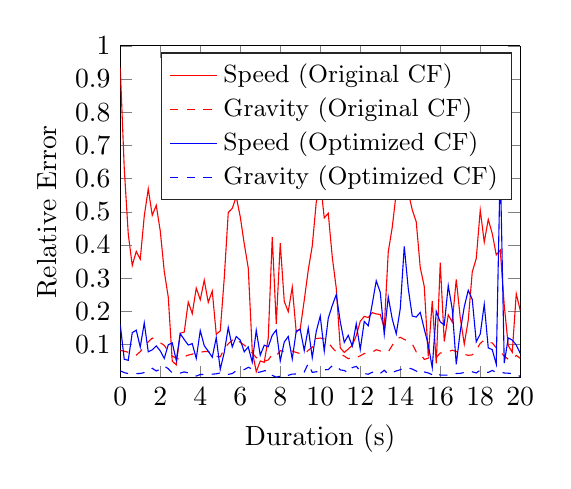
\begin{tikzpicture}

\begin{axis}[%
width= 2in,
height=1.66in,
at={(1.010315in,0.641161in)},
scale only axis,
separate axis lines,
every outer x axis line/.append style={black},
every x tick label/.append style={font=\color{black}},
xmin=0,
xmax=20,
xlabel={Duration (s)},
ytick={0.1,0.2,...,1,1.1},
xtick={0,2,...,18,20},
every outer y axis line/.append style={black},
every y tick label/.append style={font=\color{black}},
ymin=0,
ymax=1,
ylabel={Relative Error},
legend style={legend cell align=left,align=left,draw=white!15!black,font=\small}
]

\addplot [color=red,solid]
  table[row sep=crcr]{%
0	0.934178425411703\\
0.2	0.630711086314392\\
0.4	0.433207149033613\\
0.6	0.338195027006401\\
0.8	0.380698182203954\\
1	0.357269608089743\\
1.2	0.48695694180743\\
1.4	0.569026455193306\\
1.6	0.489272406814653\\
1.8	0.5195927825645\\
2	0.442462678956739\\
2.2	0.32036321238541\\
2.4	0.243054093162164\\
2.6	0.0501321584239941\\
2.8	0.0389282199766352\\
3	0.134327351732061\\
3.2	0.137767659179017\\
3.4	0.22811406027044\\
3.6	0.193318908117746\\
3.8	0.270154309193216\\
4	0.235097881467772\\
4.2	0.29403682698472\\
4.4	0.227125912854242\\
4.6	0.261260714091857\\
4.8	0.131136422272064\\
5	0.141269666761689\\
5.2	0.300402703886449\\
5.4	0.497749514543462\\
5.6	0.510103866058074\\
5.8	0.545311466214906\\
6	0.485040378166185\\
6.2	0.403372936697932\\
6.4	0.330901561265588\\
6.6	0.0802111351412425\\
6.8	0.0183589748131671\\
7	0.0505801484928645\\
7.2	0.0466992184761178\\
7.4	0.119835722977596\\
7.6	0.42368587058199\\
7.8	0.162580517896967\\
8	0.40527371346772\\
8.2	0.230247168870699\\
8.4	0.199232696702737\\
8.6	0.273108853399689\\
8.8	0.136840364675163\\
9	0.148232456751419\\
9.2	0.233772041327655\\
9.4	0.324366499288607\\
9.6	0.397003628093189\\
9.8	0.528500242972586\\
10	0.593033556217057\\
10.2	0.481390855611857\\
10.4	0.495688688526854\\
10.6	0.364177215944165\\
10.8	0.269906025482089\\
11	0.089955710217472\\
11.2	0.0764230292564081\\
11.4	0.0864444158710254\\
11.6	0.0977203303198929\\
11.8	0.126967314618481\\
12	0.170162074749627\\
12.2	0.184850798617868\\
12.4	0.181665518045507\\
12.6	0.196148642920703\\
12.8	0.192382231103711\\
13	0.190681813470425\\
13.2	0.15005104357931\\
13.4	0.379155460391126\\
13.6	0.453325962924387\\
13.8	0.558025857479416\\
14	0.590909743554408\\
14.2	0.655814984671255\\
14.4	0.559922096611395\\
14.6	0.505859066347001\\
14.8	0.469665176929225\\
15	0.331923771381844\\
15.2	0.275237886825183\\
15.4	0.0648993527114071\\
15.6	0.231668997156276\\
15.8	0.0431828511228876\\
16	0.346815580289996\\
16.2	0.109466200504509\\
16.4	0.189516727077678\\
16.6	0.167990602193994\\
16.8	0.296292110186219\\
17	0.181237086631773\\
17.2	0.101173896288763\\
17.4	0.173092376561692\\
17.6	0.31877142005269\\
17.8	0.359156201495661\\
18	0.505334402114304\\
18.2	0.408680827325729\\
18.4	0.477082835390875\\
18.6	0.43429316898945\\
18.8	0.37010249134627\\
19	0.384592309719538\\
19.2	0.21793842687793\\
19.4	0.0967790197067872\\
19.6	0.0769282381005661\\
19.8	0.253045687028195\\
20	0.203032358736927\\
};
\addlegendentry{Speed (Original CF)};

\addplot [color=red,dashed]
  table[row sep=crcr]{%
0	0.0822919686729097\\
0.2	0.0802019234810112\\
0.4	0.0767994537012122\\
0.6	0.0710381075680924\\
0.8	0.0681695393729234\\
1	0.0788803330458938\\
1.2	0.095128489126129\\
1.4	0.108416707342104\\
1.6	0.119631175769165\\
1.8	0.111652297183521\\
2	0.105565009013153\\
2.2	0.097624817057137\\
2.4	0.0798737029173406\\
2.6	0.0652493681188569\\
2.8	0.0596648330242322\\
3	0.0543194856618239\\
3.2	0.063139710181382\\
3.4	0.0684801560051139\\
3.6	0.07106233870063\\
3.8	0.0761739845777189\\
4	0.0762559785064391\\
4.2	0.0793445652312052\\
4.4	0.07861747093658\\
4.6	0.0743846955230543\\
4.8	0.0646530325268517\\
5	0.0632091463713744\\
5.2	0.086451563272956\\
5.4	0.102385566973736\\
5.6	0.113317963910957\\
5.8	0.119909242130471\\
6	0.106835407382745\\
6.2	0.0982427171271348\\
6.4	0.0887874710082105\\
6.6	0.074323821164016\\
6.8	0.0608806554070442\\
7	0.0546751973473795\\
7.2	0.0498121845590002\\
7.4	0.0537900973915386\\
7.6	0.0699729984537361\\
7.8	0.0654920118382917\\
8	0.0819098435472358\\
8.2	0.0787699019807739\\
8.4	0.083554865563059\\
8.6	0.0804416185618373\\
8.8	0.0763299626810223\\
9	0.0727480637867167\\
9.2	0.0707780814126987\\
9.4	0.0826864571081625\\
9.6	0.0918687230897811\\
9.8	0.117912879917265\\
10	0.119734736721591\\
10.2	0.116887020668105\\
10.4	0.106584649391566\\
10.6	0.0907837501132486\\
10.8	0.0776501957430045\\
11	0.0711799526370746\\
11.2	0.0653688369108648\\
11.4	0.0574853677364737\\
11.6	0.060665434369229\\
11.8	0.0608818875461767\\
12	0.0661899745760615\\
12.2	0.0729901772418144\\
12.4	0.0749980739522499\\
12.6	0.0771633891948391\\
12.8	0.0844806366020025\\
13	0.0807721239106627\\
13.2	0.0777176946527234\\
13.4	0.078002358327407\\
13.6	0.0975323832740162\\
13.8	0.116310810906317\\
14	0.121989043251718\\
14.2	0.115537596604213\\
14.4	0.110496657822582\\
14.6	0.101792048066162\\
14.8	0.0777696515176027\\
15	0.0740299347198575\\
15.2	0.0551619420909771\\
15.4	0.0590309064402883\\
15.6	0.0691013918386351\\
15.8	0.060847643061093\\
16	0.0746667324774949\\
16.2	0.0761360279732322\\
16.4	0.0781215232191581\\
16.6	0.0832297637020978\\
16.8	0.0786810051222752\\
17	0.0768991646453432\\
17.2	0.0707839052927942\\
17.4	0.0675375225422769\\
17.6	0.0689210411607286\\
17.8	0.0839741594955832\\
18	0.103532463698234\\
18.2	0.113877815050963\\
18.4	0.105155790473866\\
18.6	0.105274035807157\\
18.8	0.0903022762734443\\
19	0.0797115476001153\\
19.2	0.0647106685911285\\
19.4	0.0560078130292158\\
19.6	0.0550408767784075\\
19.8	0.0673701675058704\\
20	0.0585255130554378\\
};
\addlegendentry{Gravity (Original CF)};

\addplot [color=blue,solid]
  table[row sep=crcr]{%
0	0.159789211041408\\
0.2	0.055818980601535\\
0.4	0.0526352128821143\\
0.6	0.135802330438254\\
0.8	0.143535467060861\\
1	0.0924335125097111\\
1.2	0.165235611081226\\
1.4	0.0782795384513208\\
1.6	0.0840504500016598\\
1.8	0.0961690213028328\\
2	0.0811744526638112\\
2.2	0.0582195002126566\\
2.4	0.0991583642963534\\
2.6	0.105186386220957\\
2.8	0.0525522029567892\\
3	0.132642854540067\\
3.2	0.115156851742683\\
3.4	0.0986050097729008\\
3.6	0.102842420391244\\
3.8	0.0584264467342688\\
4	0.14219250140189\\
4.2	0.096606371109511\\
4.4	0.0801137831255749\\
4.6	0.0619433399786171\\
4.8	0.120671296887563\\
5	0.0253336490061051\\
5.2	0.0765854290744431\\
5.4	0.151542827573333\\
5.6	0.0929257754121167\\
5.8	0.124281864934116\\
6	0.113329576674137\\
6.2	0.0783663134287818\\
6.4	0.0929446249150401\\
6.6	0.0472563880129299\\
6.8	0.143016309925407\\
7	0.0678892895754403\\
7.2	0.0982383180146145\\
7.4	0.0933507807258168\\
7.6	0.128009779946219\\
7.8	0.143885599773393\\
8	0.0507775717220851\\
8.2	0.107716362501048\\
8.4	0.124442505882418\\
8.6	0.0564263879184188\\
8.8	0.140848715663291\\
9	0.145558477256298\\
9.2	0.0819966813393724\\
9.4	0.149977464234889\\
9.6	0.0606168418321929\\
9.8	0.139452084109503\\
10	0.185929027011773\\
10.2	0.0805074422480105\\
10.4	0.17918262551508\\
10.6	0.217580299028164\\
10.8	0.250442612490507\\
11	0.169365448756039\\
11.2	0.106661406527292\\
11.4	0.127853443868295\\
11.6	0.0955396618949333\\
11.8	0.162897404879062\\
12	0.0855595459857846\\
12.2	0.169672845515126\\
12.4	0.15669225162091\\
12.6	0.222441046723326\\
12.8	0.292222929720095\\
13	0.257402501738607\\
13.2	0.131180164180187\\
13.4	0.243743166109111\\
13.6	0.176879810534277\\
13.8	0.132524225273731\\
14	0.207869235646211\\
14.2	0.395964879962667\\
14.4	0.269007358951566\\
14.6	0.185934873588351\\
14.8	0.18308571773916\\
15	0.196960199690523\\
15.2	0.146819923617054\\
15.4	0.0992783810197273\\
15.6	0.0304878022407633\\
15.8	0.200001692869642\\
16	0.168145207419985\\
16.2	0.159066378919115\\
16.4	0.277866062460796\\
16.6	0.206515484223874\\
16.8	0.0407954153277216\\
17	0.140047439957052\\
17.2	0.213676941339341\\
17.4	0.263524793596698\\
17.6	0.236252458544446\\
17.8	0.107988934149429\\
18	0.131868606673165\\
18.2	0.221410249239274\\
18.4	0.0902149392751371\\
18.6	0.0845994749385033\\
18.8	0.041314092208996\\
19	0.644110499431759\\
19.2	0.0440755152670826\\
19.4	0.120100843123323\\
19.6	0.113664265680662\\
19.8	0.098717923319369\\
20	0.0737252149881171\\
};
\addlegendentry{Speed (Optimized CF)};

\addplot [color=blue,dashed]
  table[row sep=crcr]{%
0	0.0210356936642969\\
0.2	0.0156500878588521\\
0.4	0.0124379735226696\\
0.6	0.0131401752363818\\
0.8	0.0126249775551881\\
1	0.0129743224587194\\
1.2	0.0156144562852086\\
1.4	0.0180139626733828\\
1.6	0.0286147522195074\\
1.8	0.0203997777172854\\
2	0.0264346774724002\\
2.2	0.0352082224156913\\
2.4	0.0272809063095656\\
2.6	0.0145158878157373\\
2.8	0.0141873423326073\\
3	0.0141504777353216\\
3.2	0.017661915502658\\
3.4	0.0146514104842404\\
3.6	0.00848739045651757\\
3.8	0.00524427338839714\\
4	0.00980663288325618\\
4.2	0.00980079862328375\\
4.4	0.00962598456842894\\
4.6	0.010855146200219\\
4.8	0.0120023801298546\\
5	0.0145220565720842\\
5.2	0.00945801373580289\\
5.4	0.0102022775550055\\
5.6	0.0128367072955619\\
5.8	0.0212448038024438\\
6	0.0227230319322569\\
6.2	0.0246580620512529\\
6.4	0.0314790076131019\\
6.6	0.0265633409117838\\
6.8	0.0157208426573386\\
7	0.0173398447483718\\
7.2	0.0210676568884499\\
7.4	0.0214458306562988\\
7.6	0.00728337040030744\\
7.8	0.0018863162524225\\
8	0.00494367752926812\\
8.2	0.00387545132462198\\
8.4	0.00740696517412505\\
8.6	0.0111265981728175\\
8.8	0.011402513494496\\
9	0.0113941204005887\\
9.2	0.0173362798165867\\
9.4	0.0433288768973993\\
9.6	0.0161494313508156\\
9.8	0.0181420868819509\\
10	0.0190802680872845\\
10.2	0.0242196169841968\\
10.4	0.0244902255417225\\
10.6	0.0362859020132688\\
10.8	0.0370025302863598\\
11	0.023718340376067\\
11.2	0.0218690004694039\\
11.4	0.0149649988525665\\
11.6	0.0307483645754441\\
11.8	0.034257636101975\\
12	0.021447316427866\\
12.2	0.0129453652000109\\
12.4	0.0106830480040495\\
12.6	0.0168083567575575\\
12.8	0.00920827709028584\\
13	0.0131934797210005\\
13.2	0.0226115864114399\\
13.4	0.0106012478323422\\
13.6	0.0162992685514342\\
13.8	0.0205112560454778\\
14	0.0242790233819461\\
14.2	0.0302925414436663\\
14.4	0.0298239317730862\\
14.6	0.0262404146305944\\
14.8	0.020442059098999\\
15	0.01175730666464\\
15.2	0.0175760126723965\\
15.4	0.0144554361177308\\
15.6	0.00924989677601856\\
15.8	0.0154883836316607\\
16	0.00815148135728055\\
16.2	0.00819297898819766\\
16.4	0.00763318558096878\\
16.6	0.0116791020264973\\
16.8	0.0129049990107104\\
17	0.0132644896643077\\
17.2	0.0161546696486076\\
17.4	0.0177022115217355\\
17.6	0.0180775098929127\\
17.8	0.0144444401354602\\
18	0.0231496515123869\\
18.2	0.0191588248503959\\
18.4	0.0159567398510836\\
18.6	0.022213026609365\\
18.8	0.0162879860573466\\
19	0.0181156341764785\\
19.2	0.0144059097859136\\
19.4	0.0137554211208593\\
19.6	0.0127632633250231\\
19.8	0.0105231343121108\\
20	0.00392609585910132\\
};
\addlegendentry{Gravity (Optimized CF)};
\end{axis}
\end{tikzpicture}%
}
    \caption{Artificial bias of magnitude $0.05 rad/s$.\label{fig:validBias1}}
  \end{subfigure}
  \begin{subfigure}[b]{0.489\columnwidth}
    \resizebox{\columnwidth}{!}{% This file was created by matlab2tikz.
% Minimal pgfplots version: 1.3
%
%The latest updates can be retrieved from
%  http://www.mathworks.com/matlabcentral/fileexchange/22022-matlab2tikz
%where you can also make suggestions and rate matlab2tikz.
%
\definecolor{mycolor1}{rgb}{1.00000,0.00000,1.00000}%
%
\begin{tikzpicture}

\begin{axis}[%
width=6.023032in,
height=4.750423in,
at={(1.010315in,0.641161in)},
scale only axis,
separate axis lines,
every outer x axis line/.append style={black},
every x tick label/.append style={font=\color{black}},
xmin=0,
xmax=20,
xlabel={Duration (s)},
every outer y axis line/.append style={black},
every y tick label/.append style={font=\color{black}},
ymin=0,
ymax=1,
ylabel={Error (\%)},
legend style={legend cell align=left,align=left,draw=black}
]
\addplot [color=blue,solid]
  table[row sep=crcr]{%
0	0\\
0.2	0\\
0.4	0\\
0.6	0\\
0.8	0\\
1	0\\
1.2	0\\
1.4	0\\
1.6	0\\
1.8	0\\
2	0\\
2.2	0\\
2.4	0\\
2.6	0\\
2.8	0\\
3	0\\
3.2	0\\
3.4	0\\
3.6	0\\
3.8	0\\
4	0\\
4.2	0\\
4.4	0\\
4.6	0\\
4.8	0\\
5	0\\
5.2	0\\
5.4	0\\
5.6	0\\
5.8	0\\
6	0\\
6.2	0\\
6.4	0\\
6.6	0\\
6.8	0\\
7	0\\
7.2	0\\
7.4	0\\
7.6	0\\
7.8	0\\
8	0\\
8.2	0\\
8.4	0\\
8.6	0\\
8.8	0\\
9	0\\
9.2	0\\
9.4	0\\
9.6	0\\
9.8	0\\
10	0\\
10.2	0\\
10.4	0\\
10.6	0\\
10.8	0\\
11	0\\
11.2	0\\
11.4	0\\
11.6	0\\
11.8	0\\
12	0\\
12.2	0\\
12.4	0\\
12.6	0\\
12.8	0\\
13	0\\
13.2	0\\
13.4	0\\
13.6	0\\
13.8	0\\
14	0\\
14.2	0\\
14.4	0\\
14.6	0\\
14.8	0\\
15	0\\
15.2	0\\
15.4	0\\
15.6	0\\
15.8	0\\
16	0\\
16.2	0\\
16.4	0\\
16.6	0\\
16.8	0\\
17	0\\
17.2	0\\
17.4	0\\
17.6	0\\
17.8	0\\
18	0\\
18.2	0\\
18.4	0\\
18.6	0\\
18.8	0\\
19	0\\
19.2	0\\
19.4	0\\
19.6	0\\
19.8	0\\
20	0\\
};
\addlegendentry{lambda};

\addplot [color=red,solid]
  table[row sep=crcr]{%
0	1.64919690621323\\
0.2	1.17447277686694\\
0.4	0.857214476919527\\
0.6	0.72373456395983\\
0.8	0.722961002477919\\
1	0.778198112958438\\
1.2	0.864181507358116\\
1.4	0.932956598977546\\
1.6	0.874547508675396\\
1.8	0.828425978163367\\
2	0.736188311203124\\
2.2	0.588450103224406\\
2.4	0.457965869753184\\
2.6	0.136938451920545\\
2.8	0.0616249828557932\\
3	0.198749964919302\\
3.2	0.282285010295693\\
3.4	0.440283357186753\\
3.6	0.408133758780261\\
3.8	0.507038065084139\\
4	0.453167663905494\\
4.2	0.510562609997532\\
4.4	0.433077086700963\\
4.6	0.435856533985514\\
4.8	0.256949137683949\\
5	0.32651217819208\\
5.2	0.553893222501443\\
5.4	0.853482293054466\\
5.6	0.849788583501695\\
5.8	0.85213865269188\\
6	0.793705707067439\\
6.2	0.691937023244995\\
6.4	0.600848915242407\\
6.6	0.220951326152415\\
6.8	0.143480436596722\\
7	0.0603083163191883\\
7.2	0.0746436240511588\\
7.4	0.280862719079441\\
7.6	0.73978860220415\\
7.8	0.354579140584992\\
8	0.691282810240332\\
8.2	0.447016020856702\\
8.4	0.419492047451668\\
8.6	0.498016237134613\\
8.8	0.311889125041271\\
9	0.268272183586567\\
9.2	0.41713655835746\\
9.4	0.588080133884643\\
9.6	0.732582034424561\\
9.8	0.863883214819874\\
10	0.875825972330869\\
10.2	0.804648341670244\\
10.4	0.749692330287877\\
10.6	0.559451976347465\\
10.8	0.376529338535504\\
11	0.125706737435439\\
11.2	0.0824355916322666\\
11.4	0.128538705384917\\
11.6	0.222516715516052\\
11.8	0.225881933135957\\
12	0.395278734237151\\
12.2	0.382477009252591\\
12.4	0.386373499392455\\
12.6	0.378573924384842\\
12.8	0.338450630628311\\
13	0.337811620226246\\
13.2	0.272169789929263\\
13.4	0.534239975027235\\
13.6	0.685982321966463\\
13.8	0.845028476864752\\
14	0.862433283289276\\
14.2	0.865920173316997\\
14.4	0.808205655603995\\
14.6	0.766724900926839\\
14.8	0.69173539601179\\
15	0.432271948933186\\
15.2	0.370991188327238\\
15.4	0.0702139992845107\\
15.6	0.440495840150363\\
15.8	0.164106394665433\\
16	0.55593294976504\\
16.2	0.302642170159351\\
16.4	0.303154761410595\\
16.6	0.374486789470867\\
16.8	0.514274305330887\\
17	0.39104158425063\\
17.2	0.250916458779965\\
17.4	0.238783344706397\\
17.6	0.483420726277381\\
17.8	0.645659213652222\\
18	0.78192565482982\\
18.2	0.816909914371338\\
18.4	0.798072574976972\\
18.6	0.759615463804278\\
18.8	0.67194041235707\\
19	0.47858781024885\\
19.2	0.41939508931665\\
19.4	0.11862362945303\\
19.6	0.0550843427311009\\
19.8	0.480074690638293\\
20	0.378384177262263\\
};
\addlegendentry{speed};

\addplot [color=mycolor1,solid]
  table[row sep=crcr]{%
0	0.141746603249912\\
0.2	0.137750831538313\\
0.4	0.130767017855888\\
0.6	0.12467282778485\\
0.8	0.125877506547112\\
1	0.143514740475512\\
1.2	0.16533397358608\\
1.4	0.182792683549569\\
1.6	0.194330747685901\\
1.8	0.184502983591167\\
2	0.173421421699709\\
2.2	0.157462469742407\\
2.4	0.130961707561024\\
2.6	0.108114184900927\\
2.8	0.100080674990977\\
3	0.0908327697194296\\
3.2	0.108347702489179\\
3.4	0.122801043641573\\
3.6	0.128196011562677\\
3.8	0.137454869843851\\
4	0.137526685816278\\
4.2	0.138581322937122\\
4.4	0.134759148115883\\
4.6	0.129616053128364\\
4.8	0.117361651791967\\
5	0.117718294346329\\
5.2	0.150677991207567\\
5.4	0.178321307122113\\
5.6	0.190607240029868\\
5.8	0.196980758121016\\
6	0.181027594730807\\
6.2	0.165073614495852\\
6.4	0.147635851539372\\
6.6	0.124841858359997\\
6.8	0.102163469858529\\
7	0.0920280987517897\\
7.2	0.0891872194877835\\
7.4	0.100665123559182\\
7.6	0.134201447673728\\
7.8	0.122428955949035\\
8	0.14735234691071\\
8.2	0.13859940329675\\
8.4	0.146166304484341\\
8.6	0.141315926809646\\
8.8	0.13134449322759\\
9	0.128240922653559\\
9.2	0.125518782009188\\
9.4	0.146453436767666\\
9.6	0.166628894391061\\
9.8	0.195841448473604\\
10	0.197208053880588\\
10.2	0.190716366719807\\
10.4	0.173973449255969\\
10.6	0.148387288443183\\
10.8	0.126945928694347\\
11	0.116892551652998\\
11.2	0.0997329931803297\\
11.4	0.0957084698179621\\
11.6	0.107023468705138\\
11.8	0.112947127142971\\
12	0.124403955115649\\
12.2	0.132581455470047\\
12.4	0.135054553932841\\
12.6	0.136914701355096\\
12.8	0.139403592014042\\
13	0.134283688336299\\
13.2	0.129954526042869\\
13.4	0.133694307861919\\
13.6	0.162910810406651\\
13.8	0.190661406584853\\
14	0.198424160455334\\
14.2	0.191185318874325\\
14.4	0.183856279753217\\
14.6	0.169706918366894\\
14.8	0.137317865506257\\
15	0.123200083303233\\
15.2	0.0955788908416441\\
15.4	0.0981569337080104\\
15.6	0.123317504310104\\
15.8	0.106270603646884\\
16	0.12744868201445\\
16.2	0.133116521388984\\
16.4	0.137462628052843\\
16.6	0.147754506457766\\
16.8	0.138168262789613\\
17	0.13417864017689\\
17.2	0.12509790803965\\
17.4	0.119577734122555\\
17.6	0.125147259042934\\
17.8	0.150715495574359\\
18	0.176545164829519\\
18.2	0.193994340926104\\
18.4	0.182314197734155\\
18.6	0.178990020587585\\
18.8	0.157518933077857\\
19	0.137761855103257\\
19.2	0.112511520633163\\
19.4	0.0962468454328662\\
19.6	0.0942326861817091\\
19.8	0.122811328765315\\
20	0.107009786553117\\
};
\addlegendentry{gravity};

\addplot [color=blue,dashed,forget plot]
  table[row sep=crcr]{%
0	0\\
0.2	0\\
0.4	0\\
0.6	0\\
0.8	0\\
1	0\\
1.2	0\\
1.4	0\\
1.6	0\\
1.8	0\\
2	0\\
2.2	0\\
2.4	0\\
2.6	0\\
2.8	0\\
3	0\\
3.2	0\\
3.4	0\\
3.6	0\\
3.8	0\\
4	0\\
4.2	0\\
4.4	0\\
4.6	0\\
4.8	0\\
5	0\\
5.2	0\\
5.4	0\\
5.6	0\\
5.8	0\\
6	0\\
6.2	0\\
6.4	0\\
6.6	0\\
6.8	0\\
7	0\\
7.2	0\\
7.4	0\\
7.6	0\\
7.8	0\\
8	0\\
8.2	0\\
8.4	0\\
8.6	0\\
8.8	0\\
9	0\\
9.2	0\\
9.4	0\\
9.6	0\\
9.8	0\\
10	0\\
10.2	0\\
10.4	0\\
10.6	0\\
10.8	0\\
11	0\\
11.2	0\\
11.4	0\\
11.6	0\\
11.8	0\\
12	0\\
12.2	0\\
12.4	0\\
12.6	0\\
12.8	0\\
13	0\\
13.2	0\\
13.4	0\\
13.6	0\\
13.8	0\\
14	0\\
14.2	0\\
14.4	0\\
14.6	0\\
14.8	0\\
15	0\\
15.2	0\\
15.4	0\\
15.6	0\\
15.8	0\\
16	0\\
16.2	0\\
16.4	0\\
16.6	0\\
16.8	0\\
17	0\\
17.2	0\\
17.4	0\\
17.6	0\\
17.8	0\\
18	0\\
18.2	0\\
18.4	0\\
18.6	0\\
18.8	0\\
19	0\\
19.2	0\\
19.4	0\\
19.6	0\\
19.8	0\\
20	0\\
};
\addplot [color=red,dashed,forget plot]
  table[row sep=crcr]{%
0	0.205222987720891\\
0.2	0.0726747181388864\\
0.4	0.0542042347671224\\
0.6	0.142825360065919\\
0.8	0.138430888961027\\
1	0.0930054865401621\\
1.2	0.165756017083899\\
1.4	0.066158106121503\\
1.6	0.120773766156876\\
1.8	0.0817088837311307\\
2	0.0696813480518532\\
2.2	0.0549409008501835\\
2.4	0.0803185674913163\\
2.6	0.161798538898003\\
2.8	0.0954684324876172\\
3	0.225945436131043\\
3.2	0.183492160972187\\
3.4	0.0977984685165634\\
3.6	0.0900651164048965\\
3.8	0.0643782317450595\\
4	0.14937166261992\\
4.2	0.103692805044996\\
4.4	0.101899027832279\\
4.6	0.059660216758595\\
4.8	0.111539732309505\\
5	0.0553387196215443\\
5.2	0.0859292795044416\\
5.4	0.178024650275305\\
5.6	0.11463710422396\\
5.8	0.104830149576218\\
6	0.106586863347681\\
6.2	0.0705460275734378\\
6.4	0.0878556208175251\\
6.6	0.0527690923654345\\
6.8	0.196228754571483\\
7	0.114540863177281\\
7.2	0.155631535436674\\
7.4	0.156294421050576\\
7.6	0.164870048421171\\
7.8	0.125073149968079\\
8	0.0483671565800194\\
8.2	0.112739014871651\\
8.4	0.13795214680356\\
8.6	0.0625029183777485\\
8.8	0.150985444240664\\
9	0.139956515284906\\
9.2	0.0723710178639838\\
9.4	0.116033073095249\\
9.6	0.100205584993715\\
9.8	0.151494988320149\\
10	0.159139125491527\\
10.2	0.0835224420919841\\
10.4	0.164661633145721\\
10.6	0.207671339982477\\
10.8	0.234607847296393\\
11	0.132964998961677\\
11.2	0.0674764060253643\\
11.4	0.100417037755404\\
11.6	0.105609494370976\\
11.8	0.14007783575226\\
12	0.0788964335917637\\
12.2	0.164876319608772\\
12.4	0.164053281683847\\
12.6	0.238480566140862\\
12.8	0.311274795466956\\
13	0.267748557155861\\
13.2	0.119861244062927\\
13.4	0.224458289617256\\
13.6	0.149205247290263\\
13.8	0.0944377904306769\\
14	0.170124076206034\\
14.2	0.375181686946106\\
14.4	0.258444172565526\\
14.6	0.169985454148999\\
14.8	0.166662405701909\\
15	0.181011082746411\\
15.2	0.127505508413763\\
15.4	0.162740877698488\\
15.6	0.101204644525866\\
15.8	0.1907029679991\\
16	0.219051335625323\\
16.2	0.144661615785364\\
16.4	0.274865236829768\\
16.6	0.21605933152686\\
16.8	0.0386789370592563\\
17	0.159522070741464\\
17.2	0.223093348896405\\
17.4	0.252312115407037\\
17.6	0.209680197265715\\
17.8	0.114755789545134\\
18	0.0870331769830534\\
18.2	0.255864229439525\\
18.4	0.0762541316470259\\
18.6	0.0892521141216874\\
18.8	0.0401461417153033\\
19	0.677119316260807\\
19.2	0.054450265674583\\
19.4	0.189328189059458\\
19.6	0.095507061068136\\
19.8	0.16066855386482\\
20	0.105287766550178\\
};
\addplot [color=mycolor1,dashed,forget plot]
  table[row sep=crcr]{%
0	0.0265593391640491\\
0.2	0.0190902322281718\\
0.4	0.0150027771426299\\
0.6	0.0141401038660383\\
0.8	0.0134270898645597\\
1	0.0135703727162123\\
1.2	0.0150162522178532\\
1.4	0.0182424786108652\\
1.6	0.0263627930806009\\
1.8	0.0173085902032298\\
2	0.0232190253453376\\
2.2	0.0322515729025285\\
2.4	0.0226124231168771\\
2.6	0.0123351131473082\\
2.8	0.0241499136310865\\
3	0.0265771809043431\\
3.2	0.0263028652250568\\
3.4	0.0191895372462108\\
3.6	0.0107215490761968\\
3.8	0.00542308960323552\\
4	0.0129466142932514\\
4.2	0.0131025535210239\\
4.4	0.0146913032504019\\
4.6	0.0140068121442529\\
4.8	0.0107552516525201\\
5	0.00949316791590398\\
5.2	0.00723204281234885\\
5.4	0.0133721538883133\\
5.6	0.012010325846133\\
5.8	0.0185332665075269\\
6	0.0209900556104048\\
6.2	0.0211375850899186\\
6.4	0.0273712828733141\\
6.6	0.0240441664453908\\
6.8	0.0201727287823399\\
7	0.027508825566898\\
7.2	0.0338754688695914\\
7.4	0.0322953927273036\\
7.6	0.0100441852851962\\
7.8	0.00467740907916177\\
8	0.00589903392617338\\
8.2	0.00545539670771769\\
8.4	0.00981929415167433\\
8.6	0.0130718488470684\\
8.8	0.0126706757113732\\
9	0.0101607462754941\\
9.2	0.0128255400536001\\
9.4	0.0395430611396309\\
9.6	0.0115162948912323\\
9.8	0.0157185592682899\\
10	0.0161395636924551\\
10.2	0.0223380643746207\\
10.4	0.0214282852603132\\
10.6	0.0339805599911967\\
10.8	0.0335605378203179\\
11	0.0211193401673884\\
11.2	0.0267114466508416\\
11.4	0.0253242850528746\\
11.6	0.0407938044300684\\
11.8	0.040451466791767\\
12	0.0234400762112916\\
12.2	0.0132559759777615\\
12.4	0.0126278393607724\\
12.6	0.0212211030207641\\
12.8	0.0142008833745218\\
13	0.0173775956539004\\
13.2	0.020789482154874\\
13.4	0.00799621104263157\\
13.6	0.0131026719020416\\
13.8	0.0207508716806424\\
14	0.0219792767160374\\
14.2	0.027937408291671\\
14.4	0.0272528775726367\\
14.6	0.0227459923058363\\
14.8	0.0218109677458626\\
15	0.0102827347116005\\
15.2	0.027754787966455\\
15.4	0.024828152833262\\
15.6	0.0132943332334685\\
15.8	0.0111260921556311\\
16	0.0106171197850443\\
16.2	0.0103045472025132\\
16.4	0.00710238219602398\\
16.6	0.0113425077732525\\
16.8	0.01457663496832\\
17	0.0168351386607923\\
17.2	0.019339139320766\\
17.4	0.0153651271504735\\
17.6	0.0132172711212311\\
17.8	0.0091257168100364\\
18	0.0256203434996566\\
18.2	0.0165257045516403\\
18.4	0.0109151619070869\\
18.6	0.0181257710994386\\
18.8	0.012228172242146\\
19	0.0138612536863584\\
19.2	0.0181175766564797\\
19.4	0.022643110915269\\
19.6	0.0243671059835327\\
19.8	0.0199521749261112\\
20	0.00991437110007944\\
};
\end{axis}
\end{tikzpicture}%}
    \caption{Artificial bias of magnitude $0.1 rad/s$.\label{fig:validBias2}}
  \end{subfigure}
  \caption{Estimation error of the optimized closed-form solution against the original closed-form solution \cite{Martinelli2014} and SVO \cite{FaesslerICRA15}.
    The duration of integration is set to 2.8 seconds, and 10 point features are observed throughout the whole operation.
    In Fig. \ref{fig:validBias1} and Fig. \ref{fig:validBias1}, we corrupted the gyroscope measurements with an artificial bias.}

\end{figure}

%In a real applications, a proper online computation of the gyroscope bias can be reused.
%% Since the gyroscope bias varies slowly over time, we can reuse its knowledge.
%% In other words, we can use the optimized closed-form solution to compute the bias at the beginning of the sequence.
%% Thereafter, we can quickly provide reliable state estimations with the standard closed-form solution by compensating with the computed bias.

%% For long term navigation (longer than a minute), it would be advised to recompute the gyroscope bias every so often.
%% This re-computation can use the knowledge of previously computed bias. % as stated in Section \ref{sec:reg}.

%% The reason why we do not run the optimization for every state estimation is to speed up the computation.
%% Despite the optimization is relatively fast since our cost function is defined only with respect to the gyroscope bias, it still has to run the closed-form solution several times for its gradient descent to converge.
%% We found by experimentation that it usually requires around 6 iterations to converge.


\section{CONCLUSION}\label{SectionConclusion}

%For an MAV, limiting the number of on-board sensor is important to save power consumption and processing power.
%A popular choice of sensors is a camera coupled with an IMU for their complementary.
%However, the methods for fusing visual and inertial measurements so far introduced are filter based, hence require an initialization.
%Providing a reliable state initialization is critical for these algorithms to work correctly.

In this paper, we studied the recent closed-form solution proposed by \cite{Martinelli2014} which performs visual-inertial sensor fusion without requiring an initialization.
We implemented this method in order to test it with plausible MAV motions and synthetic noisy sensor data.
This allowed us to identify its performance limitations and bring modifications to overcome them.
We investigated the impact of biased inertial measurements.
Although the case of biased accelerometer was originally studied in \cite{Martinelli2014}, we showed that the accelerometer bias does not significantly worsen the performance.
One major performance limitation of this method was due to the impact of biased gyroscope measurements.
In other words, the performance becomes very poor in presence of a bias on the gyroscope and, in practice, the overall method could only be successfully used with a very precise (and expensive) gyroscope.
We then introduced a simple method that automatically estimates this bias.
We validated this method by comparing its performance against state-of-the-art pose estimation approach for MAV.
For future work, we see this optimized closed-form solution being used on an MAV to provide accurate state initialization.
This would allow aggressive take-off maneuvers, such as hand throwing the MAV in the air, as already demonstrated in \cite{Faessler2015} with a range sensor.
With our technique, we could get rid of the range sensor.

\printbibliography

\end{document}
